\documentclass[11pt]{article}
\newcommand{\doctype}{Technical report}
\newcommand{\docversion}{v0.01.002}
\newcommand{\docdate}{2 November 2026}
\newcommand{\versiondoi}{10.5281/zenodo.23899079}
\newcommand{\conceptdoi}{10.5281/zenodo.23851659}
\newcommand{\docrepo}{github.com/fsantibanezleal/CAOS\_SoftQP}
\newcommand{\docscope}{soft-constraint quadratic programming}
\newcommand{\shorttitle}{Soft-constraint QP methods}
% Presentation derived from the canonical CAOS Research foundational article.
\usepackage[T1]{fontenc}
\usepackage[utf8]{inputenc}
\usepackage{lmodern,microtype}
\usepackage[margin=1.1in,headheight=15pt]{geometry}
\usepackage{amsmath,amssymb,amsthm}
\usepackage{booktabs,array,tabularx,longtable,graphicx}
\usepackage{algorithm,algpseudocode}
\usepackage{xcolor,xurl}
\definecolor{linknavy}{RGB}{25,55,125}
\usepackage[colorlinks=true,linkcolor=linknavy,citecolor=linknavy,urlcolor=linknavy]{hyperref}
\usepackage{orcidlink}
\usepackage{fancyhdr}
\newtheorem{theorem}{Theorem}[section]
\newtheorem{proposition}[theorem]{Proposition}
\newtheorem{lemma}[theorem]{Lemma}
\theoremstyle{definition}
\newtheorem{definition}[theorem]{Definition}
\theoremstyle{remark}
\newtheorem{remark}[theorem]{Remark}
\DeclareMathOperator{\prox}{prox}
\DeclareMathOperator{\diag}{diag}
\DeclareMathOperator{\median}{median}
\DeclareMathOperator{\argmin}{argmin}
\newcommand{\R}{\mathbb{R}}
\newcommand{\pos}[1]{\left(#1\right)_{+}}
\newcommand{\norm}[1]{\left\lVert#1\right\rVert_{\infty}}
\newcommand{\headerblock}{%
\begin{center}
\fbox{\parbox{0.94\textwidth}{\small\raggedright
\textbf{\doctype} \quad$\cdot$\quad \docversion, \docdate \quad$\cdot$\quad Licence CC BY 4.0\\[2pt]
CAOS Research programme \quad$\cdot$\quad \docscope\\[2pt]
Version DOI \href{https://doi.org/\versiondoi}{\texttt{\versiondoi}}\\[2pt] % voice-ok: required page-one header identity, not body narrative
Concept DOI (always latest) \href{https://doi.org/\conceptdoi}{\texttt{\conceptdoi}}\\[2pt] % voice-ok: required page-one header identity, not body narrative
Not peer reviewed. Source code, data and computational records:
\href{https://\docrepo}{\texttt{\docrepo}}
}}
\end{center}
\vspace{4pt}}
\pagestyle{fancy}
\fancyhf{}
\fancyhead[L]{\small CAOS Research \doctype}
\fancyhead[R]{\small \shorttitle\ \textperiodcentered\ \docversion}
\fancyfoot[C]{\small \thepage}
\renewcommand{\headrulewidth}{0.4pt}
\fancypagestyle{plain}{\fancyhf{}\fancyfoot[C]{\small \thepage}\renewcommand{\headrulewidth}{0pt}}
\setlength{\emergencystretch}{1.5em}

% Numeric export from the reviewed summary; no new inference.
\newcommand{\PrimaryEstimate}{-212.449875}
\newcommand{\PrimaryLower}{-225.336618}
\newcommand{\PrimaryUpper}{-192.873759}
\newcommand{\PrimaryFailed}{9}
\newcommand{\PrimaryPopulation}{144}
\newcommand{\SummaryDigest}{c82bf30bb53c7c10d464fc446bd2b99ee774b581dbe3f4dced86194e1fe54c6d}
\newcommand{\DevelopmentAccepted}{879}
\newcommand{\DevelopmentAccuracyRejected}{0}
\newcommand{\DevelopmentIncompatible}{396}
\newcommand{\DevelopmentOracleFailed}{21}
\newcommand{\DevelopmentTimeout}{0}
\newcommand{\HeldoutAccepted}{2587}
\newcommand{\HeldoutAccuracyRejected}{6}
\newcommand{\HeldoutIncompatible}{1188}
\newcommand{\HeldoutOracleFailed}{105}
\newcommand{\HeldoutTimeout}{2}
\newcommand{\RobustnessAccepted}{201}
\newcommand{\RobustnessAccuracyRejected}{6}
\newcommand{\RobustnessIncompatible}{135}
\newcommand{\RobustnessOracleFailed}{144}
\newcommand{\RobustnessTimeout}{0}

% Exact exported original-study summary; no inferential recomputation.
\newcommand{\OriginalEstimate}{0.499839}
\newcommand{\OriginalLower}{-3.291967}
\newcommand{\OriginalUpper}{3.944835}
\newcommand{\OriginalPairs}{168}

\title{Soft-Constraint Quadratic Programming: Methods, Contracts, and Negative Timing Results}
\author{Felipe Santib\'a\~nez-Leal\,\orcidlink{0000-0002-0150-3246}\\
\small CAOS Research program, \texttt{github.com/fsantibanezleal/CAOS\_SoftQP}}
\date{\docdate}
\hypersetup{pdftitle={Soft-Constraint Quadratic Programming: Methods, Contracts, and Negative Timing Results},pdfauthor={Felipe Santibáñez-Leal}}
\begin{document}
\maketitle
\thispagestyle{plain}
\headerblock
\begin{abstract}
Soft constraints price departures from selected operating preferences while
preserving immutable physical limits. We describe a reproducible convex quadratic
optimization system that makes the original objective, physical units, method
compatibility and numerical evidence inspectable. Seven implemented paths cover
explicit slack lifting, published generalized projection, side-specific DAQP
weights, a fixed FlexQP reconstruction, ElastiQP, a side-specific interval
proximal update and a directional disjoint group-peak update. Eighteen versioned
contracts connect synthetic input generation, native execution, independent
original-space evaluation, local request/result exchange and verified static
presentation. Fifteen authored or source-faithful model cases exercise scalar
semantics, mixed hard/soft policy, sparse structure, predictive control and
building energy. A separate registered computation contains 456 seeded instances,
retaining 11592 accepted and 7560 incompatible measured observations. Its
168-pair held-out median relative cold end-to-end reduction is
\OriginalEstimate\%, with a 95\% seed-cluster interval from \OriginalLower\%
to \OriginalUpper\%. A second computation retains all 210 grouped repeated-
forecast inputs and 7770 raw observations. Its complete 144-member held-out
primary score is \PrimaryEstimate\%, with interval limits \PrimaryLower\%
and \PrimaryUpper\%, including \PrimaryFailed{} failed pairs. Neither
registered ten-percent improvement criterion is established. Equivalent
formulations, physical covariance, objective/dual checks and retained failure
states distinguish mathematical agreement from elapsed-time advantage. The
system supports transparent research and development; the synthetic evidence
does not establish operational safety, measured field benefit or algorithmic priority.
\end{abstract}
\section{Introduction}\label{sec:introduction}
An optimization model can be numerically feasible and operationally unacceptable.
In a predictive controller, relaxing an actuator bound changes what the plant is
permitted to do; relaxing a preferred room temperature changes the service being
requested. Treating both departures as interchangeable slack conceals a policy
decision. The application studied here makes that decision explicit: physical
limits remain hard, while selected interval preferences receive specified lower-
and upper-side prices. The intended use is the construction and inspection of
small, reproducible optimization models before a practitioner embeds one in a
larger controller. The examples are synthetic. They do not measure occupant
satisfaction, building savings, industrial reliability or operational safety.

The numerical foundation is a convex quadratic program with sparse affine rows.
That foundation appears in constrained model predictive control, energy scheduling
and repeated allocation problems~\cite{rawlings,mayne,mayne}. A soft constraint
adds a convex price to selected departures rather than changing the definition of
physical feasibility. The important modeling questions are therefore which rows
may yield, which direction matters, which units a departure has, and which cost
is actually optimized. Exact penalty theory explains why an adequately large
linear price can sometimes recover a hard-constrained optimum; it does not say
that an arbitrary finite price makes every returned elastic optimum acceptable
for a physical system~\cite{kerrigan,nocedal}.

The implementation compares explicit lifting, generalized slack projection,
side-specific projection, DAQP, a fixed-parameter FlexQP reconstruction and
ElastiQP on their genuine compatibility domains. A separate directional group
peak implementation couples several interval departures while retaining the
original interval rows in its principal system. Neither unequal side prices nor
the ability to express a directional peak establishes a new modeling capability.
DAQP already supports unequal side weights; directional row splitting and a
compact epigraph express the grouped objective exactly~\cite{daqp,gsp,elasti}.
The computational question is narrower: does a particular original-row proximal
implementation reduce the cost of solving the same mathematical problem?

Two completed studies answer that question negatively for their registered
primary criteria. The first contains 456 seeded instances and retains 11592
accepted and 7560 incompatible measured observations. Its 168 accepted held-out
pairs yield a median relative cold end-to-end reduction of \OriginalEstimate\%,
with a 95\% seed-cluster interval from \OriginalLower\% to \OriginalUpper\%.
The second contains 210 repeated-forecast instances. Its complete 144-instance
held-out endpoint yields \PrimaryEstimate\%, with corresponding limits
\PrimaryLower\% and \PrimaryUpper\%, including \PrimaryFailed{} failed pairs.
Neither result establishes the predicted 10\% improvement. These are distinct
studies with different native packages, populations and timing boundaries.

The technical contribution is an inspectable implementation and evidence chain,
not a claim of uniform superiority. Specifically, the system provides an original-
space model with physical row metadata; exact adapters with explicit incompatibility
states; independent objective, hard-row and primal and dual checks; repeated-operation
measurements with retained failures; and versioned producer/consumer boundaries.
The distinction between numerical evidence and its presentation is implemented:
native code computes solutions, local tools export validated results, and the
static reader displays or imports matching evidence. A dormant API and unavailable
coupled browser path remain visibly unavailable.

The remainder gives the mathematical formulation and notation, details every
data exchange and processing stage, derives each executable method, and states
the experimental protocols. The results include model agreement, formulation
size, conditioning, repeated control and complete negative primary inference.
Validation and discussion distinguish a correct optimum from a fast computation
and from an operationally useful decision. The accompanying research paper
develops the two related proximal proposals and their separately attributed
experiments; this technical account also describes the full software system and
all of its contracts.

\section{Problem formulation}\label{sec:formulation}
Let $x\in\R^n$ be the original decision vector. The symmetric matrix
$P\in\R^{n\times n}$ is positive semidefinite, $q\in\R^n$ is finite, and
$A\in\R^{m\times n}$ is sparse. Row $i$ describes the physical or normalized
quantity $A_i x$ with endpoints $\ell_i\leq u_i$. An absent lower or upper
endpoint is represented by an explicit missing-side value in the serialized
model, not by an arbitrary large finite number. Let $\mathcal H$ be the hard
row set and $\mathcal S$ its soft complement. The base objective is
\begin{equation}\label{eq:base-objective}
 f(x)=\tfrac12x^\top P x+q^\top x.
\end{equation}
The physical interpretation of a coefficient is determined by the decision's
units and the chosen objective unit. If $x_j$ is a position in metres, its linear
coefficient has objective units per metre, while the corresponding diagonal
quadratic coefficient has objective units per square metre. A coefficient is not
intrinsically dimensionless merely because it is stored as a floating-point value.

For a scalar row value $z_i=A_i x$, define the nonnegative departures
\begin{equation}\label{eq:departures}
 v_{L,i}(z_i)=(\ell_i-z_i)_+,\qquad
 v_{U,i}(z_i)=(z_i-u_i)_+.
\end{equation}
An absent side contributes zero and has no associated finite-side penalty term.
The sign convention for a corrective slack is
\begin{equation}\label{eq:corrective-slack}
 s_i=v_{L,i}-v_{U,i},\qquad z_i+s_i\in[\ell_i,u_i].
\end{equation}
Thus an upper overshoot has negative corrective slack. Plots display the two
nonnegative departures separately so opposite violations cannot cancel visually.
The separable side price is
\begin{equation}\label{eq:side-price}
 g_i(z_i)=a_{L,i}v_{L,i}+a_{U,i}v_{U,i}
       +\tfrac12b_{L,i}v_{L,i}^2+\tfrac12b_{U,i}v_{U,i}^2,
 \qquad a_{L,i},a_{U,i},b_{L,i},b_{U,i}\geq0.
\end{equation}
These nonnegative coefficients define a proper closed convex function for a
nonempty interval. A zero coefficient removes that portion of the price. Setting
every soft coefficient to zero makes that preference free; it does not convert
the row into a hard constraint. Hardness is a separate policy field.

The complete separable problem is
\begin{equation}\label{eq:separable-problem}
 \min_x f(x)+\sum_{i\in\mathcal S}g_i(A_i x)
 \quad\text{subject to}\quad
 \ell_i\leq A_i x\leq u_i\quad(i\in\mathcal H).
\end{equation}
Mixed published examples additionally permit Huber and grouped penalties through
their explicitly compatible adapters. They are not silently replaced by
\eqref{eq:side-price}. The grouped extension uses disjoint sets $I_g$ and
strictly positive directional scales $c_{U,i},c_{L,i}$:
\begin{equation}\label{eq:group-peak}
 M_g(z)=\max\{0,\max_{i\in I_g}c_{U,i}(z_i-u_i)_+,
                   \max_{i\in I_g}c_{L,i}(\ell_i-z_i)_+\}.
\end{equation}
The corresponding price is $a_gM_g+\tfrac12b_gM_g^2$, with nonnegative $a_g,b_g$.
If group rows use different physical quantities, the directional scales must
convert their departures to a common peak unit. In the teaching example, inverse-
metre scales make the peak dimensionless. Adding raw metres to degrees or energy
would define no coherent physical maximum.

The implementation refuses negative quadratic curvature, invalid sparse shapes,
inconsistent vector lengths, reversed finite endpoints, nonpositive directional
scales, and overlapping or empty groups. Positive semidefinite base curvature
alone does not guarantee existence or uniqueness. Hard constraints can be
infeasible, and zero-curvature directions can be unbounded. A valid input schema
therefore establishes an admissible mathematical representation, not existence
of an optimizer. The evaluator retains numerical termination and original-space
acceptance separately. This distinction is important when an algorithm returns
an iteration-limited candidate: a vector may be useful diagnostically without
being counted as an accepted solution under the experimental rule.

All algorithm comparisons preserve \eqref{eq:separable-problem} or its explicitly
named grouped counterpart. A method that cannot represent the selected penalty
is incompatible. Changing a quadratic price to a linear price, adding a Hessian
regularizer, or relaxing a hard inequality would define another optimization
problem. Such changes cannot serve as unannounced numerical repairs in a matched
comparison, even if they make a backend return a successful status.

\section{Notation and physical units}\label{sec:notation}
Table~\ref{tab:notation} collects the mathematical quantities used in the model,
algorithms and acceptance calculations. A single scalar objective unit is assumed
within one optimization instance. This permits comparison of objective values
between equivalent formulations of that instance, but does not permit adding
objectives from different physical models or independently normalized examples.
The sparse matrix entries inherit row-unit divided by decision-unit dimensions.
Their numerical magnitude may change under unit conversion even when the physical
problem and its optimizer remain identical.

\begin{table}[htbp]\centering\small
\caption{Notation and dimensions for the original-space soft quadratic model. Row and decision units belong to the physical metadata of each synthetic case rather than to a universal unit convention.}\label{tab:notation}
\begin{tabularx}{\textwidth}{@{}lXX@{}}\toprule
Symbol & Meaning & Units\\\midrule
$x_j$ & Original decision component & Declared decision unit\\
$A_i x,\ell_i,u_i$ & Row value and interval endpoints & Declared row unit\\
$v_{L,i},v_{U,i},s_i$ & Lower/upper departure and corrective slack & Row unit\\
$f,F,g_i$ & Base, total and interval penalty objective & Objective unit\\
$a_{L,i},a_{U,i}$ & Linear departure prices & Objective unit per row unit\\
$b_{L,i},b_{U,i}$ & Quadratic departure prices & Objective unit per squared row unit\\
$c_{L,i},c_{U,i}$ & Directional peak scales & Peak unit per row unit\\
$y_i$ & Original row multiplier & Objective unit per row unit\\
$H_{ii}$ & Positive proximal metric entry & Objective unit per squared row unit\\
$r_{\rm stat}$ & Stationarity residual & Coordinatewise objective gradient unit\\
$T,\Delta t$ & Measured duration and physical time step & Seconds, or explicit model hours\\
$R_i$ & Paired relative timing reduction & Dimensionless; displayed as percent\\\bottomrule
\end{tabularx}
\end{table}

A row transformation $z_i'=d_i z_i$ with $d_i>0$ transforms both endpoints by the
same factor. To preserve a separable objective, the corresponding prices transform
as $a_i'=a_i/d_i$ and $b_i'=b_i/d_i^2$. A directional peak scale transforms as
$c_i'=c_i/d_i$. The row dual transforms reciprocally, $y_i'=y_i/d_i$, so its
contribution to stationarity remains invariant. These rules distinguish a genuine
unit change from a policy change. Altering only a directional scale changes the
penalty's relative preference and can legitimately move the physical optimizer.

The control examples use position in metres, velocity in metres per second and
acceleration in metres per squared second. A metre-to-centimetre transformation
must also transform position-sensitive objective and row coefficients. A seconds-
to-milliseconds transformation changes discrete dynamic coefficients and the
numerical representation of velocity and acceleration; changing labels alone is
not a test of covariance. The hourly thermal grouped examples use a different
time convention from the quarter-hour published building example. Their heater
energy and comfort scales are interpreted within their own model, not transferred
by matching variable names.

Timing quantities are wall-clock durations with explicit measurement boundaries.
They are not physical prediction times. A thirty-two-frame forecast operation
can have one measured duration even though its model horizon spans hours or
seconds. Likewise, a plotted input index is a population ordering, not a measured
time axis. Keeping these meanings distinct prevents a computational scatter plot
from being read as a physical control trajectory or an operational latency guarantee.

The unit-aware reader distinguishes a zero value from an absent physical
quantity. If the selected row unit contains no hard row, no maximum hard-row
error in that unit exists. Reporting zero would incorrectly suggest a measured
feasibility check. The same convention applies to unsupported method outputs:
their objective and elapsed duration remain unavailable rather than receiving
a numerical value that could enter a later sum or comparison.

\section{Data and data contracts}\label{sec:data}
Every numerical input in the evaluated product is synthetic or adapted from an
identified open synthetic model. There are no private building measurements,
customer records or operational performance labels. The fifteen-case catalog
uses a fixed authored seed and separates scalar semantics, hard-row integrity,
sparse structure, predictive control and energy policy. The registered original
and grouped studies introduce their own prospective instance grids and seed
splits; neither is inferred from the teaching catalog. The code and model
attribution retain their separate upstream terms, while explanatory material
and the archived scientific datasets carry their stated distribution licences.

The C13 building source follows the published two-zone model from OSQPSlack,
with a 20~kWh battery and 96 quarter-hour intervals. It preserves mixed quadratic,
grouped, elastic and Huber prices. C14 and C15 reuse the physical structure with
explicitly changed separable side-price policies, so their optima are not
reproductions of the mixed objective. The grouped study's hourly thermal inputs
use a separate synthetic RC forecast model with hard dynamics, initial conditions
and heater-energy limits. A forecast input is not a measured trajectory or a
closed-loop controller experiment. These distinctions constrain every comparison
and figure interpretation.

The eighteen versioned boundaries below specify how those scientific objects
move between producers, numerical tools and readers. Tables are generated from
the actual JSON schemas; the accompanying prose explains the physical semantics
and cross-field checks that a type validator cannot prove. Unknown fields,
malformed dimensions and invalid states are refused according to the respective
schema and consumer. Missing data remain missing rather than becoming an empty
successful result. A schema example establishes shape, not deployed availability.
Physical units are explicit row/decision metadata where they apply; identifiers,
hashes, enum states and counts have no physical dimension.

\subsection{Deployment case inventory}\label{sec:contract-case-index}
The case-index contract schema 3.1.0 is produced by the manifest component and
consumed by the static artifact loader and optional file-serving API. Its schema,
engine version, case count, default case, case list and file inventory are shown
in Table~\ref{tab:contract-case-index}. Each listed artifact has an identity that
the reader checks before using its contents. Counts are nonnegative integers;
paths and hashes are identifiers rather than physical quantities. A default
selection must refer to a listed case, and a file's checksum must match its
actual bytes. Schema validity alone cannot establish either condition. Absence
of this inventory stops the site build because a reader cannot safely discover
its scientific evidence. An older pipeline version is stale and is displayed
as such. The index never proves that every possible solver request has run;
it names the finite exported distribution. Replacing the source with a fixture
inventory exercises the same consumer boundary without pretending the fixture
is the complete production case population.
\begin{table}[htbp]\centering\footnotesize
\caption{Schema-derived top-level fields, dimensions and literal structural restrictions for case-index schema 3.1.0. Complete nested numerical definitions are expanded in the contract appendix; physical maps remain those of the original model.}\label{tab:contract-case-index}
\begin{tabularx}{\textwidth}{@{}>{\raggedright\arraybackslash}p{.22\textwidth}>{\raggedright\arraybackslash}p{.12\textwidth}>{\raggedright\arraybackslash}X>{\raggedright\arraybackslash}X@{}}\toprule
Field & Type & Constraint & Unit / role\\\midrule
schema & string & const=\allowbreak{}softqp.\allowbreak{}artifact-\allowbreak{}index/\allowbreak{}v1 & structural metadata /\allowbreak{} nested units\\
engine\_\allowbreak{}version & string & See defined object /\allowbreak{} value type & structural metadata /\allowbreak{} nested units\\
n\_\allowbreak{}cases & integer & minimum=\allowbreak{}1 & count /\allowbreak{} integer identifier\\
default\_\allowbreak{}case & string & pattern=\allowbreak{}\textasciicircum{}C[0-9]\{2\}\$ & structural metadata /\allowbreak{} nested units\\
cases & array & minItems=\allowbreak{}1 & structural metadata /\allowbreak{} nested units\\
files & array & uniqueItems=\allowbreak{}True & structural metadata /\allowbreak{} nested units\\
\bottomrule\end{tabularx}
\end{table}


\subsection{Individual deployment manifest}\label{sec:contract-case-manifest}
The case-manifest contract schema 5.0.0 connects one scientific case to the
shared deployment shell. The manifest producer assigns the case identifier,
bilingual title/category, engine identity, product version, seed, source,
artifact descriptors, lane and acceptance information. The consumer uses that
envelope to select available evidence without embedding numerical assumptions
in navigation code. Table~\ref{tab:contract-case-manifest} lists the actual
fields. A seed is a reproducibility identifier; it is not a physical measurement.
Each artifact retains its own unit-bearing scientific payload. If an indexed
manifest is absent, readiness is partial and the corresponding case is unavailable,
while other cases remain accessible. Unknown cases receive a missing-file response.
A stale engine/product identity cannot be hidden by preserving an old checksum.
The producer and consumer tests also exercise source substitution, preventing a
handwritten browser fixture from becoming a special unvalidated path. This
contract describes presentation availability, not a certificate of every
mathematical optimum contained in the referenced payload.
\begin{table}[htbp]\centering\footnotesize
\caption{Schema-derived top-level fields, dimensions and literal structural restrictions for case-manifest schema 5.0.0. Complete nested numerical definitions are expanded in the contract appendix; physical maps remain those of the original model.}\label{tab:contract-case-manifest}
\begin{tabularx}{\textwidth}{@{}>{\raggedright\arraybackslash}p{.22\textwidth}>{\raggedright\arraybackslash}p{.12\textwidth}>{\raggedright\arraybackslash}X>{\raggedright\arraybackslash}X@{}}\toprule
Field & Type & Constraint & Unit / role\\\midrule
schema & string & const=\allowbreak{}softqp.\allowbreak{}manifest/\allowbreak{}v1 & structural metadata /\allowbreak{} nested units\\
case\_\allowbreak{}id & string & pattern=\allowbreak{}\textasciicircum{}C[0-9]\{2\}\$ & structural metadata /\allowbreak{} nested units\\
title & object & additionalProperties=\allowbreak{}False & structural metadata /\allowbreak{} nested units\\
category & object & additionalProperties=\allowbreak{}False & structural metadata /\allowbreak{} nested units\\
engine & object & additionalProperties=\allowbreak{}False & structural metadata /\allowbreak{} nested units\\
product\_\allowbreak{}version & string & See defined object /\allowbreak{} value type & structural metadata /\allowbreak{} nested units\\
seed & integer & See defined object /\allowbreak{} value type & count /\allowbreak{} integer identifier\\
source & string & See defined object /\allowbreak{} value type & structural metadata /\allowbreak{} nested units\\
artifact & object & additionalProperties=\allowbreak{}False & structural metadata /\allowbreak{} nested units\\
lane & string & const=\allowbreak{}precompute & structural metadata /\allowbreak{} nested units\\
gate & object & additionalProperties=\allowbreak{}False & structural metadata /\allowbreak{} nested units\\
\bottomrule\end{tabularx}
\end{table}


\subsection{Readiness and catalog identity}\label{sec:contract-readiness}
The readiness contract schema 2.0.1 is computed from the actual contract catalog,
product identity and distributed inventory. Its schema tag, product version,
catalog digest and per-contract states are shown in Table~\ref{tab:contract-readiness}.
It is consumed by the shared reader and optional API to distinguish available,
provider, missing, partial and stale evidence within the shared state vocabulary.
These are availability states with explanatory reasons, not accuracy labels.
The producer does not infer a trained model from an empty model directory, and
the readiness document excludes itself from recursively proving its own presence.
An absent file prevents a complete build; a runtime load failure is reported
as unknown readiness while other views retain their own evidence. The catalog
digest prevents a changed boundary inventory from being paired silently with an
old readiness result. Four grouped-study boundaries remain unavailable to the
browser because no validated replay adapter is installed. Their valid schema
examples and complete external study data do not change that missing state.
\begin{table}[htbp]\centering\footnotesize
\caption{Schema-derived top-level fields, dimensions and literal structural restrictions for readiness schema 2.0.1. Complete nested numerical definitions are expanded in the contract appendix; physical maps remain those of the original model.}\label{tab:contract-readiness}
\begin{tabularx}{\textwidth}{@{}>{\raggedright\arraybackslash}p{.22\textwidth}>{\raggedright\arraybackslash}p{.12\textwidth}>{\raggedright\arraybackslash}X>{\raggedright\arraybackslash}X@{}}\toprule
Field & Type & Constraint & Unit / role\\\midrule
schema & string & const=\allowbreak{}softqp.\allowbreak{}readiness/\allowbreak{}v2 & structural metadata /\allowbreak{} nested units\\
product\_\allowbreak{}version & string & pattern=\allowbreak{}\textasciicircum{}\textbackslash{}d+\textbackslash{}.\allowbreak{}\textbackslash{}d\{2\}\textbackslash{}.\allowbreak{}\textbackslash{}d\{3\}\$ & structural metadata /\allowbreak{} nested units\\
catalog\_\allowbreak{}sha256 & string & pattern=\allowbreak{}\textasciicircum{}[0-9a-\allowbreak{}f]\{64\}\$ & structural metadata /\allowbreak{} nested units\\
contracts & array & minItems=\allowbreak{}1 & structural metadata /\allowbreak{} nested units\\
\bottomrule\end{tabularx}
\end{table}


\subsection{Dormant file-serving API}\label{sec:contract-api}
The API contract schema 2.1.0 is an OpenAPI boundary owned by the optional app
service. In the current static product this service is dormant. Its unavailable
body has a detail field, while the full OpenAPI description also specifies
case, artifact and readiness routes and response states. Table~\ref{tab:contract-api}
describes the unavailable body rather than inventing a live inference response.
The producer serves precomputed files when explicitly activated; it never
executes an optimizer as a consequence of an HTTP request. The static reader
uses committed artifacts directly and therefore does not depend on a resident
API. A missing routed document returns the documented unavailable response
with its reason, and an unknown case or artifact is missing. An enabled
service's own readiness is distinct from the static distribution's explicit
dormant-API entry. This distinction avoids interpreting an example response,
a schema-valid object or a local development server as evidence of a deployed
numerical computation service.
\begin{table}[htbp]\centering\footnotesize
\caption{Schema-derived top-level fields, dimensions and literal structural restrictions for api schema 2.1.0. Complete nested numerical definitions are expanded in the contract appendix; physical maps remain those of the original model.}\label{tab:contract-api}
\begin{tabularx}{\textwidth}{@{}>{\raggedright\arraybackslash}p{.22\textwidth}>{\raggedright\arraybackslash}p{.12\textwidth}>{\raggedright\arraybackslash}X>{\raggedright\arraybackslash}X@{}}\toprule
Field & Type & Constraint & Unit / role\\\midrule
detail & object & additionalProperties=\allowbreak{}False & structural metadata /\allowbreak{} nested units\\
\bottomrule\end{tabularx}
\end{table}


\subsection{Scientific case inventory}\label{sec:contract-softqp-index}
The softqp-index contract schema 1.1.0 is produced by the scientific catalog
runner and consumed by the workbench's case-data loader. It carries its schema
version, overall state, default case, case descriptions, environment and
limitations; Table~\ref{tab:contract-softqp-index} gives the field inventory.
It names actual scientific records separately from shell deployment manifests.
The case count and identifiers describe a finite synthetic catalog, not a
sample of field deployments. Environment strings identify how the exported
objects were computed; they do not make an arbitrary user's local runtime
equivalent. A missing inventory leaves the scientific workbench unavailable
with a path-specific explanation. Development/provider evidence is identified
as such. Consumers compare listed paths and byte identities before interpreting
case records, and source-swap tests exercise the same code using a real
alternative fixture tree. This boundary prevents a visually populated case
selector from being confused with loaded, current and scientifically compatible
data for the selected method.
\begin{table}[htbp]\centering\footnotesize
\caption{Schema-derived top-level fields, dimensions and literal structural restrictions for softqp-index schema 1.1.0. Complete nested numerical definitions are expanded in the contract appendix; physical maps remain those of the original model.}\label{tab:contract-softqp-index}
\begin{tabularx}{\textwidth}{@{}>{\raggedright\arraybackslash}p{.22\textwidth}>{\raggedright\arraybackslash}p{.12\textwidth}>{\raggedright\arraybackslash}X>{\raggedright\arraybackslash}X@{}}\toprule
Field & Type & Constraint & Unit / role\\\midrule
schema\_\allowbreak{}version & string & const=\allowbreak{}softqp.\allowbreak{}index/\allowbreak{}v1 & structural metadata /\allowbreak{} nested units\\
state & string & const=\allowbreak{}development & structural metadata /\allowbreak{} nested units\\
default\_\allowbreak{}case & union /\allowbreak{} composition & See defined object /\allowbreak{} value type & structural metadata /\allowbreak{} nested units\\
cases & array & See defined object /\allowbreak{} value type & structural metadata /\allowbreak{} nested units\\
environment & object & additionalProperties=\allowbreak{}False & structural metadata /\allowbreak{} nested units\\
limitations & array & See defined object /\allowbreak{} value type & structural metadata /\allowbreak{} nested units\\
\bottomrule\end{tabularx}
\end{table}


\subsection{Original-space case result}\label{sec:contract-softqp-case-result}
The softqp-case-result contract schema 2.3.0 contains a case identifier, bilingual
descriptive fields, seed/source, numerical settings, method outcomes, original
row metadata and, where supplied, the sparse problem. The scientific runner
produces it; the workbench validates it and computes its physical displays.
Table~\ref{tab:contract-softqp-case-result} lists its fields. Each run retains
state and reason, original decision/dual vectors, dimensions, termination and
objective/violation metrics when available. Row units attach to original
departures, not auxiliary lifted coordinates. Method incompatibility and
numerical failure do not satisfy the available-result branch of the schema.
Cross-field consumers check vector lengths, original objectives, hard policy
and lower/upper violation consistency. A missing case leaves that case
unavailable while other records remain usable. A zero numerical hard error is
reported only when the selected unit actually contains hard rows; absence of
such rows is unavailable, not a fabricated zero. This preserves both scientific
semantics and unit-aware interpretation.
\begin{table}[htbp]\centering\footnotesize
\caption{Schema-derived top-level fields, dimensions and literal structural restrictions for softqp-case-result schema 2.3.0. Complete nested numerical definitions are expanded in the contract appendix; physical maps remain those of the original model.}\label{tab:contract-softqp-case-result}
\begin{tabularx}{\textwidth}{@{}>{\raggedright\arraybackslash}p{.22\textwidth}>{\raggedright\arraybackslash}p{.12\textwidth}>{\raggedright\arraybackslash}X>{\raggedright\arraybackslash}X@{}}\toprule
Field & Type & Constraint & Unit / role\\\midrule
schema\_\allowbreak{}version & string & const=\allowbreak{}softqp.\allowbreak{}case-\allowbreak{}result/\allowbreak{}v2 & structural metadata /\allowbreak{} nested units\\
case\_\allowbreak{}id & string & pattern=\allowbreak{}\textasciicircum{}C[0-9]\{2\}\$ & structural metadata /\allowbreak{} nested units\\
title & object & additionalProperties=\allowbreak{}False & structural metadata /\allowbreak{} nested units\\
category & object & additionalProperties=\allowbreak{}False & structural metadata /\allowbreak{} nested units\\
seed & integer & See defined object /\allowbreak{} value type & count /\allowbreak{} integer identifier\\
source & string & minLength=\allowbreak{}1 & structural metadata /\allowbreak{} nested units\\
settings & object & additionalProperties=\allowbreak{}False & structural metadata /\allowbreak{} nested units\\
runs & array & minItems=\allowbreak{}1 & structural metadata /\allowbreak{} nested units\\
rows & array & See defined object /\allowbreak{} value type & count /\allowbreak{} integer identifier\\
problem & object & additionalProperties=\allowbreak{}False & structural metadata /\allowbreak{} nested units\\
\bottomrule\end{tabularx}
\end{table}


\subsection{Sparse scientific problem specification}\label{sec:contract-softqp-case-spec}
The softqp-case-spec contract schema 1.0.0 is the original-space input exchanged
by local request execution. Its matrices $P,A$, vector $q$, lower/upper bounds
and penalty object appear in Table~\ref{tab:contract-softqp-case-spec}. Sparse
matrices use explicit compressed-column arrays: data, row indices, column
pointers and shape. Pointer monotonicity, index range, finite coefficients and
dimension agreement are numerical cross-field requirements beyond a list type.
Bounds may explicitly omit a side; missing endpoints are not replaced by
arbitrary large finite constants. The penalty object preserves hard/soft
policy and side coefficients. The producer is the local I/O component, and
the native executor and browser import validator are its consumers. A complete
matching specification is required before local execution can be accepted;
its absence does not disable canonical replay. Physical units remain supplied
by the original case's row/decision context, so a structurally valid matrix
cannot independently redefine metres as centimetres or change a hard physical
row into a finite-cost preference.
\begin{table}[htbp]\centering\footnotesize
\caption{Schema-derived top-level fields, dimensions and literal structural restrictions for softqp-case-spec schema 1.0.0. Complete nested numerical definitions are expanded in the contract appendix; physical maps remain those of the original model.}\label{tab:contract-softqp-case-spec}
\begin{tabularx}{\textwidth}{@{}>{\raggedright\arraybackslash}p{.22\textwidth}>{\raggedright\arraybackslash}p{.12\textwidth}>{\raggedright\arraybackslash}X>{\raggedright\arraybackslash}X@{}}\toprule
Field & Type & Constraint & Unit / role\\\midrule
P & object & additionalProperties=\allowbreak{}False & structural metadata /\allowbreak{} nested units\\
q & array & maxItems=\allowbreak{}20000 & cost /\allowbreak{} decision unit\\
A & object & additionalProperties=\allowbreak{}False & structural metadata /\allowbreak{} nested units\\
lower & array & maxItems=\allowbreak{}20000 & original row unit\\
upper & array & maxItems=\allowbreak{}20000 & original row unit\\
penalty & object & additionalProperties=\allowbreak{}False & structural metadata /\allowbreak{} nested units\\
\bottomrule\end{tabularx}
\end{table}


\subsection{Bounded local cost-edit request}\label{sec:contract-softqp-run-request}
The softqp-run-request contract schema 1.1.0 carries the case identity, immutable
base digest, schema version and three edit factors; its fields are in
Table~\ref{tab:contract-softqp-run-request}. The browser creates the request,
and the local scientific request runner consumes it. Lower and upper factors
range from 0.01 to 100, while the additional quadratic factor ranges from 0 to 100.
They are dimensionless multipliers on existing side prices, not replacement
physical units or arbitrary sparse matrices. The base digest binds the edit
to the exact canonical model. Cross-field validation preserves matrices,
linear term, bounds and hard-row coefficients; grouped/Huber models outside
the separable editor are refused. If no matching complete request exists,
the local path is unavailable while stored replay remains valid. A changed
digest, extra field or unsupported factor cannot be repaired by accepting an
unrelated result. This narrowly defined exchange makes a local what-if policy
change inspectable without implying a hosted solver or browser-native execution.
\begin{table}[htbp]\centering\footnotesize
\caption{Schema-derived top-level fields, dimensions and literal structural restrictions for softqp-run-request schema 1.1.0. Complete nested numerical definitions are expanded in the contract appendix; physical maps remain those of the original model.}\label{tab:contract-softqp-run-request}
\begin{tabularx}{\textwidth}{@{}>{\raggedright\arraybackslash}p{.22\textwidth}>{\raggedright\arraybackslash}p{.12\textwidth}>{\raggedright\arraybackslash}X>{\raggedright\arraybackslash}X@{}}\toprule
Field & Type & Constraint & Unit / role\\\midrule
schema\_\allowbreak{}version & string & const=\allowbreak{}softqp.\allowbreak{}run-\allowbreak{}request/\allowbreak{}v1 & structural metadata /\allowbreak{} nested units\\
case\_\allowbreak{}id & string & pattern=\allowbreak{}\textasciicircum{}C[0-9]\{2\}\$ & structural metadata /\allowbreak{} nested units\\
base\_\allowbreak{}sha256 & string & pattern=\allowbreak{}\textasciicircum{}[0-9a-\allowbreak{}f]\{64\}\$ & structural metadata /\allowbreak{} nested units\\
lower\_\allowbreak{}multiplier & number & minimum=\allowbreak{}0.\allowbreak{}01; maximum=\allowbreak{}100 & dimensionless factor\\
upper\_\allowbreak{}multiplier & number & minimum=\allowbreak{}0.\allowbreak{}01; maximum=\allowbreak{}100 & dimensionless factor\\
quadratic\_\allowbreak{}multiplier & number & minimum=\allowbreak{}0; maximum=\allowbreak{}100 & dimensionless factor\\
\bottomrule\end{tabularx}
\end{table}


\subsection{Local native result envelope}\label{sec:contract-softqp-local-export}
The softqp-local-export contract schema 1.1.0 wraps the original request,
result, schema identity and optional runtime information. The local request
runner produces it, and the browser verifies it before changing the selected
workbench result. Table~\ref{tab:contract-softqp-local-export} gives the top-level
fields; nested request and result retain their own complete definitions.
Runtime fingerprints improve provenance but do not replace original-space
numerical checks. The consumer matches case digest and edit factors, checks
unchanged hard policy, recomputes objective components and departures, and
rejects altered imported objectives. Missing or mismatched exports leave
local execution unavailable, preserving canonical replay. Accepted imports
are labelled local-native and can be restored to the original record; changing
the selected case discards an incompatible local import. No upload is sent
to a hosted service. The exported file is therefore evidence of a particular
external numerical execution under a matching request, not proof that the
reader itself computed an optimizer or that every result from a user machine
has the historical experiment's source identity.
\begin{table}[htbp]\centering\footnotesize
\caption{Schema-derived top-level fields, dimensions and literal structural restrictions for softqp-local-export schema 1.1.0. Complete nested numerical definitions are expanded in the contract appendix; physical maps remain those of the original model.}\label{tab:contract-softqp-local-export}
\begin{tabularx}{\textwidth}{@{}>{\raggedright\arraybackslash}p{.22\textwidth}>{\raggedright\arraybackslash}p{.12\textwidth}>{\raggedright\arraybackslash}X>{\raggedright\arraybackslash}X@{}}\toprule
Field & Type & Constraint & Unit / role\\\midrule
schema\_\allowbreak{}version & string & const=\allowbreak{}softqp.\allowbreak{}local-\allowbreak{}export/\allowbreak{}v1 & structural metadata /\allowbreak{} nested units\\
request & object & additionalProperties=\allowbreak{}False & structural metadata /\allowbreak{} nested units\\
result & object & additionalProperties=\allowbreak{}False & structural metadata /\allowbreak{} nested units\\
environment & object & additionalProperties=\allowbreak{}False & structural metadata /\allowbreak{} nested units\\
\bottomrule\end{tabularx}
\end{table}


\subsection{Paired predictive-control stream}\label{sec:contract-softqp-stream}
The softqp-stream contract schema 1.0.0 is produced by the experiment exporter
and consumed by the fixed C12 stream reader. It carries case/protocol/source
identities, environment, stream specification, frames, counts and limitations,
as shown in Table~\ref{tab:contract-softqp-stream}. Frames retain physical time,
the common state, oracle action, disturbances and method/mode observations.
Position, velocity and acceleration use metres, metres per second and metres
per squared second; elapsed numerical durations use seconds. Thirty-two
frames share one independently driven trajectory, so comparing their solver
outputs does not compare separate closed-loop controllers. Warm and cold
workspaces have explicit setup/update boundaries. A missing stream is shown
as missing with its path without erasing other evidence. The stream remains
unavailable after an edited local model because its recorded policy no longer
matches that request. Full frame ordering and mode identities are checked;
overlapping predicted horizon costs cannot be summed as realized operational
costs, and incompatible generalized projection states remain visible.
\begin{table}[htbp]\centering\footnotesize
\caption{Schema-derived top-level fields, dimensions and literal structural restrictions for softqp-stream schema 1.0.0. Complete nested numerical definitions are expanded in the contract appendix; physical maps remain those of the original model.}\label{tab:contract-softqp-stream}
\begin{tabularx}{\textwidth}{@{}>{\raggedright\arraybackslash}p{.22\textwidth}>{\raggedright\arraybackslash}p{.12\textwidth}>{\raggedright\arraybackslash}X>{\raggedright\arraybackslash}X@{}}\toprule
Field & Type & Constraint & Unit / role\\\midrule
schema\_\allowbreak{}version & string & const=\allowbreak{}softqp.\allowbreak{}stream/\allowbreak{}v1 & structural metadata /\allowbreak{} nested units\\
case\_\allowbreak{}id & string & const=\allowbreak{}C12 & structural metadata /\allowbreak{} nested units\\
protocol\_\allowbreak{}id & string & const=\allowbreak{}softqp-\allowbreak{}experiments-\allowbreak{}v1 & structural metadata /\allowbreak{} nested units\\
engine\_\allowbreak{}source & string & pattern=\allowbreak{}\textasciicircum{}[0-9a-\allowbreak{}f]\{40\}\$ & structural metadata /\allowbreak{} nested units\\
environment & object & additionalProperties=\allowbreak{}False & structural metadata /\allowbreak{} nested units\\
specification & object & additionalProperties=\allowbreak{}False & structural metadata /\allowbreak{} nested units\\
frames & array & minItems=\allowbreak{}32; maxItems=\allowbreak{}32 & count /\allowbreak{} integer identifier\\
counts & object & additionalProperties=\allowbreak{}False & structural metadata /\allowbreak{} nested units\\
limitations & array & See defined object /\allowbreak{} value type & structural metadata /\allowbreak{} nested units\\
\bottomrule\end{tabularx}
\end{table}


\subsection{Original experiment summary}\label{sec:contract-softqp-campaign} % voice-ok: literal contract schema identifier or source path
The softqp-campaign contract schema 1.0.0 summarizes the original registered % voice-ok: literal contract schema identifier or source path
study. The exporter supplies the protocol, environment, source/digest maps,
observed process duration, peak worker memory, restart count, planned/completed
instance counts, cell summaries, primary endpoint and linked artifacts.
Table~\ref{tab:contract-softqp-campaign} lists these fields. Durations are in % voice-ok: literal contract schema identifier or source path
seconds and resident memory in bytes; objective discrepancies and relative
reductions are dimensionless. The browser's experimental reader consumes the
summary after byte verification. A completed count must agree with the actual
instance inventory and retained trial states. Its primary endpoint is the
stored original 168-pair analysis, not a value recomputed from whichever
descriptive plot is currently filtered. Missing evidence is explicitly
unavailable while other case data remain present. Runtime measurements describe
the specified supervised process and are not process-wide maxima inferred
from CPU activity. This contract connects numerical observations to their
registered uncertainty without treating a schema-valid positive replacement
or a newly written checksum as independent scientific acceptance.
\begin{table}[htbp]\centering\footnotesize
\caption{Schema-derived top-level fields, dimensions and literal structural restrictions for softqp-campaign schema 1.0.0. Complete nested numerical definitions are expanded in the contract appendix; physical maps remain those of the original model.}\label{tab:contract-softqp-campaign} % voice-ok: literal schema identifier or archived schema value, not manuscript narrative
\begin{tabularx}{\textwidth}{@{}>{\raggedright\arraybackslash}p{.22\textwidth}>{\raggedright\arraybackslash}p{.12\textwidth}>{\raggedright\arraybackslash}X>{\raggedright\arraybackslash}X@{}}\toprule
Field & Type & Constraint & Unit / role\\\midrule
schema\_\allowbreak{}version & string & const=\allowbreak{}softqp.\allowbreak{}campaign/\allowbreak{}v1 & structural metadata /\allowbreak{} nested units\\ % voice-ok: literal schema identifier or archived schema value, not manuscript narrative
protocol & object & additionalProperties=\allowbreak{}False & structural metadata /\allowbreak{} nested units\\
environment & object & additionalProperties=\allowbreak{}False & structural metadata /\allowbreak{} nested units\\
protocol\_\allowbreak{}sha256 & string & pattern=\allowbreak{}\textasciicircum{}[0-9a-\allowbreak{}f]\{64\}\$ & structural metadata /\allowbreak{} nested units\\
source\_\allowbreak{}sha256 & object & additionalProperties=\allowbreak{}\{'type': 'string', 'pattern': '\textasciicircum{}[0-9a-\allowbreak{}f]\{64\}\$'\} & structural metadata /\allowbreak{} nested units\\
observed\_\allowbreak{}wall\_\allowbreak{}seconds & number & minimum=\allowbreak{}0 & s\\
worker\_\allowbreak{}peak\_\allowbreak{}rss\_\allowbreak{}bytes & integer & minimum=\allowbreak{}0 & bytes\\
worker\_\allowbreak{}restarts & integer & minimum=\allowbreak{}0 & count /\allowbreak{} integer identifier\\
planned\_\allowbreak{}instances & integer & minimum=\allowbreak{}0 & count /\allowbreak{} integer identifier\\
completed\_\allowbreak{}instances & integer & minimum=\allowbreak{}0 & count /\allowbreak{} integer identifier\\
cells & array & See defined object /\allowbreak{} value type & structural metadata /\allowbreak{} nested units\\
primary\_\allowbreak{}endpoint & object & additionalProperties=\allowbreak{}False & structural metadata /\allowbreak{} nested units\\
counts & object & additionalProperties=\allowbreak{}False & structural metadata /\allowbreak{} nested units\\
artifacts & array & See defined object /\allowbreak{} value type & structural metadata /\allowbreak{} nested units\\
\bottomrule\end{tabularx}
\end{table}
 % voice-ok: literal contract schema identifier or source path

\subsection{Seeded instance inventory}\label{sec:contract-softqp-datasets}
The softqp-datasets contract schema 1.0.0 governs the original study's array
of generated-instance descriptors. Each entry identifies its split, dimension,
density, diagonal condition, penalty family, seed, generation duration,
problem digest and independent oracle state/reason/objective. Its item fields
are shown in Table~\ref{tab:contract-softqp-datasets}. This is a list contract,
not an object whose missing top-level properties imply an empty dataset.
The experiment exporter produces it; the benchmark reader and replay validator
consume it. Seeds and digests identify exact generated models. Density and
condition are dimensionless controlled inputs; generation duration is a
reported process interval distinct from solver time. A missing list makes
experiment evidence unavailable with its specific path. Duplicate or omitted
instances are inconsistent with the prospective population even if every
remaining entry validates separately. Oracle failure is retained rather than
replacing its model with an easier seed. This inventory therefore supports
denominator and compatibility checks without turning an authored synthetic
case grid into an operational sampling claim.
\begin{table}[htbp]\centering\footnotesize
\caption{Schema-derived top-level fields, dimensions and literal structural restrictions for softqp-datasets schema 1.0.0. Complete nested numerical definitions are expanded in the contract appendix; physical maps remain those of the original model.}\label{tab:contract-softqp-datasets}
\begin{tabularx}{\textwidth}{@{}>{\raggedright\arraybackslash}p{.22\textwidth}>{\raggedright\arraybackslash}p{.12\textwidth}>{\raggedright\arraybackslash}X>{\raggedright\arraybackslash}X@{}}\toprule
Field & Type & Constraint & Unit / role\\\midrule
id & string & pattern=\allowbreak{}\textasciicircum{}(development\textbar{}\allowbreak{}heldout\textbar{}\allowbreak{}robustness)-[0-9]\{4\}\$ & structural metadata /\allowbreak{} nested units\\
split & enumerated value & enum=\allowbreak{}['development', 'heldout', 'robustness'] & structural metadata /\allowbreak{} nested units\\
n & integer & minimum=\allowbreak{}0 & count /\allowbreak{} integer identifier\\
density & number & minimum=\allowbreak{}0 & dimensionless normalized diagnostic /\allowbreak{} factor\\
condition & number & minimum=\allowbreak{}0 & dimensionless normalized diagnostic /\allowbreak{} factor\\
family & enumerated value & enum=\allowbreak{}['symmetric-\allowbreak{}elastic', 'asymmetric-\allowbreak{}elastic', 'asymmetric-\allowbreak{}l1'] & structural metadata /\allowbreak{} nested units\\
seed & integer & minimum=\allowbreak{}0 & count /\allowbreak{} integer identifier\\
generation\_\allowbreak{}seconds & number & minimum=\allowbreak{}0 & s\\
problem\_\allowbreak{}sha256 & string & pattern=\allowbreak{}\textasciicircum{}[0-9a-\allowbreak{}f]\{64\}\$ & structural metadata /\allowbreak{} nested units\\
oracle\_\allowbreak{}state & enumerated value & enum=\allowbreak{}['accepted', 'oracle-\allowbreak{}failed'] & structural metadata /\allowbreak{} nested units\\
oracle\_\allowbreak{}reason & union /\allowbreak{} composition & See defined object /\allowbreak{} value type & structural metadata /\allowbreak{} nested units\\
oracle\_\allowbreak{}objective & union /\allowbreak{} composition & See defined object /\allowbreak{} value type & model cost unit\\
\bottomrule\end{tabularx}
\end{table}


\subsection{Original per-trial observation}\label{sec:contract-softqp-trial}
The softqp-trial contract schema 1.0.0 governs each JSONL observation and its
CSV projection. It retains the instance/split/family controls, method,
repetition and warm-up flag, state/reason, original metrics, discrepancy,
elapsed/update/setup durations, numerical result information, iterations,
dimensions and backend status fields. Table~\ref{tab:contract-softqp-trial}
lists the actual field inventory. The experiment exporter produces these
rows; replay and benchmark consumers preserve their identity and type.
Numerical durations are seconds, matrix sizes are counts and acceptance
metrics have their stated normalized or physical interpretation. An
incompatible observation can carry no solved objective; absence is not
encoded as a successful zero. Warm-up flags prevent initialization samples
from entering the measured primary reduction. Missing raw evidence remains
missing even if a summary CSV exists. Full JSONL retains diagnostics that
cannot be reconstructed from selected plot points. Repetition, method
ordering and reason fields are retained so a fast unsuccessful or unsupported
call cannot silently enter an accuracy-qualified timing distribution.
\begingroup\footnotesize
\begin{longtable}{@{}>{\raggedright\arraybackslash}p{.22\textwidth}>{\raggedright\arraybackslash}p{.12\textwidth}>{\raggedright\arraybackslash}p{.32\textwidth}>{\raggedright\arraybackslash}p{.25\textwidth}@{}}
\caption{Schema-derived top-level fields, dimensions and literal structural restrictions for softqp-trial schema 1.0.0. Complete nested numerical definitions are expanded in the contract appendix; physical maps remain those of the original model.}\label{tab:contract-softqp-trial}\\
\toprule Field & Type & Constraint & Unit / role\\\midrule\endfirsthead
\toprule Field & Type & Constraint & Unit / role\\\midrule\endhead
\bottomrule\endfoot
id & string & pattern=\allowbreak{}\textasciicircum{}(development\textbar{}\allowbreak{}heldout\textbar{}\allowbreak{}robustness)-[0-9]\{4\}\$ & structural metadata /\allowbreak{} nested units\\
split & enumerated value & enum=\allowbreak{}['development', 'heldout', 'robustness'] & structural metadata /\allowbreak{} nested units\\
n & integer & minimum=\allowbreak{}0 & count /\allowbreak{} integer identifier\\
density & number & minimum=\allowbreak{}0 & dimensionless normalized diagnostic /\allowbreak{} factor\\
condition & number & minimum=\allowbreak{}0 & dimensionless normalized diagnostic /\allowbreak{} factor\\
family & enumerated value & enum=\allowbreak{}['symmetric-\allowbreak{}elastic', 'asymmetric-\allowbreak{}elastic', 'asymmetric-\allowbreak{}l1'] & structural metadata /\allowbreak{} nested units\\
seed & integer & minimum=\allowbreak{}0 & count /\allowbreak{} integer identifier\\
method & enumerated value & enum=\allowbreak{}['lifted', 'generalized', 'asymmetric', 'daqp', 'flex', 'elastiqp'] & structural metadata /\allowbreak{} nested units\\
repetition & integer & minimum=\allowbreak{}-1 & count /\allowbreak{} integer identifier\\
warmup & boolean & See defined object /\allowbreak{} value type & structural metadata /\allowbreak{} nested units\\
state & enumerated value & enum=\allowbreak{}['accepted', 'incompatible', 'failed', 'accuracy-\allowbreak{}rejected', 'timeout', 'resource-\allowbreak{}limit', 'oracle-\allowbreak{}failed'] & structural metadata /\allowbreak{} nested units\\
reason & union /\allowbreak{} composition & See defined object /\allowbreak{} value type & structural metadata /\allowbreak{} nested units\\
metrics & union /\allowbreak{} composition & See defined object /\allowbreak{} value type & structural metadata /\allowbreak{} nested units\\
normalized\_\allowbreak{}gap & union /\allowbreak{} composition & See defined object /\allowbreak{} value type & dimensionless normalized diagnostic /\allowbreak{} factor\\
elapsed\_\allowbreak{}seconds & union /\allowbreak{} composition & See defined object /\allowbreak{} value type & s\\
update\_\allowbreak{}seconds & union /\allowbreak{} composition & See defined object /\allowbreak{} value type & s\\
workspace\_\allowbreak{}setup\_\allowbreak{}seconds & union /\allowbreak{} composition & See defined object /\allowbreak{} value type & s\\
result & union /\allowbreak{} composition & See defined object /\allowbreak{} value type & structural metadata /\allowbreak{} nested units\\
iterations & union /\allowbreak{} composition & See defined object /\allowbreak{} value type & count /\allowbreak{} integer identifier\\
dimensions & union /\allowbreak{} composition & See defined object /\allowbreak{} value type & structural metadata /\allowbreak{} nested units\\
native\_\allowbreak{}setup\_\allowbreak{}seconds & union /\allowbreak{} composition & See defined object /\allowbreak{} value type & s\\
native\_\allowbreak{}solve\_\allowbreak{}seconds & union /\allowbreak{} composition & See defined object /\allowbreak{} value type & s\\
status & union /\allowbreak{} composition & See defined object /\allowbreak{} value type & structural metadata /\allowbreak{} nested units\\
status\_\allowbreak{}code & union /\allowbreak{} composition & See defined object /\allowbreak{} value type & count /\allowbreak{} integer identifier\\
\end{longtable}\endgroup


\subsection{Experimental artifact inventory}\label{sec:contract-softqp-experiment-index}
The softqp-experiment-index contract schema 1.0.0 associates the protocol
identity and experiment state with the exported artifact list. The producer
is the experiment export module; the static experimental loader is its
consumer. Table~\ref{tab:contract-softqp-experiment-index} lists its schema
version, protocol identifier, artifacts and state. Each artifact is a named
file with a declared representation and checksum rather than an inferred
availability flag. Counts and byte identities are dimensionless metadata;
physical units remain in the scientific records. Missing inventory leaves
experiment evidence unavailable but does not disable independent teaching
cases. The browser verifies actual bytes before reading JSON or plotting
the selected projection. A valid inventory cannot certify the underlying
mathematical acceptance on its own: replay must also verify complete
populations, numerical states and source identities. Conversely, an existing
large external archive does not automatically become a declared browser
artifact. This boundary keeps the small public reader's exact distributed
files separate from external raw study storage and prevents accidental
claims that an unimplemented adapter has loaded an archived computation.
\begin{table}[htbp]\centering\footnotesize
\caption{Schema-derived top-level fields, dimensions and literal structural restrictions for softqp-experiment-index schema 1.0.0. Complete nested numerical definitions are expanded in the contract appendix; physical maps remain those of the original model.}\label{tab:contract-softqp-experiment-index}
\begin{tabularx}{\textwidth}{@{}>{\raggedright\arraybackslash}p{.22\textwidth}>{\raggedright\arraybackslash}p{.12\textwidth}>{\raggedright\arraybackslash}X>{\raggedright\arraybackslash}X@{}}\toprule
Field & Type & Constraint & Unit / role\\\midrule
schema\_\allowbreak{}version & string & const=\allowbreak{}softqp.\allowbreak{}experiments/\allowbreak{}v1 & structural metadata /\allowbreak{} nested units\\
protocol\_\allowbreak{}id & string & const=\allowbreak{}softqp-\allowbreak{}experiments-\allowbreak{}v1 & structural metadata /\allowbreak{} nested units\\
artifacts & array & See defined object /\allowbreak{} value type & structural metadata /\allowbreak{} nested units\\
state & enumerated value & enum=\allowbreak{}['development', 'measured'] & structural metadata /\allowbreak{} nested units\\
\bottomrule\end{tabularx}
\end{table}


\subsection{Directional repeated-forecast input batch}\label{sec:contract-softqp-coupled-batch}
The softqp-coupled-batch contract schema 1.0.0 is an offline research input
boundary produced and consumed by the coupled contract/worker components.
Its schema version, kind, description, original problem, vector updates and
unit arrays appear in Table~\ref{tab:contract-softqp-coupled-batch}. The
problem retains sparse matrices, hard policy, disjoint groups, positive
directional scales and original physical metadata. Updates change only
the admitted repeated-operation vectors while preserving the fixed structural
objects. Units distinguish each decision, interval row and group peak, so
an inverse-row-unit directional scale can be checked against the chosen
dimensionless peak. The batch is hashed before worker execution and
cross-referenced by its observations. A valid batch example does not
establish an available browser replay path: that consumer is absent and
readiness remains missing for this boundary. Invalid group overlap,
nonpositive scales, changed hard policy or mismatched update dimensions
are refused rather than coerced into a superficially feasible model. The
complete external archive contains the actual synthetic batches separately
from these shape examples.
\begin{table}[htbp]\centering\footnotesize
\caption{Schema-derived top-level fields, dimensions and literal structural restrictions for softqp-coupled-batch schema 1.0.0. Complete nested numerical definitions are expanded in the contract appendix; physical maps remain those of the original model.}\label{tab:contract-softqp-coupled-batch}
\begin{tabularx}{\textwidth}{@{}>{\raggedright\arraybackslash}p{.22\textwidth}>{\raggedright\arraybackslash}p{.12\textwidth}>{\raggedright\arraybackslash}X>{\raggedright\arraybackslash}X@{}}\toprule
Field & Type & Constraint & Unit / role\\\midrule
schema\_\allowbreak{}version & string & const=\allowbreak{}1.\allowbreak{}0.\allowbreak{}0 & structural metadata /\allowbreak{} nested units\\
kind & string & const=\allowbreak{}directional-\allowbreak{}coupled-\allowbreak{}peak-\allowbreak{}batch & structural metadata /\allowbreak{} nested units\\
description & string & minLength=\allowbreak{}1 & structural metadata /\allowbreak{} nested units\\
problem & object & additionalProperties=\allowbreak{}False & structural metadata /\allowbreak{} nested units\\
updates & array & minItems=\allowbreak{}1; maxItems=\allowbreak{}512 & structural metadata /\allowbreak{} nested units\\
units & object & additionalProperties=\allowbreak{}\{'type': 'string', 'minLength': 1\} & structural metadata /\allowbreak{} nested units\\
\bottomrule\end{tabularx}
\end{table}


\subsection{Directional method observation}\label{sec:contract-softqp-coupled-observation}
The softqp-coupled-observation contract schema 1.0.0 represents one oracle or
method operation in the grouped study. It retains role, instance/split/seed,
family/curvature/quadratic controls, method, repetition, warm-up, state/reason,
complete elapsed duration, input batch digest, compatibility status, frame
records, backend results, objectives and structural dimensions. The fields
are shown in Table~\ref{tab:contract-softqp-coupled-observation}. The supervised
worker produces the observation; the replay validator checks every returned
frame in original coordinates. An elapsed duration measures preparation
plus all 32 updates, solves, recovery and required acceptance calculations,
not one forecast frame. An inaccurate candidate, dependent oracle failure
and timeout remain distinct states. Missing primal/dual vectors are not
fabricated from an objective value. No browser adapter is installed for
these observations, so schema examples do not make the lane available.
The batch digest, fixed method settings and complete frame count prevent
transplanting an accepted solution from another instance or counting only
successful frames from an otherwise failed repeated operation.
\begingroup\footnotesize
\begin{longtable}{@{}>{\raggedright\arraybackslash}p{.22\textwidth}>{\raggedright\arraybackslash}p{.12\textwidth}>{\raggedright\arraybackslash}p{.32\textwidth}>{\raggedright\arraybackslash}p{.25\textwidth}@{}}
\caption{Schema-derived top-level fields, dimensions and literal structural restrictions for softqp-coupled-observation schema 1.0.0. Complete nested numerical definitions are expanded in the contract appendix; physical maps remain those of the original model.}\label{tab:contract-softqp-coupled-observation}\\
\toprule Field & Type & Constraint & Unit / role\\\midrule\endfirsthead
\toprule Field & Type & Constraint & Unit / role\\\midrule\endhead
\bottomrule\endfoot
schema\_\allowbreak{}version & string & const=\allowbreak{}1.\allowbreak{}0.\allowbreak{}0 & structural metadata /\allowbreak{} nested units\\
kind & string & const=\allowbreak{}directional-\allowbreak{}coupled-\allowbreak{}observation & structural metadata /\allowbreak{} nested units\\
role & enumerated value & enum=\allowbreak{}['oracle', 'method'] & structural metadata /\allowbreak{} nested units\\
id & string & pattern=\allowbreak{}\textasciicircum{}(development\textbar{}\allowbreak{}heldout\textbar{}\allowbreak{}robustness)-[0-9]\{4\}\$ & structural metadata /\allowbreak{} nested units\\
split & enumerated value & enum=\allowbreak{}['development', 'heldout', 'robustness'] & structural metadata /\allowbreak{} nested units\\
seed & integer & minimum=\allowbreak{}0 & count /\allowbreak{} integer identifier\\
family & enumerated value & enum=\allowbreak{}['sparse', 'thermal'] & structural metadata /\allowbreak{} nested units\\
curvature & enumerated value & enum=\allowbreak{}['positive-\allowbreak{}definite', 'semidefinite', 'zero-\allowbreak{}hessian'] & structural metadata /\allowbreak{} nested units\\
quadratic & number & minimum=\allowbreak{}0 & cost /\allowbreak{} peak unit squared\\
method & enumerated value & enum=\allowbreak{}['\_\allowbreak{}\_\allowbreak{}oracle\_\allowbreak{}\_\allowbreak{}', 'native', 'epigraph-\allowbreak{}default', 'epigraph-\allowbreak{}fixed', 'row-\allowbreak{}split-\allowbreak{}default', 'row-\allowbreak{}split-\allowbreak{}fixed', 'daqp-\allowbreak{}direct', 'daqp-\allowbreak{}prox-\allowbreak{}auto', 'daqp-\allowbreak{}prox-\allowbreak{}forced', 'daqp-\allowbreak{}lp-\allowbreak{}model'] & structural metadata /\allowbreak{} nested units\\
repetition & integer /\allowbreak{} null & minimum=\allowbreak{}-1; maximum=\allowbreak{}2 & count /\allowbreak{} integer identifier\\
warmup & boolean & See defined object /\allowbreak{} value type & structural metadata /\allowbreak{} nested units\\
state & enumerated value & enum=\allowbreak{}['accepted', 'failed', 'accuracy-\allowbreak{}rejected', 'incompatible', 'oracle-\allowbreak{}failed', 'resource-\allowbreak{}limit', 'timeout'] & structural metadata /\allowbreak{} nested units\\
reason & string /\allowbreak{} null & See defined object /\allowbreak{} value type & structural metadata /\allowbreak{} nested units\\
elapsed\_\allowbreak{}seconds & number /\allowbreak{} null & exclusiveMinimum=\allowbreak{}0 & s\\
batch\_\allowbreak{}sha256 & string & pattern=\allowbreak{}\textasciicircum{}[0-9a-\allowbreak{}f]\{64\}\$ & structural metadata /\allowbreak{} nested units\\
predeclared\_\allowbreak{}incompatible & boolean & See defined object /\allowbreak{} value type & structural metadata /\allowbreak{} nested units\\
frames & array & maxItems=\allowbreak{}32 & count /\allowbreak{} integer identifier\\
backend\_\allowbreak{}results & array & maxItems=\allowbreak{}32 & structural metadata /\allowbreak{} nested units\\
objectives & array /\allowbreak{} null & maxItems=\allowbreak{}32 & model cost unit\\
n & integer & minimum=\allowbreak{}1 & count /\allowbreak{} integer identifier\\
group\_\allowbreak{}size & integer & minimum=\allowbreak{}1 & count /\allowbreak{} integer identifier\\
condition & number & minimum=\allowbreak{}1 & dimensionless normalized diagnostic /\allowbreak{} factor\\
horizon & integer & minimum=\allowbreak{}1 & count /\allowbreak{} integer identifier\\
zones & integer & minimum=\allowbreak{}1 & count /\allowbreak{} integer identifier\\
\end{longtable}\endgroup


\subsection{Directional split summary}\label{sec:contract-softqp-coupled-campaign} % voice-ok: literal contract schema identifier or source path
The softqp-coupled-campaign contract schema 1.0.0 summarizes each registered % voice-ok: literal contract schema identifier or source path
grouped-study split. Its environment/source maps, full instance inventory,
dataset paths, measured state counts, primary fields, peak worker memory,
restart count and raw/CSV hashes are listed in
Table~\ref{tab:contract-softqp-coupled-campaign}. The offline exporter produces % voice-ok: literal contract schema identifier or source path
the summary, and independent replay consumes it. Development, held-out and
robustness populations remain separate; they cannot be pooled to replace
the 144-member primary endpoint. Elapsed quantities in nested observations
use seconds, resident memory uses bytes and structural sizes are counts.
Split names and digests identify populations rather than statistical
weights selected after timing. A browser consumer is explicitly absent,
and readiness remains missing. The external validation checks all measured
states, inventories and artifact hashes before accepting the summary.
Rewriting a checksum alongside a changed primary number therefore does
not recreate the independent evidence authority. This contract supports
archival reproducibility and denominator accounting without declaring a
hosted research execution service or a successful computational hypothesis.
\begin{table}[htbp]\centering\footnotesize
\caption{Schema-derived top-level fields, dimensions and literal structural restrictions for softqp-coupled-campaign schema 1.0.0. Complete nested numerical definitions are expanded in the contract appendix; physical maps remain those of the original model.}\label{tab:contract-softqp-coupled-campaign} % voice-ok: literal schema identifier or archived schema value, not manuscript narrative
\begin{tabularx}{\textwidth}{@{}>{\raggedright\arraybackslash}p{.22\textwidth}>{\raggedright\arraybackslash}p{.12\textwidth}>{\raggedright\arraybackslash}X>{\raggedright\arraybackslash}X@{}}\toprule
Field & Type & Constraint & Unit / role\\\midrule
schema\_\allowbreak{}version & string & const=\allowbreak{}1.\allowbreak{}0.\allowbreak{}0 & structural metadata /\allowbreak{} nested units\\
kind & string & const=\allowbreak{}directional-\allowbreak{}coupled-\allowbreak{}campaign & structural metadata /\allowbreak{} nested units\\ % voice-ok: literal schema identifier or archived schema value, not manuscript narrative
protocol\_\allowbreak{}id & string & const=\allowbreak{}softqp-\allowbreak{}directional-\allowbreak{}coupled-\allowbreak{}v1 & structural metadata /\allowbreak{} nested units\\
split & enumerated value & enum=\allowbreak{}['development', 'heldout', 'robustness'] & structural metadata /\allowbreak{} nested units\\
environment & object & See defined object /\allowbreak{} value type & structural metadata /\allowbreak{} nested units\\
source\_\allowbreak{}sha256 & object & additionalProperties=\allowbreak{}\{'\$ref': '\#/\allowbreak{}\$defs/\allowbreak{}hash'\} & structural metadata /\allowbreak{} nested units\\
inventory & array & See defined object /\allowbreak{} value type & structural metadata /\allowbreak{} nested units\\
datasets & array & See defined object /\allowbreak{} value type & structural metadata /\allowbreak{} nested units\\
counts & object & additionalProperties=\allowbreak{}\{'type': 'integer', 'minimum': 0\} & structural metadata /\allowbreak{} nested units\\
primary & object & See defined object /\allowbreak{} value type & structural metadata /\allowbreak{} nested units\\
peak\_\allowbreak{}worker\_\allowbreak{}rss & integer & minimum=\allowbreak{}0 & bytes\\
worker\_\allowbreak{}restarts & integer & minimum=\allowbreak{}0 & count /\allowbreak{} integer identifier\\
raw\_\allowbreak{}sha256 & string & pattern=\allowbreak{}\textasciicircum{}[0-9a-\allowbreak{}f]\{64\}\$ & structural metadata /\allowbreak{} nested units\\
csv\_\allowbreak{}sha256 & string & pattern=\allowbreak{}\textasciicircum{}[0-9a-\allowbreak{}f]\{64\}\$ & structural metadata /\allowbreak{} nested units\\
\bottomrule\end{tabularx}
\end{table}
 % voice-ok: literal contract schema identifier or source path

\subsection{Isolated directional teaching exchange}\label{sec:contract-softqp-coupled-lesson}
The softqp-coupled-lesson contract schema 1.0.0 connects a small physical
teaching input to actual native, compact-epigraph and directional row-split
answers. It carries schema/SDK identity, worker fingerprint, input digest,
the original input and method records; Table~\ref{tab:contract-softqp-coupled-lesson}
lists these fields. The separately configured direct-CPython worker produces
the result, and the teaching consumer verifies it before interpreting
objectives, physical decisions, group peaks, hard errors and original KKT
diagnostics. Inputs specify linear/quadratic group prices, row scaling
and a directional policy scale. Row conversion is distinct from changing
that policy. The source fingerprint and installed public SDK manifest
prevent an unrelated local module from silently replacing the tested
implementation. The exchange has bounded process time, output size and
cleanup behavior. It remains unavailable to the browser because the
teaching consumer is offline. Missing or mismatched results are refused,
and a local shape example never serves as proof of a deployed numerical
lane. This small illustration is separate from the full registered timing
population and contributes no additional inference to that endpoint.
\begin{table}[htbp]\centering\footnotesize
\caption{Schema-derived top-level fields, dimensions and literal structural restrictions for softqp-coupled-lesson schema 1.0.0. Complete nested numerical definitions are expanded in the contract appendix; physical maps remain those of the original model.}\label{tab:contract-softqp-coupled-lesson}
\begin{tabularx}{\textwidth}{@{}>{\raggedright\arraybackslash}p{.22\textwidth}>{\raggedright\arraybackslash}p{.12\textwidth}>{\raggedright\arraybackslash}X>{\raggedright\arraybackslash}X@{}}\toprule
Field & Type & Constraint & Unit / role\\\midrule
schema\_\allowbreak{}version & string & const=\allowbreak{}softqp.\allowbreak{}coupled-\allowbreak{}lesson/\allowbreak{}v1 & structural metadata /\allowbreak{} nested units\\
sdk\_\allowbreak{}version & string & const=\allowbreak{}0.\allowbreak{}2.\allowbreak{}0 & structural metadata /\allowbreak{} nested units\\
worker\_\allowbreak{}sha256 & string & pattern=\allowbreak{}\textasciicircum{}[0-9a-\allowbreak{}f]\{64\}\$ & structural metadata /\allowbreak{} nested units\\
input\_\allowbreak{}sha256 & string & pattern=\allowbreak{}\textasciicircum{}[0-9a-\allowbreak{}f]\{64\}\$ & structural metadata /\allowbreak{} nested units\\
input & object & additionalProperties=\allowbreak{}False & structural metadata /\allowbreak{} nested units\\
records & array & minItems=\allowbreak{}3; maxItems=\allowbreak{}3 & structural metadata /\allowbreak{} nested units\\
\bottomrule\end{tabularx}
\end{table}


\section{System architecture}\label{sec:architecture}
The system separates scientific computation from evidence presentation.
Figure~\ref{fig:architecture} shows the implemented flow: an original physical
model enters a native numerical method, its output is evaluated independently,
and a versioned export is consumed by a static reader. The reader does not
compute a new optimizer by displaying an existing result. This separation
keeps numerical source identity, local user execution and web distribution
independently inspectable. A successful web build establishes neither the
installability of a native wheel nor the scientific acceptance of every
numerical result referenced by that build.
\begin{figure}[htbp]\centering
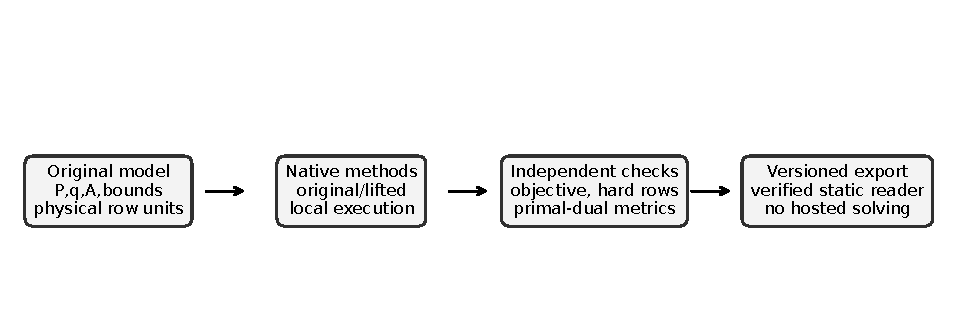
\includegraphics[width=.94\textwidth]{figures/architecture.pdf}
\caption{Implemented data flow from original physical model through native solving and independent acceptance to a versioned static reader. This is an architecture diagram, not a measured speed or reliability result.}\label{fig:architecture}
\end{figure}


The first processing stage constructs or ingests a canonical original-space
problem and physical row descriptions. Authored scalar and control cases
come from deterministic generators. The source-faithful building adapter
preserves its upstream mixed penalties, while separate constructors identify
authored policy variants. Structural validation checks sparse dimensions,
finite numeric values, interval order, units and hard/soft policy before a
backend is selected. Native method packages are owned by a separate public
engine repository; the product scripts do not hide an unpublished internal
solver distribution.

The method stage applies an explicit compatibility rule and runs an admitted
objective using fixed settings. It records available, incompatible and failed
outcomes with reasons. Prepared workspaces retain only the structure their
interface permits, including matrix patterns, coefficients and hard masks.
The evaluation stage recovers original coordinates, objective components,
lower/upper departures and hard error; grouped repeated operations additionally
retain framewise primal and dual checks. This order prevents a library success
flag from being exported as scientific acceptance before original quantities
have been checked.

The export stage validates the scientific documents against their schemas,
writes exact finite UTF-8 data, and produces checksummed inventories and
deployment manifests. Readiness is calculated from actual files and contract
states. JSONL preserves nested diagnostics and unsuccessful observations;
CSV provides a projection for inspection. The static frontend verifies byte
identities and schema/cross-field constraints before rendering a selected case
or an experimental comparison. Its unit filter avoids combining physically
incommensurable departures in one raw numerical axis.

The local cost editor creates a bounded request against a canonical digest.
The user explicitly runs the native scientific command outside the browser
and imports its result envelope. The reader checks that the request, model,
prices, hard policy and recovered metrics agree. Canonical replay and local
native imports receive different provenance labels. A selected C12 stream
cannot be reused after a local policy edit because its stored inputs no
longer match the edited model. The optional API remains a dormant file-serving
component rather than an optimization endpoint.

The grouped research and teaching profiles are separate from the ordinary
public-SDK profile. Their batches, observations and split summaries have
schemas and complete external evidence, but no installed browser replay
adapter. The teaching worker uses direct external CPython, a public SDK
fingerprint and bounded process cleanup. These boundaries permit actual
native methods to be taught without claiming that their external execution
has become a browser capability. No training or fitted model stage exists:
the implemented methods are deterministic optimization procedures, and the
unavailable learned FlexQP policy is not replaced by a fabricated checkpoint.

The distributed application has six scientific routes, but route count is
not a proxy for numerical depth. Scientific authority resides in the exact
inputs, implementations, protocols and accepted outputs. The deployment
workflow builds committed evidence and checks its own commit identity; it
does not regenerate an experimental study to refresh a version badge. This
architecture enables reproducible inspection while retaining the limits of
synthetic data and externally executed numerical work.

\section{Methods}\label{sec:methods}
The executable set contains seven mathematical or implementation paths. Each
description states the objective that the path preserves, its principal numerical
operation, its supported domain and the evidence needed to accept its output.
The comparisons use the same original-space evaluator. Backend status integers
are translated individually; they are not treated as interchangeable proof of
optimality. Algorithmic complexity descriptions refer to identified operations,
not to a measured asymptotic law inferred from a small runtime plot.

\subsection{Explicit slack lifting with OSQP}\label{sec:lift}
Explicit lifting converts a priced interval problem into an ordinary quadratic
program by exposing finite-side departures as optimization variables. For each
soft lower side introduce $t_{L,i}\geq0$, and for each soft upper side introduce
$t_{U,i}\geq0$. Retain original hard rows without slack. The transformed bounds
are
\begin{equation}\label{eq:lift-constraints}
 A_i x+t_{L,i}\geq\ell_i,\qquad A_i x-t_{U,i}\leq u_i,
 \qquad t_{L,i},t_{U,i}\geq0.
\end{equation}
The lifted objective is
\begin{equation}\label{eq:lift-objective}
 \tfrac12x^\top P x+q^\top x+
 \sum_i\left(a_{L,i}t_{L,i}+\tfrac12 b_{L,i}t_{L,i}^2
             +a_{U,i}t_{U,i}+\tfrac12 b_{U,i}t_{U,i}^2\right).
\end{equation}
Monotonicity of the nonnegative side prices permits an optimum whose slacks equal
the actual departures. Zero prices can leave auxiliary variables nonunique, but
recovering departure directly from $Ax$ still gives the correct original
objective. The evaluator therefore does not infer original violation by trusting
an arbitrarily chosen unpriced lifted slack.

The sparse model construction is explicit. Original variables occupy the first
block, followed by only the finite-side auxiliaries actually required. Original
curvature and linear coefficients remain in their block; auxiliary diagonal
curvature and linear prices populate the new entries. Every added nonnegativity
bound and relaxed side has a documented position. This construction supports
side-asymmetric prices without changing their meaning. Compact special helpers
are used for the mixed published building objective, where treating a shared peak
as independent row slacks would instead change the objective.

OSQP applies an operator-splitting iteration to the resulting convex QP and
solves a regularized quasi-definite linear system~\cite{osqp}. Its numerical
regularization is part of the solver subproblem, not an added scientific penalty
in \eqref{eq:lift-objective}. Positive semidefinite problems remain admissible
within the backend's convex domain. Existence of a saddle point and the relevant
fixed or controlled parameter assumptions govern convergence; a finite iteration
limit still produces only the method-specific termination outcome. Numerical
infeasibility certificates and post-solve accuracy checks are separate operations.

Algorithm~\ref{alg:lift} describes the adapter's procedure. After solving, upper-
side lifted multipliers contribute positively to the original row dual and lower-
side multipliers negatively. Hard equalities retain their original dual position.
The resulting $x,y$ are passed to the original objective and feasibility routines.
This recovery makes it possible to compare an enlarged problem to an original-row
implementation without comparing unrelated residual definitions. A small residual
in the lifted coordinates alone would not prove that the right physical model
had been assembled.

\begin{algorithm}[htbp]
\caption{Construct an equivalent finite-side lift, solve its ordinary quadratic program and recover the original-space decision and multiplier for independent evaluation.}\label{alg:lift}
\begin{algorithmic}[1]
\Require Original $P,q,A,\ell,u$, hard mask and side prices
\State Allocate one nonnegative auxiliary for each present soft side
\State Assemble \eqref{eq:lift-constraints} and \eqref{eq:lift-objective}; retain hard rows
\State Solve with the pinned OSQP implementation and explicit settings
\State Recover $x$ and $y_i=y_{U,i}-y_{L,i}$, preserving hard-row multipliers
\State Recompute original objective, departures and raw hard violation
\State Return the backend status and independent metrics, including failure reasons
\end{algorithmic}
\end{algorithm}

The formulation cost depends on the number of finite soft sides and the sparsity
of their incidence. It increases variable and row counts, but that increase does
not determine factorization fill or end-to-end runtime. Sparse ordering, diagonal
structure and reuse of prepared workspaces can make an enlarged problem highly
competitive. For C01 the stored assembled lift has two variables, three rows and
seven nonzeros; the original-row representation has one variable, one row and two
nonzeros. These counts describe assembled matrices, not the nonzeros of a numeric
factor or a guarantee of a particular runtime ratio.

Two uses of lifting must be distinguished. The timed original comparison uses
the pinned native backend for both ordinary lifting and the candidate so backend
implementation differences do not automatically favor one path. The independent
high-accuracy reference uses stock OSQP with tighter tolerances. That reference
is an accuracy oracle, not a timed participant substituted after seeing results.
The coupled comparison separately uses the exact compact peak epigraph. Its
different auxiliary structure is described with the directional method rather
than conflated with independent per-side lifting.

The lift's auxiliary uniqueness deserves particular care in validation. A
strictly positive quadratic departure price determines a unique optimal slack
for a fixed original decision. A zero-price side can instead permit many
auxiliary values with the same scientific cost. Comparing those auxiliaries
componentwise to one reference would reject mathematically equivalent answers.
The evaluator therefore reconstructs the smallest physical departures from
the original row values, retains hard feasibility, and compares the original
objective. This convention also prevents a backend's slack-storage sign from
being mistaken for a physical lower or upper violation in the user-facing
record.

\subsection{Published generalized slack projection}\label{sec:gsp}
Generalized slack projection removes certain explicit slack variables from an
OSQP-style split by replacing the box projection with a proximal operation. The
published derivation and native implementation are due to Schwan, Lew and
Plancher, building on slack elimination in ADMM~\cite{gsp,lew}. The implementation
here preserves the authors' source identity and supported penalty families. It
does not equate a citation to an executed method: compatible synthetic cases
actually call the native backend and recover original-space objectives and duals.

Let $C$ be the row interval box, $\Pi_C$ its projection, and $\Phi$ the supported
slack penalty. The key residual/projection construction is
\begin{equation}\label{eq:gsp-residual}
 R_C(v)=v-\Pi_C(v),\qquad
 T(v)=\Pi_C(v)+\prox_{\Phi/\rho}\bigl(R_C(v)\bigr),\quad \rho>0,
\end{equation}
with the corrective-slack versus violation-residual convention fixed consistently.
The proximal operation itself is
\begin{equation}\label{eq:gsp-prox}
 \prox_{\Phi/\rho}(r)=\argmin_w\left\{\Phi(w)+\tfrac\rho2\|w-r\|_2^2\right\}.
\end{equation}
For the published unconditional penalties, sign symmetry and contraction behavior
permit the generalized projection to represent the eliminated slack problem.
These are mathematical assumptions, not implementation options that can be
ignored when a requested lower price differs from an upper price.

The supported published paths include symmetric quadratic, linear, elastic and
selected Huber or grouped penalties. In C13 the mixed objective exercises that
broader native penalty representation. By contrast, the authored side-asymmetric
energy variants cannot be sent to this backend as if their coefficients were
symmetric. The adapter returns an incompatible state with a reason rather than
averaging the coefficients or solving a symmetric surrogate. This refusal is
visible in both the method inventory and the cross-case displays.

The modified proximal operation changes the row update without necessarily
enlarging the original $x,z$ principal system. That property is useful when a
problem repeatedly updates its vectors while retaining matrices and penalty
structure. It does not remove the sparse system solve, guarantee invariant fill,
or imply that every numerical parameter change is free. An adaptive ADMM penalty
can require refactorization even when the matrix dimensions remain identical.
The computational comparison consequently measures the complete specified
operation rather than counting auxiliaries as a substitute for elapsed time.

Algorithm~\ref{alg:gsp} separates compatibility, numerical execution and original
acceptance. A prepared workspace may retain fixed matrices, a fixed hard mask,
the finite-side pattern and the admitted penalty family. Only permitted vector
changes are applied during repeated execution. Passing a different group layout
or a different coefficient structure is not a valid vector-only update. The
same restrictions apply to references and the candidate, avoiding a comparison
that grants reuse only to one selected implementation.

\begin{algorithm}[htbp]
\caption{Execute the published generalized projection only on supported penalty semantics, retaining the original row system and independent objective and feasibility recovery.}\label{alg:gsp}
\begin{algorithmic}[1]
\Require Original problem, published penalty family and pinned backend
\State Check symmetry, grouping and finite-side assumptions
\If{the requested objective is unsupported}
\State Return incompatible with the precise semantic reason
\EndIf
\State Prepare the original-row linear system and admitted penalty descriptors
\State Iterate the native solve and generalized row operation \eqref{eq:gsp-residual}
\State Recover original $x,y$; evaluate the requested original objective
\State Report termination, hard violation, disagreement and numerical diagnostics
\end{algorithmic}
\end{algorithm}

Convergence follows the underlying convex splitting result only within its
stated assumptions, including appropriate solution existence and numerical
parameter conditions~\cite{admm,eckstein}. The published proximal formula is not
a blanket theorem for a sign-asymmetric, variable-metric or learned-parameter
extension. The separate candidate derivations state precisely which broader
penalties and fixed metrics are considered. Their accuracy and convergence
claims do not retroactively enlarge the domain of the authors' code.

Source attribution is substantive. The adapted native code is distributed by
the separate engine; nested OSQP and QDLDL terms are retained alongside the
OSQPSlack notice. The building source is reproduced with its original mixed
penalties before authored variants are introduced. Preserving those distinctions
allows a reader to identify what is reproduced, what is an adapter, and what is
a mathematical extension. A plot that omits incompatible cells must retain their
reasons elsewhere; otherwise absence can be mistaken for a successful zero-cost
solution or evidence that a supported reference was never executed.

The common projection notation does not erase differences between separable
and shared-group costs. With independent quadratic prices, each row operation
can be evaluated separately. A shared infinity-norm price requires a joint
operation because changing one row's largest departure can alter the group's
active coordinates. The published native descriptors encode that grouping.
The source-faithful building case exercises precisely this distinction. A
consumer that merely checks the number of rows, while dropping the group
descriptor, could accept a well-formed numerical vector for the wrong
optimization problem. Original objective reconstruction is therefore part
of the reference comparison, not an optional display calculation.

\subsection{DAQP with side-specific elastic weights}\label{sec:daqp}
DAQP uses a dual active-set strategy for convex quadratic programs and exposes
side-specific soft weights through its public interface~\cite{daqp,goldfarb}.
This capability is important to the comparison: asymmetry alone cannot be
claimed as a new modeling feature of an original-row projection method. A fair
adapter must reproduce the requested finite objective rather than select the
backend's default softness convention and call the result equivalent.

For a compatible elastic side with departure $t\geq0$, the requested price is
\begin{equation}\label{eq:daqp-cost}
 \varphi(t)=a t+\tfrac12 b t^2,\qquad a\geq0,\quad b>0.
\end{equation}
The adapter maps the quadratic convention reciprocally where the public
backend defines a softness parameter through its inverse curvature. The precise
mapping is applied per side, with lower and upper coefficients kept separate.
It is validated by evaluating \eqref{eq:daqp-cost} in original coordinates after
the solve, rather than assuming that similarly named interface fields have the
same units or normalization. Dividing by a zero quadratic price is not a valid
way to request a pure linear objective.

An active set identifies constraints whose multipliers may be nonzero. For a
positive-definite original Hessian, eliminating the primal vector yields a dual
quadratic structure involving
\begin{equation}\label{eq:daqp-dual}
 x=-P^{-1}(q+A^\top y),\qquad
 A P^{-1}A^\top,
\end{equation}
with the finite-side and elastic conventions handled by the backend. This
identity explains why positive-definite curvature matters to the direct path;
it is not a prescription to form dense inverses explicitly. The tested adapter
uses the library interface and its maintained factors. It does not repair a
semidefinite scientific model by adding an undisclosed Hessian shift.

The ordinary comparison admits DAQP when the base Hessian and finite soft-side
quadratic coefficients meet the implemented positive-definite elastic domain.
Pure L1 and grouped/Huber objectives are incompatible with that particular
mapping. The coupled study has separately registered direct epigraph and
proximal DAQP policies, including their stated linear-programming cases. Those
policies are not silently substituted into the earlier experiment. Distinct
protocols make their different acceptance and termination conditions inspectable.

Algorithm~\ref{alg:daqp} describes the direct side-weight adapter. The conversion
has explicit size bounds of 2048 variables and 8192 finite sides or rows where
applicable. These are implementation resource limits, not mathematical
restrictions of convex quadratic programming. A refusal at this boundary is
retained as an unavailable operation; it does not justify reporting a successful
answer to a smaller or differently regularized model. Inputs that pass the size
check still require semantic compatibility and original-space evaluation.

\begin{algorithm}[htbp]
\caption{Map compatible side-specific elastic prices into DAQP, retain its active workspace for allowed vector updates and recover original-space objective and multipliers.}\label{alg:daqp}
\begin{algorithmic}[1]
\Require Positive-definite admitted QP and finite-side elastic coefficients
\State Check finite dimensions, hard mask, side pattern and strictly positive quadratic prices
\State Convert each lower and upper softness convention with its physical scale
\State Prepare DAQP; retain factor and active state for compatible vector updates
\State Solve; interpret the backend's own status convention
\State Recover original dual signs and independently evaluate all original rows
\State Return accepted only if the external accuracy requirements also hold
\end{algorithmic}
\end{algorithm}

Repeated-operation fairness requires using DAQP's documented update operation.
The prepared workspace preserves its active state and updates only the allowed
linear term and bounds. It does not resend a complete sense vector on every
frame when the public API already permits a cheaper vector update. Conversely,
changing penalty structure invalidates that reuse. The measured timing includes
the selected preparation/update boundary consistently, so the comparison is not
an active-set warm start against a deliberately rebuilt reference.

Backend status interpretation is method-specific. DAQP's status indicating a
soft optimum cannot be read using OSQP's integer convention, where a numerically
equal value may denote an inaccurate result. The adapter translates the status,
then recomputes objective discrepancy and maximum raw hard violation. In the
coupled study, candidate vectors also face the separate primal and dual checks.
An active-set result that is fast but solves the wrong softness scaling is
therefore rejected; a correct result outside the supported direct domain is not
manufactured by altering the objective. These controls preserve the scientific
comparison even when different backends make different engineering tradeoffs.
The separately registered proximal DAQP policies address additional epigraph
regimes through a proximal-point interpretation rather than a permanent
scientific Hessian shift~\cite{daqpprox,rockafellarppa}. Their original objective
is checked after numerical recovery. This distinction matters for a zero-
Hessian linear-price case: a positive quadratic term introduced only to
make a direct solver callable would change the requested model. The protocol
instead admits only its explicitly specified policies and retains unsupported
or unsuccessful outcomes. These later grouped policies do not retroactively
expand the direct adapter's compatibility in the original separable timing
study, whose method settings and excluded cells remain fixed.

\subsection{Fixed-parameter FlexQP reconstruction}\label{sec:flex}
FlexQP addresses elastic quadratic optimization with a splitting formulation;
Deep FlexQP additionally uses a learned numerical-parameter policy~\cite{flex}.
The implemented reference reconstructs the fixed equations and Algorithm~1 from
the paper. It is neither the authors' released implementation nor a reproduction
of a learned policy. Trained weights, training data and a reproducible policy
implementation were unavailable within the comparison. The fixed reconstruction
is nevertheless executable on its stated domain and is evaluated against the
same independent lifted original objective.

The admitted model has positive finite-side linear prices and no finite hard
rows or quadratic soft costs. After converting finite sides to inequalities,
the elastic problem can be written as
\begin{equation}\label{eq:flex-model}
 \min_{x,s\geq0}\ \tfrac12x^\top P x+q^\top x+w^\top s
 \quad\text{subject to}\quad Gx-s\leq h,\qquad w>0.
\end{equation}
Lower interval sides become signed inequalities with their own prices. This
conversion preserves directionality, but it does not justify giving a hard
physical row a finite weight. The adapter consequently refuses hard rows rather
than choosing a numerically large weight and calling it exact hardness.

The fixed numerical parameters are $\sigma_x=10^{-6}$, $\sigma_s=1$, $\rho=1$
and relaxation $\alpha=1.6$. Eliminating the slack-related block produces the
Schur system
\begin{equation}\label{eq:flex-system}
 K=P+\sigma_x I+cG^\top G,\qquad
 c=(\sigma_s^{-1}+\rho^{-1})^{-1}.
\end{equation}
The positive proximal terms stabilize the numerical subproblem. They do not
modify the scientific objective in \eqref{eq:flex-model}; treating $\sigma_x$
as an objective regularizer would change the target optimizer. This distinction
is checked through original objective evaluation and stationarity, not through
a comparison of the stabilized subproblem's objective.

The implementation uses Python and SciPy iteration around its prepared factors.
It is less mature and has different language-level overhead from the compiled
C backends. Observed runtime differences therefore measure these concrete
implementations under the protocol, rather than an implementation-independent
lower bound on the FlexQP formulation. The reconstruction is not retuned after
examining the held-out results. In particular, the comparison does not choose a
different proximal parameter for each unfavorable test instance.

Algorithm~\ref{alg:flex} states the executable boundary without conflating
fixed and learned variants. The original dual of \eqref{eq:flex-model} has
finite-side bounds determined by the linear prices. The implementation checks
stationarity and the projected dual-box residual rather than accepting only a
small change between successive iterates. A stable iteration can converge to
the wrong fixed point if the sign or price mapping is incorrect; original-space
conditions are needed to distinguish that defect from a genuinely small step.

\begin{algorithm}[htbp]
\caption{Execute the fixed FlexQP equations on an admitted pure linear elastic problem, preserving original prices and independently testing the returned original-space optimum.}\label{alg:flex}
\begin{algorithmic}[1]
\Require Compatible pure linear elastic inequalities and fixed numerical parameters
\State Refuse finite hard rows, quadratic prices and nonpositive admitted side prices
\State Convert finite interval sides into $Gx-s\leq h$ with original linear prices
\State Prepare \eqref{eq:flex-system} using the fixed proximal parameters
\State Iterate the paper's fixed splitting and relaxation updates
\State Check original stationarity and projected dual-box residuals
\State Recover interval dual signs and compare the original objective to lifting
\end{algorithmic}
\end{algorithm}

The relationship between a finite elastic optimum and hard feasibility requires
care. If the original hard inequalities are feasible and suitable multiplier
bounds are known, a sufficiently large exact linear price can recover a hard
solution. That result does not make every finite price exact, nor does it make
the output safe for a plant whose immutable limits have been softened. The
application explicitly describes the objective being priced and separates it
from the original hard mask. This is a modeling and acceptance requirement,
not a criticism unique to one elastic algorithm.

Compatibility exclusions remain part of the scientific denominator. Symmetric
and asymmetric elastic families with nonzero quadratic side prices are outside
this pure linear reconstruction. They are marked incompatible before timing,
not counted as inaccurate solves or assigned zero durations. Conversely,
admitted asymmetric linear cases are genuinely executed and checked, so an
unavailable learned policy is not used to excuse omission of the fixed published
reference. The complete six-path original comparison can therefore expose
both semantic limits and implementation costs without pretending that all
methods solve every penalty family.
Within a prepared fixed-policy operation, the signed inequality matrix and
its numerical factor can be retained while admitted vectors change. A new
hard mask, finite-side pattern or price structure is not such a vector
change. The reconstruction's boundary checks distinguish these cases before
reuse. This is also why the complete-call timing is more informative than
an isolated triangular solve: it includes the work required to admit and
recover the actual scientific problem. The theoretical proximal regularizers
and the practical implementation overhead must both remain visible when
interpreting a comparison with a mature compiled backend.

\subsection{ElastiQP for pure linear elastic inequalities}\label{sec:elasti}
ElastiQP provides a published dual active-set solver for elastic quadratic
problems motivated by constrained robot control~\cite{elasti}. The product
consumes its pinned public version~0.2.0 implementation as a separate comparison path.
Its supported domain is not identified merely by the word elastic. The adapter
admits positive-definite base curvature, pure linear finite-side prices, and
hard equalities. It refuses quadratic side prices and hard inequalities that
the implemented interface cannot preserve exactly.

After finite-side conversion, the mathematical problem is
\begin{equation}\label{eq:elasti-model}
 \min_x\ \tfrac12x^\top P x+q^\top x+
             \sum_j w_j(G_jx-h_j)_+
 \quad\text{subject to}\quad Ex=e,\qquad P\succ0,\quad w_j>0.
\end{equation}
A lower interval side becomes the signed row $-A_i x\leq-\ell_i$ with its
lower-side price. An upper side retains $A_i x\leq u_i$ and its upper-side
price. Equality rows are placed in $E$, rather than replaced by two finite
linear penalties. This construction makes the physical hard/soft distinction
recoverable after solving.

The elastic inequality multipliers lie in a bounded dual box. Conditional on
an active dual configuration, the primal/equality calculation satisfies
\begin{equation}\label{eq:elasti-kkt}
 \begin{bmatrix}P&E^\top\\E&0\end{bmatrix}
 \begin{bmatrix}x\\\nu\end{bmatrix}
 =\begin{bmatrix}-q-G^\top\mu\\e\end{bmatrix},
 \qquad 0\leq\mu\leq w.
\end{equation}
The expression explains the distinction between capped elastic multipliers
and equality multipliers; it is not an instruction to build or invert this
matrix independently of the library. The backend maintains the numerical
structures appropriate to its algorithm. The adapter's task is to preserve the
input model and recover the original coordinates and signs.

Algorithm~\ref{alg:elasti} describes that boundary. In particular, a backend
termination flag is interpreted using ElastiQP's own convention before the
external evaluator recomputes the requested objective. Positive-definite
curvature is checked rather than created through an undisclosed Hessian shift.
A problem whose optimum is changed by a small regularizer is not a matched
reference, even if the regularizer seems numerically harmless in a particular
example. Likewise, a hard inequality is not silently converted to a costly
elastic preference just because the original hard model is feasible.

\begin{algorithm}[htbp]
\caption{Preserve admitted pure linear interval prices and hard equalities in ElastiQP, then recover original row multipliers and independently evaluate the scientific objective.}\label{alg:elasti}
\begin{algorithmic}[1]
\Require Positive-definite original model with admitted pure linear soft sides
\State Refuse quadratic prices, unsupported hard inequalities and conversion limits
\State Form signed finite-side inequalities and retain hard equalities separately
\State Call the pinned ElastiQP implementation with explicit numerical settings
\State Recover $x$, finite-side multipliers and hard-equality multipliers
\State Combine lower and upper multipliers in original row order
\State Evaluate original objective, raw hard violation and oracle discrepancy
\end{algorithmic}
\end{algorithm}

The conversion shares explicit implementation limits with the other dense
reference adapters: admitted dimensions are bounded before numerical allocation.
These limits are recorded as resource restrictions and do not imply that larger
mathematical problems are ill-defined. Memory behavior depends on the converted
finite-side count, equality structure and maintained active-set data. A runtime
comparison must therefore preserve the conversion cost and the chosen timing
boundary. Comparing only a selected inner iteration to another backend's full
validation/export call would answer a different question.

The published always-feasible elastic formulation concerns feasibility of the
relaxed optimization representation. It does not mean every original operating
inequality holds at a finite-price optimum. For example, if satisfying a comfort
limit costs more in the base objective than the declared linear departure price,
the optimizer may purchase a violation. Hard equality satisfaction remains a
separate requirement. The application displays raw departure and hard-error
quantities so an elastic status is not mistaken for a certificate of physical
admissibility.

In the original synthetic timing study, the pure linear family is the natural
compatible domain for this reference. The quadratic elastic families remain
incompatible rather than being rerun with their quadratic coefficient removed.
This produces a heterogeneous but explicit method-case matrix. The comparison
does not infer that one reference is universally stronger from a count of
compatible cells; each compatibility rule follows the actual represented
objective. The data retain excluded cells, backend failures and accuracy checks
as different states, enabling a reader to determine whether an apparent runtime
difference is numerical or simply a change in the problem being solved.
The bounded elastic dual also explains a common modeling mistake. Reaching
the upper multiplier price cap can be consistent with a positive departure
at the optimum; it is not necessarily a failed active-set calculation.
The price cap belongs to the chosen objective. Equality multipliers are
not capped by that same finite-side price, because their constraints remain
hard. Recovering those two multiplier classes separately prevents an apparently
small aggregate residual from concealing softened dynamics. The exported
original-space state therefore records policy, objective and feasibility
together rather than presenting one generic elastic success label.

\subsection{Side-specific interval proximal update}\label{sec:asymmetric}
The side-specific projection path evaluates the separable penalty
\eqref{eq:side-price} inside an original-row OSQP-style iteration. Its narrow
implementation property is that lower and upper linear/quadratic coefficients
enter the row operation without adding independent departure variables to the
principal system. Unequal side costs already have established formulations,
including the DAQP interface. The question tested by the original experiment
is computational cost against equivalent lifting, not whether unequal prices
can be modeled for the first time.

For a temporary scalar value $v$ and positive numerical metric $\rho$, the row
operation solves
\begin{equation}\label{eq:asym-subproblem}
 z^+=\argmin_z\{g_i(z)+\tfrac\rho2(z-v)^2\}.
\end{equation}
It has the closed form
\begin{equation}\label{eq:asym-prox}
z^+=\begin{cases}
\ell_i-\dfrac{[\rho(\ell_i-v)-a_{L,i}]_+}{\rho+b_{L,i}},&v<\ell_i,\\[5pt]
v,&\ell_i\leq v\leq u_i,\\[3pt]
u_i+\dfrac{[\rho(v-u_i)-a_{U,i}]_+}{\rho+b_{U,i}},&v>u_i.
\end{cases}
\end{equation}
An absent side is omitted. A hard row uses exact interval projection. The
positive denominator follows from $\rho>0$ and nonnegative quadratic price;
the formula remains defined for a pure linear or a zero-price soft side.

To derive the upper branch, write $d=z-u_i>0$. Differentiating the exterior
quadratic yields $(\rho+b_{U,i})d=\rho(v-u_i)-a_{U,i}$. If its right-hand side
is nonpositive, the exterior optimum is inadmissible and the endpoint satisfies
the subgradient condition. Otherwise division gives the positive departure.
The lower branch follows by reflecting the displacement and using the lower
coefficients. Inside the interval the price is zero and $z=v$ minimizes the
proximal displacement. Strong convexity of \eqref{eq:asym-subproblem} establishes
uniqueness, including at the interval endpoints.

This scalar derivation is an application of established proximal convex
analysis~\cite{prox,moreau,rockafellarppa}. It is not a proof of arbitrary adaptive
ADMM behavior, a finite-precision error theorem or a global priority claim.
Within a fixed positive metric and an attained primal and dual solution, the
underlying splitting framework supplies the relevant convergence argument.
Unit conversion must transform the side prices, row coefficients and dual
coordinates consistently. A positive absolute tolerance in physical departure
units cannot by itself establish covariance across metres and centimetres.

Algorithm~\ref{alg:asym} identifies the actual native procedure. The separate
engine owns the C/C++ update, Python bindings, scaling and objective recovery.
The product consumes the public SDK in an isolated profile. Grouped and Huber
costs do not become supported merely because their scalar notation resembles
an elastic price. The separable adapter refuses them; the mixed C13 model uses
the published generalized projection or exact lifting instead.

\begin{algorithm}[htbp]
\caption{Apply side-specific scalar proximal updates in the original interval rows while preserving hard policy and independently recovering the requested objective and dual conditions.}\label{alg:asym}
\begin{algorithmic}[1]
\Require Admitted separable original problem, side prices and positive row metric
\State Prepare the fixed-shape original-row native workspace
\For{each row-update operation}
\State Project hard rows; apply \eqref{eq:asym-prox} to each admitted soft row
\State Continue the native primal/dual splitting update
\EndFor
\State Recover original $x,y$ and physical lower/upper departures
\State Evaluate the original objective and method-specific termination criteria
\State Compare accepted outputs to the independent equivalent lift
\end{algorithmic}
\end{algorithm}

The implementation must preserve more than the scalar minimizer. Original
objective evaluation, the dual conjugate, scaling, recession behavior and
fixed-shape repeated updates have independent controls. A stationary vector
can still violate the soft subgradient relation. The diagnostic proximal test
$z=\prox_g^{H_0}(z+H_0^{-1}y)$ checks that relation at the original row value rather than
selecting a derivative arbitrarily at a kink. Here $H_0$ is an explicitly
positive diagonal diagnostic metric; its numeric identity applies only in
canonical diagnostic coordinates. Signed slack cancellation is
prevented by separate lower and upper departure arrays.

The original held-out endpoint does not establish the registered computational
gain. Its median relative reduction is \OriginalEstimate\%, with a confidence
interval crossing zero. Correctness and retained original dimensions therefore
coexist with a negative timing conclusion. A favorable selected family, one
small scalar matrix or a quick warm update cannot replace that primary result.
The implementation remains a complete executable method within its supported
domain; its scientific limitations are stated through the full comparison,
not hidden by relabeling the failed prediction as a different acceptance rule.
Endpoint behavior supplies useful concrete controls. A sufficiently large
linear price relative to one temporary proximal displacement maps that
displacement exactly to the preferred endpoint. This is a statement about
one proximal subproblem, not a guarantee that a finite price enforces the
original row for every possible model or iteration. Setting the quadratic
price to zero leaves a genuine one-sided soft-threshold operation. Setting
both prices to zero leaves a free preference, while an explicit hard mask
still projects exactly. Confusing these three cases changes the optimization
policy even though each resulting program can remain convex and solvable.
The scalar analytic cases and independently recovered original dual signs
test these distinctions without relying on matching backend status integers
or comparing an auxiliary representation to itself.

\subsection{Directional disjoint group-peak proximal update}\label{sec:directional}
The second proximal path prices the largest weighted departure within each
disjoint group, using \eqref{eq:group-peak}. It permits unequal upper and lower
scales and keeps the original interval-row representation in its principal
system. Existing directional row splitting and compact epigraphs express the
same objective, so row preservation is a representation property rather than
an expressibility or priority result. Coordinatewise orthant monotonicity and
weighted threshold calculations have established antecedents~\cite{orthant,weighted}.

For a box $C$ and residual penalty $\Psi$, assume $\Psi$ is proper, closed,
convex, nonnegative, minimized at zero, and nonincreasing under coordinate
contractions $D=\diag(d_i)$ with $0\leq d_i\leq1$. For fixed diagonal $H\succ0$,
the exact identity is
\begin{equation}\label{eq:directional-prox}
 \prox_{g_C}^{H}(v)=\Pi_C(v)+\prox_{\Psi}^{H}(v-\Pi_C(v)),\qquad
 g_C(z)=\inf_{s\in C}\Psi(z-s).
\end{equation}
The proof clips each candidate to the coordinate segments between $\Pi_C(v)$
and $v$. Both diagonal quadratic distance and the contraction-monotone penalty
cannot increase. On those segments the problem is exactly the residual
proximal problem. A dense positive metric does not support that coordinatewise
argument; the theorem is not silently extended to arbitrary metric coupling.

For one directional group let $r=v-\Pi_C(v)$, choosing $c_i$ from the active
sign of each residual. A fixed candidate peak $t\geq0$ gives
\begin{equation}\label{eq:directional-clipping}
 w_i(t)=\operatorname{sign}(r_i)\min\{|r_i|,t/c_i\},\qquad
 F(t)=at+\tfrac12bt^2+\tfrac12\sum_i h_i(|r_i|-t/c_i)_+^2.
\end{equation}
Sort the breakpoints $c_i|r_i|$ in descending order and examine a consistent active prefix $S$.
Within that interval, a stationary threshold satisfies
\begin{equation}\label{eq:directional-threshold}
 t=\frac{\sum_{i\in S}h_i|r_i|/c_i-a}
          {b+\sum_{i\in S}h_i/c_i^2}.
\end{equation}
The zero endpoint and empty active set are handled explicitly. If both prices
vanish, the residual is returned unchanged; no zero denominator is evaluated.
Sorting costs $O(k\log k)$ for a group of $k$ rows, followed by a prefix scan.
This extra proximal work can outweigh savings from a smaller principal system.

Algorithm~\ref{alg:directional} states the native operation. The local code
refuses nonrepresentable arithmetic and uses local floating-point spacing at
threshold boundaries. That treatment is important for row-scale covariance:
a fixed absolute floor in departure units would change its meaning under a
reciprocal scale transformation. Group membership remains disjoint in the
implemented interface. Overlapping groups would require a different proximal
calculation and are rejected rather than approximated as independent groups.

\begin{algorithm}[htbp]
\caption{Compute an exact directional group proximal operation in a fixed positive diagonal metric, with explicit free-price, threshold-endpoint and representability handling.}\label{alg:directional}
\begin{algorithmic}[1]
\Require Nonempty admitted interval box, disjoint groups and positive directional scales
\State Compute $p=\Pi_C(v)$ and $r=v-p$; retain hard rows separately
\For{each soft group}
\If{$a=b=0$}\State Keep the residual unchanged
\Else
\State Sort the finite breakpoints $c_i|r_i|$ in descending order
\State Find the consistent threshold interval using \eqref{eq:directional-threshold} and $t=0$
\State Set the residual coordinates using \eqref{eq:directional-clipping}
\EndIf
\EndFor
\State Return $p+w$ and continue fixed-metric relaxed splitting
\end{algorithmic}
\end{algorithm}

The joint dual condition differs from independent coordinate price caps. The
directional dual quantity is a sum of positive and negative multiplier parts
divided by their corresponding scales. Its conjugate yields one group budget.
The evaluator therefore checks every group's normalized Fenchel relation and
every hard row's complementarity separately, alongside stationarity and bounded
dual repair. A signed aggregate gap is retained diagnostically but cannot
allow an erroneous soft subgradient to cancel a negative hard-row gap.

The fixed-metric relaxation scope is $0<\alpha<2$ with the stated convexity
and attained-saddle-point assumptions. No variable-metric or arbitrary adaptive-
relaxation theorem is claimed. The complete repeated-forecast comparison uses
public SDK 0.2 and includes matched row-split, compact epigraph and direct/proximal
DAQP policies. Its primary score is \PrimaryEstimate\%, including all failed
pairs under the prespecified rule. That result refutes the registered timing
prediction on the tested population. It cannot be converted to a uniform
slowdown multiplier, nor rescued by omitting oracle limits, unsuccessful native
operations or semantically incompatible reference cells.
The physical scale controls also separate two superficially similar edits.
Multiplying an original row and its bounds by a positive conversion factor,
while dividing both directional scales by that factor, preserves the peak
and physical optimizer. Multiplying only the upper directional scale changes
the relative policy price. The teaching example intentionally exercises both
operations and compares actual native, row-split and epigraph answers. Its
hard coupling equality remains exact while the selected physical allocation
can change under the policy edit. This demonstrates the model's semantics;
it is not an additional performance experiment. The same distinction is
enforced in the research batch's unit arrays and source digests so that a
recorded scale conversion cannot silently become a new optimization objective.
Keeping those arrays attached to the original rows is essential when the
reference expands their representation into signed one-sided constraints.
The expanded reference retains a recoverable mapping to each original lower
or upper side, so its dual comparison tests the same physical quantity.


\section{Experimental protocol}\label{sec:protocol}
The teaching catalog, original timing study, repeated-control stream and
grouped repeated-forecast study answer different questions. They are not
pooled into one statistical sample. Catalog cases establish semantic and
numerical examples; the two registered studies test separately specified
computational predictions; the stream describes reuse on a common physical
trajectory. Benchmark methodology requires an explicit problem population,
consistent success criteria and comparable timing boundaries~\cite{dolan,cutest}.
A solver ranking obtained after removing unsupported or unsuccessful cells
would otherwise mix representability, numerical reliability and speed.

The original main grid uses dimensions 32,64,128 and 256, twice as many rows
as variables, densities 0.05 and 0.2, and diagonal Hessian conditions 1 and 1000.
Its three families are symmetric elastic, asymmetric elastic and asymmetric
linear. Development seeds 1000--1002 and evaluation seeds 9000--9005 are
distinct. The 24-instance robustness calculation uses dimension 32, density 0.1,
six additional seeds and conditions 1,100,10000 and 1000000 while keeping the
other generated quantities fixed within each seed. Together these populations
contain 456 instances. Rows are normalized before the declared cost/target
distribution is applied; independent unit and scaling examples are separate
from a claim that this grid covers arbitrary physical row scaling.

Each original backend has one warm-up and seven measured repetitions.
Method order is randomized by the fixed ordering seed within an instance
and repetition. The cold end-to-end boundary includes input validation,
formulation construction, setup, solve and original evaluation. It excludes
generation, module import and export. The primary population is the asymmetric
elastic family with dimension at least 128 and density 0.05. Its 24 distinct
problems and seven repetitions produce 168 paired observations across six
evaluation seed clusters. Calling those 168 observations independent generated
instances would be incorrect. The point estimate is the median paired reduction
\begin{equation}\label{eq:original-score}
 R_j=1-\frac{T_{\mathrm{candidate},j}}
 {\min(T_{\mathrm{lift},j},T_{\mathrm{DAQP},j})},\qquad
 \widehat R=\median_j R_j.
\end{equation}
The stored 95\% interval resamples seed clusters with the fixed 2000-resample
procedure. It is not recomputed for the figures. Cluster resampling preserves
dependence among repeated observations from the same generated seed;
bootstrap accuracy with few clusters remains a limitation~\cite{efron,davison,cameron}.
The prediction requires a reduction of at least 10\% and a lower interval
endpoint above zero, together with complete original-space acceptance.

Original numerical settings are absolute/relative solver tolerances of
$10^{-7}$, an iteration limit of 200000, and adaptive penalty checks at interval 25.
The separate stock lifting oracle uses tolerances of$10^{-9}$. External acceptance
requires normalized objective discrepancy and maximum raw hard-row departure
no larger than$10^{-6}$. Stationarity remains diagnostic in that protocol.
Threading is limited to one BLAS thread; one worker is supervised with a 10 second
trial deadline, a 7200 second total limit and a 4 GiB process-memory limit.
These are protocol settings, not observed per-method resource costs.

The C12 stream contains 32 frames of a horizon 20 double-integrator model with
a 0.2 second physical step. An independent stock-lift oracle drives the common
plant, with velocity impulses at frames 8 and 20. Every method receives the
same physical state. Cold calls include preparation; warm calls record
initial workspace setup separately from validation, vector update, solve
and evaluation. There is one documented observation per frame. The stream
supports descriptive reuse comparisons, not a statistical superiority claim
or a comparison of independently controlled plants.

The grouped study retains 48 development,144 held-out and 18 robustness instances.
Each operation includes preparation/factorization and 32 updates, solves,
physical recovery and independent accuracy checks. Library/process startup
and serialization are excluded symmetrically from the inner timer; all
compiled competitors are preloaded. The outer supervisor still retains
startup, deadlines, process memory and cleanup outcomes. Nine method policies
have one warm-up and three measured repetitions per instance, plus an oracle
observation, yielding 7770 raw and 5670 measured method observations. The primary
population contains all 144 held-out instances and six seed clusters. Its
per-instance score compares the native median with the fastest compatible
registered reference; failed pairs retain the specified score of$-1$.
An absent native median or failed oracle cannot be replaced with a favorable
successful subset. The registered minimum improvement and interval condition
remain false regardless of which descriptive formulation plot is displayed.

\section{Results}\label{sec:results}
The results distinguish exact formulation agreement, availability, numerical
acceptance and elapsed-time inference. Tables~\ref{tab:catalog-1} and
\ref{tab:catalog-2} report every stored case/method outcome, including
incompatible cells. Objectives are compared within one unchanged model;
their numerical values are not ranked across different physical objectives.
Hard errors are evaluated on original rows, and N/A denotes the absence
of a compatible returned objective. The complete six-path timing comparison
and separate nine-policy grouped study have their own larger inventories.
\begin{table}[htbp]\centering\footnotesize
\caption{Complete stored catalog outcomes for the indicated cases and every catalog method. N/A means no compatible returned objective, and hard error is evaluated in original row coordinates.}\label{tab:catalog-1}
\begin{tabularx}{\textwidth}{@{}ll>{\raggedright\arraybackslash}Xrrr@{}}\toprule
Case & Method & State & Objective & Hard error & Gap\\\midrule
C01 & lifted & available & -2.\allowbreak{}98167 & 0 & 0\\
C01 & generalized & available & -2.\allowbreak{}98167 & 0 & 0\\
C01 & asymmetric & available & -2.\allowbreak{}98167 & 0 & 0\\
C01 & daqp & available & -2.\allowbreak{}98167 & 0 & 4.\allowbreak{}44089e-16\\
C02 & lifted & available & -2.\allowbreak{}98167 & 0 & 0\\
C02 & generalized & available & -2.\allowbreak{}98167 & 0 & 0\\
C02 & asymmetric & available & -2.\allowbreak{}98167 & 0 & 0\\
C02 & daqp & available & -2.\allowbreak{}98167 & 0 & 4.\allowbreak{}44089e-16\\
C03 & lifted & available & -2.\allowbreak{}564 & 0 & 0\\
C03 & generalized & incompatible & N/\allowbreak{}A & N/\allowbreak{}A & N/\allowbreak{}A\\
C03 & asymmetric & available & -2.\allowbreak{}564 & 0 & 4.\allowbreak{}44089e-16\\
C03 & daqp & available & -2.\allowbreak{}564 & 0 & 4.\allowbreak{}44089e-16\\
C04 & lifted & available & -4.\allowbreak{}14062 & 7.\allowbreak{}33857e-13 & 0\\
C04 & generalized & incompatible & N/\allowbreak{}A & N/\allowbreak{}A & N/\allowbreak{}A\\
C04 & asymmetric & available & -4.\allowbreak{}14063 & 6.\allowbreak{}95773e-10 & 9.\allowbreak{}57696e-11\\
C04 & daqp & available & -4.\allowbreak{}14062 & 0 & 1.\allowbreak{}01252e-13\\
C05 & lifted & available & -4.\allowbreak{}5 & 0 & 0\\
C05 & generalized & available & -4.\allowbreak{}5 & 0 & 2.\allowbreak{}66454e-15\\
C05 & asymmetric & incompatible & N/\allowbreak{}A & N/\allowbreak{}A & N/\allowbreak{}A\\
C05 & daqp & incompatible & N/\allowbreak{}A & N/\allowbreak{}A & N/\allowbreak{}A\\
C06 & lifted & available & -30.\allowbreak{}6139 & 0 & 0\\
C06 & generalized & incompatible & N/\allowbreak{}A & N/\allowbreak{}A & N/\allowbreak{}A\\
C06 & asymmetric & available & -30.\allowbreak{}6139 & 0 & 3.\allowbreak{}66003e-07\\
C06 & daqp & available & -30.\allowbreak{}6139 & 0 & 8.\allowbreak{}1416e-07\\
C07 & lifted & available & -34.\allowbreak{}5757 & 0 & 0\\
C07 & generalized & incompatible & N/\allowbreak{}A & N/\allowbreak{}A & N/\allowbreak{}A\\
C07 & asymmetric & available & -34.\allowbreak{}5757 & 0 & 1.\allowbreak{}09511e-07\\
C07 & daqp & incompatible & N/\allowbreak{}A & N/\allowbreak{}A & N/\allowbreak{}A\\
C08 & lifted & available & -2.\allowbreak{}64164 & 0 & 0\\
C08 & generalized & incompatible & N/\allowbreak{}A & N/\allowbreak{}A & N/\allowbreak{}A\\
C08 & asymmetric & available & -2.\allowbreak{}64164 & 0 & 1.\allowbreak{}24144e-08\\
C08 & daqp & available & -2.\allowbreak{}64164 & 0 & 1.\allowbreak{}32642e-08\\
\bottomrule\end{tabularx}
\end{table}

\begin{table}[htbp]\centering\footnotesize
\caption{Complete stored catalog outcomes for the indicated cases and every catalog method. N/A means no compatible returned objective, and hard error is evaluated in original row coordinates.}\label{tab:catalog-2}
\begin{tabularx}{\textwidth}{@{}ll>{\raggedright\arraybackslash}Xrrr@{}}\toprule
Case & Method & State & Objective & Hard error & Gap\\\midrule
C09 & lifted & available & -34.\allowbreak{}0702 & 0 & 0\\
C09 & generalized & available & -34.\allowbreak{}0702 & 9.\allowbreak{}42717e-08 & 2.\allowbreak{}83169e-07\\
C09 & asymmetric & available & -34.\allowbreak{}0702 & 9.\allowbreak{}42717e-08 & 2.\allowbreak{}83169e-07\\
C09 & daqp & available & -34.\allowbreak{}0702 & 8.\allowbreak{}88178e-16 & 6.\allowbreak{}51837e-09\\
C10 & lifted & available & -31.\allowbreak{}3247 & 0 & 0\\
C10 & generalized & available & -31.\allowbreak{}3247 & 1.\allowbreak{}82809e-07 & 8.\allowbreak{}24346e-07\\
C10 & asymmetric & available & -31.\allowbreak{}3247 & 1.\allowbreak{}82809e-07 & 8.\allowbreak{}24346e-07\\
C10 & daqp & available & -31.\allowbreak{}3247 & 1.\allowbreak{}77636e-15 & 1.\allowbreak{}03659e-08\\
C11 & lifted & available & 3.\allowbreak{}89929 & 0 & 0\\
C11 & generalized & incompatible & N/\allowbreak{}A & N/\allowbreak{}A & N/\allowbreak{}A\\
C11 & asymmetric & available & 3.\allowbreak{}89929 & 0 & 4.\allowbreak{}44089e-16\\
C11 & daqp & available & 3.\allowbreak{}89929 & 0 & 0\\
C12 & lifted & available & -41.\allowbreak{}204 & 1.\allowbreak{}90152e-10 & 0\\
C12 & generalized & incompatible & N/\allowbreak{}A & N/\allowbreak{}A & N/\allowbreak{}A\\
C12 & asymmetric & available & -41.\allowbreak{}204 & 4.\allowbreak{}21994e-10 & 4.\allowbreak{}61511e-08\\
C12 & daqp & available & -41.\allowbreak{}204 & 8.\allowbreak{}88178e-16 & 6.\allowbreak{}16883e-08\\
C13 & lifted & available & 36.\allowbreak{}6605 & 6.\allowbreak{}53606e-10 & 0\\
C13 & generalized & available & 36.\allowbreak{}6605 & 7.\allowbreak{}52559e-09 & 1.\allowbreak{}61722e-08\\
C13 & asymmetric & incompatible & N/\allowbreak{}A & N/\allowbreak{}A & N/\allowbreak{}A\\
C13 & daqp & incompatible & N/\allowbreak{}A & N/\allowbreak{}A & N/\allowbreak{}A\\
C14 & lifted & available & 48.\allowbreak{}403 & 2.\allowbreak{}37126e-09 & 0\\
C14 & generalized & incompatible & N/\allowbreak{}A & N/\allowbreak{}A & N/\allowbreak{}A\\
C14 & asymmetric & available & 48.\allowbreak{}403 & 2.\allowbreak{}09591e-08 & 2.\allowbreak{}54563e-06\\
C14 & daqp & incompatible & N/\allowbreak{}A & N/\allowbreak{}A & N/\allowbreak{}A\\
C15 & lifted & available & 42.\allowbreak{}6822 & 1.\allowbreak{}43467e-09 & 0\\
C15 & generalized & incompatible & N/\allowbreak{}A & N/\allowbreak{}A & N/\allowbreak{}A\\
C15 & asymmetric & available & 42.\allowbreak{}6822 & 2.\allowbreak{}72591e-09 & 2.\allowbreak{}17369e-06\\
C15 & daqp & incompatible & N/\allowbreak{}A & N/\allowbreak{}A & N/\allowbreak{}A\\
\bottomrule\end{tabularx}
\end{table}


Figure~\ref{fig:scalar-objective} isolates the scalar lower-side example.
The actual exported optima agree on a purchased lower departure rather than
on the preferred interval itself. Its piecewise-quadratic objective curve is an evaluation
of the stored mathematical objective, not an extra numerical experiment.
The shaded interval identifies preference, not a physical hard bound. This
small example illustrates why an elastic optimum can be correct while
violating the preferred row. Figure~\ref{fig:formulation-size} shows the
exported variable counts across all fifteen cases. Larger or smaller principal
formulations do not directly measure factorization fill, cache behavior or
complete-operation cost.
\begin{figure}[htbp]\centering
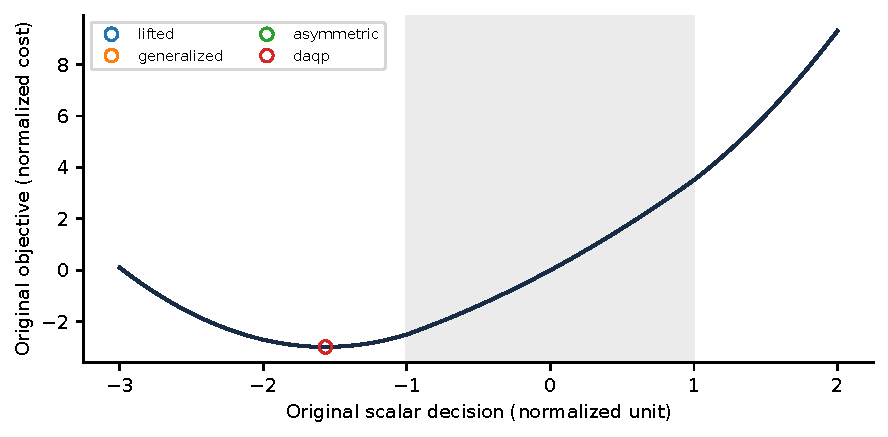
\includegraphics[width=.94\textwidth]{figures/scalar-objective.pdf}
\caption{Analytic evaluation of the stored C01 objective and actual exported method optima. The shaded interval is the preferred band, and the curve is a mathematical illustration rather than a new timed observation.}\label{fig:scalar-objective}
\end{figure}

\begin{figure}[htbp]\centering
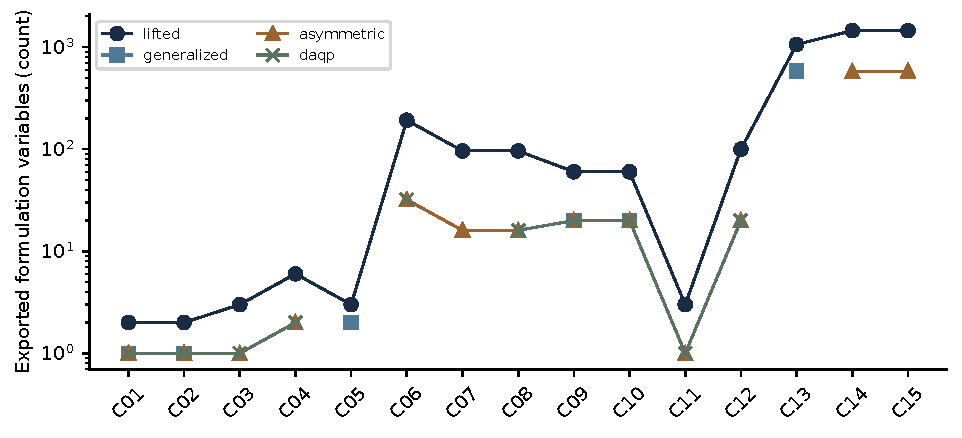
\includegraphics[width=.94\textwidth]{figures/formulation-size.pdf}
\caption{Exported variable counts for all fifteen stored catalog cases and four catalog paths. Missing points denote unsupported objectives; the counts describe formulation size and do not measure factorization fill or computational advantage.}\label{fig:formulation-size}
\end{figure}


Figure~\ref{fig:compatibility} makes the catalog's semantic exclusions explicit.
The source-faithful building objective admits lifting and published generalized
projection while refusing unsupported separable substitutions. The asymmetric
energy variants instead define different prices, so their stored objectives
cannot be read as algorithmic improvements over the mixed-policy optimum.
Likewise, an incompatible symmetric projection on the asymmetric C12 stream
is not a failed numerical solve of the same admitted objective. The matrix
distinguishes these states before any runtime reading is attempted.
\begin{figure}[htbp]\centering
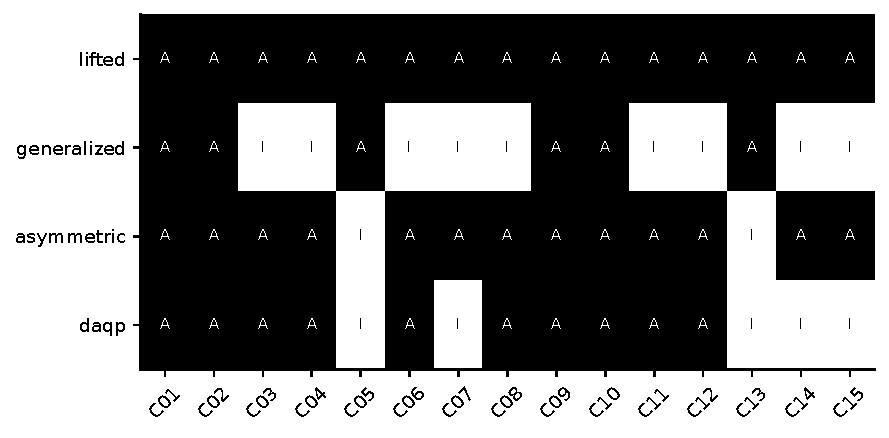
\includegraphics[width=.94\textwidth]{figures/compatibility.pdf}
\caption{Full catalog method-case compatibility: A denotes an available exported solution and I an incompatible requested objective. This four-path catalog is distinct from the six-path original timing study and the separate grouped study.}\label{fig:compatibility}
\end{figure}


The original computation completed all 456 planned instances with 11592 accepted
and 7560 incompatible measured observations and no numerical or external-accuracy
rejection. Table~\ref{tab:main-results} preserves its primary 168 paired
observations and the separate grouped endpoint. The original reduction
\OriginalEstimate\% has a 95\% interval crossing zero. Figure~\ref{fig:original-effect}
therefore does not establish the predicted 10\% gain. The plotted zero and
ten-percent reference lines are inferential context, not replacement cutoffs
chosen after observing the estimate. Figure~\ref{fig:cold-times} shows stored
cell medians and interquartile ranges for one prespecified family/density
slice; that descriptive slice does not replace the full primary analysis.
\begin{table}[htbp]\centering\footnotesize
\caption{Distinct primary populations, stored effect estimates and uncertainty for the two completed timing studies. Failed-pair rules are not transferred between experiments and neither registered ten percent improvement criterion is established.}\label{tab:main-results}
\begin{tabularx}{\textwidth}{@{}>{\raggedright\arraybackslash}Xrrrr@{}}\toprule
Study & Population & Pairs & Effect (\%) & 95\% limits\\\midrule
Separable & 456 & 168 & 0.\allowbreak{}499839 & -3.\allowbreak{}29197, 3.\allowbreak{}94484\\
Grouped & 210 & 144 & -212.\allowbreak{}45 & -225.\allowbreak{}337, -192.\allowbreak{}874\\
\bottomrule\end{tabularx}
\end{table}

\begin{figure}[htbp]\centering
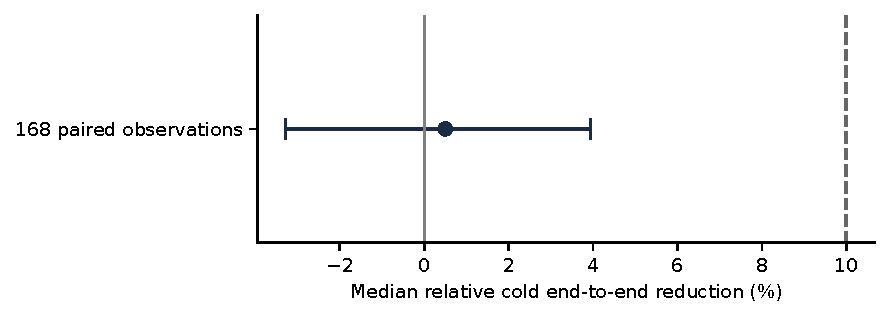
\includegraphics[width=.94\textwidth]{figures/original-effect.pdf}
\caption{Original held-out timing estimate with its stored 95 percent seed-cluster confidence interval and registered ten percent reference. The interval crosses zero; neither interval nor population is recomputed for this figure.}\label{fig:original-effect}
\end{figure}

\begin{figure}[htbp]\centering
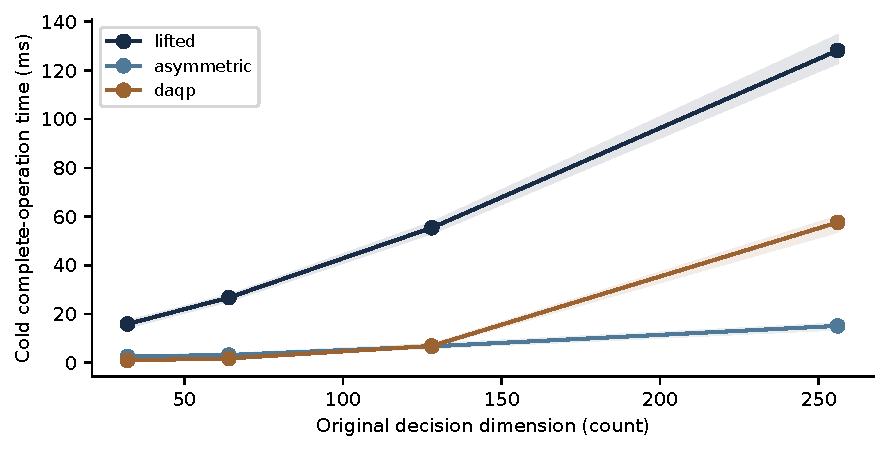
\includegraphics[width=.94\textwidth]{figures/cold-times.pdf}
\caption{Stored held-out asymmetric-elastic timing cells at density 0.05 and unit diagonal condition. Lines are stored medians and bands stored interquartile ranges; this descriptive subset does not replace the complete primary endpoint.}\label{fig:cold-times}
\end{figure}


The controlled conditioning results in Figure~\ref{fig:conditioning} retain
maximum objective discrepancy for each compatible robustness cell. The
finite grid extends to diagonal condition$10^6$, and its accepted observations
remain within the original objective and hard-row limits. The plot does not
establish stability for arbitrary nearly dependent rows, every semidefinite
problem, or an untested physical scaling. A missing method remains absent,
not an invented zero-error point. Relative objective agreement also does
not prove an identical dual vector when the mathematical dual is nonunique.
\begin{figure}[htbp]\centering
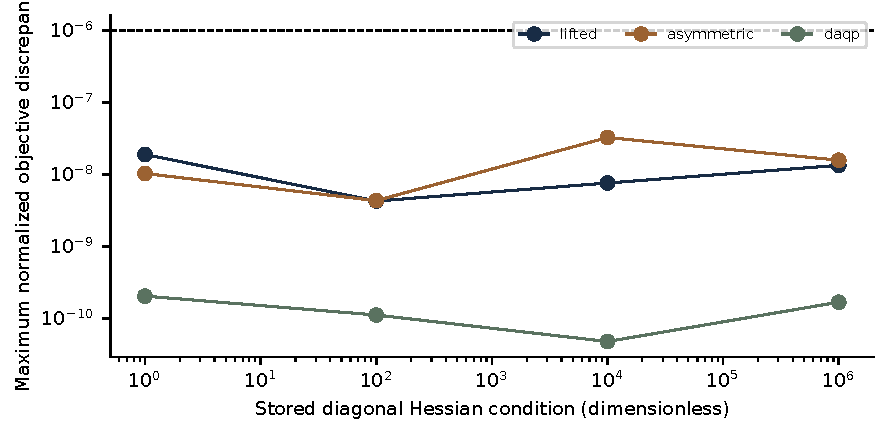
\includegraphics[width=.94\textwidth]{figures/conditioning.pdf}
\caption{Maximum stored objective discrepancy in each compatible robustness cell by diagonal condition. The dashed line is the original external objective criterion; absent methods remain absent rather than receiving an invented zero discrepancy.}\label{fig:conditioning}
\end{figure}


The common trajectory in Figure~\ref{fig:control-stream} shows the actual
stored position, velocity and bounded applied acceleration. It is driven
once by the independent oracle. Figure~\ref{fig:stream-reuse} compares stored
cold and warm operation durations along those same inputs. Workspace reuse
can reduce preparation work, but the stream alone cannot attribute every
timing difference solely to an active set, initial iterate or cached factor.
The plotted box summaries describe the retained observations; they are not
a new cluster-bootstrap experiment. Overlapping predicted horizon costs
remain distinct from realized plant cost.
\begin{figure}[htbp]\centering
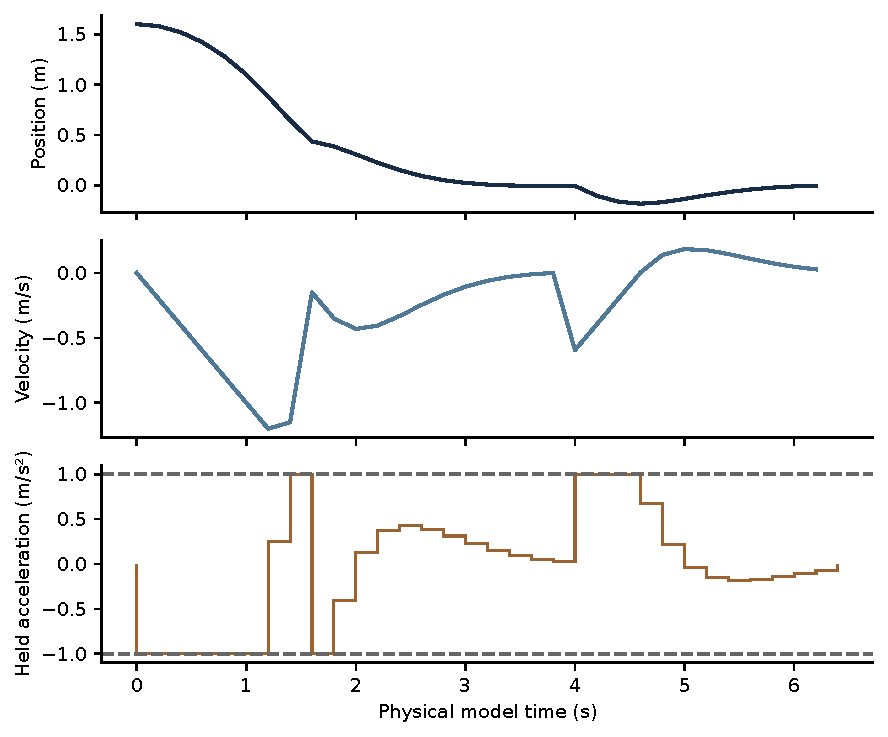
\includegraphics[width=.94\textwidth]{figures/control-stream.pdf}
\caption{The stored common C12 plant trajectory and interval-held oracle acceleration across thirty-two frames. Steps retain each complete physical sampling interval; these curves are not separate closed-loop controller performance measurements.}\label{fig:control-stream}
\end{figure}

\begin{figure}[htbp]\centering
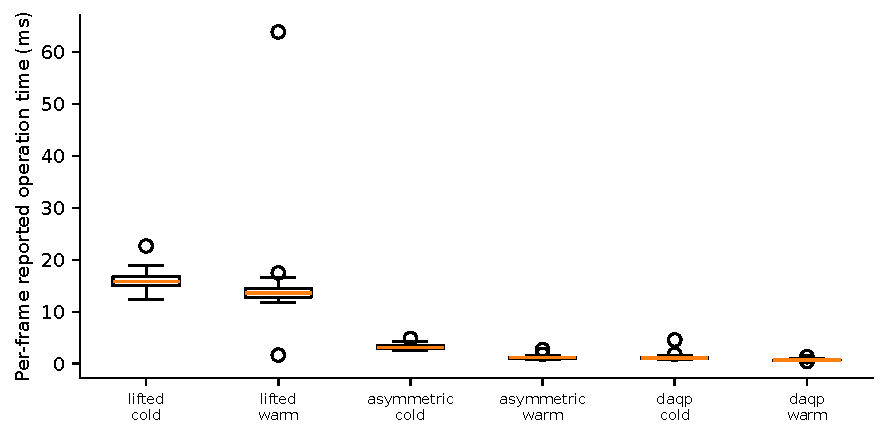
\includegraphics[width=.94\textwidth]{figures/stream-reuse.pdf}
\caption{Stored cold and warm C12 operation durations for every accepted frame of each compatible method. The box summaries are descriptive paired-path evidence, not a randomized causal isolation of warm starting from all other implementation choices.}\label{fig:stream-reuse}
\end{figure}


The grouped computation retains all 210 inputs. Table~\ref{tab:coupled-states}
and Figure~\ref{fig:coupled-states} account for all 5670 measured method
observations:3667 accepted,12 accuracy-rejected,1719 incompatible,270 dependent
oracle-failed and two timeouts. The larger raw inventory additionally retains
warm-ups and oracle observations. All 163390 returned candidate frames pass
their applicable original-space checks;44 noncandidate backend-limit frames
remain distinct. Those frame checks do not turn an iteration-limited batch
into an accepted primary operation.

The accuracy-rejected category must not be read as twelve returned
vectors violating the independent KKT calculation. The retained batches
include backend/iteration-limit or absent-vector outcomes; in particular,
six held-out row-split batches returned status seven without a candidate
vector. The two timeouts occurred in native and forced-proximal DAQP
operations. Six robustness oracle limits account for the dependent
144 measured oracle-failed rows in that split. These are operation and
dependency states, not additional independent KKT violations. Every
returned candidate frame still passed the applicable original-space checks.
\begin{table}[htbp]\centering\footnotesize
\caption{Measured grouped-study method states by split, including dependent oracle failures and supervised timeouts. Counts cover all measured method rows, while warm-up and oracle observations remain in the larger raw archive.}\label{tab:coupled-states}
\begin{tabularx}{\textwidth}{@{}>{\raggedright\arraybackslash}Xrrrrr@{}}\toprule
Split & Accepted & Accuracy & Incompat. & Oracle & Timeout\\\midrule
development & 879 & 0 & 396 & 21 & 0\\
heldout & 2587 & 6 & 1188 & 105 & 2\\
robustness & 201 & 6 & 135 & 144 & 0\\
\bottomrule\end{tabularx}
\end{table}

\begin{figure}[htbp]\centering
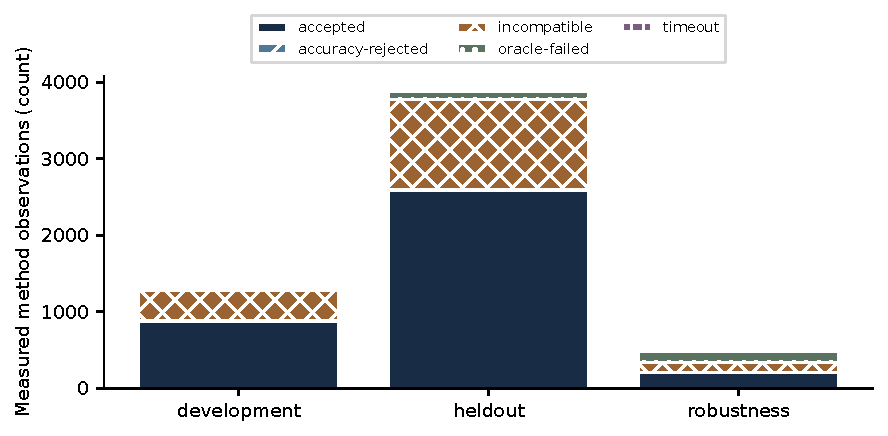
\includegraphics[width=.94\textwidth]{figures/coupled-states.pdf}
\caption{All 5670 measured method observations of the grouped study, separated by their original development, held-out and robustness splits. Acceptance, accuracy rejection, incompatibility, dependent oracle failure and supervised timeout remain different categories.}\label{fig:coupled-states}
\end{figure}


Figure~\ref{fig:coupled-population} retains all 144 primary members in their
stored order. Nine failed pairs keep their fixed score, and six missing
native medians remain gaps. No selected baseline is imputed where the
registered rule selected none. The primary median reduction is
\PrimaryEstimate\%, with 95\% limits \PrimaryLower\% and \PrimaryUpper\%.
These values do not define a uniform per-instance slowdown multiplier.
Figure~\ref{fig:coupled-formulations} displays returned method medians with
their unequal sample counts. It is a descriptive formulation comparison,
not an alternative matched estimator that removes failures or compatibility
differences. The original primary prediction is not rescued by those plots.
\begin{figure}[htbp]\centering
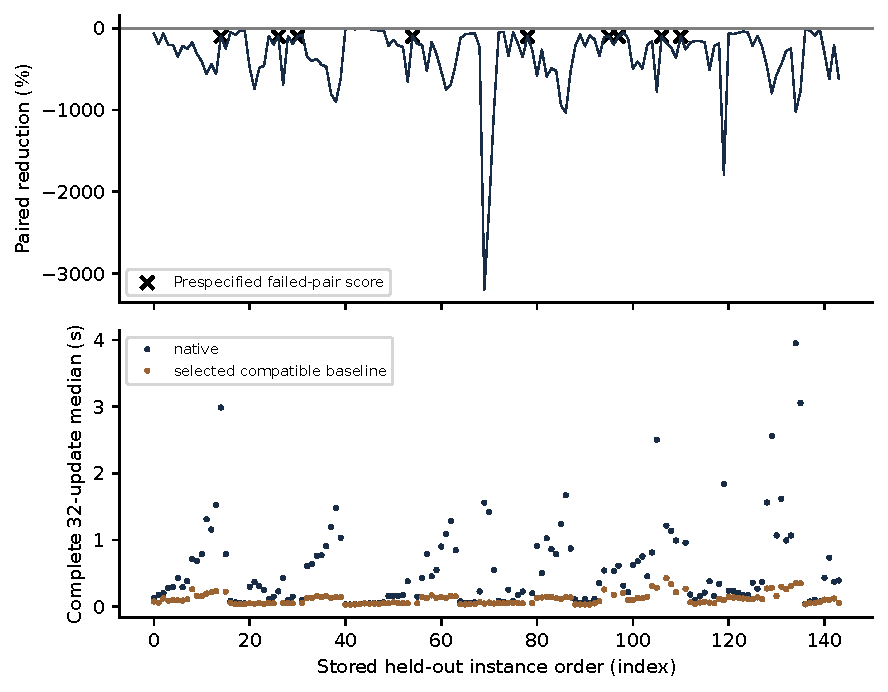
\includegraphics[width=.94\textwidth]{figures/coupled-population.pdf}
\caption{All 144 stored grouped-study primary members in original order, with nine failed scores retained. Complete-operation medians preserve missing values as gaps and do not impute a comparator where the primary rule selected none.}\label{fig:coupled-population}
\end{figure}

\begin{figure}[htbp]\centering
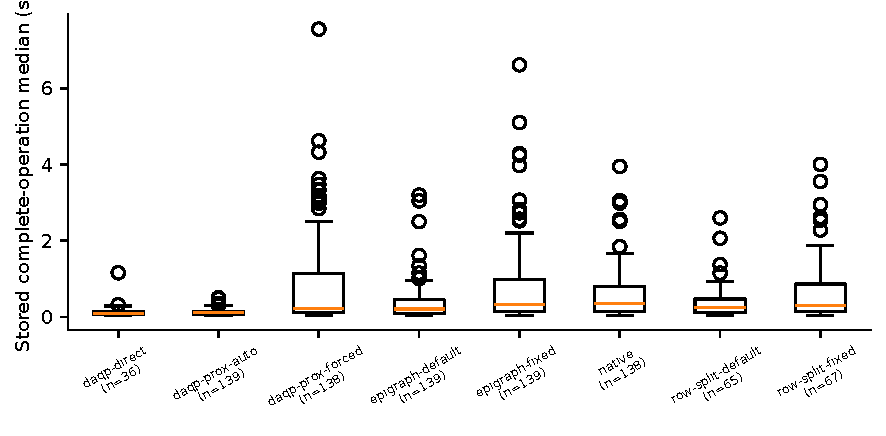
\includegraphics[width=.94\textwidth]{figures/coupled-formulations.pdf}
\caption{Distributions of stored held-out per-instance medians for each returned compatible formulation. Sample counts differ because compatibility and failures differ; these unmatched descriptive distributions are not the registered paired comparison or a causal ablation.}\label{fig:coupled-formulations}
\end{figure}


Finally, Figure~\ref{fig:directional-lesson} gives the stored native, epigraph
and directional row-split answers for the same two-variable physical teaching
input. Their objective and decision agreement illustrates representation
equivalence on a transparent example. It contributes no new timing sample
to either registered study. The dimensional covariance checks and policy
scale changes described in the teaching material distinguish preserving
physical meaning from intentionally changing a directional preference.
The coexistence of that numerical agreement with the complete negative
timing endpoint is the principal practical result: mathematical equivalence
and smaller principal dimensions do not guarantee a cheaper complete operation.
\begin{figure}[htbp]\centering
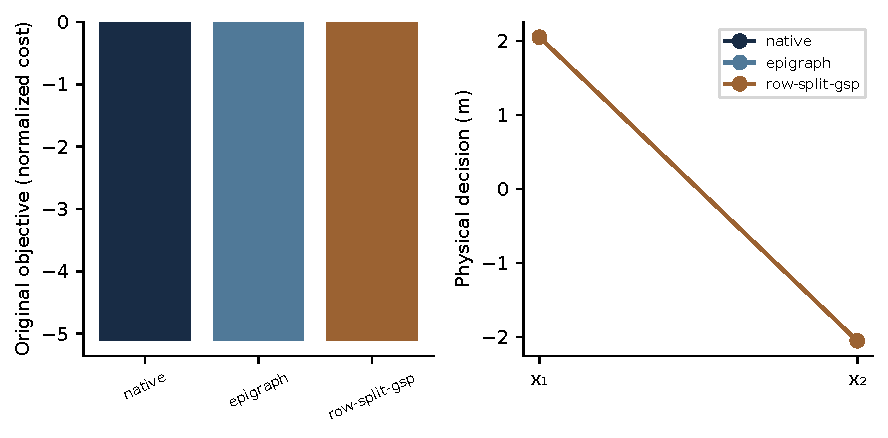
\includegraphics[width=.94\textwidth]{figures/directional-lesson.pdf}
\caption{Stored native, epigraph and directional row-split answers for the same two-variable physical teaching input. Objective and decision agreement are a small numerical illustration, not additional timing evidence or an independent experiment.}\label{fig:directional-lesson}
\end{figure}


\section{Validation}\label{sec:validation}
Validation starts in original coordinates. For a returned decision $x$, the
evaluator computes $Ax$, both departure arrays, the original base objective
and the exact requested penalty. Hard rows are tested without borrowing
the backend's internally scaled residual. The original timing criterion uses
\begin{equation}\label{eq:objective-discrepancy}
 \delta_F=\frac{|F(x)-F(x_\star)|}{\max\{1,|F(x_\star)|\}},\qquad
 h(x)=\max_{i\in\mathcal H}\max\{(\ell_i-A_ix)_+,(A_ix-u_i)_+\}.
\end{equation}
The independent lifted value $x_\star$ uses the matching objective, not a
solution of a symmetric or regularized surrogate. Both quantities must
satisfy their registered limits. The denominator in $\delta_F$ is a numerical
normalization, not a claim that objective scales from unrelated physical
models are interchangeable.
If the hard-row set is empty, its aggregate violation is defined as $h(x)=0$.
This global acceptance convention is distinct from a reader's unit-filtered
display, where no hard rows in the selected unit means that field is unavailable.

Primal--dual conditions add information beyond objective agreement. With
original multiplier $y$, stationarity and the soft subgradient condition are
\begin{equation}\label{eq:stationarity}
 Px+q+A^\top y=0,\qquad y\in\partial g(Ax).
\end{equation}
For separable costs, a proximal fixed-point check evaluates the second relation
without choosing an arbitrary derivative at a kink. The grouped study uses
the interval support and joint directional conjugate. For one group define
\begin{equation}\label{eq:group-dual-size}
 L_g(y)=\sum_{i\in I_g}\left(\frac{(y_i)_+}{c_{U,i}}+
                                  \frac{(-y_i)_+}{c_{L,i}}\right).
\end{equation}
Its residual-penalty conjugate is
\begin{equation}\label{eq:group-conjugate}
 \Psi_g^*(y)=\begin{cases}
 (L_g(y)-a_g)_+^2/(2b_g),&b_g>0,\\
 0,&b_g=0,\ L_g(y)\leq a_g,\\
 +\infty,&b_g=0,\ L_g(y)>a_g.
 \end{cases}
\end{equation}
The complete interval conjugate also contains the box support. Thus the
grouped dual condition is a joint price budget, not independent per-coordinate
caps. Every soft group's absolute normalized Fenchel gap and every hard
row's complementarity are checked separately. A signed aggregate gap is
retained diagnostically and cannot permit cross-row cancellation.

Raw and repaired dual quantities are distinguished. A bounded repair can
project small numerical defects onto an admissible dual domain, but its size
and effect on stationarity remain visible. An arbitrarily large repair would
erase the evidence that the returned dual was wrong. Candidate vectors are
checked frame by frame; backend-limit observations without vectors remain
noncandidates rather than acquiring synthetic coordinates. The 163390 returned
candidate frames and 44 noncandidate limit frames consequently have different
roles in the grouped validation record.

Physical covariance tests transform rows, bounds, prices, directions and
duals consistently. They exercise metre-to-centimetre and second-to-millisecond
maps in the predictive-control model and reciprocal directional row scaling
in the grouped teaching example. Negative controls omit or mismatch units,
change hard policy, reverse side signs and alter imported objectives. These
checks establish concrete semantic invariants; they do not prove every
floating-point computation invariant under arbitrary scaling. General
floating-point error and equilibration considerations remain relevant
background~\cite{higham,knight}.

The data boundaries have separate producer and consumer tests, including
fixture substitution, malformed arrays, unknown fields, cross-field mismatch,
stale source identity and rehashed tampering. Exact artifact hashes prove
identity only relative to a trusted inventory. They do not by themselves
prove numerical correctness, so source-bound independent acceptance is
retained separately. The same principle applies to a notebook execution
or a web screenshot: successful execution/rendering does not substitute
for inspecting what the method solved.

Additional solver literature informs the numerical reference choices without
becoming unexecuted performance evidence. Interior-point linear programming
and conic/QP implementations illustrate alternative handling of structure
and regularization~\cite{vanderbei,piqp}; those citations are not extra timed
competitors in the registered populations. Reproducible test infrastructure
and benchmark definitions are useful for future experiments~\cite{cutest},
but the present conclusions remain restricted to the exact synthetic inputs,
adapters, tolerances and complete operations actually recorded here.

\section{Discussion}\label{sec:discussion}
The two negative timing outcomes are consistent with the distinction between
algebraic size and numerical work. An original-row formulation can save
auxiliaries while adding a more expensive proximal operation, a threshold
sort, a source conversion or an acceptance calculation. Sparse factorization
also depends on fill, ordering, numeric scaling and reuse. Variable counts
alone do not measure these effects. The small C01 formulation comparison
therefore explains representation but cannot establish why a complete
repeated-forecast operation is faster or slower.

The strongest practical comparison is an equivalent objective with a capable
reference used according to its documented interface. Directional row
splitting is especially important because it reuses a published grouped
projection method to express unequal directions. Compact epigraphs offer
another exact route. Removing those references would test a weaker question.
Likewise, allowing only the candidate to preserve its workspace would build
an artificial advantage into repeated execution. Online active-set methods
have long exploited parametric structure~\cite{qpOASES}; a reuse mechanism
is not in itself evidence of a new algorithmic contribution.

The grouped threshold calculation has clear mathematical value even when
its runtime prediction fails. It exposes the actual directional metric,
zero-price behavior and joint dual budget. Those details make a correctness
check possible and clarify why a dense metric or overlapping groups require
additional analysis. Existing weighted projection algorithms and simplex/
norm-ball work provide relevant algorithmic background~\cite{weighted,duchi,condat}.
The implemented threshold is not presented as the first use of sorting,
orthant behavior or scalar active-prefix equations.

Numerical policy and physical policy must also remain distinct. A stronger
temperature price can reduce a comfort departure by changing the optimized
tradeoff, not by improving numerical accuracy. An oracle-driven predictive
trajectory can isolate solver agreement on common inputs, not demonstrate
that separately optimized controllers have equal field behavior. For energy
examples, comparing a mixed group/Huber optimum with an authored separable
variant describes a policy change. These distinctions limit what a
practitioner should infer from cross-case objective tables and interactive
cost edits.

The results suggest choosing an admitted exact formulation based on the
actual problem regime and measured complete-operation requirements, rather
than adopting the smallest principal matrix by default. Where hard policy
is immutable, a method that cannot preserve it should be refused. Where
uncertainty about physical coefficients dominates numerical error, tighter
solver tolerances do not certify a better operational model. A future
computational prediction should specify a new mechanism and evaluation
prospectively; the existing held-out data cannot be retuned into evidence
for a revised threshold, population or favorable subset.

The system's inspectability remains useful despite the failed performance
criteria. Original-space quantities, exact compatibility and retained
unsuccessful outcomes let a reader distinguish an implementation defect
from an objective mismatch or a negative computational finding. They do
not establish adoption, realized savings or safety. Those questions require
different data, deployment conditions and evidence than the synthetic
optimization studies described here.

\section{Limitations}\label{sec:limitations}
The inputs are transparent synthetic optimization models. The source-faithful
building example preserves an open model rather than observations from an
occupied building. Its battery and thermal parameters are not identified
from a particular installation. The grouped thermal study uses a separate
hourly RC forecast model. Neither model supports a claim about actual
energy savings, occupant comfort, component ageing or operational safety.
Those outcomes require measured disturbances, identification uncertainty,
actuator behavior and a separately validated control policy.

The timing studies were executed on one nonreserved host with explicit
software identities and resource boundaries. Fixed seeds and randomized
method order improve reproducibility but do not eliminate operating-system
interference, thermal throttling, library maturity or language-level
overhead. The Python/SciPy FlexQP reconstruction and native C backends
are concrete implementations with different engineering histories. Their
runtime difference is not a formulation-independent theorem. Backend setup
includes linear-system preparation; isolated numeric factor time was not
instrumented and cannot be inferred from a setup field.

Statistical generalization is limited by the prospective populations and
few seed clusters. Original repeated observations are dependent within
generated problems and seeds. The cluster procedure respects a selected
dependence structure, but six clusters do not guarantee accurate coverage
under every disturbance or sampling process~\cite{cameron}. The grouped
score includes the prescribed failed-pair treatment. Its negative median
is not a universal latency multiplier. Unmatched method distributions and
selected descriptive slices cannot replace either registered paired endpoint.

The mathematical scope is also explicit. The group proximal identity uses
nonempty closed boxes, contraction-monotone convex prices and a fixed
positive diagonal metric. The native grouped interface requires disjoint
groups and positive finite directional scales. The convergence statement
assumes an attained saddle point and the specified relaxation range; it
does not establish arbitrary adaptive metrics, overlapping groups,
nonconvex curvature or every finite-precision infeasibility certificate.
The synthetic robustness grid is finite, so passing it does not certify
all nearly singular or physically scaled problems.

Finally, the browser verifies and presents existing results and matching
local-native imports. It has no browser-native optimizer or hosted
optimization service, and the grouped research exchanges have no installed
replay adapter. A published package, a schema example and a successful
render are different kinds of availability evidence. Deep FlexQP's trained
policy was unavailable and is not reproduced. The complete negative
findings remain scientifically informative within these restrictions,
without establishing algorithmic priority, superiority, practical adoption
or a qualified production control system.

\section{Reproducibility}\label{sec:reproducibility}
The public source repository is
\url{https://github.com/fsantibanezleal/CAOS_SoftQP}; the separate native engine
is \url{https://github.com/fsantibanezleal/CAOS_SoftQP_Engine}.
The original study uses its recorded native source identity, which must not
be equated silently with a later public wheel. The grouped study uses the
separate pinned SDK 0.2 profile and registered protocol/source map. Replaying
archived observations does not require rerunning timing measurements.

The grouped evidence dataset is available at
\url{https://doi.org/10.5281/zenodo.23875194}. The stored original summaries % voice-ok: cited supporting dataset identity, not this document's deposit narrative
and common control trajectory are \path{data/derived/experiments/campaign.json} % voice-ok: literal public evidence filename
and \path{data/derived/experiments/stream.json} in the product source at
\url{https://github.com/fsantibanezleal/CAOS_SoftQP/tree/2d3f299d80edad49c2599e61bb6e3c875c119043}.
The original computation used native engine source
\path{d0c69ed974d577ba02adbd4806332270d9425651}; the grouped registered
implementation used source \path{246bf87e690f4d010494c556e2021d311d587422}.
The grouped archive contains the protocol and complete observations; its
summary is also \path{manuscripts/coupled-peak-study/results/summary/summary.json}
in that frozen product tree. These identifiers locate the numerical evidence
independently of later manuscript presentation changes.

The committed manuscript asset generator reads immutable scientific inputs,
checks their Git identities and emits vector PDF figures, literal result
tables and source manifests. Running
\texttt{python manuscripts/shared/generate\_assets.py} rebuilds those assets
without solving a model or recomputing a confidence interval. Each document's
\texttt{build.py} verifies numeric sources and compiles native LaTeX with
BibTeX, refusing unresolved or clipped output. The manuscript rendering
requirements are pinned separately from numerical experiment environments.

The full grouped data include canonical batches, complete JSONL/CSV,
protocol snapshots, environment identities, unsuccessful observations and
replay validation. Reproduction of a new timing study requires an exact
historical source/environment checkout and a new external output directory;
such a rerun is not needed to inspect the preserved results. Large study
outputs, temporary files and scientific environments use external role
roots. No secret token or private operational dataset is required to read
the scientific inputs or reconstruct the published figures and tables.

\paragraph{Declaration of generative AI use.}
Generative AI tools assisted source synthesis, mathematical checking,
implementation and drafting. Numerical and editorial claims were checked
against independent formulations and preserved computational evidence.
Responsibility for the work rests with the named author.

\section{Conclusions}\label{sec:conclusions}
An explicit hard/soft policy, original-space objective and versioned exchange
boundaries make a convex optimization result inspectable. The implemented
system compares seven method paths across their actual compatibility
domains, preserves physical row units and supports native execution,
independent evaluation, verified replay and matching local result import.
Equivalent lifting and directional reformulations show that representation
choices must be assessed on the same objective rather than on similarly
named soft constraints.

The complete original 456-instance study does not establish its 10\% timing
prediction: the stored median reduction is \OriginalEstimate\%, with a 95\%
interval from \OriginalLower\% to \OriginalUpper\%. The separate grouped
study likewise does not establish improvement: its 144-instance primary
score is \PrimaryEstimate\%, with limits \PrimaryLower\% and \PrimaryUpper\%
and \PrimaryFailed{} retained failed pairs. These are separate inferential
results with different measurement scopes, not interchangeable runtime
rankings or a uniform slowdown statement.

Original-row proximal calculations can be mathematically exact and still
fail to reduce complete-operation cost. Future work should identify a
specific mechanism, preserve the strongest compatible references and
evaluate a prospective population. The current synthetic evidence supports
reproducible modeling and numerical investigation; it does not establish
field benefit, safety or algorithmic priority.

\appendix

\section{Complete nested contract fields}\label{sec:contract-appendix}

The following schema-derived tables expand nested sparse matrices, original row
metadata, method outputs, update vectors and numerical diagnostics. Their field
paths retain array markers and alternative branches so an object-level summary
cannot hide the type or bound of a numerical child. Structural restrictions are
copied literally from the identified schema. Paths marked if identify a predicate;
then and else specify its respective consequences. A not branch forbids its
displayed condition; contains with minContains specifies required matching
array members. These branch markers preserve conditional meaning rather than
asserting every alternative simultaneously. Physical dimensions are interpreted
through the original model and its explicit unit maps; a metadata container has
no single physical unit merely because it contains numerical values.

The schemas establish structural admission rather than convexity, physical
adequacy or scientific optimality. Cross-field requirements described in the
data section still apply: sparse pointer consistency, matching vector lengths,
unchanged hard policy, exact request identity, group membership and complete
experimental populations cannot be inferred by counting table rows. Likewise,
a unit symbol is not a numerical conversion and an absent result is not zero.
This appendix complements the numerical derivations and producer/consumer
descriptions; it does not replace original-space evaluation. Each table names
the exact contract whose complete fields it expands, keeping the parameter
meaning inspectable without treating a schema example as available browser
data or a proof of successful solver execution.

Nested fields of case-index are enumerated in Table~\ref{tab:nested-case-index}.

\begingroup\footnotesize\setlength{\tabcolsep}{3pt}
\begin{longtable}{@{}>{\raggedright\arraybackslash}p{.25\textwidth}>{\raggedright\arraybackslash}p{.11\textwidth}>{\raggedright\arraybackslash}p{.37\textwidth}>{\raggedright\arraybackslash}p{.20\textwidth}@{}}
\caption{Complete nested fields, value types, literal schema restrictions and physical or structural dimensions for case-index. Required and optional structures retain the original schema and model interpretation.}\label{tab:nested-case-index}\\
\toprule Field path & Type & Restrictions & Unit / role\\\midrule\endfirsthead
\toprule Field path & Type & Restrictions & Unit / role\\\midrule\endhead
\bottomrule\endfoot
schema & string & const=\allowbreak{}softqp.\allowbreak{}artifact-\allowbreak{}index/\allowbreak{}v1 & structural metadata /\allowbreak{} nested units\\
engine\_\allowbreak{}version & string & See defined object /\allowbreak{} value type & structural metadata /\allowbreak{} nested units\\
n\_\allowbreak{}cases & integer & minimum=\allowbreak{}1 & count /\allowbreak{} integer identifier\\
default\_\allowbreak{}case & string & pattern=\allowbreak{}\textasciicircum{}C[0-9]\{2\}\$ & structural metadata /\allowbreak{} nested units\\
cases & array & minItems=\allowbreak{}1 & structural metadata /\allowbreak{} nested units\\
cases[] & object & additionalProperties=\allowbreak{}False; required=\allowbreak{}['case\_\allowbreak{}id', 'title', 'category', 'manifest\_\allowbreak{}path'] & structural metadata /\allowbreak{} nested units\\
cases[].\allowbreak{}case\_\allowbreak{}id & string & pattern=\allowbreak{}\textasciicircum{}C[0-9]\{2\}\$ & structural metadata /\allowbreak{} nested units\\
cases[].\allowbreak{}title & object & additionalProperties=\allowbreak{}False; required=\allowbreak{}['en', 'es'] & structural metadata /\allowbreak{} nested units\\
cases[].\allowbreak{}title.\allowbreak{}en & string & minLength=\allowbreak{}1 & structural metadata /\allowbreak{} nested units\\
cases[].\allowbreak{}title.\allowbreak{}es & string & minLength=\allowbreak{}1 & structural metadata /\allowbreak{} nested units\\
cases[].\allowbreak{}category & object & additionalProperties=\allowbreak{}False; required=\allowbreak{}['en', 'es'] & structural metadata /\allowbreak{} nested units\\
cases[].\allowbreak{}category.\allowbreak{}en & string & minLength=\allowbreak{}1 & structural metadata /\allowbreak{} nested units\\
cases[].\allowbreak{}category.\allowbreak{}es & string & minLength=\allowbreak{}1 & structural metadata /\allowbreak{} nested units\\
cases[].\allowbreak{}manifest\_\allowbreak{}path & string & pattern=\allowbreak{}\textasciicircum{}(?!.\allowbreak{}*\textbackslash{}.\allowbreak{}\textbackslash{}.\allowbreak{})[A-\allowbreak{}Za-\allowbreak{}z0-9\_\allowbreak{}.\allowbreak{}/\allowbreak{}-]+\textbackslash{}.\allowbreak{}json\$ & structural metadata /\allowbreak{} nested units\\
files & array & uniqueItems=\allowbreak{}True & structural metadata /\allowbreak{} nested units\\
files[] & string & pattern=\allowbreak{}\textasciicircum{}(?!.\allowbreak{}*\textbackslash{}.\allowbreak{}\textbackslash{}.\allowbreak{})[A-\allowbreak{}Za-\allowbreak{}z0-9\_\allowbreak{}.\allowbreak{}/\allowbreak{}-]+\textbackslash{}.\allowbreak{}(json\textbar{}\allowbreak{}csv\textbar{}\allowbreak{}jsonl)\$ & structural metadata /\allowbreak{} nested units\\
\end{longtable}\endgroup


Nested fields of case-manifest are enumerated in Table~\ref{tab:nested-case-manifest}.

\begingroup\footnotesize\setlength{\tabcolsep}{3pt}
\begin{longtable}{@{}>{\raggedright\arraybackslash}p{.25\textwidth}>{\raggedright\arraybackslash}p{.11\textwidth}>{\raggedright\arraybackslash}p{.37\textwidth}>{\raggedright\arraybackslash}p{.20\textwidth}@{}}
\caption{Complete nested fields, value types, literal schema restrictions and physical or structural dimensions for case-manifest. Required and optional structures retain the original schema and model interpretation.}\label{tab:nested-case-manifest}\\
\toprule Field path & Type & Restrictions & Unit / role\\\midrule\endfirsthead
\toprule Field path & Type & Restrictions & Unit / role\\\midrule\endhead
\bottomrule\endfoot
schema & string & const=\allowbreak{}softqp.\allowbreak{}manifest/\allowbreak{}v1 & structural metadata /\allowbreak{} nested units\\
case\_\allowbreak{}id & string & pattern=\allowbreak{}\textasciicircum{}C[0-9]\{2\}\$ & structural metadata /\allowbreak{} nested units\\
title & object & additionalProperties=\allowbreak{}False; required=\allowbreak{}['en', 'es'] & structural metadata /\allowbreak{} nested units\\
title.\allowbreak{}en & string & minLength=\allowbreak{}1 & structural metadata /\allowbreak{} nested units\\
title.\allowbreak{}es & string & minLength=\allowbreak{}1 & structural metadata /\allowbreak{} nested units\\
category & object & additionalProperties=\allowbreak{}False; required=\allowbreak{}['en', 'es'] & structural metadata /\allowbreak{} nested units\\
category.\allowbreak{}en & string & minLength=\allowbreak{}1 & structural metadata /\allowbreak{} nested units\\
category.\allowbreak{}es & string & minLength=\allowbreak{}1 & structural metadata /\allowbreak{} nested units\\
engine & object & additionalProperties=\allowbreak{}False; required=\allowbreak{}['package', 'version'] & structural metadata /\allowbreak{} nested units\\
engine.\allowbreak{}package & string & const=\allowbreak{}softqp & structural metadata /\allowbreak{} nested units\\
engine.\allowbreak{}version & string & See defined object /\allowbreak{} value type & structural metadata /\allowbreak{} nested units\\
product\_\allowbreak{}version & string & See defined object /\allowbreak{} value type & structural metadata /\allowbreak{} nested units\\
seed & integer & See defined object /\allowbreak{} value type & count /\allowbreak{} integer identifier\\
source & string & See defined object /\allowbreak{} value type & structural metadata /\allowbreak{} nested units\\
artifact & object & additionalProperties=\allowbreak{}False; required=\allowbreak{}['path', 'bytes', 'sha256', 'format'] & structural metadata /\allowbreak{} nested units\\
artifact.\allowbreak{}path & string & pattern=\allowbreak{}\textasciicircum{}(?!.\allowbreak{}*\textbackslash{}.\allowbreak{}\textbackslash{}.\allowbreak{})[A-\allowbreak{}Za-\allowbreak{}z0-9\_\allowbreak{}.\allowbreak{}/\allowbreak{}-]+\textbackslash{}.\allowbreak{}json\$ & structural metadata /\allowbreak{} nested units\\
artifact.\allowbreak{}bytes & integer & minimum=\allowbreak{}1 & bytes\\
artifact.\allowbreak{}sha256 & string & pattern=\allowbreak{}\textasciicircum{}[0-9a-\allowbreak{}f]\{64\}\$ & structural metadata /\allowbreak{} nested units\\
artifact.\allowbreak{}format & string & const=\allowbreak{}json & structural metadata /\allowbreak{} nested units\\
lane & string & const=\allowbreak{}precompute & structural metadata /\allowbreak{} nested units\\
gate & object & additionalProperties=\allowbreak{}False; required=\allowbreak{}['lane', 'reasons'] & structural metadata /\allowbreak{} nested units\\
gate.\allowbreak{}lane & string & const=\allowbreak{}precompute & structural metadata /\allowbreak{} nested units\\
gate.\allowbreak{}reasons & array & minItems=\allowbreak{}1 & structural metadata /\allowbreak{} nested units\\
gate.\allowbreak{}reasons[] & object & additionalProperties=\allowbreak{}False; required=\allowbreak{}['en', 'es'] & structural metadata /\allowbreak{} nested units\\
gate.\allowbreak{}reasons[].\allowbreak{}en & string & minLength=\allowbreak{}1 & structural metadata /\allowbreak{} nested units\\
gate.\allowbreak{}reasons[].\allowbreak{}es & string & minLength=\allowbreak{}1 & structural metadata /\allowbreak{} nested units\\
\end{longtable}\endgroup


Nested fields of readiness are enumerated in Table~\ref{tab:nested-readiness}.

\begingroup\footnotesize\setlength{\tabcolsep}{3pt}
\begin{longtable}{@{}>{\raggedright\arraybackslash}p{.25\textwidth}>{\raggedright\arraybackslash}p{.11\textwidth}>{\raggedright\arraybackslash}p{.37\textwidth}>{\raggedright\arraybackslash}p{.20\textwidth}@{}}
\caption{Complete nested fields, value types, literal schema restrictions and physical or structural dimensions for readiness. Required and optional structures retain the original schema and model interpretation.}\label{tab:nested-readiness}\\
\toprule Field path & Type & Restrictions & Unit / role\\\midrule\endfirsthead
\toprule Field path & Type & Restrictions & Unit / role\\\midrule\endhead
\bottomrule\endfoot
schema & string & const=\allowbreak{}softqp.\allowbreak{}readiness/\allowbreak{}v2 & structural metadata /\allowbreak{} nested units\\
product\_\allowbreak{}version & string & pattern=\allowbreak{}\textasciicircum{}\textbackslash{}d+\textbackslash{}.\allowbreak{}\textbackslash{}d\{2\}\textbackslash{}.\allowbreak{}\textbackslash{}d\{3\}\$ & structural metadata /\allowbreak{} nested units\\
catalog\_\allowbreak{}sha256 & string & pattern=\allowbreak{}\textasciicircum{}[0-9a-\allowbreak{}f]\{64\}\$ & structural metadata /\allowbreak{} nested units\\
contracts & array & minItems=\allowbreak{}1 & structural metadata /\allowbreak{} nested units\\
contracts[] & object & additionalProperties=\allowbreak{}False; required=\allowbreak{}['id', 'version', 'status', 'provenance', 'state', 'reason', 'missing'] & structural metadata /\allowbreak{} nested units\\
contracts[].\allowbreak{}id & string & pattern=\allowbreak{}\textasciicircum{}[a-\allowbreak{}z0-9][a-\allowbreak{}z0-9-]*\$ & structural metadata /\allowbreak{} nested units\\
contracts[].\allowbreak{}version & string & pattern=\allowbreak{}\textasciicircum{}\textbackslash{}d+\textbackslash{}.\allowbreak{}\textbackslash{}d+\textbackslash{}.\allowbreak{}\textbackslash{}d+\$ & structural metadata /\allowbreak{} nested units\\
contracts[].\allowbreak{}status & enumerated value & enum=\allowbreak{}['real', 'active'] & structural metadata /\allowbreak{} nested units\\
contracts[].\allowbreak{}provenance & enumerated value & enum=\allowbreak{}['real', 'stub', 'simulator', 'fixture', 'baseline', None] & structural metadata /\allowbreak{} nested units\\
contracts[].\allowbreak{}state & enumerated value & enum=\allowbreak{}['available', 'partial', 'stale', 'provider', 'training', 'missing'] & structural metadata /\allowbreak{} nested units\\
contracts[].\allowbreak{}reason & union /\allowbreak{} composition & See defined object /\allowbreak{} value type & structural metadata /\allowbreak{} nested units\\
contracts[].\allowbreak{}reason (oneOf1) & object & additionalProperties=\allowbreak{}False; required=\allowbreak{}['en', 'es'] & structural metadata /\allowbreak{} nested units\\
contracts[].\allowbreak{}reason (oneOf1).\allowbreak{}en & string & minLength=\allowbreak{}1 & structural metadata /\allowbreak{} nested units\\
contracts[].\allowbreak{}reason (oneOf1).\allowbreak{}es & string & minLength=\allowbreak{}1 & structural metadata /\allowbreak{} nested units\\
contracts[].\allowbreak{}reason (oneOf2) & null & See defined object /\allowbreak{} value type & structural metadata /\allowbreak{} nested units\\
contracts[].\allowbreak{}missing & array & See defined object /\allowbreak{} value type & structural metadata /\allowbreak{} nested units\\
contracts[].\allowbreak{}missing[] & string & See defined object /\allowbreak{} value type & structural metadata /\allowbreak{} nested units\\
contracts[] (allOf1) & object & See defined object /\allowbreak{} value type & structural metadata /\allowbreak{} nested units\\
contracts[] (allOf1) (if) & object & See defined object /\allowbreak{} value type & structural metadata /\allowbreak{} nested units\\
contracts[] (allOf1) (if).\allowbreak{}state & string & const=\allowbreak{}available & structural metadata /\allowbreak{} nested units\\
contracts[] (allOf1) (then) & object & See defined object /\allowbreak{} value type & structural metadata /\allowbreak{} nested units\\
contracts[] (allOf1) (then).\allowbreak{}reason & null & See defined object /\allowbreak{} value type & structural metadata /\allowbreak{} nested units\\
contracts[] (allOf1) (then).\allowbreak{}provenance & string & const=\allowbreak{}real & structural metadata /\allowbreak{} nested units\\
contracts[] (allOf1) (else) & object & See defined object /\allowbreak{} value type & structural metadata /\allowbreak{} nested units\\
contracts[] (allOf1) (else).\allowbreak{}reason & object & additionalProperties=\allowbreak{}False; required=\allowbreak{}['en', 'es'] & structural metadata /\allowbreak{} nested units\\
contracts[] (allOf1) (else).\allowbreak{}reason.\allowbreak{}en & string & minLength=\allowbreak{}1 & structural metadata /\allowbreak{} nested units\\
contracts[] (allOf1) (else).\allowbreak{}reason.\allowbreak{}es & string & minLength=\allowbreak{}1 & structural metadata /\allowbreak{} nested units\\
contracts[] (allOf2) & object & See defined object /\allowbreak{} value type & structural metadata /\allowbreak{} nested units\\
contracts[] (allOf2) (if) & object & See defined object /\allowbreak{} value type & structural metadata /\allowbreak{} nested units\\
contracts[] (allOf2) (if).\allowbreak{}state & string & const=\allowbreak{}partial & structural metadata /\allowbreak{} nested units\\
contracts[] (allOf2) (then) & object & See defined object /\allowbreak{} value type & structural metadata /\allowbreak{} nested units\\
contracts[] (allOf2) (then).\allowbreak{}missing & array & minItems=\allowbreak{}1 & structural metadata /\allowbreak{} nested units\\
contracts[] (allOf2) (else) & object & See defined object /\allowbreak{} value type & structural metadata /\allowbreak{} nested units\\
contracts[] (allOf2) (else).\allowbreak{}missing & array & maxItems=\allowbreak{}0 & structural metadata /\allowbreak{} nested units\\
contracts[] (allOf3) & object & See defined object /\allowbreak{} value type & structural metadata /\allowbreak{} nested units\\
contracts[] (allOf3) (if) & object & See defined object /\allowbreak{} value type & structural metadata /\allowbreak{} nested units\\
contracts[] (allOf3) (if).\allowbreak{}state & string & const=\allowbreak{}missing & structural metadata /\allowbreak{} nested units\\
contracts[] (allOf3) (then) & object & See defined object /\allowbreak{} value type & structural metadata /\allowbreak{} nested units\\
contracts[] (allOf3) (then).\allowbreak{}provenance & null & See defined object /\allowbreak{} value type & structural metadata /\allowbreak{} nested units\\
contracts[] (allOf3) (else) & object & See defined object /\allowbreak{} value type & structural metadata /\allowbreak{} nested units\\
contracts[] (allOf3) (else).\allowbreak{}provenance & string & See defined object /\allowbreak{} value type & structural metadata /\allowbreak{} nested units\\
contracts[] (allOf4) & object & See defined object /\allowbreak{} value type & structural metadata /\allowbreak{} nested units\\
contracts[] (allOf4) (if) & object & See defined object /\allowbreak{} value type & structural metadata /\allowbreak{} nested units\\
contracts[] (allOf4) (if).\allowbreak{}state & string & const=\allowbreak{}provider & structural metadata /\allowbreak{} nested units\\
contracts[] (allOf4) (then) & object & See defined object /\allowbreak{} value type & structural metadata /\allowbreak{} nested units\\
contracts[] (allOf4) (then).\allowbreak{}provenance & enumerated value & enum=\allowbreak{}['stub', 'simulator', 'fixture', 'baseline'] & structural metadata /\allowbreak{} nested units\\
contracts[] (allOf5) & object & See defined object /\allowbreak{} value type & structural metadata /\allowbreak{} nested units\\
contracts[] (allOf5) (if) & object & See defined object /\allowbreak{} value type & structural metadata /\allowbreak{} nested units\\
contracts[] (allOf5) (if).\allowbreak{}state & string & const=\allowbreak{}training & structural metadata /\allowbreak{} nested units\\
contracts[] (allOf5) (then) & object & See defined object /\allowbreak{} value type & structural metadata /\allowbreak{} nested units\\
contracts[] (allOf5) (then).\allowbreak{}provenance & enumerated value & enum=\allowbreak{}['real', 'baseline'] & structural metadata /\allowbreak{} nested units\\
contracts[] (allOf6) & object & See defined object /\allowbreak{} value type & structural metadata /\allowbreak{} nested units\\
contracts[] (allOf6) (if) & object & See defined object /\allowbreak{} value type & structural metadata /\allowbreak{} nested units\\
contracts[] (allOf6) (if).\allowbreak{}status & string & const=\allowbreak{}active & structural metadata /\allowbreak{} nested units\\
contracts[] (allOf6) (then) & object & See defined object /\allowbreak{} value type & structural metadata /\allowbreak{} nested units\\
contracts[] (allOf6) (then).\allowbreak{}provenance & object & See defined object /\allowbreak{} value type & structural metadata /\allowbreak{} nested units\\
contracts[] (allOf6) (then).\allowbreak{}provenance (not) & string & const=\allowbreak{}real & structural metadata /\allowbreak{} nested units\\
\end{longtable}\endgroup


Nested fields of api are enumerated in Table~\ref{tab:nested-api}.

\begingroup\footnotesize\setlength{\tabcolsep}{3pt}
\begin{longtable}{@{}>{\raggedright\arraybackslash}p{.25\textwidth}>{\raggedright\arraybackslash}p{.11\textwidth}>{\raggedright\arraybackslash}p{.37\textwidth}>{\raggedright\arraybackslash}p{.20\textwidth}@{}}
\caption{Complete nested fields, value types, literal schema restrictions and physical or structural dimensions for api. Required and optional structures retain the original schema and model interpretation.}\label{tab:nested-api}\\
\toprule Field path & Type & Restrictions & Unit / role\\\midrule\endfirsthead
\toprule Field path & Type & Restrictions & Unit / role\\\midrule\endhead
\bottomrule\endfoot
detail & object & additionalProperties=\allowbreak{}False; required=\allowbreak{}['state', 'reason'] & structural metadata /\allowbreak{} nested units\\
detail.\allowbreak{}state & string & const=\allowbreak{}missing & structural metadata /\allowbreak{} nested units\\
detail.\allowbreak{}reason & object & additionalProperties=\allowbreak{}False; required=\allowbreak{}['en', 'es'] & structural metadata /\allowbreak{} nested units\\
detail.\allowbreak{}reason.\allowbreak{}en & string & minLength=\allowbreak{}1 & structural metadata /\allowbreak{} nested units\\
detail.\allowbreak{}reason.\allowbreak{}es & string & minLength=\allowbreak{}1 & structural metadata /\allowbreak{} nested units\\
\end{longtable}\endgroup


Nested fields of softqp-index are enumerated in Table~\ref{tab:nested-softqp-index}.

\begingroup\footnotesize\setlength{\tabcolsep}{3pt}
\begin{longtable}{@{}>{\raggedright\arraybackslash}p{.25\textwidth}>{\raggedright\arraybackslash}p{.11\textwidth}>{\raggedright\arraybackslash}p{.37\textwidth}>{\raggedright\arraybackslash}p{.20\textwidth}@{}}
\caption{Complete nested fields, value types, literal schema restrictions and physical or structural dimensions for softqp-index. Required and optional structures retain the original schema and model interpretation.}\label{tab:nested-softqp-index}\\
\toprule Field path & Type & Restrictions & Unit / role\\\midrule\endfirsthead
\toprule Field path & Type & Restrictions & Unit / role\\\midrule\endhead
\bottomrule\endfoot
schema\_\allowbreak{}version & string & const=\allowbreak{}softqp.\allowbreak{}index/\allowbreak{}v1 & structural metadata /\allowbreak{} nested units\\
state & string & const=\allowbreak{}development & structural metadata /\allowbreak{} nested units\\
default\_\allowbreak{}case & union /\allowbreak{} composition & See defined object /\allowbreak{} value type & structural metadata /\allowbreak{} nested units\\
default\_\allowbreak{}case (anyOf1) & string & pattern=\allowbreak{}\textasciicircum{}C[0-9]\{2\}\$ & structural metadata /\allowbreak{} nested units\\
default\_\allowbreak{}case (anyOf2) & null & See defined object /\allowbreak{} value type & structural metadata /\allowbreak{} nested units\\
cases & array & See defined object /\allowbreak{} value type & structural metadata /\allowbreak{} nested units\\
cases[] & object & additionalProperties=\allowbreak{}False; required=\allowbreak{}['case\_\allowbreak{}id', 'title', 'category', 'path', 'sha256', 'failed'] & structural metadata /\allowbreak{} nested units\\
cases[].\allowbreak{}case\_\allowbreak{}id & string & pattern=\allowbreak{}\textasciicircum{}C[0-9]\{2\}\$ & structural metadata /\allowbreak{} nested units\\
cases[].\allowbreak{}title & object & additionalProperties=\allowbreak{}False; required=\allowbreak{}['en', 'es'] & structural metadata /\allowbreak{} nested units\\
cases[].\allowbreak{}title.\allowbreak{}en & string & minLength=\allowbreak{}1 & structural metadata /\allowbreak{} nested units\\
cases[].\allowbreak{}title.\allowbreak{}es & string & minLength=\allowbreak{}1 & structural metadata /\allowbreak{} nested units\\
cases[].\allowbreak{}category & object & additionalProperties=\allowbreak{}False; required=\allowbreak{}['en', 'es'] & structural metadata /\allowbreak{} nested units\\
cases[].\allowbreak{}category.\allowbreak{}en & string & minLength=\allowbreak{}1 & structural metadata /\allowbreak{} nested units\\
cases[].\allowbreak{}category.\allowbreak{}es & string & minLength=\allowbreak{}1 & structural metadata /\allowbreak{} nested units\\
cases[].\allowbreak{}path & string & pattern=\allowbreak{}\textasciicircum{}C[0-9]\{2\}\textbackslash{}.\allowbreak{}json\$ & structural metadata /\allowbreak{} nested units\\
cases[].\allowbreak{}sha256 & string & pattern=\allowbreak{}\textasciicircum{}[a-\allowbreak{}f0-9]\{64\}\$ & structural metadata /\allowbreak{} nested units\\
cases[].\allowbreak{}failed & boolean & See defined object /\allowbreak{} value type & structural metadata /\allowbreak{} nested units\\
environment & object & additionalProperties=\allowbreak{}False; required=\allowbreak{}['python', 'platform', 'packages'] & structural metadata /\allowbreak{} nested units\\
environment.\allowbreak{}python & string & See defined object /\allowbreak{} value type & structural metadata /\allowbreak{} nested units\\
environment.\allowbreak{}platform & string & See defined object /\allowbreak{} value type & structural metadata /\allowbreak{} nested units\\
environment.\allowbreak{}packages & object & additionalProperties=\allowbreak{}\{'type': 'string'\} & structural metadata /\allowbreak{} nested units\\
environment.\allowbreak{}engine\_\allowbreak{}revision & string /\allowbreak{} null & pattern=\allowbreak{}\textasciicircum{}[0-9a-\allowbreak{}f]\{40\}\$ & structural metadata /\allowbreak{} nested units\\
environment.\allowbreak{}engine\_\allowbreak{}source\_\allowbreak{}dirty & boolean /\allowbreak{} null & See defined object /\allowbreak{} value type & structural metadata /\allowbreak{} nested units\\
environment.\allowbreak{}native\_\allowbreak{}binary\_\allowbreak{}sha256 & string & pattern=\allowbreak{}\textasciicircum{}[0-9a-\allowbreak{}f]\{64\}\$ & structural metadata /\allowbreak{} nested units\\
limitations & array & See defined object /\allowbreak{} value type & structural metadata /\allowbreak{} nested units\\
limitations[] & string & See defined object /\allowbreak{} value type & structural metadata /\allowbreak{} nested units\\
\end{longtable}\endgroup


Nested fields of softqp-case-result are enumerated in Table~\ref{tab:nested-softqp-case-result}.

\begingroup\footnotesize\setlength{\tabcolsep}{3pt}
\begin{longtable}{@{}>{\raggedright\arraybackslash}p{.25\textwidth}>{\raggedright\arraybackslash}p{.11\textwidth}>{\raggedright\arraybackslash}p{.37\textwidth}>{\raggedright\arraybackslash}p{.20\textwidth}@{}}
\caption{Complete nested fields, value types, literal schema restrictions and physical or structural dimensions for softqp-case-result. Required and optional structures retain the original schema and model interpretation.}\label{tab:nested-softqp-case-result}\\
\toprule Field path & Type & Restrictions & Unit / role\\\midrule\endfirsthead
\toprule Field path & Type & Restrictions & Unit / role\\\midrule\endhead
\bottomrule\endfoot
schema\_\allowbreak{}version & string & const=\allowbreak{}softqp.\allowbreak{}case-\allowbreak{}result/\allowbreak{}v2 & structural metadata /\allowbreak{} nested units\\
case\_\allowbreak{}id & string & pattern=\allowbreak{}\textasciicircum{}C[0-9]\{2\}\$ & structural metadata /\allowbreak{} nested units\\
title & object & additionalProperties=\allowbreak{}False; required=\allowbreak{}['en', 'es'] & structural metadata /\allowbreak{} nested units\\
title.\allowbreak{}en & string & minLength=\allowbreak{}1 & structural metadata /\allowbreak{} nested units\\
title.\allowbreak{}es & string & minLength=\allowbreak{}1 & structural metadata /\allowbreak{} nested units\\
category & object & additionalProperties=\allowbreak{}False; required=\allowbreak{}['en', 'es'] & structural metadata /\allowbreak{} nested units\\
category.\allowbreak{}en & string & minLength=\allowbreak{}1 & structural metadata /\allowbreak{} nested units\\
category.\allowbreak{}es & string & minLength=\allowbreak{}1 & structural metadata /\allowbreak{} nested units\\
seed & integer & See defined object /\allowbreak{} value type & count /\allowbreak{} integer identifier\\
source & string & minLength=\allowbreak{}1 & structural metadata /\allowbreak{} nested units\\
settings & object & additionalProperties=\allowbreak{}False; required=\allowbreak{}['eps\_\allowbreak{}abs', 'eps\_\allowbreak{}rel', 'max\_\allowbreak{}iter', 'adaptive\_\allowbreak{}rho\_\allowbreak{}interval'] & structural metadata /\allowbreak{} nested units\\
settings.\allowbreak{}eps\_\allowbreak{}abs & number & exclusiveMinimum=\allowbreak{}0 & solver coordinate tolerance; model scaling applies\\
settings.\allowbreak{}eps\_\allowbreak{}rel & number & exclusiveMinimum=\allowbreak{}0 & dimensionless normalized diagnostic /\allowbreak{} factor\\
settings.\allowbreak{}max\_\allowbreak{}iter & integer & minimum=\allowbreak{}1 & count /\allowbreak{} integer identifier\\
settings.\allowbreak{}adaptive\_\allowbreak{}rho\_\allowbreak{}interval & integer & minimum=\allowbreak{}1 & count /\allowbreak{} integer identifier\\
runs & array & minItems=\allowbreak{}1 & structural metadata /\allowbreak{} nested units\\
runs[] & object & additionalProperties=\allowbreak{}False; required=\allowbreak{}['method', 'state', 'reason', 'result'] & structural metadata /\allowbreak{} nested units\\
runs[].\allowbreak{}method & enumerated value & enum=\allowbreak{}['lifted', 'generalized', 'asymmetric', 'daqp', 'flex', 'elastiqp'] & structural metadata /\allowbreak{} nested units\\
runs[].\allowbreak{}state & enumerated value & enum=\allowbreak{}['available', 'failed', 'incompatible'] & structural metadata /\allowbreak{} nested units\\
runs[].\allowbreak{}reason & union /\allowbreak{} composition & See defined object /\allowbreak{} value type & structural metadata /\allowbreak{} nested units\\
runs[].\allowbreak{}reason (anyOf1) & string & minLength=\allowbreak{}1 & structural metadata /\allowbreak{} nested units\\
runs[].\allowbreak{}reason (anyOf2) & null & See defined object /\allowbreak{} value type & structural metadata /\allowbreak{} nested units\\
runs[].\allowbreak{}result & union /\allowbreak{} composition & See defined object /\allowbreak{} value type & structural metadata /\allowbreak{} nested units\\
runs[].\allowbreak{}result (anyOf1) & object & additionalProperties=\allowbreak{}False; required=\allowbreak{}['method', 'status', 'status\_\allowbreak{}code', 'x', 'metrics', 'dimensions', 'iterations', 'setup\_\allowbreak{}seconds', 'solve\_\allowbreak{}seconds', 'elapsed\_\allowbreak{}seconds'] & structural metadata /\allowbreak{} nested units\\
runs[].\allowbreak{}result (anyOf1).\allowbreak{}method & string & See defined object /\allowbreak{} value type & structural metadata /\allowbreak{} nested units\\
runs[].\allowbreak{}result (anyOf1).\allowbreak{}status & string & See defined object /\allowbreak{} value type & structural metadata /\allowbreak{} nested units\\
runs[].\allowbreak{}result (anyOf1).\allowbreak{}status\_\allowbreak{}code & integer & See defined object /\allowbreak{} value type & count /\allowbreak{} integer identifier\\
runs[].\allowbreak{}result (anyOf1).\allowbreak{}x & union /\allowbreak{} composition & See defined object /\allowbreak{} value type & decision unit\\
runs[].\allowbreak{}result (anyOf1).\allowbreak{}x (anyOf1) & array & See defined object /\allowbreak{} value type & decision unit\\
runs[].\allowbreak{}result (anyOf1).\allowbreak{}x (anyOf1)[] & number & See defined object /\allowbreak{} value type & decision unit\\
runs[].\allowbreak{}result (anyOf1).\allowbreak{}x (anyOf2) & null & See defined object /\allowbreak{} value type & decision unit\\
runs[].\allowbreak{}result (anyOf1).\allowbreak{}y & union /\allowbreak{} composition & See defined object /\allowbreak{} value type & cost /\allowbreak{} original row unit\\
runs[].\allowbreak{}result (anyOf1).\allowbreak{}y (anyOf1) & array & See defined object /\allowbreak{} value type & cost /\allowbreak{} original row unit\\
runs[].\allowbreak{}result (anyOf1).\allowbreak{}y (anyOf1)[] & number & See defined object /\allowbreak{} value type & cost /\allowbreak{} original row unit\\
runs[].\allowbreak{}result (anyOf1).\allowbreak{}y (anyOf2) & null & See defined object /\allowbreak{} value type & cost /\allowbreak{} original row unit\\
runs[].\allowbreak{}result (anyOf1).\allowbreak{}metrics & union /\allowbreak{} composition & See defined object /\allowbreak{} value type & structural metadata /\allowbreak{} nested units\\
runs[].\allowbreak{}result (anyOf1).\allowbreak{}metrics (anyOf1) & object & additionalProperties=\allowbreak{}False; required=\allowbreak{}['base\_\allowbreak{}objective', 'penalty\_\allowbreak{}objective', 'objective', 'hard\_\allowbreak{}violation', 'lower\_\allowbreak{}violation', 'upper\_\allowbreak{}violation', 'slack', 'objective\_\allowbreak{}gap\_\allowbreak{}against\_\allowbreak{}lifted'] & structural metadata /\allowbreak{} nested units\\
runs[].\allowbreak{}result (anyOf1).\allowbreak{}metrics (anyOf1).\allowbreak{}base\_\allowbreak{}objective & number & See defined object /\allowbreak{} value type & model cost unit\\
runs[].\allowbreak{}result (anyOf1).\allowbreak{}metrics (anyOf1).\allowbreak{}penalty\_\allowbreak{}objective & number & See defined object /\allowbreak{} value type & model cost unit\\
runs[].\allowbreak{}result (anyOf1).\allowbreak{}metrics (anyOf1).\allowbreak{}objective & number & See defined object /\allowbreak{} value type & model cost unit\\
runs[].\allowbreak{}result (anyOf1).\allowbreak{}metrics (anyOf1).\allowbreak{}hard\_\allowbreak{}violation & number & See defined object /\allowbreak{} value type & original row units; see unit map\\
runs[].\allowbreak{}result (anyOf1).\allowbreak{}metrics (anyOf1).\allowbreak{}lower\_\allowbreak{}violation & array & See defined object /\allowbreak{} value type & original row units; see unit map\\
runs[].\allowbreak{}result (anyOf1).\allowbreak{}metrics (anyOf1).\allowbreak{}lower\_\allowbreak{}violation[] & number & See defined object /\allowbreak{} value type & original row units; see unit map\\
runs[].\allowbreak{}result (anyOf1).\allowbreak{}metrics (anyOf1).\allowbreak{}upper\_\allowbreak{}violation & array & See defined object /\allowbreak{} value type & original row units; see unit map\\
runs[].\allowbreak{}result (anyOf1).\allowbreak{}metrics (anyOf1).\allowbreak{}upper\_\allowbreak{}violation[] & number & See defined object /\allowbreak{} value type & original row units; see unit map\\
runs[].\allowbreak{}result (anyOf1).\allowbreak{}metrics (anyOf1).\allowbreak{}slack & array & See defined object /\allowbreak{} value type & original row units; see unit map\\
runs[].\allowbreak{}result (anyOf1).\allowbreak{}metrics (anyOf1).\allowbreak{}slack[] & number & See defined object /\allowbreak{} value type & original row units; see unit map\\
runs[].\allowbreak{}result (anyOf1).\allowbreak{}metrics (anyOf1).\allowbreak{}stationarity\_\allowbreak{}residual & number & See defined object /\allowbreak{} value type & cost /\allowbreak{} decision unit; raw gradient norm\\
runs[].\allowbreak{}result (anyOf1).\allowbreak{}metrics (anyOf1).\allowbreak{}objective\_\allowbreak{}gap\_\allowbreak{}against\_\allowbreak{}lifted & union /\allowbreak{} composition & See defined object /\allowbreak{} value type & model cost unit\\
runs[].\allowbreak{}result (anyOf1).\allowbreak{}metrics (anyOf1).\allowbreak{}objective\_\allowbreak{}gap\_\allowbreak{}against\_\allowbreak{}lifted (anyOf1) & number & See defined object /\allowbreak{} value type & model cost unit\\
runs[].\allowbreak{}result (anyOf1).\allowbreak{}metrics (anyOf1).\allowbreak{}objective\_\allowbreak{}gap\_\allowbreak{}against\_\allowbreak{}lifted (anyOf2) & null & See defined object /\allowbreak{} value type & model cost unit\\
runs[].\allowbreak{}result (anyOf1).\allowbreak{}metrics (anyOf2) & null & See defined object /\allowbreak{} value type & structural metadata /\allowbreak{} nested units\\
runs[].\allowbreak{}result (anyOf1).\allowbreak{}dimensions & object & additionalProperties=\allowbreak{}False; required=\allowbreak{}['variables', 'rows', 'nnz'] & structural metadata /\allowbreak{} nested units\\
runs[].\allowbreak{}result (anyOf1).\allowbreak{}dimensions.\allowbreak{}variables & integer & minimum=\allowbreak{}0 & count /\allowbreak{} integer identifier\\
runs[].\allowbreak{}result (anyOf1).\allowbreak{}dimensions.\allowbreak{}rows & integer & minimum=\allowbreak{}0 & count /\allowbreak{} integer identifier\\
runs[].\allowbreak{}result (anyOf1).\allowbreak{}dimensions.\allowbreak{}nnz & integer & minimum=\allowbreak{}0 & count /\allowbreak{} integer identifier\\
runs[].\allowbreak{}result (anyOf1).\allowbreak{}iterations & integer & minimum=\allowbreak{}0 & count /\allowbreak{} integer identifier\\
runs[].\allowbreak{}result (anyOf1).\allowbreak{}setup\_\allowbreak{}seconds & number & minimum=\allowbreak{}0 & s\\
runs[].\allowbreak{}result (anyOf1).\allowbreak{}solve\_\allowbreak{}seconds & number & minimum=\allowbreak{}0 & s\\
runs[].\allowbreak{}result (anyOf1).\allowbreak{}elapsed\_\allowbreak{}seconds & number & minimum=\allowbreak{}0 & s\\
runs[].\allowbreak{}result (anyOf1).\allowbreak{}backend\_\allowbreak{}settings & object & additionalProperties=\allowbreak{}\{'type': 'number'\} & structural metadata /\allowbreak{} nested units\\
runs[].\allowbreak{}result (anyOf2) & null & See defined object /\allowbreak{} value type & structural metadata /\allowbreak{} nested units\\
runs[] (allOf1) & object & See defined object /\allowbreak{} value type & structural metadata /\allowbreak{} nested units\\
runs[] (allOf1) (if) & object & See defined object /\allowbreak{} value type & structural metadata /\allowbreak{} nested units\\
runs[] (allOf1) (if).\allowbreak{}state & string & const=\allowbreak{}available & structural metadata /\allowbreak{} nested units\\
runs[] (allOf1) (then) & object & See defined object /\allowbreak{} value type & structural metadata /\allowbreak{} nested units\\
runs[] (allOf1) (then).\allowbreak{}reason & null & See defined object /\allowbreak{} value type & structural metadata /\allowbreak{} nested units\\
runs[] (allOf1) (then).\allowbreak{}result & object & additionalProperties=\allowbreak{}False; required=\allowbreak{}['method', 'status', 'status\_\allowbreak{}code', 'x', 'metrics', 'dimensions', 'iterations', 'setup\_\allowbreak{}seconds', 'solve\_\allowbreak{}seconds', 'elapsed\_\allowbreak{}seconds'] & structural metadata /\allowbreak{} nested units\\
runs[] (allOf1) (then).\allowbreak{}result.\allowbreak{}method & string & See defined object /\allowbreak{} value type & structural metadata /\allowbreak{} nested units\\
runs[] (allOf1) (then).\allowbreak{}result.\allowbreak{}status & string & See defined object /\allowbreak{} value type & structural metadata /\allowbreak{} nested units\\
runs[] (allOf1) (then).\allowbreak{}result.\allowbreak{}status\_\allowbreak{}code & integer & See defined object /\allowbreak{} value type & count /\allowbreak{} integer identifier\\
runs[] (allOf1) (then).\allowbreak{}result.\allowbreak{}x & union /\allowbreak{} composition & See defined object /\allowbreak{} value type & decision unit\\
runs[] (allOf1) (then).\allowbreak{}result.\allowbreak{}x (anyOf1) & array & See defined object /\allowbreak{} value type & decision unit\\
runs[] (allOf1) (then).\allowbreak{}result.\allowbreak{}x (anyOf1)[] & number & See defined object /\allowbreak{} value type & decision unit\\
runs[] (allOf1) (then).\allowbreak{}result.\allowbreak{}x (anyOf2) & null & See defined object /\allowbreak{} value type & decision unit\\
runs[] (allOf1) (then).\allowbreak{}result.\allowbreak{}y & union /\allowbreak{} composition & See defined object /\allowbreak{} value type & cost /\allowbreak{} original row unit\\
runs[] (allOf1) (then).\allowbreak{}result.\allowbreak{}y (anyOf1) & array & See defined object /\allowbreak{} value type & cost /\allowbreak{} original row unit\\
runs[] (allOf1) (then).\allowbreak{}result.\allowbreak{}y (anyOf1)[] & number & See defined object /\allowbreak{} value type & cost /\allowbreak{} original row unit\\
runs[] (allOf1) (then).\allowbreak{}result.\allowbreak{}y (anyOf2) & null & See defined object /\allowbreak{} value type & cost /\allowbreak{} original row unit\\
runs[] (allOf1) (then).\allowbreak{}result.\allowbreak{}metrics & union /\allowbreak{} composition & See defined object /\allowbreak{} value type & structural metadata /\allowbreak{} nested units\\
runs[] (allOf1) (then).\allowbreak{}result.\allowbreak{}metrics (anyOf1) & object & additionalProperties=\allowbreak{}False; required=\allowbreak{}['base\_\allowbreak{}objective', 'penalty\_\allowbreak{}objective', 'objective', 'hard\_\allowbreak{}violation', 'lower\_\allowbreak{}violation', 'upper\_\allowbreak{}violation', 'slack', 'objective\_\allowbreak{}gap\_\allowbreak{}against\_\allowbreak{}lifted'] & structural metadata /\allowbreak{} nested units\\
runs[] (allOf1) (then).\allowbreak{}result.\allowbreak{}metrics (anyOf1).\allowbreak{}base\_\allowbreak{}objective & number & See defined object /\allowbreak{} value type & model cost unit\\
runs[] (allOf1) (then).\allowbreak{}result.\allowbreak{}metrics (anyOf1).\allowbreak{}penalty\_\allowbreak{}objective & number & See defined object /\allowbreak{} value type & model cost unit\\
runs[] (allOf1) (then).\allowbreak{}result.\allowbreak{}metrics (anyOf1).\allowbreak{}objective & number & See defined object /\allowbreak{} value type & model cost unit\\
runs[] (allOf1) (then).\allowbreak{}result.\allowbreak{}metrics (anyOf1).\allowbreak{}hard\_\allowbreak{}violation & number & See defined object /\allowbreak{} value type & original row units; see unit map\\
runs[] (allOf1) (then).\allowbreak{}result.\allowbreak{}metrics (anyOf1).\allowbreak{}lower\_\allowbreak{}violation & array & See defined object /\allowbreak{} value type & original row units; see unit map\\
runs[] (allOf1) (then).\allowbreak{}result.\allowbreak{}metrics (anyOf1).\allowbreak{}lower\_\allowbreak{}violation[] & number & See defined object /\allowbreak{} value type & original row units; see unit map\\
runs[] (allOf1) (then).\allowbreak{}result.\allowbreak{}metrics (anyOf1).\allowbreak{}upper\_\allowbreak{}violation & array & See defined object /\allowbreak{} value type & original row units; see unit map\\
runs[] (allOf1) (then).\allowbreak{}result.\allowbreak{}metrics (anyOf1).\allowbreak{}upper\_\allowbreak{}violation[] & number & See defined object /\allowbreak{} value type & original row units; see unit map\\
runs[] (allOf1) (then).\allowbreak{}result.\allowbreak{}metrics (anyOf1).\allowbreak{}slack & array & See defined object /\allowbreak{} value type & original row units; see unit map\\
runs[] (allOf1) (then).\allowbreak{}result.\allowbreak{}metrics (anyOf1).\allowbreak{}slack[] & number & See defined object /\allowbreak{} value type & original row units; see unit map\\
runs[] (allOf1) (then).\allowbreak{}result.\allowbreak{}metrics (anyOf1).\allowbreak{}stationarity\_\allowbreak{}residual & number & See defined object /\allowbreak{} value type & cost /\allowbreak{} decision unit; raw gradient norm\\
runs[] (allOf1) (then).\allowbreak{}result.\allowbreak{}metrics (anyOf1).\allowbreak{}objective\_\allowbreak{}gap\_\allowbreak{}against\_\allowbreak{}lifted & union /\allowbreak{} composition & See defined object /\allowbreak{} value type & model cost unit\\
runs[] (allOf1) (then).\allowbreak{}result.\allowbreak{}metrics (anyOf1).\allowbreak{}objective\_\allowbreak{}gap\_\allowbreak{}against\_\allowbreak{}lifted (anyOf1) & number & See defined object /\allowbreak{} value type & model cost unit\\
runs[] (allOf1) (then).\allowbreak{}result.\allowbreak{}metrics (anyOf1).\allowbreak{}objective\_\allowbreak{}gap\_\allowbreak{}against\_\allowbreak{}lifted (anyOf2) & null & See defined object /\allowbreak{} value type & model cost unit\\
runs[] (allOf1) (then).\allowbreak{}result.\allowbreak{}metrics (anyOf2) & null & See defined object /\allowbreak{} value type & structural metadata /\allowbreak{} nested units\\
runs[] (allOf1) (then).\allowbreak{}result.\allowbreak{}dimensions & object & additionalProperties=\allowbreak{}False; required=\allowbreak{}['variables', 'rows', 'nnz'] & structural metadata /\allowbreak{} nested units\\
runs[] (allOf1) (then).\allowbreak{}result.\allowbreak{}dimensions.\allowbreak{}variables & integer & minimum=\allowbreak{}0 & count /\allowbreak{} integer identifier\\
runs[] (allOf1) (then).\allowbreak{}result.\allowbreak{}dimensions.\allowbreak{}rows & integer & minimum=\allowbreak{}0 & count /\allowbreak{} integer identifier\\
runs[] (allOf1) (then).\allowbreak{}result.\allowbreak{}dimensions.\allowbreak{}nnz & integer & minimum=\allowbreak{}0 & count /\allowbreak{} integer identifier\\
runs[] (allOf1) (then).\allowbreak{}result.\allowbreak{}iterations & integer & minimum=\allowbreak{}0 & count /\allowbreak{} integer identifier\\
runs[] (allOf1) (then).\allowbreak{}result.\allowbreak{}setup\_\allowbreak{}seconds & number & minimum=\allowbreak{}0 & s\\
runs[] (allOf1) (then).\allowbreak{}result.\allowbreak{}solve\_\allowbreak{}seconds & number & minimum=\allowbreak{}0 & s\\
runs[] (allOf1) (then).\allowbreak{}result.\allowbreak{}elapsed\_\allowbreak{}seconds & number & minimum=\allowbreak{}0 & s\\
runs[] (allOf1) (then).\allowbreak{}result.\allowbreak{}backend\_\allowbreak{}settings & object & additionalProperties=\allowbreak{}\{'type': 'number'\} & structural metadata /\allowbreak{} nested units\\
runs[] (allOf2) & object & See defined object /\allowbreak{} value type & structural metadata /\allowbreak{} nested units\\
runs[] (allOf2) (if) & object & See defined object /\allowbreak{} value type & structural metadata /\allowbreak{} nested units\\
runs[] (allOf2) (if).\allowbreak{}state & string & const=\allowbreak{}incompatible & structural metadata /\allowbreak{} nested units\\
runs[] (allOf2) (then) & object & See defined object /\allowbreak{} value type & structural metadata /\allowbreak{} nested units\\
runs[] (allOf2) (then).\allowbreak{}reason & string & minLength=\allowbreak{}1 & structural metadata /\allowbreak{} nested units\\
runs[] (allOf2) (then).\allowbreak{}result & null & See defined object /\allowbreak{} value type & structural metadata /\allowbreak{} nested units\\
rows & array & See defined object /\allowbreak{} value type & count /\allowbreak{} integer identifier\\
rows[] & object & additionalProperties=\allowbreak{}False; required=\allowbreak{}['id', 'label', 'unit', 'soft'] & count /\allowbreak{} integer identifier\\
rows[].\allowbreak{}id & string & pattern=\allowbreak{}\textasciicircum{}r[0-9]\{4\}\$ & structural metadata /\allowbreak{} nested units\\
rows[].\allowbreak{}label & object & additionalProperties=\allowbreak{}False; required=\allowbreak{}['en', 'es'] & structural metadata /\allowbreak{} nested units\\
rows[].\allowbreak{}label.\allowbreak{}en & string & minLength=\allowbreak{}1 & structural metadata /\allowbreak{} nested units\\
rows[].\allowbreak{}label.\allowbreak{}es & string & minLength=\allowbreak{}1 & structural metadata /\allowbreak{} nested units\\
rows[].\allowbreak{}unit & string & minLength=\allowbreak{}1 & structural metadata /\allowbreak{} nested units\\
rows[].\allowbreak{}soft & boolean & See defined object /\allowbreak{} value type & structural metadata /\allowbreak{} nested units\\
problem & object & additionalProperties=\allowbreak{}False; required=\allowbreak{}['P', 'q', 'A', 'lower', 'upper', 'penalty'] & structural metadata /\allowbreak{} nested units\\
problem.\allowbreak{}P & object & additionalProperties=\allowbreak{}False; required=\allowbreak{}['shape', 'data', 'indices', 'indptr'] & structural metadata /\allowbreak{} nested units\\
problem.\allowbreak{}P.\allowbreak{}shape & array & minItems=\allowbreak{}2; maxItems=\allowbreak{}2 & count /\allowbreak{} integer identifier\\
problem.\allowbreak{}P.\allowbreak{}shape[0] & integer & minimum=\allowbreak{}0; maximum=\allowbreak{}20000 & count /\allowbreak{} integer identifier\\
problem.\allowbreak{}P.\allowbreak{}shape[1] & integer & minimum=\allowbreak{}0; maximum=\allowbreak{}20000 & count /\allowbreak{} integer identifier\\
problem.\allowbreak{}P.\allowbreak{}data & array & maxItems=\allowbreak{}2000000 & cost /\allowbreak{} decision units squared\\
problem.\allowbreak{}P.\allowbreak{}data[] & number & See defined object /\allowbreak{} value type & cost /\allowbreak{} decision units squared\\
problem.\allowbreak{}P.\allowbreak{}indices & array & maxItems=\allowbreak{}2000000 & count /\allowbreak{} integer identifier\\
problem.\allowbreak{}P.\allowbreak{}indices[] & integer & minimum=\allowbreak{}0 & count /\allowbreak{} integer identifier\\
problem.\allowbreak{}P.\allowbreak{}indptr & array & maxItems=\allowbreak{}20001 & count /\allowbreak{} integer identifier\\
problem.\allowbreak{}P.\allowbreak{}indptr[] & integer & minimum=\allowbreak{}0 & count /\allowbreak{} integer identifier\\
problem.\allowbreak{}q & array & maxItems=\allowbreak{}20000 & cost /\allowbreak{} decision unit\\
problem.\allowbreak{}q[] & number & See defined object /\allowbreak{} value type & cost /\allowbreak{} decision unit\\
problem.\allowbreak{}A & object & additionalProperties=\allowbreak{}False; required=\allowbreak{}['shape', 'data', 'indices', 'indptr'] & structural metadata /\allowbreak{} nested units\\
problem.\allowbreak{}A.\allowbreak{}shape & array & minItems=\allowbreak{}2; maxItems=\allowbreak{}2 & count /\allowbreak{} integer identifier\\
problem.\allowbreak{}A.\allowbreak{}shape[0] & integer & minimum=\allowbreak{}0; maximum=\allowbreak{}20000 & count /\allowbreak{} integer identifier\\
problem.\allowbreak{}A.\allowbreak{}shape[1] & integer & minimum=\allowbreak{}0; maximum=\allowbreak{}20000 & count /\allowbreak{} integer identifier\\
problem.\allowbreak{}A.\allowbreak{}data & array & maxItems=\allowbreak{}2000000 & row /\allowbreak{} decision unit\\
problem.\allowbreak{}A.\allowbreak{}data[] & number & See defined object /\allowbreak{} value type & row /\allowbreak{} decision unit\\
problem.\allowbreak{}A.\allowbreak{}indices & array & maxItems=\allowbreak{}2000000 & count /\allowbreak{} integer identifier\\
problem.\allowbreak{}A.\allowbreak{}indices[] & integer & minimum=\allowbreak{}0 & count /\allowbreak{} integer identifier\\
problem.\allowbreak{}A.\allowbreak{}indptr & array & maxItems=\allowbreak{}20001 & count /\allowbreak{} integer identifier\\
problem.\allowbreak{}A.\allowbreak{}indptr[] & integer & minimum=\allowbreak{}0 & count /\allowbreak{} integer identifier\\
problem.\allowbreak{}lower & array & maxItems=\allowbreak{}20000 & original row unit\\
problem.\allowbreak{}lower[] & number /\allowbreak{} null & See defined object /\allowbreak{} value type & original row unit\\
problem.\allowbreak{}upper & array & maxItems=\allowbreak{}20000 & original row unit\\
problem.\allowbreak{}upper[] & number /\allowbreak{} null & See defined object /\allowbreak{} value type & original row unit\\
problem.\allowbreak{}penalty & object & additionalProperties=\allowbreak{}False; required=\allowbreak{}['lower\_\allowbreak{}linear', 'upper\_\allowbreak{}linear', 'lower\_\allowbreak{}quadratic', 'upper\_\allowbreak{}quadratic', 'soft'] & structural metadata /\allowbreak{} nested units\\
problem.\allowbreak{}penalty.\allowbreak{}lower\_\allowbreak{}linear & array & maxItems=\allowbreak{}20000 & cost /\allowbreak{} row unit\\
problem.\allowbreak{}penalty.\allowbreak{}lower\_\allowbreak{}linear[] & number & minimum=\allowbreak{}0 & cost /\allowbreak{} row unit\\
problem.\allowbreak{}penalty.\allowbreak{}upper\_\allowbreak{}linear & array & maxItems=\allowbreak{}20000 & cost /\allowbreak{} row unit\\
problem.\allowbreak{}penalty.\allowbreak{}upper\_\allowbreak{}linear[] & number & minimum=\allowbreak{}0 & cost /\allowbreak{} row unit\\
problem.\allowbreak{}penalty.\allowbreak{}lower\_\allowbreak{}quadratic & array & maxItems=\allowbreak{}20000 & cost /\allowbreak{} row unit squared\\
problem.\allowbreak{}penalty.\allowbreak{}lower\_\allowbreak{}quadratic[] & number & minimum=\allowbreak{}0 & cost /\allowbreak{} row unit squared\\
problem.\allowbreak{}penalty.\allowbreak{}upper\_\allowbreak{}quadratic & array & maxItems=\allowbreak{}20000 & cost /\allowbreak{} row unit squared\\
problem.\allowbreak{}penalty.\allowbreak{}upper\_\allowbreak{}quadratic[] & number & minimum=\allowbreak{}0 & cost /\allowbreak{} row unit squared\\
problem.\allowbreak{}penalty.\allowbreak{}soft & array & maxItems=\allowbreak{}20000 & structural metadata /\allowbreak{} nested units\\
problem.\allowbreak{}penalty.\allowbreak{}soft[] & boolean & See defined object /\allowbreak{} value type & structural metadata /\allowbreak{} nested units\\
\end{longtable}\endgroup


Nested fields of softqp-case-spec are enumerated in Table~\ref{tab:nested-softqp-case-spec}.

\begingroup\footnotesize\setlength{\tabcolsep}{3pt}
\begin{longtable}{@{}>{\raggedright\arraybackslash}p{.25\textwidth}>{\raggedright\arraybackslash}p{.11\textwidth}>{\raggedright\arraybackslash}p{.37\textwidth}>{\raggedright\arraybackslash}p{.20\textwidth}@{}}
\caption{Complete nested fields, value types, literal schema restrictions and physical or structural dimensions for softqp-case-spec. Required and optional structures retain the original schema and model interpretation.}\label{tab:nested-softqp-case-spec}\\
\toprule Field path & Type & Restrictions & Unit / role\\\midrule\endfirsthead
\toprule Field path & Type & Restrictions & Unit / role\\\midrule\endhead
\bottomrule\endfoot
P & object & additionalProperties=\allowbreak{}False; required=\allowbreak{}['shape', 'data', 'indices', 'indptr'] & structural metadata /\allowbreak{} nested units\\
P.\allowbreak{}shape & array & minItems=\allowbreak{}2; maxItems=\allowbreak{}2 & count /\allowbreak{} integer identifier\\
P.\allowbreak{}shape[0] & integer & minimum=\allowbreak{}0; maximum=\allowbreak{}20000 & count /\allowbreak{} integer identifier\\
P.\allowbreak{}shape[1] & integer & minimum=\allowbreak{}0; maximum=\allowbreak{}20000 & count /\allowbreak{} integer identifier\\
P.\allowbreak{}data & array & maxItems=\allowbreak{}2000000 & cost /\allowbreak{} decision units squared\\
P.\allowbreak{}data[] & number & See defined object /\allowbreak{} value type & cost /\allowbreak{} decision units squared\\
P.\allowbreak{}indices & array & maxItems=\allowbreak{}2000000 & count /\allowbreak{} integer identifier\\
P.\allowbreak{}indices[] & integer & minimum=\allowbreak{}0 & count /\allowbreak{} integer identifier\\
P.\allowbreak{}indptr & array & maxItems=\allowbreak{}20001 & count /\allowbreak{} integer identifier\\
P.\allowbreak{}indptr[] & integer & minimum=\allowbreak{}0 & count /\allowbreak{} integer identifier\\
q & array & maxItems=\allowbreak{}20000 & cost /\allowbreak{} decision unit\\
q[] & number & See defined object /\allowbreak{} value type & cost /\allowbreak{} decision unit\\
A & object & additionalProperties=\allowbreak{}False; required=\allowbreak{}['shape', 'data', 'indices', 'indptr'] & structural metadata /\allowbreak{} nested units\\
A.\allowbreak{}shape & array & minItems=\allowbreak{}2; maxItems=\allowbreak{}2 & count /\allowbreak{} integer identifier\\
A.\allowbreak{}shape[0] & integer & minimum=\allowbreak{}0; maximum=\allowbreak{}20000 & count /\allowbreak{} integer identifier\\
A.\allowbreak{}shape[1] & integer & minimum=\allowbreak{}0; maximum=\allowbreak{}20000 & count /\allowbreak{} integer identifier\\
A.\allowbreak{}data & array & maxItems=\allowbreak{}2000000 & row /\allowbreak{} decision unit\\
A.\allowbreak{}data[] & number & See defined object /\allowbreak{} value type & row /\allowbreak{} decision unit\\
A.\allowbreak{}indices & array & maxItems=\allowbreak{}2000000 & count /\allowbreak{} integer identifier\\
A.\allowbreak{}indices[] & integer & minimum=\allowbreak{}0 & count /\allowbreak{} integer identifier\\
A.\allowbreak{}indptr & array & maxItems=\allowbreak{}20001 & count /\allowbreak{} integer identifier\\
A.\allowbreak{}indptr[] & integer & minimum=\allowbreak{}0 & count /\allowbreak{} integer identifier\\
lower & array & maxItems=\allowbreak{}20000 & original row unit\\
lower[] & number /\allowbreak{} null & See defined object /\allowbreak{} value type & original row unit\\
upper & array & maxItems=\allowbreak{}20000 & original row unit\\
upper[] & number /\allowbreak{} null & See defined object /\allowbreak{} value type & original row unit\\
penalty & object & additionalProperties=\allowbreak{}False; required=\allowbreak{}['lower\_\allowbreak{}linear', 'upper\_\allowbreak{}linear', 'lower\_\allowbreak{}quadratic', 'upper\_\allowbreak{}quadratic', 'soft'] & structural metadata /\allowbreak{} nested units\\
penalty.\allowbreak{}lower\_\allowbreak{}linear & array & maxItems=\allowbreak{}20000 & cost /\allowbreak{} row unit\\
penalty.\allowbreak{}lower\_\allowbreak{}linear[] & number & minimum=\allowbreak{}0 & cost /\allowbreak{} row unit\\
penalty.\allowbreak{}upper\_\allowbreak{}linear & array & maxItems=\allowbreak{}20000 & cost /\allowbreak{} row unit\\
penalty.\allowbreak{}upper\_\allowbreak{}linear[] & number & minimum=\allowbreak{}0 & cost /\allowbreak{} row unit\\
penalty.\allowbreak{}lower\_\allowbreak{}quadratic & array & maxItems=\allowbreak{}20000 & cost /\allowbreak{} row unit squared\\
penalty.\allowbreak{}lower\_\allowbreak{}quadratic[] & number & minimum=\allowbreak{}0 & cost /\allowbreak{} row unit squared\\
penalty.\allowbreak{}upper\_\allowbreak{}quadratic & array & maxItems=\allowbreak{}20000 & cost /\allowbreak{} row unit squared\\
penalty.\allowbreak{}upper\_\allowbreak{}quadratic[] & number & minimum=\allowbreak{}0 & cost /\allowbreak{} row unit squared\\
penalty.\allowbreak{}soft & array & maxItems=\allowbreak{}20000 & structural metadata /\allowbreak{} nested units\\
penalty.\allowbreak{}soft[] & boolean & See defined object /\allowbreak{} value type & structural metadata /\allowbreak{} nested units\\
\end{longtable}\endgroup


Nested fields of softqp-run-request are enumerated in Table~\ref{tab:nested-softqp-run-request}.

\begingroup\footnotesize\setlength{\tabcolsep}{3pt}
\begin{longtable}{@{}>{\raggedright\arraybackslash}p{.25\textwidth}>{\raggedright\arraybackslash}p{.11\textwidth}>{\raggedright\arraybackslash}p{.37\textwidth}>{\raggedright\arraybackslash}p{.20\textwidth}@{}}
\caption{Complete nested fields, value types, literal schema restrictions and physical or structural dimensions for softqp-run-request. Required and optional structures retain the original schema and model interpretation.}\label{tab:nested-softqp-run-request}\\
\toprule Field path & Type & Restrictions & Unit / role\\\midrule\endfirsthead
\toprule Field path & Type & Restrictions & Unit / role\\\midrule\endhead
\bottomrule\endfoot
schema\_\allowbreak{}version & string & const=\allowbreak{}softqp.\allowbreak{}run-\allowbreak{}request/\allowbreak{}v1 & structural metadata /\allowbreak{} nested units\\
case\_\allowbreak{}id & string & pattern=\allowbreak{}\textasciicircum{}C[0-9]\{2\}\$ & structural metadata /\allowbreak{} nested units\\
base\_\allowbreak{}sha256 & string & pattern=\allowbreak{}\textasciicircum{}[0-9a-\allowbreak{}f]\{64\}\$ & structural metadata /\allowbreak{} nested units\\
lower\_\allowbreak{}multiplier & number & minimum=\allowbreak{}0.\allowbreak{}01; maximum=\allowbreak{}100 & dimensionless factor\\
upper\_\allowbreak{}multiplier & number & minimum=\allowbreak{}0.\allowbreak{}01; maximum=\allowbreak{}100 & dimensionless factor\\
quadratic\_\allowbreak{}multiplier & number & minimum=\allowbreak{}0; maximum=\allowbreak{}100 & dimensionless factor\\
\end{longtable}\endgroup


Nested fields of softqp-local-export are enumerated in Table~\ref{tab:nested-softqp-local-export}.

\begingroup\footnotesize\setlength{\tabcolsep}{3pt}
\begin{longtable}{@{}>{\raggedright\arraybackslash}p{.25\textwidth}>{\raggedright\arraybackslash}p{.11\textwidth}>{\raggedright\arraybackslash}p{.37\textwidth}>{\raggedright\arraybackslash}p{.20\textwidth}@{}}
\caption{Complete nested fields, value types, literal schema restrictions and physical or structural dimensions for softqp-local-export. Required and optional structures retain the original schema and model interpretation.}\label{tab:nested-softqp-local-export}\\
\toprule Field path & Type & Restrictions & Unit / role\\\midrule\endfirsthead
\toprule Field path & Type & Restrictions & Unit / role\\\midrule\endhead
\bottomrule\endfoot
schema\_\allowbreak{}version & string & const=\allowbreak{}softqp.\allowbreak{}local-\allowbreak{}export/\allowbreak{}v1 & structural metadata /\allowbreak{} nested units\\
request & object & additionalProperties=\allowbreak{}False; required=\allowbreak{}['schema\_\allowbreak{}version', 'case\_\allowbreak{}id', 'base\_\allowbreak{}sha256', 'lower\_\allowbreak{}multiplier', 'upper\_\allowbreak{}multiplier', 'quadratic\_\allowbreak{}multiplier'] & structural metadata /\allowbreak{} nested units\\
request.\allowbreak{}schema\_\allowbreak{}version & string & const=\allowbreak{}softqp.\allowbreak{}run-\allowbreak{}request/\allowbreak{}v1 & structural metadata /\allowbreak{} nested units\\
request.\allowbreak{}case\_\allowbreak{}id & string & pattern=\allowbreak{}\textasciicircum{}C[0-9]\{2\}\$ & structural metadata /\allowbreak{} nested units\\
request.\allowbreak{}base\_\allowbreak{}sha256 & string & pattern=\allowbreak{}\textasciicircum{}[0-9a-\allowbreak{}f]\{64\}\$ & structural metadata /\allowbreak{} nested units\\
request.\allowbreak{}lower\_\allowbreak{}multiplier & number & minimum=\allowbreak{}0.\allowbreak{}01; maximum=\allowbreak{}100 & dimensionless factor\\
request.\allowbreak{}upper\_\allowbreak{}multiplier & number & minimum=\allowbreak{}0.\allowbreak{}01; maximum=\allowbreak{}100 & dimensionless factor\\
request.\allowbreak{}quadratic\_\allowbreak{}multiplier & number & minimum=\allowbreak{}0; maximum=\allowbreak{}100 & dimensionless factor\\
result & object & additionalProperties=\allowbreak{}False; required=\allowbreak{}['schema\_\allowbreak{}version', 'case\_\allowbreak{}id', 'title', 'category', 'seed', 'source', 'settings', 'runs', 'rows'] & structural metadata /\allowbreak{} nested units\\
result.\allowbreak{}schema\_\allowbreak{}version & string & const=\allowbreak{}softqp.\allowbreak{}case-\allowbreak{}result/\allowbreak{}v2 & structural metadata /\allowbreak{} nested units\\
result.\allowbreak{}case\_\allowbreak{}id & string & pattern=\allowbreak{}\textasciicircum{}C[0-9]\{2\}\$ & structural metadata /\allowbreak{} nested units\\
result.\allowbreak{}title & object & additionalProperties=\allowbreak{}False; required=\allowbreak{}['en', 'es'] & structural metadata /\allowbreak{} nested units\\
result.\allowbreak{}title.\allowbreak{}en & string & minLength=\allowbreak{}1 & structural metadata /\allowbreak{} nested units\\
result.\allowbreak{}title.\allowbreak{}es & string & minLength=\allowbreak{}1 & structural metadata /\allowbreak{} nested units\\
result.\allowbreak{}category & object & additionalProperties=\allowbreak{}False; required=\allowbreak{}['en', 'es'] & structural metadata /\allowbreak{} nested units\\
result.\allowbreak{}category.\allowbreak{}en & string & minLength=\allowbreak{}1 & structural metadata /\allowbreak{} nested units\\
result.\allowbreak{}category.\allowbreak{}es & string & minLength=\allowbreak{}1 & structural metadata /\allowbreak{} nested units\\
result.\allowbreak{}seed & integer & See defined object /\allowbreak{} value type & count /\allowbreak{} integer identifier\\
result.\allowbreak{}source & string & minLength=\allowbreak{}1 & structural metadata /\allowbreak{} nested units\\
result.\allowbreak{}settings & object & additionalProperties=\allowbreak{}False; required=\allowbreak{}['eps\_\allowbreak{}abs', 'eps\_\allowbreak{}rel', 'max\_\allowbreak{}iter', 'adaptive\_\allowbreak{}rho\_\allowbreak{}interval'] & structural metadata /\allowbreak{} nested units\\
result.\allowbreak{}settings.\allowbreak{}eps\_\allowbreak{}abs & number & exclusiveMinimum=\allowbreak{}0 & solver coordinate tolerance; model scaling applies\\
result.\allowbreak{}settings.\allowbreak{}eps\_\allowbreak{}rel & number & exclusiveMinimum=\allowbreak{}0 & dimensionless normalized diagnostic /\allowbreak{} factor\\
result.\allowbreak{}settings.\allowbreak{}max\_\allowbreak{}iter & integer & minimum=\allowbreak{}1 & count /\allowbreak{} integer identifier\\
result.\allowbreak{}settings.\allowbreak{}adaptive\_\allowbreak{}rho\_\allowbreak{}interval & integer & minimum=\allowbreak{}1 & count /\allowbreak{} integer identifier\\
result.\allowbreak{}runs & array & minItems=\allowbreak{}1 & structural metadata /\allowbreak{} nested units\\
result.\allowbreak{}runs[] & object & additionalProperties=\allowbreak{}False; required=\allowbreak{}['method', 'state', 'reason', 'result'] & structural metadata /\allowbreak{} nested units\\
result.\allowbreak{}runs[].\allowbreak{}method & enumerated value & enum=\allowbreak{}['lifted', 'generalized', 'asymmetric', 'daqp', 'flex', 'elastiqp'] & structural metadata /\allowbreak{} nested units\\
result.\allowbreak{}runs[].\allowbreak{}state & enumerated value & enum=\allowbreak{}['available', 'failed', 'incompatible'] & structural metadata /\allowbreak{} nested units\\
result.\allowbreak{}runs[].\allowbreak{}reason & union /\allowbreak{} composition & See defined object /\allowbreak{} value type & structural metadata /\allowbreak{} nested units\\
result.\allowbreak{}runs[].\allowbreak{}reason (anyOf1) & string & minLength=\allowbreak{}1 & structural metadata /\allowbreak{} nested units\\
result.\allowbreak{}runs[].\allowbreak{}reason (anyOf2) & null & See defined object /\allowbreak{} value type & structural metadata /\allowbreak{} nested units\\
result.\allowbreak{}runs[].\allowbreak{}result & union /\allowbreak{} composition & See defined object /\allowbreak{} value type & structural metadata /\allowbreak{} nested units\\
result.\allowbreak{}runs[].\allowbreak{}result (anyOf1) & object & additionalProperties=\allowbreak{}False; required=\allowbreak{}['method', 'status', 'status\_\allowbreak{}code', 'x', 'metrics', 'dimensions', 'iterations', 'setup\_\allowbreak{}seconds', 'solve\_\allowbreak{}seconds', 'elapsed\_\allowbreak{}seconds'] & structural metadata /\allowbreak{} nested units\\
result.\allowbreak{}runs[].\allowbreak{}result (anyOf1).\allowbreak{}method & string & See defined object /\allowbreak{} value type & structural metadata /\allowbreak{} nested units\\
result.\allowbreak{}runs[].\allowbreak{}result (anyOf1).\allowbreak{}status & string & See defined object /\allowbreak{} value type & structural metadata /\allowbreak{} nested units\\
result.\allowbreak{}runs[].\allowbreak{}result (anyOf1).\allowbreak{}status\_\allowbreak{}code & integer & See defined object /\allowbreak{} value type & count /\allowbreak{} integer identifier\\
result.\allowbreak{}runs[].\allowbreak{}result (anyOf1).\allowbreak{}x & union /\allowbreak{} composition & See defined object /\allowbreak{} value type & decision unit\\
result.\allowbreak{}runs[].\allowbreak{}result (anyOf1).\allowbreak{}x (anyOf1) & array & See defined object /\allowbreak{} value type & decision unit\\
result.\allowbreak{}runs[].\allowbreak{}result (anyOf1).\allowbreak{}x (anyOf1)[] & number & See defined object /\allowbreak{} value type & decision unit\\
result.\allowbreak{}runs[].\allowbreak{}result (anyOf1).\allowbreak{}x (anyOf2) & null & See defined object /\allowbreak{} value type & decision unit\\
result.\allowbreak{}runs[].\allowbreak{}result (anyOf1).\allowbreak{}y & union /\allowbreak{} composition & See defined object /\allowbreak{} value type & cost /\allowbreak{} original row unit\\
result.\allowbreak{}runs[].\allowbreak{}result (anyOf1).\allowbreak{}y (anyOf1) & array & See defined object /\allowbreak{} value type & cost /\allowbreak{} original row unit\\
result.\allowbreak{}runs[].\allowbreak{}result (anyOf1).\allowbreak{}y (anyOf1)[] & number & See defined object /\allowbreak{} value type & cost /\allowbreak{} original row unit\\
result.\allowbreak{}runs[].\allowbreak{}result (anyOf1).\allowbreak{}y (anyOf2) & null & See defined object /\allowbreak{} value type & cost /\allowbreak{} original row unit\\
result.\allowbreak{}runs[].\allowbreak{}result (anyOf1).\allowbreak{}metrics & union /\allowbreak{} composition & See defined object /\allowbreak{} value type & structural metadata /\allowbreak{} nested units\\
result.\allowbreak{}runs[].\allowbreak{}result (anyOf1).\allowbreak{}metrics (anyOf1) & object & additionalProperties=\allowbreak{}False; required=\allowbreak{}['base\_\allowbreak{}objective', 'penalty\_\allowbreak{}objective', 'objective', 'hard\_\allowbreak{}violation', 'lower\_\allowbreak{}violation', 'upper\_\allowbreak{}violation', 'slack', 'objective\_\allowbreak{}gap\_\allowbreak{}against\_\allowbreak{}lifted'] & structural metadata /\allowbreak{} nested units\\
result.\allowbreak{}runs[].\allowbreak{}result (anyOf1).\allowbreak{}metrics (anyOf1).\allowbreak{}base\_\allowbreak{}objective & number & See defined object /\allowbreak{} value type & model cost unit\\
result.\allowbreak{}runs[].\allowbreak{}result (anyOf1).\allowbreak{}metrics (anyOf1).\allowbreak{}penalty\_\allowbreak{}objective & number & See defined object /\allowbreak{} value type & model cost unit\\
result.\allowbreak{}runs[].\allowbreak{}result (anyOf1).\allowbreak{}metrics (anyOf1).\allowbreak{}objective & number & See defined object /\allowbreak{} value type & model cost unit\\
result.\allowbreak{}runs[].\allowbreak{}result (anyOf1).\allowbreak{}metrics (anyOf1).\allowbreak{}hard\_\allowbreak{}violation & number & See defined object /\allowbreak{} value type & original row units; see unit map\\
result.\allowbreak{}runs[].\allowbreak{}result (anyOf1).\allowbreak{}metrics (anyOf1).\allowbreak{}lower\_\allowbreak{}violation & array & See defined object /\allowbreak{} value type & original row units; see unit map\\
result.\allowbreak{}runs[].\allowbreak{}result (anyOf1).\allowbreak{}metrics (anyOf1).\allowbreak{}lower\_\allowbreak{}violation[] & number & See defined object /\allowbreak{} value type & original row units; see unit map\\
result.\allowbreak{}runs[].\allowbreak{}result (anyOf1).\allowbreak{}metrics (anyOf1).\allowbreak{}upper\_\allowbreak{}violation & array & See defined object /\allowbreak{} value type & original row units; see unit map\\
result.\allowbreak{}runs[].\allowbreak{}result (anyOf1).\allowbreak{}metrics (anyOf1).\allowbreak{}upper\_\allowbreak{}violation[] & number & See defined object /\allowbreak{} value type & original row units; see unit map\\
result.\allowbreak{}runs[].\allowbreak{}result (anyOf1).\allowbreak{}metrics (anyOf1).\allowbreak{}slack & array & See defined object /\allowbreak{} value type & original row units; see unit map\\
result.\allowbreak{}runs[].\allowbreak{}result (anyOf1).\allowbreak{}metrics (anyOf1).\allowbreak{}slack[] & number & See defined object /\allowbreak{} value type & original row units; see unit map\\
result.\allowbreak{}runs[].\allowbreak{}result (anyOf1).\allowbreak{}metrics (anyOf1).\allowbreak{}stationarity\_\allowbreak{}residual & number & See defined object /\allowbreak{} value type & cost /\allowbreak{} decision unit; raw gradient norm\\
result.\allowbreak{}runs[].\allowbreak{}result (anyOf1).\allowbreak{}metrics (anyOf1).\allowbreak{}objective\_\allowbreak{}gap\_\allowbreak{}against\_\allowbreak{}lifted & union /\allowbreak{} composition & See defined object /\allowbreak{} value type & model cost unit\\
result.\allowbreak{}runs[].\allowbreak{}result (anyOf1).\allowbreak{}metrics (anyOf1).\allowbreak{}objective\_\allowbreak{}gap\_\allowbreak{}against\_\allowbreak{}lifted (anyOf1) & number & See defined object /\allowbreak{} value type & model cost unit\\
result.\allowbreak{}runs[].\allowbreak{}result (anyOf1).\allowbreak{}metrics (anyOf1).\allowbreak{}objective\_\allowbreak{}gap\_\allowbreak{}against\_\allowbreak{}lifted (anyOf2) & null & See defined object /\allowbreak{} value type & model cost unit\\
result.\allowbreak{}runs[].\allowbreak{}result (anyOf1).\allowbreak{}metrics (anyOf2) & null & See defined object /\allowbreak{} value type & structural metadata /\allowbreak{} nested units\\
result.\allowbreak{}runs[].\allowbreak{}result (anyOf1).\allowbreak{}dimensions & object & additionalProperties=\allowbreak{}False; required=\allowbreak{}['variables', 'rows', 'nnz'] & structural metadata /\allowbreak{} nested units\\
result.\allowbreak{}runs[].\allowbreak{}result (anyOf1).\allowbreak{}dimensions.\allowbreak{}variables & integer & minimum=\allowbreak{}0 & count /\allowbreak{} integer identifier\\
result.\allowbreak{}runs[].\allowbreak{}result (anyOf1).\allowbreak{}dimensions.\allowbreak{}rows & integer & minimum=\allowbreak{}0 & count /\allowbreak{} integer identifier\\
result.\allowbreak{}runs[].\allowbreak{}result (anyOf1).\allowbreak{}dimensions.\allowbreak{}nnz & integer & minimum=\allowbreak{}0 & count /\allowbreak{} integer identifier\\
result.\allowbreak{}runs[].\allowbreak{}result (anyOf1).\allowbreak{}iterations & integer & minimum=\allowbreak{}0 & count /\allowbreak{} integer identifier\\
result.\allowbreak{}runs[].\allowbreak{}result (anyOf1).\allowbreak{}setup\_\allowbreak{}seconds & number & minimum=\allowbreak{}0 & s\\
result.\allowbreak{}runs[].\allowbreak{}result (anyOf1).\allowbreak{}solve\_\allowbreak{}seconds & number & minimum=\allowbreak{}0 & s\\
result.\allowbreak{}runs[].\allowbreak{}result (anyOf1).\allowbreak{}elapsed\_\allowbreak{}seconds & number & minimum=\allowbreak{}0 & s\\
result.\allowbreak{}runs[].\allowbreak{}result (anyOf1).\allowbreak{}backend\_\allowbreak{}settings & object & additionalProperties=\allowbreak{}\{'type': 'number'\} & structural metadata /\allowbreak{} nested units\\
result.\allowbreak{}runs[].\allowbreak{}result (anyOf2) & null & See defined object /\allowbreak{} value type & structural metadata /\allowbreak{} nested units\\
result.\allowbreak{}runs[] (allOf1) & object & See defined object /\allowbreak{} value type & structural metadata /\allowbreak{} nested units\\
result.\allowbreak{}runs[] (allOf1) (if) & object & See defined object /\allowbreak{} value type & structural metadata /\allowbreak{} nested units\\
result.\allowbreak{}runs[] (allOf1) (if).\allowbreak{}state & string & const=\allowbreak{}available & structural metadata /\allowbreak{} nested units\\
result.\allowbreak{}runs[] (allOf1) (then) & object & See defined object /\allowbreak{} value type & structural metadata /\allowbreak{} nested units\\
result.\allowbreak{}runs[] (allOf1) (then).\allowbreak{}reason & null & See defined object /\allowbreak{} value type & structural metadata /\allowbreak{} nested units\\
result.\allowbreak{}runs[] (allOf1) (then).\allowbreak{}result & object & additionalProperties=\allowbreak{}False; required=\allowbreak{}['method', 'status', 'status\_\allowbreak{}code', 'x', 'metrics', 'dimensions', 'iterations', 'setup\_\allowbreak{}seconds', 'solve\_\allowbreak{}seconds', 'elapsed\_\allowbreak{}seconds'] & structural metadata /\allowbreak{} nested units\\
result.\allowbreak{}runs[] (allOf1) (then).\allowbreak{}result.\allowbreak{}method & string & See defined object /\allowbreak{} value type & structural metadata /\allowbreak{} nested units\\
result.\allowbreak{}runs[] (allOf1) (then).\allowbreak{}result.\allowbreak{}status & string & See defined object /\allowbreak{} value type & structural metadata /\allowbreak{} nested units\\
result.\allowbreak{}runs[] (allOf1) (then).\allowbreak{}result.\allowbreak{}status\_\allowbreak{}code & integer & See defined object /\allowbreak{} value type & count /\allowbreak{} integer identifier\\
result.\allowbreak{}runs[] (allOf1) (then).\allowbreak{}result.\allowbreak{}x & union /\allowbreak{} composition & See defined object /\allowbreak{} value type & decision unit\\
result.\allowbreak{}runs[] (allOf1) (then).\allowbreak{}result.\allowbreak{}x (anyOf1) & array & See defined object /\allowbreak{} value type & decision unit\\
result.\allowbreak{}runs[] (allOf1) (then).\allowbreak{}result.\allowbreak{}x (anyOf1)[] & number & See defined object /\allowbreak{} value type & decision unit\\
result.\allowbreak{}runs[] (allOf1) (then).\allowbreak{}result.\allowbreak{}x (anyOf2) & null & See defined object /\allowbreak{} value type & decision unit\\
result.\allowbreak{}runs[] (allOf1) (then).\allowbreak{}result.\allowbreak{}y & union /\allowbreak{} composition & See defined object /\allowbreak{} value type & cost /\allowbreak{} original row unit\\
result.\allowbreak{}runs[] (allOf1) (then).\allowbreak{}result.\allowbreak{}y (anyOf1) & array & See defined object /\allowbreak{} value type & cost /\allowbreak{} original row unit\\
result.\allowbreak{}runs[] (allOf1) (then).\allowbreak{}result.\allowbreak{}y (anyOf1)[] & number & See defined object /\allowbreak{} value type & cost /\allowbreak{} original row unit\\
result.\allowbreak{}runs[] (allOf1) (then).\allowbreak{}result.\allowbreak{}y (anyOf2) & null & See defined object /\allowbreak{} value type & cost /\allowbreak{} original row unit\\
result.\allowbreak{}runs[] (allOf1) (then).\allowbreak{}result.\allowbreak{}metrics & union /\allowbreak{} composition & See defined object /\allowbreak{} value type & structural metadata /\allowbreak{} nested units\\
result.\allowbreak{}runs[] (allOf1) (then).\allowbreak{}result.\allowbreak{}metrics (anyOf1) & object & additionalProperties=\allowbreak{}False; required=\allowbreak{}['base\_\allowbreak{}objective', 'penalty\_\allowbreak{}objective', 'objective', 'hard\_\allowbreak{}violation', 'lower\_\allowbreak{}violation', 'upper\_\allowbreak{}violation', 'slack', 'objective\_\allowbreak{}gap\_\allowbreak{}against\_\allowbreak{}lifted'] & structural metadata /\allowbreak{} nested units\\
result.\allowbreak{}runs[] (allOf1) (then).\allowbreak{}result.\allowbreak{}metrics (anyOf1).\allowbreak{}base\_\allowbreak{}objective & number & See defined object /\allowbreak{} value type & model cost unit\\
result.\allowbreak{}runs[] (allOf1) (then).\allowbreak{}result.\allowbreak{}metrics (anyOf1).\allowbreak{}penalty\_\allowbreak{}objective & number & See defined object /\allowbreak{} value type & model cost unit\\
result.\allowbreak{}runs[] (allOf1) (then).\allowbreak{}result.\allowbreak{}metrics (anyOf1).\allowbreak{}objective & number & See defined object /\allowbreak{} value type & model cost unit\\
result.\allowbreak{}runs[] (allOf1) (then).\allowbreak{}result.\allowbreak{}metrics (anyOf1).\allowbreak{}hard\_\allowbreak{}violation & number & See defined object /\allowbreak{} value type & original row units; see unit map\\
result.\allowbreak{}runs[] (allOf1) (then).\allowbreak{}result.\allowbreak{}metrics (anyOf1).\allowbreak{}lower\_\allowbreak{}violation & array & See defined object /\allowbreak{} value type & original row units; see unit map\\
result.\allowbreak{}runs[] (allOf1) (then).\allowbreak{}result.\allowbreak{}metrics (anyOf1).\allowbreak{}lower\_\allowbreak{}violation[] & number & See defined object /\allowbreak{} value type & original row units; see unit map\\
result.\allowbreak{}runs[] (allOf1) (then).\allowbreak{}result.\allowbreak{}metrics (anyOf1).\allowbreak{}upper\_\allowbreak{}violation & array & See defined object /\allowbreak{} value type & original row units; see unit map\\
result.\allowbreak{}runs[] (allOf1) (then).\allowbreak{}result.\allowbreak{}metrics (anyOf1).\allowbreak{}upper\_\allowbreak{}violation[] & number & See defined object /\allowbreak{} value type & original row units; see unit map\\
result.\allowbreak{}runs[] (allOf1) (then).\allowbreak{}result.\allowbreak{}metrics (anyOf1).\allowbreak{}slack & array & See defined object /\allowbreak{} value type & original row units; see unit map\\
result.\allowbreak{}runs[] (allOf1) (then).\allowbreak{}result.\allowbreak{}metrics (anyOf1).\allowbreak{}slack[] & number & See defined object /\allowbreak{} value type & original row units; see unit map\\
result.\allowbreak{}runs[] (allOf1) (then).\allowbreak{}result.\allowbreak{}metrics (anyOf1).\allowbreak{}stationarity\_\allowbreak{}residual & number & See defined object /\allowbreak{} value type & cost /\allowbreak{} decision unit; raw gradient norm\\
result.\allowbreak{}runs[] (allOf1) (then).\allowbreak{}result.\allowbreak{}metrics (anyOf1).\allowbreak{}objective\_\allowbreak{}gap\_\allowbreak{}against\_\allowbreak{}lifted & union /\allowbreak{} composition & See defined object /\allowbreak{} value type & model cost unit\\
result.\allowbreak{}runs[] (allOf1) (then).\allowbreak{}result.\allowbreak{}metrics (anyOf1).\allowbreak{}objective\_\allowbreak{}gap\_\allowbreak{}against\_\allowbreak{}lifted (anyOf1) & number & See defined object /\allowbreak{} value type & model cost unit\\
result.\allowbreak{}runs[] (allOf1) (then).\allowbreak{}result.\allowbreak{}metrics (anyOf1).\allowbreak{}objective\_\allowbreak{}gap\_\allowbreak{}against\_\allowbreak{}lifted (anyOf2) & null & See defined object /\allowbreak{} value type & model cost unit\\
result.\allowbreak{}runs[] (allOf1) (then).\allowbreak{}result.\allowbreak{}metrics (anyOf2) & null & See defined object /\allowbreak{} value type & structural metadata /\allowbreak{} nested units\\
result.\allowbreak{}runs[] (allOf1) (then).\allowbreak{}result.\allowbreak{}dimensions & object & additionalProperties=\allowbreak{}False; required=\allowbreak{}['variables', 'rows', 'nnz'] & structural metadata /\allowbreak{} nested units\\
result.\allowbreak{}runs[] (allOf1) (then).\allowbreak{}result.\allowbreak{}dimensions.\allowbreak{}variables & integer & minimum=\allowbreak{}0 & count /\allowbreak{} integer identifier\\
result.\allowbreak{}runs[] (allOf1) (then).\allowbreak{}result.\allowbreak{}dimensions.\allowbreak{}rows & integer & minimum=\allowbreak{}0 & count /\allowbreak{} integer identifier\\
result.\allowbreak{}runs[] (allOf1) (then).\allowbreak{}result.\allowbreak{}dimensions.\allowbreak{}nnz & integer & minimum=\allowbreak{}0 & count /\allowbreak{} integer identifier\\
result.\allowbreak{}runs[] (allOf1) (then).\allowbreak{}result.\allowbreak{}iterations & integer & minimum=\allowbreak{}0 & count /\allowbreak{} integer identifier\\
result.\allowbreak{}runs[] (allOf1) (then).\allowbreak{}result.\allowbreak{}setup\_\allowbreak{}seconds & number & minimum=\allowbreak{}0 & s\\
result.\allowbreak{}runs[] (allOf1) (then).\allowbreak{}result.\allowbreak{}solve\_\allowbreak{}seconds & number & minimum=\allowbreak{}0 & s\\
result.\allowbreak{}runs[] (allOf1) (then).\allowbreak{}result.\allowbreak{}elapsed\_\allowbreak{}seconds & number & minimum=\allowbreak{}0 & s\\
result.\allowbreak{}runs[] (allOf1) (then).\allowbreak{}result.\allowbreak{}backend\_\allowbreak{}settings & object & additionalProperties=\allowbreak{}\{'type': 'number'\} & structural metadata /\allowbreak{} nested units\\
result.\allowbreak{}runs[] (allOf2) & object & See defined object /\allowbreak{} value type & structural metadata /\allowbreak{} nested units\\
result.\allowbreak{}runs[] (allOf2) (if) & object & See defined object /\allowbreak{} value type & structural metadata /\allowbreak{} nested units\\
result.\allowbreak{}runs[] (allOf2) (if).\allowbreak{}state & string & const=\allowbreak{}incompatible & structural metadata /\allowbreak{} nested units\\
result.\allowbreak{}runs[] (allOf2) (then) & object & See defined object /\allowbreak{} value type & structural metadata /\allowbreak{} nested units\\
result.\allowbreak{}runs[] (allOf2) (then).\allowbreak{}reason & string & minLength=\allowbreak{}1 & structural metadata /\allowbreak{} nested units\\
result.\allowbreak{}runs[] (allOf2) (then).\allowbreak{}result & null & See defined object /\allowbreak{} value type & structural metadata /\allowbreak{} nested units\\
result.\allowbreak{}rows & array & See defined object /\allowbreak{} value type & count /\allowbreak{} integer identifier\\
result.\allowbreak{}rows[] & object & additionalProperties=\allowbreak{}False; required=\allowbreak{}['id', 'label', 'unit', 'soft'] & count /\allowbreak{} integer identifier\\
result.\allowbreak{}rows[].\allowbreak{}id & string & pattern=\allowbreak{}\textasciicircum{}r[0-9]\{4\}\$ & structural metadata /\allowbreak{} nested units\\
result.\allowbreak{}rows[].\allowbreak{}label & object & additionalProperties=\allowbreak{}False; required=\allowbreak{}['en', 'es'] & structural metadata /\allowbreak{} nested units\\
result.\allowbreak{}rows[].\allowbreak{}label.\allowbreak{}en & string & minLength=\allowbreak{}1 & structural metadata /\allowbreak{} nested units\\
result.\allowbreak{}rows[].\allowbreak{}label.\allowbreak{}es & string & minLength=\allowbreak{}1 & structural metadata /\allowbreak{} nested units\\
result.\allowbreak{}rows[].\allowbreak{}unit & string & minLength=\allowbreak{}1 & structural metadata /\allowbreak{} nested units\\
result.\allowbreak{}rows[].\allowbreak{}soft & boolean & See defined object /\allowbreak{} value type & structural metadata /\allowbreak{} nested units\\
result.\allowbreak{}problem & object & additionalProperties=\allowbreak{}False; required=\allowbreak{}['P', 'q', 'A', 'lower', 'upper', 'penalty'] & structural metadata /\allowbreak{} nested units\\
result.\allowbreak{}problem.\allowbreak{}P & object & additionalProperties=\allowbreak{}False; required=\allowbreak{}['shape', 'data', 'indices', 'indptr'] & structural metadata /\allowbreak{} nested units\\
result.\allowbreak{}problem.\allowbreak{}P.\allowbreak{}shape & array & minItems=\allowbreak{}2; maxItems=\allowbreak{}2 & count /\allowbreak{} integer identifier\\
result.\allowbreak{}problem.\allowbreak{}P.\allowbreak{}shape[0] & integer & minimum=\allowbreak{}0; maximum=\allowbreak{}20000 & count /\allowbreak{} integer identifier\\
result.\allowbreak{}problem.\allowbreak{}P.\allowbreak{}shape[1] & integer & minimum=\allowbreak{}0; maximum=\allowbreak{}20000 & count /\allowbreak{} integer identifier\\
result.\allowbreak{}problem.\allowbreak{}P.\allowbreak{}data & array & maxItems=\allowbreak{}2000000 & cost /\allowbreak{} decision units squared\\
result.\allowbreak{}problem.\allowbreak{}P.\allowbreak{}data[] & number & See defined object /\allowbreak{} value type & cost /\allowbreak{} decision units squared\\
result.\allowbreak{}problem.\allowbreak{}P.\allowbreak{}indices & array & maxItems=\allowbreak{}2000000 & count /\allowbreak{} integer identifier\\
result.\allowbreak{}problem.\allowbreak{}P.\allowbreak{}indices[] & integer & minimum=\allowbreak{}0 & count /\allowbreak{} integer identifier\\
result.\allowbreak{}problem.\allowbreak{}P.\allowbreak{}indptr & array & maxItems=\allowbreak{}20001 & count /\allowbreak{} integer identifier\\
result.\allowbreak{}problem.\allowbreak{}P.\allowbreak{}indptr[] & integer & minimum=\allowbreak{}0 & count /\allowbreak{} integer identifier\\
result.\allowbreak{}problem.\allowbreak{}q & array & maxItems=\allowbreak{}20000 & cost /\allowbreak{} decision unit\\
result.\allowbreak{}problem.\allowbreak{}q[] & number & See defined object /\allowbreak{} value type & cost /\allowbreak{} decision unit\\
result.\allowbreak{}problem.\allowbreak{}A & object & additionalProperties=\allowbreak{}False; required=\allowbreak{}['shape', 'data', 'indices', 'indptr'] & structural metadata /\allowbreak{} nested units\\
result.\allowbreak{}problem.\allowbreak{}A.\allowbreak{}shape & array & minItems=\allowbreak{}2; maxItems=\allowbreak{}2 & count /\allowbreak{} integer identifier\\
result.\allowbreak{}problem.\allowbreak{}A.\allowbreak{}shape[0] & integer & minimum=\allowbreak{}0; maximum=\allowbreak{}20000 & count /\allowbreak{} integer identifier\\
result.\allowbreak{}problem.\allowbreak{}A.\allowbreak{}shape[1] & integer & minimum=\allowbreak{}0; maximum=\allowbreak{}20000 & count /\allowbreak{} integer identifier\\
result.\allowbreak{}problem.\allowbreak{}A.\allowbreak{}data & array & maxItems=\allowbreak{}2000000 & row /\allowbreak{} decision unit\\
result.\allowbreak{}problem.\allowbreak{}A.\allowbreak{}data[] & number & See defined object /\allowbreak{} value type & row /\allowbreak{} decision unit\\
result.\allowbreak{}problem.\allowbreak{}A.\allowbreak{}indices & array & maxItems=\allowbreak{}2000000 & count /\allowbreak{} integer identifier\\
result.\allowbreak{}problem.\allowbreak{}A.\allowbreak{}indices[] & integer & minimum=\allowbreak{}0 & count /\allowbreak{} integer identifier\\
result.\allowbreak{}problem.\allowbreak{}A.\allowbreak{}indptr & array & maxItems=\allowbreak{}20001 & count /\allowbreak{} integer identifier\\
result.\allowbreak{}problem.\allowbreak{}A.\allowbreak{}indptr[] & integer & minimum=\allowbreak{}0 & count /\allowbreak{} integer identifier\\
result.\allowbreak{}problem.\allowbreak{}lower & array & maxItems=\allowbreak{}20000 & original row unit\\
result.\allowbreak{}problem.\allowbreak{}lower[] & number /\allowbreak{} null & See defined object /\allowbreak{} value type & original row unit\\
result.\allowbreak{}problem.\allowbreak{}upper & array & maxItems=\allowbreak{}20000 & original row unit\\
result.\allowbreak{}problem.\allowbreak{}upper[] & number /\allowbreak{} null & See defined object /\allowbreak{} value type & original row unit\\
result.\allowbreak{}problem.\allowbreak{}penalty & object & additionalProperties=\allowbreak{}False; required=\allowbreak{}['lower\_\allowbreak{}linear', 'upper\_\allowbreak{}linear', 'lower\_\allowbreak{}quadratic', 'upper\_\allowbreak{}quadratic', 'soft'] & structural metadata /\allowbreak{} nested units\\
result.\allowbreak{}problem.\allowbreak{}penalty.\allowbreak{}lower\_\allowbreak{}linear & array & maxItems=\allowbreak{}20000 & cost /\allowbreak{} row unit\\
result.\allowbreak{}problem.\allowbreak{}penalty.\allowbreak{}lower\_\allowbreak{}linear[] & number & minimum=\allowbreak{}0 & cost /\allowbreak{} row unit\\
result.\allowbreak{}problem.\allowbreak{}penalty.\allowbreak{}upper\_\allowbreak{}linear & array & maxItems=\allowbreak{}20000 & cost /\allowbreak{} row unit\\
result.\allowbreak{}problem.\allowbreak{}penalty.\allowbreak{}upper\_\allowbreak{}linear[] & number & minimum=\allowbreak{}0 & cost /\allowbreak{} row unit\\
result.\allowbreak{}problem.\allowbreak{}penalty.\allowbreak{}lower\_\allowbreak{}quadratic & array & maxItems=\allowbreak{}20000 & cost /\allowbreak{} row unit squared\\
result.\allowbreak{}problem.\allowbreak{}penalty.\allowbreak{}lower\_\allowbreak{}quadratic[] & number & minimum=\allowbreak{}0 & cost /\allowbreak{} row unit squared\\
result.\allowbreak{}problem.\allowbreak{}penalty.\allowbreak{}upper\_\allowbreak{}quadratic & array & maxItems=\allowbreak{}20000 & cost /\allowbreak{} row unit squared\\
result.\allowbreak{}problem.\allowbreak{}penalty.\allowbreak{}upper\_\allowbreak{}quadratic[] & number & minimum=\allowbreak{}0 & cost /\allowbreak{} row unit squared\\
result.\allowbreak{}problem.\allowbreak{}penalty.\allowbreak{}soft & array & maxItems=\allowbreak{}20000 & structural metadata /\allowbreak{} nested units\\
result.\allowbreak{}problem.\allowbreak{}penalty.\allowbreak{}soft[] & boolean & See defined object /\allowbreak{} value type & structural metadata /\allowbreak{} nested units\\
environment & object & additionalProperties=\allowbreak{}False; required=\allowbreak{}['python', 'platform', 'packages'] & structural metadata /\allowbreak{} nested units\\
environment.\allowbreak{}python & string & See defined object /\allowbreak{} value type & structural metadata /\allowbreak{} nested units\\
environment.\allowbreak{}platform & string & See defined object /\allowbreak{} value type & structural metadata /\allowbreak{} nested units\\
environment.\allowbreak{}packages & object & additionalProperties=\allowbreak{}\{'type': 'string'\} & structural metadata /\allowbreak{} nested units\\
environment.\allowbreak{}engine\_\allowbreak{}revision & string /\allowbreak{} null & pattern=\allowbreak{}\textasciicircum{}[0-9a-\allowbreak{}f]\{40\}\$ & structural metadata /\allowbreak{} nested units\\
environment.\allowbreak{}engine\_\allowbreak{}source\_\allowbreak{}dirty & boolean /\allowbreak{} null & See defined object /\allowbreak{} value type & structural metadata /\allowbreak{} nested units\\
environment.\allowbreak{}native\_\allowbreak{}binary\_\allowbreak{}sha256 & string & pattern=\allowbreak{}\textasciicircum{}[0-9a-\allowbreak{}f]\{64\}\$ & structural metadata /\allowbreak{} nested units\\
\end{longtable}\endgroup


Nested fields of softqp-stream are enumerated in Table~\ref{tab:nested-softqp-stream}.

\begingroup\footnotesize\setlength{\tabcolsep}{3pt}
\begin{longtable}{@{}>{\raggedright\arraybackslash}p{.25\textwidth}>{\raggedright\arraybackslash}p{.11\textwidth}>{\raggedright\arraybackslash}p{.37\textwidth}>{\raggedright\arraybackslash}p{.20\textwidth}@{}}
\caption{Complete nested fields, value types, literal schema restrictions and physical or structural dimensions for softqp-stream. Required and optional structures retain the original schema and model interpretation.}\label{tab:nested-softqp-stream}\\
\toprule Field path & Type & Restrictions & Unit / role\\\midrule\endfirsthead
\toprule Field path & Type & Restrictions & Unit / role\\\midrule\endhead
\bottomrule\endfoot
schema\_\allowbreak{}version & string & const=\allowbreak{}softqp.\allowbreak{}stream/\allowbreak{}v1 & structural metadata /\allowbreak{} nested units\\
case\_\allowbreak{}id & string & const=\allowbreak{}C12 & structural metadata /\allowbreak{} nested units\\
protocol\_\allowbreak{}id & string & const=\allowbreak{}softqp-\allowbreak{}experiments-\allowbreak{}v1 & structural metadata /\allowbreak{} nested units\\
engine\_\allowbreak{}source & string & pattern=\allowbreak{}\textasciicircum{}[0-9a-\allowbreak{}f]\{40\}\$ & structural metadata /\allowbreak{} nested units\\
environment & object & additionalProperties=\allowbreak{}False; required=\allowbreak{}['python', 'platform', 'packages'] & structural metadata /\allowbreak{} nested units\\
environment.\allowbreak{}python & string & See defined object /\allowbreak{} value type & structural metadata /\allowbreak{} nested units\\
environment.\allowbreak{}platform & string & See defined object /\allowbreak{} value type & structural metadata /\allowbreak{} nested units\\
environment.\allowbreak{}packages & object & additionalProperties=\allowbreak{}\{'type': 'string'\} & structural metadata /\allowbreak{} nested units\\
environment.\allowbreak{}engine\_\allowbreak{}revision & string /\allowbreak{} null & pattern=\allowbreak{}\textasciicircum{}[0-9a-\allowbreak{}f]\{40\}\$ & structural metadata /\allowbreak{} nested units\\
environment.\allowbreak{}engine\_\allowbreak{}source\_\allowbreak{}dirty & boolean /\allowbreak{} null & See defined object /\allowbreak{} value type & structural metadata /\allowbreak{} nested units\\
environment.\allowbreak{}native\_\allowbreak{}binary\_\allowbreak{}sha256 & string & pattern=\allowbreak{}\textasciicircum{}[0-9a-\allowbreak{}f]\{64\}\$ & structural metadata /\allowbreak{} nested units\\
specification & object & additionalProperties=\allowbreak{}False; required=\allowbreak{}['case\_\allowbreak{}id', 'frames', 'horizon', 'dt\_\allowbreak{}seconds', 'initial\_\allowbreak{}state', 'velocity\_\allowbreak{}impulses', 'policy', 'methods', 'modes', 'timing'] & structural metadata /\allowbreak{} nested units\\
specification.\allowbreak{}case\_\allowbreak{}id & string & const=\allowbreak{}C12 & structural metadata /\allowbreak{} nested units\\
specification.\allowbreak{}frames & integer & const=\allowbreak{}32 & count /\allowbreak{} integer identifier\\
specification.\allowbreak{}horizon & integer & const=\allowbreak{}20 & count /\allowbreak{} integer identifier\\
specification.\allowbreak{}dt\_\allowbreak{}seconds & number & const=\allowbreak{}0.\allowbreak{}2 & s\\
specification.\allowbreak{}initial\_\allowbreak{}state & array & minItems=\allowbreak{}2; maxItems=\allowbreak{}2 & components: m and m/\allowbreak{}s\\
specification.\allowbreak{}initial\_\allowbreak{}state[0] & number & const=\allowbreak{}1.\allowbreak{}6 & m\\
specification.\allowbreak{}initial\_\allowbreak{}state[1] & number & const=\allowbreak{}0.\allowbreak{}0 & m/\allowbreak{}s\\
specification.\allowbreak{}velocity\_\allowbreak{}impulses & object & additionalProperties=\allowbreak{}False; required=\allowbreak{}['8', '20'] & structural metadata /\allowbreak{} nested units\\
specification.\allowbreak{}velocity\_\allowbreak{}impulses.\allowbreak{}8 & number & const=\allowbreak{}0.\allowbreak{}8 & m/\allowbreak{}s; key is frame index\\
specification.\allowbreak{}velocity\_\allowbreak{}impulses.\allowbreak{}20 & number & const=\allowbreak{}-0.\allowbreak{}6 & m/\allowbreak{}s; key is frame index\\
specification.\allowbreak{}policy & string & const=\allowbreak{}Independent stock lifting drives the common plant trajectory.\allowbreak{} Every compared method receives identical state inputs.\allowbreak{} These are paired solver observations, not separate controller rollouts.\allowbreak{} & structural metadata /\allowbreak{} nested units\\
specification.\allowbreak{}methods & array & minItems=\allowbreak{}4; maxItems=\allowbreak{}4 & structural metadata /\allowbreak{} nested units\\
specification.\allowbreak{}methods[0] & string & const=\allowbreak{}lifted & structural metadata /\allowbreak{} nested units\\
specification.\allowbreak{}methods[1] & string & const=\allowbreak{}generalized & structural metadata /\allowbreak{} nested units\\
specification.\allowbreak{}methods[2] & string & const=\allowbreak{}asymmetric & structural metadata /\allowbreak{} nested units\\
specification.\allowbreak{}methods[3] & string & const=\allowbreak{}daqp & structural metadata /\allowbreak{} nested units\\
specification.\allowbreak{}modes & array & minItems=\allowbreak{}2; maxItems=\allowbreak{}2 & structural metadata /\allowbreak{} nested units\\
specification.\allowbreak{}modes[0] & string & const=\allowbreak{}cold & structural metadata /\allowbreak{} nested units\\
specification.\allowbreak{}modes[1] & string & const=\allowbreak{}warm & structural metadata /\allowbreak{} nested units\\
specification.\allowbreak{}timing & string & const=\allowbreak{}one documented stream observation per frame; no statistical superiority claim from it & structural metadata /\allowbreak{} nested units\\
frames & array & minItems=\allowbreak{}32; maxItems=\allowbreak{}32 & count /\allowbreak{} integer identifier\\
frames[] & object & additionalProperties=\allowbreak{}False; required=\allowbreak{}['frame', 'time\_\allowbreak{}seconds', 'state', 'velocity\_\allowbreak{}impulse', 'oracle\_\allowbreak{}objective', 'objective\_\allowbreak{}constant', 'oracle\_\allowbreak{}horizon\_\allowbreak{}cost', 'oracle\_\allowbreak{}control', 'applied\_\allowbreak{}control', 'next\_\allowbreak{}state', 'generation\_\allowbreak{}seconds', 'runs'] & count /\allowbreak{} integer identifier\\
frames[].\allowbreak{}frame & integer & minimum=\allowbreak{}0 & count /\allowbreak{} integer identifier\\
frames[].\allowbreak{}time\_\allowbreak{}seconds & number & minimum=\allowbreak{}0 & s\\
frames[].\allowbreak{}state & array & minItems=\allowbreak{}2; maxItems=\allowbreak{}2 & C12 components: m and m/\allowbreak{}s\\
frames[].\allowbreak{}state[] & number & See defined object /\allowbreak{} value type & C12 components: m and m/\allowbreak{}s\\
frames[].\allowbreak{}velocity\_\allowbreak{}impulse & number & See defined object /\allowbreak{} value type & m/\allowbreak{}s\\
frames[].\allowbreak{}oracle\_\allowbreak{}objective & number & See defined object /\allowbreak{} value type & model cost unit\\
frames[].\allowbreak{}objective\_\allowbreak{}constant & number & See defined object /\allowbreak{} value type & model cost unit\\
frames[].\allowbreak{}oracle\_\allowbreak{}horizon\_\allowbreak{}cost & number & See defined object /\allowbreak{} value type & model cost unit\\
frames[].\allowbreak{}oracle\_\allowbreak{}control & number & See defined object /\allowbreak{} value type & m/\allowbreak{}s squared\\
frames[].\allowbreak{}applied\_\allowbreak{}control & number & See defined object /\allowbreak{} value type & m/\allowbreak{}s squared\\
frames[].\allowbreak{}next\_\allowbreak{}state & array & minItems=\allowbreak{}2; maxItems=\allowbreak{}2 & C12 components: m and m/\allowbreak{}s\\
frames[].\allowbreak{}next\_\allowbreak{}state[] & number & See defined object /\allowbreak{} value type & C12 components: m and m/\allowbreak{}s\\
frames[].\allowbreak{}generation\_\allowbreak{}seconds & number & minimum=\allowbreak{}0 & s\\
frames[].\allowbreak{}runs & array & minItems=\allowbreak{}8; maxItems=\allowbreak{}8 & structural metadata /\allowbreak{} nested units\\
frames[].\allowbreak{}runs[] & object & additionalProperties=\allowbreak{}False; required=\allowbreak{}['method', 'mode', 'state', 'reason', 'metrics', 'normalized\_\allowbreak{}gap', 'elapsed\_\allowbreak{}seconds', 'update\_\allowbreak{}seconds', 'workspace\_\allowbreak{}setup\_\allowbreak{}seconds', 'result'] & structural metadata /\allowbreak{} nested units\\
frames[].\allowbreak{}runs[].\allowbreak{}method & enumerated value & enum=\allowbreak{}['lifted', 'generalized', 'asymmetric', 'daqp', 'flex', 'elastiqp'] & structural metadata /\allowbreak{} nested units\\
frames[].\allowbreak{}runs[].\allowbreak{}mode & enumerated value & enum=\allowbreak{}['cold', 'warm'] & structural metadata /\allowbreak{} nested units\\
frames[].\allowbreak{}runs[].\allowbreak{}state & enumerated value & enum=\allowbreak{}['accepted', 'incompatible', 'failed', 'accuracy-\allowbreak{}rejected', 'timeout', 'resource-\allowbreak{}limit', 'oracle-\allowbreak{}failed'] & structural metadata /\allowbreak{} nested units\\
frames[].\allowbreak{}runs[].\allowbreak{}reason & union /\allowbreak{} composition & See defined object /\allowbreak{} value type & structural metadata /\allowbreak{} nested units\\
frames[].\allowbreak{}runs[].\allowbreak{}reason (anyOf1) & string & See defined object /\allowbreak{} value type & structural metadata /\allowbreak{} nested units\\
frames[].\allowbreak{}runs[].\allowbreak{}reason (anyOf2) & null & See defined object /\allowbreak{} value type & structural metadata /\allowbreak{} nested units\\
frames[].\allowbreak{}runs[].\allowbreak{}metrics & union /\allowbreak{} composition & See defined object /\allowbreak{} value type & structural metadata /\allowbreak{} nested units\\
frames[].\allowbreak{}runs[].\allowbreak{}metrics (anyOf1) & object & additionalProperties=\allowbreak{}False; required=\allowbreak{}['base\_\allowbreak{}objective', 'penalty\_\allowbreak{}objective', 'objective', 'hard\_\allowbreak{}violation', 'lower\_\allowbreak{}violation', 'upper\_\allowbreak{}violation', 'slack'] & structural metadata /\allowbreak{} nested units\\
frames[].\allowbreak{}runs[].\allowbreak{}metrics (anyOf1).\allowbreak{}base\_\allowbreak{}objective & number & See defined object /\allowbreak{} value type & model cost unit\\
frames[].\allowbreak{}runs[].\allowbreak{}metrics (anyOf1).\allowbreak{}penalty\_\allowbreak{}objective & number & See defined object /\allowbreak{} value type & model cost unit\\
frames[].\allowbreak{}runs[].\allowbreak{}metrics (anyOf1).\allowbreak{}objective & number & See defined object /\allowbreak{} value type & model cost unit\\
frames[].\allowbreak{}runs[].\allowbreak{}metrics (anyOf1).\allowbreak{}hard\_\allowbreak{}violation & number & See defined object /\allowbreak{} value type & original row units; see unit map\\
frames[].\allowbreak{}runs[].\allowbreak{}metrics (anyOf1).\allowbreak{}lower\_\allowbreak{}violation & array & See defined object /\allowbreak{} value type & original row units; see unit map\\
frames[].\allowbreak{}runs[].\allowbreak{}metrics (anyOf1).\allowbreak{}lower\_\allowbreak{}violation[] & number & See defined object /\allowbreak{} value type & original row units; see unit map\\
frames[].\allowbreak{}runs[].\allowbreak{}metrics (anyOf1).\allowbreak{}upper\_\allowbreak{}violation & array & See defined object /\allowbreak{} value type & original row units; see unit map\\
frames[].\allowbreak{}runs[].\allowbreak{}metrics (anyOf1).\allowbreak{}upper\_\allowbreak{}violation[] & number & See defined object /\allowbreak{} value type & original row units; see unit map\\
frames[].\allowbreak{}runs[].\allowbreak{}metrics (anyOf1).\allowbreak{}slack & array & See defined object /\allowbreak{} value type & original row units; see unit map\\
frames[].\allowbreak{}runs[].\allowbreak{}metrics (anyOf1).\allowbreak{}slack[] & number & See defined object /\allowbreak{} value type & original row units; see unit map\\
frames[].\allowbreak{}runs[].\allowbreak{}metrics (anyOf1).\allowbreak{}stationarity\_\allowbreak{}residual & union /\allowbreak{} composition & See defined object /\allowbreak{} value type & cost /\allowbreak{} decision unit; raw gradient norm\\
frames[].\allowbreak{}runs[].\allowbreak{}metrics (anyOf1).\allowbreak{}stationarity\_\allowbreak{}residual (anyOf1) & number & minimum=\allowbreak{}0 & cost /\allowbreak{} decision unit; raw gradient norm\\
frames[].\allowbreak{}runs[].\allowbreak{}metrics (anyOf1).\allowbreak{}stationarity\_\allowbreak{}residual (anyOf2) & null & See defined object /\allowbreak{} value type & cost /\allowbreak{} decision unit; raw gradient norm\\
frames[].\allowbreak{}runs[].\allowbreak{}metrics (anyOf1).\allowbreak{}objective\_\allowbreak{}gap\_\allowbreak{}against\_\allowbreak{}lifted & union /\allowbreak{} composition & See defined object /\allowbreak{} value type & model cost unit\\
frames[].\allowbreak{}runs[].\allowbreak{}metrics (anyOf1).\allowbreak{}objective\_\allowbreak{}gap\_\allowbreak{}against\_\allowbreak{}lifted (anyOf1) & number & See defined object /\allowbreak{} value type & model cost unit\\
frames[].\allowbreak{}runs[].\allowbreak{}metrics (anyOf1).\allowbreak{}objective\_\allowbreak{}gap\_\allowbreak{}against\_\allowbreak{}lifted (anyOf2) & null & See defined object /\allowbreak{} value type & model cost unit\\
frames[].\allowbreak{}runs[].\allowbreak{}metrics (anyOf2) & null & See defined object /\allowbreak{} value type & structural metadata /\allowbreak{} nested units\\
frames[].\allowbreak{}runs[].\allowbreak{}normalized\_\allowbreak{}gap & union /\allowbreak{} composition & See defined object /\allowbreak{} value type & dimensionless normalized diagnostic /\allowbreak{} factor\\
frames[].\allowbreak{}runs[].\allowbreak{}normalized\_\allowbreak{}gap (anyOf1) & number & minimum=\allowbreak{}0 & dimensionless normalized diagnostic /\allowbreak{} factor\\
frames[].\allowbreak{}runs[].\allowbreak{}normalized\_\allowbreak{}gap (anyOf2) & null & See defined object /\allowbreak{} value type & dimensionless normalized diagnostic /\allowbreak{} factor\\
frames[].\allowbreak{}runs[].\allowbreak{}elapsed\_\allowbreak{}seconds & union /\allowbreak{} composition & See defined object /\allowbreak{} value type & s\\
frames[].\allowbreak{}runs[].\allowbreak{}elapsed\_\allowbreak{}seconds (anyOf1) & number & minimum=\allowbreak{}0 & s\\
frames[].\allowbreak{}runs[].\allowbreak{}elapsed\_\allowbreak{}seconds (anyOf2) & null & See defined object /\allowbreak{} value type & s\\
frames[].\allowbreak{}runs[].\allowbreak{}update\_\allowbreak{}seconds & union /\allowbreak{} composition & See defined object /\allowbreak{} value type & s\\
frames[].\allowbreak{}runs[].\allowbreak{}update\_\allowbreak{}seconds (anyOf1) & number & minimum=\allowbreak{}0 & s\\
frames[].\allowbreak{}runs[].\allowbreak{}update\_\allowbreak{}seconds (anyOf2) & null & See defined object /\allowbreak{} value type & s\\
frames[].\allowbreak{}runs[].\allowbreak{}workspace\_\allowbreak{}setup\_\allowbreak{}seconds & union /\allowbreak{} composition & See defined object /\allowbreak{} value type & s\\
frames[].\allowbreak{}runs[].\allowbreak{}workspace\_\allowbreak{}setup\_\allowbreak{}seconds (anyOf1) & number & minimum=\allowbreak{}0 & s\\
frames[].\allowbreak{}runs[].\allowbreak{}workspace\_\allowbreak{}setup\_\allowbreak{}seconds (anyOf2) & null & See defined object /\allowbreak{} value type & s\\
frames[].\allowbreak{}runs[].\allowbreak{}result & union /\allowbreak{} composition & See defined object /\allowbreak{} value type & structural metadata /\allowbreak{} nested units\\
frames[].\allowbreak{}runs[].\allowbreak{}result (anyOf1) & object & additionalProperties=\allowbreak{}False; required=\allowbreak{}['method', 'status', 'status\_\allowbreak{}code', 'x', 'metrics', 'dimensions', 'iterations', 'setup\_\allowbreak{}seconds', 'solve\_\allowbreak{}seconds', 'elapsed\_\allowbreak{}seconds'] & structural metadata /\allowbreak{} nested units\\
frames[].\allowbreak{}runs[].\allowbreak{}result (anyOf1).\allowbreak{}method & string & See defined object /\allowbreak{} value type & structural metadata /\allowbreak{} nested units\\
frames[].\allowbreak{}runs[].\allowbreak{}result (anyOf1).\allowbreak{}status & string & See defined object /\allowbreak{} value type & structural metadata /\allowbreak{} nested units\\
frames[].\allowbreak{}runs[].\allowbreak{}result (anyOf1).\allowbreak{}status\_\allowbreak{}code & integer & See defined object /\allowbreak{} value type & count /\allowbreak{} integer identifier\\
frames[].\allowbreak{}runs[].\allowbreak{}result (anyOf1).\allowbreak{}x & union /\allowbreak{} composition & See defined object /\allowbreak{} value type & decision unit\\
frames[].\allowbreak{}runs[].\allowbreak{}result (anyOf1).\allowbreak{}x (anyOf1) & array & See defined object /\allowbreak{} value type & decision unit\\
frames[].\allowbreak{}runs[].\allowbreak{}result (anyOf1).\allowbreak{}x (anyOf1)[] & number & See defined object /\allowbreak{} value type & decision unit\\
frames[].\allowbreak{}runs[].\allowbreak{}result (anyOf1).\allowbreak{}x (anyOf2) & null & See defined object /\allowbreak{} value type & decision unit\\
frames[].\allowbreak{}runs[].\allowbreak{}result (anyOf1).\allowbreak{}y & union /\allowbreak{} composition & See defined object /\allowbreak{} value type & cost /\allowbreak{} original row unit\\
frames[].\allowbreak{}runs[].\allowbreak{}result (anyOf1).\allowbreak{}y (anyOf1) & array & See defined object /\allowbreak{} value type & cost /\allowbreak{} original row unit\\
frames[].\allowbreak{}runs[].\allowbreak{}result (anyOf1).\allowbreak{}y (anyOf1)[] & number & See defined object /\allowbreak{} value type & cost /\allowbreak{} original row unit\\
frames[].\allowbreak{}runs[].\allowbreak{}result (anyOf1).\allowbreak{}y (anyOf2) & null & See defined object /\allowbreak{} value type & cost /\allowbreak{} original row unit\\
frames[].\allowbreak{}runs[].\allowbreak{}result (anyOf1).\allowbreak{}metrics & union /\allowbreak{} composition & See defined object /\allowbreak{} value type & structural metadata /\allowbreak{} nested units\\
frames[].\allowbreak{}runs[].\allowbreak{}result (anyOf1).\allowbreak{}metrics (anyOf1) & object & additionalProperties=\allowbreak{}False; required=\allowbreak{}['base\_\allowbreak{}objective', 'penalty\_\allowbreak{}objective', 'objective', 'hard\_\allowbreak{}violation', 'lower\_\allowbreak{}violation', 'upper\_\allowbreak{}violation', 'slack'] & structural metadata /\allowbreak{} nested units\\
frames[].\allowbreak{}runs[].\allowbreak{}result (anyOf1).\allowbreak{}metrics (anyOf1).\allowbreak{}base\_\allowbreak{}objective & number & See defined object /\allowbreak{} value type & model cost unit\\
frames[].\allowbreak{}runs[].\allowbreak{}result (anyOf1).\allowbreak{}metrics (anyOf1).\allowbreak{}penalty\_\allowbreak{}objective & number & See defined object /\allowbreak{} value type & model cost unit\\
frames[].\allowbreak{}runs[].\allowbreak{}result (anyOf1).\allowbreak{}metrics (anyOf1).\allowbreak{}objective & number & See defined object /\allowbreak{} value type & model cost unit\\
frames[].\allowbreak{}runs[].\allowbreak{}result (anyOf1).\allowbreak{}metrics (anyOf1).\allowbreak{}hard\_\allowbreak{}violation & number & See defined object /\allowbreak{} value type & original row units; see unit map\\
frames[].\allowbreak{}runs[].\allowbreak{}result (anyOf1).\allowbreak{}metrics (anyOf1).\allowbreak{}lower\_\allowbreak{}violation & array & See defined object /\allowbreak{} value type & original row units; see unit map\\
frames[].\allowbreak{}runs[].\allowbreak{}result (anyOf1).\allowbreak{}metrics (anyOf1).\allowbreak{}lower\_\allowbreak{}violation[] & number & See defined object /\allowbreak{} value type & original row units; see unit map\\
frames[].\allowbreak{}runs[].\allowbreak{}result (anyOf1).\allowbreak{}metrics (anyOf1).\allowbreak{}upper\_\allowbreak{}violation & array & See defined object /\allowbreak{} value type & original row units; see unit map\\
frames[].\allowbreak{}runs[].\allowbreak{}result (anyOf1).\allowbreak{}metrics (anyOf1).\allowbreak{}upper\_\allowbreak{}violation[] & number & See defined object /\allowbreak{} value type & original row units; see unit map\\
frames[].\allowbreak{}runs[].\allowbreak{}result (anyOf1).\allowbreak{}metrics (anyOf1).\allowbreak{}slack & array & See defined object /\allowbreak{} value type & original row units; see unit map\\
frames[].\allowbreak{}runs[].\allowbreak{}result (anyOf1).\allowbreak{}metrics (anyOf1).\allowbreak{}slack[] & number & See defined object /\allowbreak{} value type & original row units; see unit map\\
frames[].\allowbreak{}runs[].\allowbreak{}result (anyOf1).\allowbreak{}metrics (anyOf1).\allowbreak{}stationarity\_\allowbreak{}residual & union /\allowbreak{} composition & See defined object /\allowbreak{} value type & cost /\allowbreak{} decision unit; raw gradient norm\\
frames[].\allowbreak{}runs[].\allowbreak{}result (anyOf1).\allowbreak{}metrics (anyOf1).\allowbreak{}stationarity\_\allowbreak{}residual (anyOf1) & number & minimum=\allowbreak{}0 & cost /\allowbreak{} decision unit; raw gradient norm\\
frames[].\allowbreak{}runs[].\allowbreak{}result (anyOf1).\allowbreak{}metrics (anyOf1).\allowbreak{}stationarity\_\allowbreak{}residual (anyOf2) & null & See defined object /\allowbreak{} value type & cost /\allowbreak{} decision unit; raw gradient norm\\
frames[].\allowbreak{}runs[].\allowbreak{}result (anyOf1).\allowbreak{}metrics (anyOf1).\allowbreak{}objective\_\allowbreak{}gap\_\allowbreak{}against\_\allowbreak{}lifted & union /\allowbreak{} composition & See defined object /\allowbreak{} value type & model cost unit\\
frames[].\allowbreak{}runs[].\allowbreak{}result (anyOf1).\allowbreak{}metrics (anyOf1).\allowbreak{}objective\_\allowbreak{}gap\_\allowbreak{}against\_\allowbreak{}lifted (anyOf1) & number & See defined object /\allowbreak{} value type & model cost unit\\
frames[].\allowbreak{}runs[].\allowbreak{}result (anyOf1).\allowbreak{}metrics (anyOf1).\allowbreak{}objective\_\allowbreak{}gap\_\allowbreak{}against\_\allowbreak{}lifted (anyOf2) & null & See defined object /\allowbreak{} value type & model cost unit\\
frames[].\allowbreak{}runs[].\allowbreak{}result (anyOf1).\allowbreak{}metrics (anyOf2) & null & See defined object /\allowbreak{} value type & structural metadata /\allowbreak{} nested units\\
frames[].\allowbreak{}runs[].\allowbreak{}result (anyOf1).\allowbreak{}dimensions & object & additionalProperties=\allowbreak{}False; required=\allowbreak{}['variables', 'rows', 'nnz'] & structural metadata /\allowbreak{} nested units\\
frames[].\allowbreak{}runs[].\allowbreak{}result (anyOf1).\allowbreak{}dimensions.\allowbreak{}variables & integer & minimum=\allowbreak{}0 & count /\allowbreak{} integer identifier\\
frames[].\allowbreak{}runs[].\allowbreak{}result (anyOf1).\allowbreak{}dimensions.\allowbreak{}rows & integer & minimum=\allowbreak{}0 & count /\allowbreak{} integer identifier\\
frames[].\allowbreak{}runs[].\allowbreak{}result (anyOf1).\allowbreak{}dimensions.\allowbreak{}nnz & integer & minimum=\allowbreak{}0 & count /\allowbreak{} integer identifier\\
frames[].\allowbreak{}runs[].\allowbreak{}result (anyOf1).\allowbreak{}iterations & integer & minimum=\allowbreak{}0 & count /\allowbreak{} integer identifier\\
frames[].\allowbreak{}runs[].\allowbreak{}result (anyOf1).\allowbreak{}setup\_\allowbreak{}seconds & number & minimum=\allowbreak{}0 & s\\
frames[].\allowbreak{}runs[].\allowbreak{}result (anyOf1).\allowbreak{}solve\_\allowbreak{}seconds & number & minimum=\allowbreak{}0 & s\\
frames[].\allowbreak{}runs[].\allowbreak{}result (anyOf1).\allowbreak{}elapsed\_\allowbreak{}seconds & number & minimum=\allowbreak{}0 & s\\
frames[].\allowbreak{}runs[].\allowbreak{}result (anyOf1).\allowbreak{}backend\_\allowbreak{}settings & object & additionalProperties=\allowbreak{}\{'type': 'number'\} & structural metadata /\allowbreak{} nested units\\
frames[].\allowbreak{}runs[].\allowbreak{}result (anyOf2) & null & See defined object /\allowbreak{} value type & structural metadata /\allowbreak{} nested units\\
counts & object & additionalProperties=\allowbreak{}False; required=\allowbreak{}[] & structural metadata /\allowbreak{} nested units\\
counts.\allowbreak{}accepted & integer & minimum=\allowbreak{}0 & count /\allowbreak{} integer identifier\\
counts.\allowbreak{}incompatible & integer & minimum=\allowbreak{}0 & count /\allowbreak{} integer identifier\\
counts.\allowbreak{}failed & integer & minimum=\allowbreak{}0 & count /\allowbreak{} integer identifier\\
counts.\allowbreak{}accuracy-\allowbreak{}rejected & integer & minimum=\allowbreak{}0 & count /\allowbreak{} integer identifier\\
counts.\allowbreak{}timeout & integer & minimum=\allowbreak{}0 & count /\allowbreak{} integer identifier\\
counts.\allowbreak{}resource-\allowbreak{}limit & integer & minimum=\allowbreak{}0 & count /\allowbreak{} integer identifier\\
counts.\allowbreak{}oracle-\allowbreak{}failed & integer & minimum=\allowbreak{}0 & count /\allowbreak{} integer identifier\\
limitations & array & See defined object /\allowbreak{} value type & structural metadata /\allowbreak{} nested units\\
limitations[] & string & See defined object /\allowbreak{} value type & structural metadata /\allowbreak{} nested units\\
\end{longtable}\endgroup


Nested fields of softqp-campaign are enumerated in Table~\ref{tab:nested-softqp-campaign}. % voice-ok: literal schema identifier or archived schema value, not manuscript narrative

\begingroup\footnotesize\setlength{\tabcolsep}{3pt}
\begin{longtable}{@{}>{\raggedright\arraybackslash}p{.25\textwidth}>{\raggedright\arraybackslash}p{.11\textwidth}>{\raggedright\arraybackslash}p{.37\textwidth}>{\raggedright\arraybackslash}p{.20\textwidth}@{}}
\caption{Complete nested fields, value types, literal schema restrictions and physical or structural dimensions for softqp-campaign. Required and optional structures retain the original schema and model interpretation.}\label{tab:nested-softqp-campaign}\\ % voice-ok: literal schema identifier or archived schema value, not manuscript narrative
\toprule Field path & Type & Restrictions & Unit / role\\\midrule\endfirsthead
\toprule Field path & Type & Restrictions & Unit / role\\\midrule\endhead
\bottomrule\endfoot
schema\_\allowbreak{}version & string & const=\allowbreak{}softqp.\allowbreak{}campaign/\allowbreak{}v1 & structural metadata /\allowbreak{} nested units\\ % voice-ok: literal schema identifier or archived schema value, not manuscript narrative
protocol & object & additionalProperties=\allowbreak{}False; required=\allowbreak{}['protocol\_\allowbreak{}id', 'phase', 'created', 'engine\_\allowbreak{}source', 'operating\_\allowbreak{}limits', 'accuracy', 'methods', 'backends', 'generator', 'seeds', 'repetitions', 'primary\_\allowbreak{}endpoint', 'secondary\_\allowbreak{}endpoints', 'robustness', 'stream', 'measurement\_\allowbreak{}scope', 'failure\_\allowbreak{}policy', 'claims'] & structural metadata /\allowbreak{} nested units\\
protocol.\allowbreak{}protocol\_\allowbreak{}id & string & const=\allowbreak{}softqp-\allowbreak{}experiments-\allowbreak{}v1 & structural metadata /\allowbreak{} nested units\\
protocol.\allowbreak{}phase & string & const=\allowbreak{}registered before held-\allowbreak{}out generation & structural metadata /\allowbreak{} nested units\\
protocol.\allowbreak{}created & string & const=\allowbreak{}2026-10-31 & structural metadata /\allowbreak{} nested units\\
protocol.\allowbreak{}engine\_\allowbreak{}source & string & const=\allowbreak{}d0c69ed9\allowbreak{}74d577ba\allowbreak{}02adbd48\allowbreak{}06332270\allowbreak{}d9425651 & structural metadata /\allowbreak{} nested units\\
protocol.\allowbreak{}operating\_\allowbreak{}limits & object & additionalProperties=\allowbreak{}False; required=\allowbreak{}['blas\_\allowbreak{}threads', 'wall\_\allowbreak{}seconds', 'process\_\allowbreak{}memory\_\allowbreak{}limit\_\allowbreak{}bytes', 'parallel\_\allowbreak{}workers', 'trial\_\allowbreak{}timeout\_\allowbreak{}seconds'] & structural metadata /\allowbreak{} nested units\\
protocol.\allowbreak{}operating\_\allowbreak{}limits.\allowbreak{}blas\_\allowbreak{}threads & integer & const=\allowbreak{}1 & count /\allowbreak{} integer identifier\\
protocol.\allowbreak{}operating\_\allowbreak{}limits.\allowbreak{}wall\_\allowbreak{}seconds & integer & const=\allowbreak{}7200 & s\\
protocol.\allowbreak{}operating\_\allowbreak{}limits.\allowbreak{}process\_\allowbreak{}memory\_\allowbreak{}limit\_\allowbreak{}bytes & integer & const=\allowbreak{}4294967296 & bytes\\
protocol.\allowbreak{}operating\_\allowbreak{}limits.\allowbreak{}parallel\_\allowbreak{}workers & integer & const=\allowbreak{}1 & count /\allowbreak{} integer identifier\\
protocol.\allowbreak{}operating\_\allowbreak{}limits.\allowbreak{}trial\_\allowbreak{}timeout\_\allowbreak{}seconds & integer & const=\allowbreak{}10 & s\\
protocol.\allowbreak{}accuracy & object & additionalProperties=\allowbreak{}False; required=\allowbreak{}['eps\_\allowbreak{}abs', 'eps\_\allowbreak{}rel', 'max\_\allowbreak{}iter', 'adaptive\_\allowbreak{}rho\_\allowbreak{}interval', 'normalized\_\allowbreak{}objective\_\allowbreak{}gap\_\allowbreak{}limit', 'hard\_\allowbreak{}row\_\allowbreak{}error\_\allowbreak{}limit'] & structural metadata /\allowbreak{} nested units\\
protocol.\allowbreak{}accuracy.\allowbreak{}eps\_\allowbreak{}abs & number & const=\allowbreak{}1e-07 & solver coordinate tolerance; model scaling applies\\
protocol.\allowbreak{}accuracy.\allowbreak{}eps\_\allowbreak{}rel & number & const=\allowbreak{}1e-07 & dimensionless normalized diagnostic /\allowbreak{} factor\\
protocol.\allowbreak{}accuracy.\allowbreak{}max\_\allowbreak{}iter & integer & const=\allowbreak{}200000 & count /\allowbreak{} integer identifier\\
protocol.\allowbreak{}accuracy.\allowbreak{}adaptive\_\allowbreak{}rho\_\allowbreak{}interval & integer & const=\allowbreak{}25 & count /\allowbreak{} integer identifier\\
protocol.\allowbreak{}accuracy.\allowbreak{}normalized\_\allowbreak{}objective\_\allowbreak{}gap\_\allowbreak{}limit & number & const=\allowbreak{}1e-06 & dimensionless\\
protocol.\allowbreak{}accuracy.\allowbreak{}hard\_\allowbreak{}row\_\allowbreak{}error\_\allowbreak{}limit & number & const=\allowbreak{}1e-06 & original row unit; synthetic coordinates\\
protocol.\allowbreak{}methods & array & minItems=\allowbreak{}6; maxItems=\allowbreak{}6 & structural metadata /\allowbreak{} nested units\\
protocol.\allowbreak{}methods[0] & string & const=\allowbreak{}lifted & structural metadata /\allowbreak{} nested units\\
protocol.\allowbreak{}methods[1] & string & const=\allowbreak{}generalized & structural metadata /\allowbreak{} nested units\\
protocol.\allowbreak{}methods[2] & string & const=\allowbreak{}asymmetric & structural metadata /\allowbreak{} nested units\\
protocol.\allowbreak{}methods[3] & string & const=\allowbreak{}daqp & structural metadata /\allowbreak{} nested units\\
protocol.\allowbreak{}methods[4] & string & const=\allowbreak{}flex & structural metadata /\allowbreak{} nested units\\
protocol.\allowbreak{}methods[5] & string & const=\allowbreak{}elastiqp & structural metadata /\allowbreak{} nested units\\
protocol.\allowbreak{}backends & object & additionalProperties=\allowbreak{}False; required=\allowbreak{}['lifted\_\allowbreak{}timed', 'lifted\_\allowbreak{}oracle', 'flex', 'elastiqp'] & structural metadata /\allowbreak{} nested units\\
protocol.\allowbreak{}backends.\allowbreak{}lifted\_\allowbreak{}timed & string & const=\allowbreak{}pinned native fork & structural metadata /\allowbreak{} nested units\\
protocol.\allowbreak{}backends.\allowbreak{}lifted\_\allowbreak{}oracle & string & const=\allowbreak{}independent stock OSQP with eps\_\allowbreak{}abs=\allowbreak{}eps\_\allowbreak{}rel=\allowbreak{}1e-9 & structural metadata /\allowbreak{} nested units\\
protocol.\allowbreak{}backends.\allowbreak{}flex & string & const=\allowbreak{}fixed-\allowbreak{}parameter paper-\allowbreak{}equation reconstruction & structural metadata /\allowbreak{} nested units\\
protocol.\allowbreak{}backends.\allowbreak{}elastiqp & string & const=\allowbreak{}published 0.\allowbreak{}2.\allowbreak{}0 dual active set & structural metadata /\allowbreak{} nested units\\
protocol.\allowbreak{}generator & object & additionalProperties=\allowbreak{}False; required=\allowbreak{}['n', 'm\_\allowbreak{}per\_\allowbreak{}n', 'density', 'hessian\_\allowbreak{}condition', 'families', 'hard\_\allowbreak{}row\_\allowbreak{}fraction\_\allowbreak{}elastic', 'hard\_\allowbreak{}row\_\allowbreak{}fraction\_\allowbreak{}l1', 'row\_\allowbreak{}norm', 'q\_\allowbreak{}standard\_\allowbreak{}deviation', 'linear\_\allowbreak{}cost\_\allowbreak{}range', 'quadratic\_\allowbreak{}cost\_\allowbreak{}range', 'asymmetric\_\allowbreak{}upper\_\allowbreak{}factor\_\allowbreak{}range', 'lower', 'upper'] & structural metadata /\allowbreak{} nested units\\
protocol.\allowbreak{}generator.\allowbreak{}n & array & minItems=\allowbreak{}4; maxItems=\allowbreak{}4 & count /\allowbreak{} integer identifier\\
protocol.\allowbreak{}generator.\allowbreak{}n[0] & integer & const=\allowbreak{}32 & count /\allowbreak{} integer identifier\\
protocol.\allowbreak{}generator.\allowbreak{}n[1] & integer & const=\allowbreak{}64 & count /\allowbreak{} integer identifier\\
protocol.\allowbreak{}generator.\allowbreak{}n[2] & integer & const=\allowbreak{}128 & count /\allowbreak{} integer identifier\\
protocol.\allowbreak{}generator.\allowbreak{}n[3] & integer & const=\allowbreak{}256 & count /\allowbreak{} integer identifier\\
protocol.\allowbreak{}generator.\allowbreak{}m\_\allowbreak{}per\_\allowbreak{}n & integer & const=\allowbreak{}2 & dimensionless\\
protocol.\allowbreak{}generator.\allowbreak{}density & array & minItems=\allowbreak{}2; maxItems=\allowbreak{}2 & dimensionless normalized diagnostic /\allowbreak{} factor\\
protocol.\allowbreak{}generator.\allowbreak{}density[0] & number & const=\allowbreak{}0.\allowbreak{}05 & dimensionless normalized diagnostic /\allowbreak{} factor\\
protocol.\allowbreak{}generator.\allowbreak{}density[1] & number & const=\allowbreak{}0.\allowbreak{}2 & dimensionless normalized diagnostic /\allowbreak{} factor\\
protocol.\allowbreak{}generator.\allowbreak{}hessian\_\allowbreak{}condition & array & minItems=\allowbreak{}2; maxItems=\allowbreak{}2 & dimensionless\\
protocol.\allowbreak{}generator.\allowbreak{}hessian\_\allowbreak{}condition[0] & integer & const=\allowbreak{}1 & dimensionless\\
protocol.\allowbreak{}generator.\allowbreak{}hessian\_\allowbreak{}condition[1] & integer & const=\allowbreak{}1000 & dimensionless\\
protocol.\allowbreak{}generator.\allowbreak{}families & array & minItems=\allowbreak{}3; maxItems=\allowbreak{}3 & structural metadata /\allowbreak{} nested units\\
protocol.\allowbreak{}generator.\allowbreak{}families[0] & string & const=\allowbreak{}symmetric-\allowbreak{}elastic & structural metadata /\allowbreak{} nested units\\
protocol.\allowbreak{}generator.\allowbreak{}families[1] & string & const=\allowbreak{}asymmetric-\allowbreak{}elastic & structural metadata /\allowbreak{} nested units\\
protocol.\allowbreak{}generator.\allowbreak{}families[2] & string & const=\allowbreak{}asymmetric-\allowbreak{}l1 & structural metadata /\allowbreak{} nested units\\
protocol.\allowbreak{}generator.\allowbreak{}hard\_\allowbreak{}row\_\allowbreak{}fraction\_\allowbreak{}elastic & number & const=\allowbreak{}0.\allowbreak{}2 & dimensionless\\
protocol.\allowbreak{}generator.\allowbreak{}hard\_\allowbreak{}row\_\allowbreak{}fraction\_\allowbreak{}l1 & integer & const=\allowbreak{}0 & dimensionless\\
protocol.\allowbreak{}generator.\allowbreak{}row\_\allowbreak{}norm & integer & const=\allowbreak{}1 & row /\allowbreak{} decision unit; generator coordinates\\
protocol.\allowbreak{}generator.\allowbreak{}q\_\allowbreak{}standard\_\allowbreak{}deviation & integer & const=\allowbreak{}3 & cost /\allowbreak{} decision unit\\
protocol.\allowbreak{}generator.\allowbreak{}linear\_\allowbreak{}cost\_\allowbreak{}range & array & minItems=\allowbreak{}2; maxItems=\allowbreak{}2 & cost /\allowbreak{} row unit\\
protocol.\allowbreak{}generator.\allowbreak{}linear\_\allowbreak{}cost\_\allowbreak{}range[0] & number & const=\allowbreak{}0.\allowbreak{}1 & cost /\allowbreak{} row unit\\
protocol.\allowbreak{}generator.\allowbreak{}linear\_\allowbreak{}cost\_\allowbreak{}range[1] & number & const=\allowbreak{}1.\allowbreak{}0 & cost /\allowbreak{} row unit\\
protocol.\allowbreak{}generator.\allowbreak{}quadratic\_\allowbreak{}cost\_\allowbreak{}range & array & minItems=\allowbreak{}2; maxItems=\allowbreak{}2 & cost /\allowbreak{} row unit squared\\
protocol.\allowbreak{}generator.\allowbreak{}quadratic\_\allowbreak{}cost\_\allowbreak{}range[0] & number & const=\allowbreak{}0.\allowbreak{}5 & cost /\allowbreak{} row unit squared\\
protocol.\allowbreak{}generator.\allowbreak{}quadratic\_\allowbreak{}cost\_\allowbreak{}range[1] & number & const=\allowbreak{}4.\allowbreak{}0 & cost /\allowbreak{} row unit squared\\
protocol.\allowbreak{}generator.\allowbreak{}asymmetric\_\allowbreak{}upper\_\allowbreak{}factor\_\allowbreak{}range & array & minItems=\allowbreak{}2; maxItems=\allowbreak{}2 & dimensionless\\
protocol.\allowbreak{}generator.\allowbreak{}asymmetric\_\allowbreak{}upper\_\allowbreak{}factor\_\allowbreak{}range[0] & number & const=\allowbreak{}1.\allowbreak{}5 & dimensionless\\
protocol.\allowbreak{}generator.\allowbreak{}asymmetric\_\allowbreak{}upper\_\allowbreak{}factor\_\allowbreak{}range[1] & number & const=\allowbreak{}3.\allowbreak{}0 & dimensionless\\
protocol.\allowbreak{}generator.\allowbreak{}lower & number & const=\allowbreak{}-0.\allowbreak{}4 & original row unit\\
protocol.\allowbreak{}generator.\allowbreak{}upper & number & const=\allowbreak{}0.\allowbreak{}6 & original row unit\\
protocol.\allowbreak{}seeds & object & additionalProperties=\allowbreak{}False; required=\allowbreak{}['development', 'heldout', 'robustness', 'order', 'bootstrap'] & structural metadata /\allowbreak{} nested units\\
protocol.\allowbreak{}seeds.\allowbreak{}development & array & minItems=\allowbreak{}3; maxItems=\allowbreak{}3 & integer random seed\\
protocol.\allowbreak{}seeds.\allowbreak{}development[0] & integer & const=\allowbreak{}1000 & integer random seed\\
protocol.\allowbreak{}seeds.\allowbreak{}development[1] & integer & const=\allowbreak{}1001 & integer random seed\\
protocol.\allowbreak{}seeds.\allowbreak{}development[2] & integer & const=\allowbreak{}1002 & integer random seed\\
protocol.\allowbreak{}seeds.\allowbreak{}heldout & array & minItems=\allowbreak{}6; maxItems=\allowbreak{}6 & integer random seed\\
protocol.\allowbreak{}seeds.\allowbreak{}heldout[0] & integer & const=\allowbreak{}9000 & integer random seed\\
protocol.\allowbreak{}seeds.\allowbreak{}heldout[1] & integer & const=\allowbreak{}9001 & integer random seed\\
protocol.\allowbreak{}seeds.\allowbreak{}heldout[2] & integer & const=\allowbreak{}9002 & integer random seed\\
protocol.\allowbreak{}seeds.\allowbreak{}heldout[3] & integer & const=\allowbreak{}9003 & integer random seed\\
protocol.\allowbreak{}seeds.\allowbreak{}heldout[4] & integer & const=\allowbreak{}9004 & integer random seed\\
protocol.\allowbreak{}seeds.\allowbreak{}heldout[5] & integer & const=\allowbreak{}9005 & integer random seed\\
protocol.\allowbreak{}seeds.\allowbreak{}robustness & array & minItems=\allowbreak{}6; maxItems=\allowbreak{}6 & integer random seed\\
protocol.\allowbreak{}seeds.\allowbreak{}robustness[0] & integer & const=\allowbreak{}8500 & integer random seed\\
protocol.\allowbreak{}seeds.\allowbreak{}robustness[1] & integer & const=\allowbreak{}8501 & integer random seed\\
protocol.\allowbreak{}seeds.\allowbreak{}robustness[2] & integer & const=\allowbreak{}8502 & integer random seed\\
protocol.\allowbreak{}seeds.\allowbreak{}robustness[3] & integer & const=\allowbreak{}8503 & integer random seed\\
protocol.\allowbreak{}seeds.\allowbreak{}robustness[4] & integer & const=\allowbreak{}8504 & integer random seed\\
protocol.\allowbreak{}seeds.\allowbreak{}robustness[5] & integer & const=\allowbreak{}8505 & integer random seed\\
protocol.\allowbreak{}seeds.\allowbreak{}order & integer & const=\allowbreak{}271828 & integer random seed\\
protocol.\allowbreak{}seeds.\allowbreak{}bootstrap & integer & const=\allowbreak{}314159 & integer random seed\\
protocol.\allowbreak{}repetitions & object & additionalProperties=\allowbreak{}False; required=\allowbreak{}['warmup\_\allowbreak{}per\_\allowbreak{}backend', 'measured', 'paired\_\allowbreak{}order', 'bootstrap\_\allowbreak{}seed\_\allowbreak{}clusters'] & structural metadata /\allowbreak{} nested units\\
protocol.\allowbreak{}repetitions.\allowbreak{}warmup\_\allowbreak{}per\_\allowbreak{}backend & integer & const=\allowbreak{}1 & count /\allowbreak{} integer identifier\\
protocol.\allowbreak{}repetitions.\allowbreak{}measured & integer & const=\allowbreak{}7 & count /\allowbreak{} integer identifier\\
protocol.\allowbreak{}repetitions.\allowbreak{}paired\_\allowbreak{}order & string & const=\allowbreak{}seeded random method order within each instance and repetition & structural metadata /\allowbreak{} nested units\\
protocol.\allowbreak{}repetitions.\allowbreak{}bootstrap\_\allowbreak{}seed\_\allowbreak{}clusters & integer & const=\allowbreak{}2000 & count /\allowbreak{} integer identifier\\
protocol.\allowbreak{}primary\_\allowbreak{}endpoint & object & additionalProperties=\allowbreak{}False; required=\allowbreak{}['family', 'n\_\allowbreak{}minimum', 'density', 'quantity', 'minimum\_\allowbreak{}reduction', 'confidence', 'success\_\allowbreak{}condition'] & structural metadata /\allowbreak{} nested units\\
protocol.\allowbreak{}primary\_\allowbreak{}endpoint.\allowbreak{}family & string & const=\allowbreak{}asymmetric-\allowbreak{}elastic & structural metadata /\allowbreak{} nested units\\
protocol.\allowbreak{}primary\_\allowbreak{}endpoint.\allowbreak{}n\_\allowbreak{}minimum & integer & const=\allowbreak{}128 & count /\allowbreak{} integer identifier\\
protocol.\allowbreak{}primary\_\allowbreak{}endpoint.\allowbreak{}density & number & const=\allowbreak{}0.\allowbreak{}05 & dimensionless normalized diagnostic /\allowbreak{} factor\\
protocol.\allowbreak{}primary\_\allowbreak{}endpoint.\allowbreak{}quantity & string & const=\allowbreak{}median paired relative reduction in cold end-\allowbreak{}to-\allowbreak{}end time against the faster of native compact lifting and DAQP & structural metadata /\allowbreak{} nested units\\
protocol.\allowbreak{}primary\_\allowbreak{}endpoint.\allowbreak{}minimum\_\allowbreak{}reduction & number & const=\allowbreak{}0.\allowbreak{}1 & dimensionless\\
protocol.\allowbreak{}primary\_\allowbreak{}endpoint.\allowbreak{}confidence & string & const=\allowbreak{}two-\allowbreak{}sided 95 percent seed-\allowbreak{}cluster bootstrap interval has a lower endpoint above zero & structural metadata /\allowbreak{} nested units\\
protocol.\allowbreak{}primary\_\allowbreak{}endpoint.\allowbreak{}success\_\allowbreak{}condition & string & const=\allowbreak{}all compared cells satisfy external original-\allowbreak{}space acceptance; failures are retained & structural metadata /\allowbreak{} nested units\\
protocol.\allowbreak{}secondary\_\allowbreak{}endpoints & array & minItems=\allowbreak{}5; maxItems=\allowbreak{}5 & structural metadata /\allowbreak{} nested units\\
protocol.\allowbreak{}secondary\_\allowbreak{}endpoints[0] & string & const=\allowbreak{}native solve/\allowbreak{}setup and update time & structural metadata /\allowbreak{} nested units\\
protocol.\allowbreak{}secondary\_\allowbreak{}endpoints[1] & string & const=\allowbreak{}iterations & structural metadata /\allowbreak{} nested units\\
protocol.\allowbreak{}secondary\_\allowbreak{}endpoints[2] & string & const=\allowbreak{}formulation dimensions and nonzeros & structural metadata /\allowbreak{} nested units\\
protocol.\allowbreak{}secondary\_\allowbreak{}endpoints[3] & string & const=\allowbreak{}accuracy versus conditioning & structural metadata /\allowbreak{} nested units\\
protocol.\allowbreak{}secondary\_\allowbreak{}endpoints[4] & string & const=\allowbreak{}within-\allowbreak{}method warm/\allowbreak{}cold stream measurements & structural metadata /\allowbreak{} nested units\\
protocol.\allowbreak{}robustness & object & additionalProperties=\allowbreak{}False; required=\allowbreak{}['n', 'm', 'density', 'hessian\_\allowbreak{}condition', 'same\_\allowbreak{}A\_\allowbreak{}q\_\allowbreak{}and\_\allowbreak{}costs\_\allowbreak{}within\_\allowbreak{}seed'] & structural metadata /\allowbreak{} nested units\\
protocol.\allowbreak{}robustness.\allowbreak{}n & integer & const=\allowbreak{}32 & count /\allowbreak{} integer identifier\\
protocol.\allowbreak{}robustness.\allowbreak{}m & integer & const=\allowbreak{}64 & count /\allowbreak{} integer identifier\\
protocol.\allowbreak{}robustness.\allowbreak{}density & number & const=\allowbreak{}0.\allowbreak{}1 & dimensionless normalized diagnostic /\allowbreak{} factor\\
protocol.\allowbreak{}robustness.\allowbreak{}hessian\_\allowbreak{}condition & array & minItems=\allowbreak{}4; maxItems=\allowbreak{}4 & dimensionless\\
protocol.\allowbreak{}robustness.\allowbreak{}hessian\_\allowbreak{}condition[0] & integer & const=\allowbreak{}1 & dimensionless\\
protocol.\allowbreak{}robustness.\allowbreak{}hessian\_\allowbreak{}condition[1] & integer & const=\allowbreak{}100 & dimensionless\\
protocol.\allowbreak{}robustness.\allowbreak{}hessian\_\allowbreak{}condition[2] & integer & const=\allowbreak{}10000 & dimensionless\\
protocol.\allowbreak{}robustness.\allowbreak{}hessian\_\allowbreak{}condition[3] & integer & const=\allowbreak{}1000000 & dimensionless\\
protocol.\allowbreak{}robustness.\allowbreak{}same\_\allowbreak{}A\_\allowbreak{}q\_\allowbreak{}and\_\allowbreak{}costs\_\allowbreak{}within\_\allowbreak{}seed & boolean & const=\allowbreak{}True & structural metadata /\allowbreak{} nested units\\
protocol.\allowbreak{}stream & object & additionalProperties=\allowbreak{}False; required=\allowbreak{}['case\_\allowbreak{}id', 'frames', 'horizon', 'dt\_\allowbreak{}seconds', 'initial\_\allowbreak{}state', 'velocity\_\allowbreak{}impulses', 'policy', 'methods', 'modes', 'timing'] & structural metadata /\allowbreak{} nested units\\
protocol.\allowbreak{}stream.\allowbreak{}case\_\allowbreak{}id & string & const=\allowbreak{}C12 & structural metadata /\allowbreak{} nested units\\
protocol.\allowbreak{}stream.\allowbreak{}frames & integer & const=\allowbreak{}32 & count /\allowbreak{} integer identifier\\
protocol.\allowbreak{}stream.\allowbreak{}horizon & integer & const=\allowbreak{}20 & count /\allowbreak{} integer identifier\\
protocol.\allowbreak{}stream.\allowbreak{}dt\_\allowbreak{}seconds & number & const=\allowbreak{}0.\allowbreak{}2 & s\\
protocol.\allowbreak{}stream.\allowbreak{}initial\_\allowbreak{}state & array & minItems=\allowbreak{}2; maxItems=\allowbreak{}2 & components: m and m/\allowbreak{}s\\
protocol.\allowbreak{}stream.\allowbreak{}initial\_\allowbreak{}state[0] & number & const=\allowbreak{}1.\allowbreak{}6 & m\\
protocol.\allowbreak{}stream.\allowbreak{}initial\_\allowbreak{}state[1] & number & const=\allowbreak{}0.\allowbreak{}0 & m/\allowbreak{}s\\
protocol.\allowbreak{}stream.\allowbreak{}velocity\_\allowbreak{}impulses & object & additionalProperties=\allowbreak{}False; required=\allowbreak{}['8', '20'] & structural metadata /\allowbreak{} nested units\\
protocol.\allowbreak{}stream.\allowbreak{}velocity\_\allowbreak{}impulses.\allowbreak{}8 & number & const=\allowbreak{}0.\allowbreak{}8 & m/\allowbreak{}s; key is frame index\\
protocol.\allowbreak{}stream.\allowbreak{}velocity\_\allowbreak{}impulses.\allowbreak{}20 & number & const=\allowbreak{}-0.\allowbreak{}6 & m/\allowbreak{}s; key is frame index\\
protocol.\allowbreak{}stream.\allowbreak{}policy & string & const=\allowbreak{}Independent stock lifting drives the common plant trajectory.\allowbreak{} Every compared method receives identical state inputs.\allowbreak{} These are paired solver observations, not separate controller rollouts.\allowbreak{} & structural metadata /\allowbreak{} nested units\\
protocol.\allowbreak{}stream.\allowbreak{}methods & array & minItems=\allowbreak{}4; maxItems=\allowbreak{}4 & structural metadata /\allowbreak{} nested units\\
protocol.\allowbreak{}stream.\allowbreak{}methods[0] & string & const=\allowbreak{}lifted & structural metadata /\allowbreak{} nested units\\
protocol.\allowbreak{}stream.\allowbreak{}methods[1] & string & const=\allowbreak{}generalized & structural metadata /\allowbreak{} nested units\\
protocol.\allowbreak{}stream.\allowbreak{}methods[2] & string & const=\allowbreak{}asymmetric & structural metadata /\allowbreak{} nested units\\
protocol.\allowbreak{}stream.\allowbreak{}methods[3] & string & const=\allowbreak{}daqp & structural metadata /\allowbreak{} nested units\\
protocol.\allowbreak{}stream.\allowbreak{}modes & array & minItems=\allowbreak{}2; maxItems=\allowbreak{}2 & structural metadata /\allowbreak{} nested units\\
protocol.\allowbreak{}stream.\allowbreak{}modes[0] & string & const=\allowbreak{}cold & structural metadata /\allowbreak{} nested units\\
protocol.\allowbreak{}stream.\allowbreak{}modes[1] & string & const=\allowbreak{}warm & structural metadata /\allowbreak{} nested units\\
protocol.\allowbreak{}stream.\allowbreak{}timing & string & const=\allowbreak{}one documented stream observation per frame; no statistical superiority claim from it & structural metadata /\allowbreak{} nested units\\
protocol.\allowbreak{}measurement\_\allowbreak{}scope & object & additionalProperties=\allowbreak{}False; required=\allowbreak{}['cold\_\allowbreak{}end\_\allowbreak{}to\_\allowbreak{}end', 'generation', 'warm\_\allowbreak{}end\_\allowbreak{}to\_\allowbreak{}end', 'factorization', 'memory'] & structural metadata /\allowbreak{} nested units\\
protocol.\allowbreak{}measurement\_\allowbreak{}scope.\allowbreak{}cold\_\allowbreak{}end\_\allowbreak{}to\_\allowbreak{}end & string & const=\allowbreak{}validated original QP input to independently evaluated returned result; includes validation, formulation construction, setup and solve; excludes generator, module import and export & structural metadata /\allowbreak{} nested units\\
protocol.\allowbreak{}measurement\_\allowbreak{}scope.\allowbreak{}generation & string & const=\allowbreak{}measured separately & structural metadata /\allowbreak{} nested units\\
protocol.\allowbreak{}measurement\_\allowbreak{}scope.\allowbreak{}warm\_\allowbreak{}end\_\allowbreak{}to\_\allowbreak{}end & string & const=\allowbreak{}vector validation, update, solve and original-\allowbreak{}space evaluation; one initial workspace setup is recorded separately & structural metadata /\allowbreak{} nested units\\
protocol.\allowbreak{}measurement\_\allowbreak{}scope.\allowbreak{}factorization & string & const=\allowbreak{}backend setup currently includes linear-\allowbreak{}system preparation; isolated numeric factor time is not instrumented and cannot be inferred & structural metadata /\allowbreak{} nested units\\
protocol.\allowbreak{}measurement\_\allowbreak{}scope.\allowbreak{}memory & string & const=\allowbreak{}process RSS and campaign high-\allowbreak{}water mark are resource observations, not per-\allowbreak{}method native allocation peaks & structural metadata /\allowbreak{} nested units\\ % voice-ok: literal schema identifier or archived schema value, not manuscript narrative
protocol.\allowbreak{}failure\_\allowbreak{}policy & string & const=\allowbreak{}Preserve incompatible, maximum-\allowbreak{}iteration, timeout, numerical and accuracy-\allowbreak{}rejected cells with reasons.\allowbreak{} Never replace an objective or drop a failed evaluation seed.\allowbreak{} & structural metadata /\allowbreak{} nested units\\
protocol.\allowbreak{}claims & string & const=\allowbreak{}A successful implementation benchmark does not establish global algorithmic novelty, safety or universal solver superiority.\allowbreak{} Deep FlexQP trained weights are not available in this reconstruction.\allowbreak{} & structural metadata /\allowbreak{} nested units\\
environment & object & additionalProperties=\allowbreak{}False; required=\allowbreak{}['python', 'platform', 'packages'] & structural metadata /\allowbreak{} nested units\\
environment.\allowbreak{}python & string & See defined object /\allowbreak{} value type & structural metadata /\allowbreak{} nested units\\
environment.\allowbreak{}platform & string & See defined object /\allowbreak{} value type & structural metadata /\allowbreak{} nested units\\
environment.\allowbreak{}packages & object & additionalProperties=\allowbreak{}\{'type': 'string'\} & structural metadata /\allowbreak{} nested units\\
environment.\allowbreak{}engine\_\allowbreak{}revision & string /\allowbreak{} null & pattern=\allowbreak{}\textasciicircum{}[0-9a-\allowbreak{}f]\{40\}\$ & structural metadata /\allowbreak{} nested units\\
environment.\allowbreak{}engine\_\allowbreak{}source\_\allowbreak{}dirty & boolean /\allowbreak{} null & See defined object /\allowbreak{} value type & structural metadata /\allowbreak{} nested units\\
environment.\allowbreak{}native\_\allowbreak{}binary\_\allowbreak{}sha256 & string & pattern=\allowbreak{}\textasciicircum{}[0-9a-\allowbreak{}f]\{64\}\$ & structural metadata /\allowbreak{} nested units\\
protocol\_\allowbreak{}sha256 & string & pattern=\allowbreak{}\textasciicircum{}[0-9a-\allowbreak{}f]\{64\}\$ & structural metadata /\allowbreak{} nested units\\
source\_\allowbreak{}sha256 & object & additionalProperties=\allowbreak{}\{'type': 'string', 'pattern': '\textasciicircum{}[0-9a-\allowbreak{}f]\{64\}\$'\} & structural metadata /\allowbreak{} nested units\\
observed\_\allowbreak{}wall\_\allowbreak{}seconds & number & minimum=\allowbreak{}0 & s\\
worker\_\allowbreak{}peak\_\allowbreak{}rss\_\allowbreak{}bytes & integer & minimum=\allowbreak{}0 & bytes\\
worker\_\allowbreak{}restarts & integer & minimum=\allowbreak{}0 & count /\allowbreak{} integer identifier\\
planned\_\allowbreak{}instances & integer & minimum=\allowbreak{}0 & count /\allowbreak{} integer identifier\\
completed\_\allowbreak{}instances & integer & minimum=\allowbreak{}0 & count /\allowbreak{} integer identifier\\
cells & array & See defined object /\allowbreak{} value type & structural metadata /\allowbreak{} nested units\\
cells[] & object & additionalProperties=\allowbreak{}False; required=\allowbreak{}['split', 'n', 'density', 'condition', 'family', 'method', 'counts', 'median\_\allowbreak{}seconds', 'quantile\_\allowbreak{}25\_\allowbreak{}seconds', 'quantile\_\allowbreak{}75\_\allowbreak{}seconds', 'max\_\allowbreak{}normalized\_\allowbreak{}gap', 'max\_\allowbreak{}hard\_\allowbreak{}violation'] & structural metadata /\allowbreak{} nested units\\
cells[].\allowbreak{}split & enumerated value & enum=\allowbreak{}['development', 'heldout', 'robustness'] & structural metadata /\allowbreak{} nested units\\
cells[].\allowbreak{}n & integer & minimum=\allowbreak{}0 & count /\allowbreak{} integer identifier\\
cells[].\allowbreak{}density & number & minimum=\allowbreak{}0 & dimensionless normalized diagnostic /\allowbreak{} factor\\
cells[].\allowbreak{}condition & number & minimum=\allowbreak{}0 & dimensionless normalized diagnostic /\allowbreak{} factor\\
cells[].\allowbreak{}family & enumerated value & enum=\allowbreak{}['symmetric-\allowbreak{}elastic', 'asymmetric-\allowbreak{}elastic', 'asymmetric-\allowbreak{}l1'] & structural metadata /\allowbreak{} nested units\\
cells[].\allowbreak{}method & enumerated value & enum=\allowbreak{}['lifted', 'generalized', 'asymmetric', 'daqp', 'flex', 'elastiqp'] & structural metadata /\allowbreak{} nested units\\
cells[].\allowbreak{}counts & object & additionalProperties=\allowbreak{}False; required=\allowbreak{}[] & structural metadata /\allowbreak{} nested units\\
cells[].\allowbreak{}counts.\allowbreak{}accepted & integer & minimum=\allowbreak{}0 & count /\allowbreak{} integer identifier\\
cells[].\allowbreak{}counts.\allowbreak{}incompatible & integer & minimum=\allowbreak{}0 & count /\allowbreak{} integer identifier\\
cells[].\allowbreak{}counts.\allowbreak{}failed & integer & minimum=\allowbreak{}0 & count /\allowbreak{} integer identifier\\
cells[].\allowbreak{}counts.\allowbreak{}accuracy-\allowbreak{}rejected & integer & minimum=\allowbreak{}0 & count /\allowbreak{} integer identifier\\
cells[].\allowbreak{}counts.\allowbreak{}timeout & integer & minimum=\allowbreak{}0 & count /\allowbreak{} integer identifier\\
cells[].\allowbreak{}counts.\allowbreak{}resource-\allowbreak{}limit & integer & minimum=\allowbreak{}0 & count /\allowbreak{} integer identifier\\
cells[].\allowbreak{}counts.\allowbreak{}oracle-\allowbreak{}failed & integer & minimum=\allowbreak{}0 & count /\allowbreak{} integer identifier\\
cells[].\allowbreak{}median\_\allowbreak{}seconds & union /\allowbreak{} composition & See defined object /\allowbreak{} value type & s\\
cells[].\allowbreak{}median\_\allowbreak{}seconds (anyOf1) & number & minimum=\allowbreak{}0 & s\\
cells[].\allowbreak{}median\_\allowbreak{}seconds (anyOf2) & null & See defined object /\allowbreak{} value type & s\\
cells[].\allowbreak{}quantile\_\allowbreak{}25\_\allowbreak{}seconds & union /\allowbreak{} composition & See defined object /\allowbreak{} value type & s\\
cells[].\allowbreak{}quantile\_\allowbreak{}25\_\allowbreak{}seconds (anyOf1) & number & minimum=\allowbreak{}0 & s\\
cells[].\allowbreak{}quantile\_\allowbreak{}25\_\allowbreak{}seconds (anyOf2) & null & See defined object /\allowbreak{} value type & s\\
cells[].\allowbreak{}quantile\_\allowbreak{}75\_\allowbreak{}seconds & union /\allowbreak{} composition & See defined object /\allowbreak{} value type & s\\
cells[].\allowbreak{}quantile\_\allowbreak{}75\_\allowbreak{}seconds (anyOf1) & number & minimum=\allowbreak{}0 & s\\
cells[].\allowbreak{}quantile\_\allowbreak{}75\_\allowbreak{}seconds (anyOf2) & null & See defined object /\allowbreak{} value type & s\\
cells[].\allowbreak{}max\_\allowbreak{}normalized\_\allowbreak{}gap & union /\allowbreak{} composition & See defined object /\allowbreak{} value type & dimensionless normalized diagnostic /\allowbreak{} factor\\
cells[].\allowbreak{}max\_\allowbreak{}normalized\_\allowbreak{}gap (anyOf1) & number & minimum=\allowbreak{}0 & dimensionless normalized diagnostic /\allowbreak{} factor\\
cells[].\allowbreak{}max\_\allowbreak{}normalized\_\allowbreak{}gap (anyOf2) & null & See defined object /\allowbreak{} value type & dimensionless normalized diagnostic /\allowbreak{} factor\\
cells[].\allowbreak{}max\_\allowbreak{}hard\_\allowbreak{}violation & union /\allowbreak{} composition & See defined object /\allowbreak{} value type & original row units; see unit map\\
cells[].\allowbreak{}max\_\allowbreak{}hard\_\allowbreak{}violation (anyOf1) & number & minimum=\allowbreak{}0 & original row units; see unit map\\
cells[].\allowbreak{}max\_\allowbreak{}hard\_\allowbreak{}violation (anyOf2) & null & See defined object /\allowbreak{} value type & original row units; see unit map\\
primary\_\allowbreak{}endpoint & object & additionalProperties=\allowbreak{}False; required=\allowbreak{}['state', 'median\_\allowbreak{}relative\_\allowbreak{}reduction', 'confidence\_\allowbreak{}interval\_\allowbreak{}95', 'paired\_\allowbreak{}samples', 'rejected\_\allowbreak{}pairs', 'seed\_\allowbreak{}clusters'] & structural metadata /\allowbreak{} nested units\\
primary\_\allowbreak{}endpoint.\allowbreak{}state & enumerated value & enum=\allowbreak{}['met', 'not-\allowbreak{}established'] & structural metadata /\allowbreak{} nested units\\
primary\_\allowbreak{}endpoint.\allowbreak{}median\_\allowbreak{}relative\_\allowbreak{}reduction & union /\allowbreak{} composition & See defined object /\allowbreak{} value type & dimensionless normalized diagnostic /\allowbreak{} factor\\
primary\_\allowbreak{}endpoint.\allowbreak{}median\_\allowbreak{}relative\_\allowbreak{}reduction (anyOf1) & number & See defined object /\allowbreak{} value type & dimensionless normalized diagnostic /\allowbreak{} factor\\
primary\_\allowbreak{}endpoint.\allowbreak{}median\_\allowbreak{}relative\_\allowbreak{}reduction (anyOf2) & null & See defined object /\allowbreak{} value type & dimensionless normalized diagnostic /\allowbreak{} factor\\
primary\_\allowbreak{}endpoint.\allowbreak{}confidence\_\allowbreak{}interval\_\allowbreak{}95 & union /\allowbreak{} composition & See defined object /\allowbreak{} value type & dimensionless normalized diagnostic /\allowbreak{} factor\\
primary\_\allowbreak{}endpoint.\allowbreak{}confidence\_\allowbreak{}interval\_\allowbreak{}95 (anyOf1) & array & minItems=\allowbreak{}2; maxItems=\allowbreak{}2 & dimensionless normalized diagnostic /\allowbreak{} factor\\
primary\_\allowbreak{}endpoint.\allowbreak{}confidence\_\allowbreak{}interval\_\allowbreak{}95 (anyOf1)[] & number & See defined object /\allowbreak{} value type & dimensionless normalized diagnostic /\allowbreak{} factor\\
primary\_\allowbreak{}endpoint.\allowbreak{}confidence\_\allowbreak{}interval\_\allowbreak{}95 (anyOf2) & null & See defined object /\allowbreak{} value type & dimensionless normalized diagnostic /\allowbreak{} factor\\
primary\_\allowbreak{}endpoint.\allowbreak{}paired\_\allowbreak{}samples & integer & minimum=\allowbreak{}0 & count /\allowbreak{} integer identifier\\
primary\_\allowbreak{}endpoint.\allowbreak{}rejected\_\allowbreak{}pairs & integer & minimum=\allowbreak{}0 & count /\allowbreak{} integer identifier\\
primary\_\allowbreak{}endpoint.\allowbreak{}seed\_\allowbreak{}clusters & integer & minimum=\allowbreak{}0 & count /\allowbreak{} integer identifier\\
counts & object & additionalProperties=\allowbreak{}False; required=\allowbreak{}[] & structural metadata /\allowbreak{} nested units\\
counts.\allowbreak{}accepted & integer & minimum=\allowbreak{}0 & count /\allowbreak{} integer identifier\\
counts.\allowbreak{}incompatible & integer & minimum=\allowbreak{}0 & count /\allowbreak{} integer identifier\\
counts.\allowbreak{}failed & integer & minimum=\allowbreak{}0 & count /\allowbreak{} integer identifier\\
counts.\allowbreak{}accuracy-\allowbreak{}rejected & integer & minimum=\allowbreak{}0 & count /\allowbreak{} integer identifier\\
counts.\allowbreak{}timeout & integer & minimum=\allowbreak{}0 & count /\allowbreak{} integer identifier\\
counts.\allowbreak{}resource-\allowbreak{}limit & integer & minimum=\allowbreak{}0 & count /\allowbreak{} integer identifier\\
counts.\allowbreak{}oracle-\allowbreak{}failed & integer & minimum=\allowbreak{}0 & count /\allowbreak{} integer identifier\\
artifacts & array & See defined object /\allowbreak{} value type & structural metadata /\allowbreak{} nested units\\
artifacts[] & object & additionalProperties=\allowbreak{}False; required=\allowbreak{}['path', 'bytes', 'sha256'] & structural metadata /\allowbreak{} nested units\\
artifacts[].\allowbreak{}path & string & pattern=\allowbreak{}\textasciicircum{}[a-\allowbreak{}z][a-\allowbreak{}z0-9-]*\textbackslash{}.\allowbreak{}(json\textbar{}\allowbreak{}csv\textbar{}\allowbreak{}jsonl)\$ & structural metadata /\allowbreak{} nested units\\
artifacts[].\allowbreak{}bytes & integer & minimum=\allowbreak{}0 & bytes\\
artifacts[].\allowbreak{}sha256 & string & pattern=\allowbreak{}\textasciicircum{}[0-9a-\allowbreak{}f]\{64\}\$ & structural metadata /\allowbreak{} nested units\\
\end{longtable}\endgroup
 % voice-ok: literal schema identifier or archived schema value, not manuscript narrative

Nested fields of softqp-datasets are enumerated in Table~\ref{tab:nested-softqp-datasets}.

\begingroup\footnotesize\setlength{\tabcolsep}{3pt}
\begin{longtable}{@{}>{\raggedright\arraybackslash}p{.25\textwidth}>{\raggedright\arraybackslash}p{.11\textwidth}>{\raggedright\arraybackslash}p{.37\textwidth}>{\raggedright\arraybackslash}p{.20\textwidth}@{}}
\caption{Complete nested fields, value types, literal schema restrictions and physical or structural dimensions for softqp-datasets. Required and optional structures retain the original schema and model interpretation.}\label{tab:nested-softqp-datasets}\\
\toprule Field path & Type & Restrictions & Unit / role\\\midrule\endfirsthead
\toprule Field path & Type & Restrictions & Unit / role\\\midrule\endhead
\bottomrule\endfoot
id & string & pattern=\allowbreak{}\textasciicircum{}(development\textbar{}\allowbreak{}heldout\textbar{}\allowbreak{}robustness)-[0-9]\{4\}\$ & structural metadata /\allowbreak{} nested units\\
split & enumerated value & enum=\allowbreak{}['development', 'heldout', 'robustness'] & structural metadata /\allowbreak{} nested units\\
n & integer & minimum=\allowbreak{}0 & count /\allowbreak{} integer identifier\\
density & number & minimum=\allowbreak{}0 & dimensionless normalized diagnostic /\allowbreak{} factor\\
condition & number & minimum=\allowbreak{}0 & dimensionless normalized diagnostic /\allowbreak{} factor\\
family & enumerated value & enum=\allowbreak{}['symmetric-\allowbreak{}elastic', 'asymmetric-\allowbreak{}elastic', 'asymmetric-\allowbreak{}l1'] & structural metadata /\allowbreak{} nested units\\
seed & integer & minimum=\allowbreak{}0 & count /\allowbreak{} integer identifier\\
generation\_\allowbreak{}seconds & number & minimum=\allowbreak{}0 & s\\
problem\_\allowbreak{}sha256 & string & pattern=\allowbreak{}\textasciicircum{}[0-9a-\allowbreak{}f]\{64\}\$ & structural metadata /\allowbreak{} nested units\\
oracle\_\allowbreak{}state & enumerated value & enum=\allowbreak{}['accepted', 'oracle-\allowbreak{}failed'] & structural metadata /\allowbreak{} nested units\\
oracle\_\allowbreak{}reason & union /\allowbreak{} composition & See defined object /\allowbreak{} value type & structural metadata /\allowbreak{} nested units\\
oracle\_\allowbreak{}reason (anyOf1) & string & See defined object /\allowbreak{} value type & structural metadata /\allowbreak{} nested units\\
oracle\_\allowbreak{}reason (anyOf2) & null & See defined object /\allowbreak{} value type & structural metadata /\allowbreak{} nested units\\
oracle\_\allowbreak{}objective & union /\allowbreak{} composition & See defined object /\allowbreak{} value type & model cost unit\\
oracle\_\allowbreak{}objective (anyOf1) & number & See defined object /\allowbreak{} value type & model cost unit\\
oracle\_\allowbreak{}objective (anyOf2) & null & See defined object /\allowbreak{} value type & model cost unit\\
\end{longtable}\endgroup


Nested fields of softqp-trial are enumerated in Table~\ref{tab:nested-softqp-trial}.

\begingroup\footnotesize\setlength{\tabcolsep}{3pt}
\begin{longtable}{@{}>{\raggedright\arraybackslash}p{.25\textwidth}>{\raggedright\arraybackslash}p{.11\textwidth}>{\raggedright\arraybackslash}p{.37\textwidth}>{\raggedright\arraybackslash}p{.20\textwidth}@{}}
\caption{Complete nested fields, value types, literal schema restrictions and physical or structural dimensions for softqp-trial. Required and optional structures retain the original schema and model interpretation.}\label{tab:nested-softqp-trial}\\
\toprule Field path & Type & Restrictions & Unit / role\\\midrule\endfirsthead
\toprule Field path & Type & Restrictions & Unit / role\\\midrule\endhead
\bottomrule\endfoot
id & string & pattern=\allowbreak{}\textasciicircum{}(development\textbar{}\allowbreak{}heldout\textbar{}\allowbreak{}robustness)-[0-9]\{4\}\$ & structural metadata /\allowbreak{} nested units\\
split & enumerated value & enum=\allowbreak{}['development', 'heldout', 'robustness'] & structural metadata /\allowbreak{} nested units\\
n & integer & minimum=\allowbreak{}0 & count /\allowbreak{} integer identifier\\
density & number & minimum=\allowbreak{}0 & dimensionless normalized diagnostic /\allowbreak{} factor\\
condition & number & minimum=\allowbreak{}0 & dimensionless normalized diagnostic /\allowbreak{} factor\\
family & enumerated value & enum=\allowbreak{}['symmetric-\allowbreak{}elastic', 'asymmetric-\allowbreak{}elastic', 'asymmetric-\allowbreak{}l1'] & structural metadata /\allowbreak{} nested units\\
seed & integer & minimum=\allowbreak{}0 & count /\allowbreak{} integer identifier\\
method & enumerated value & enum=\allowbreak{}['lifted', 'generalized', 'asymmetric', 'daqp', 'flex', 'elastiqp'] & structural metadata /\allowbreak{} nested units\\
repetition & integer & minimum=\allowbreak{}-1 & count /\allowbreak{} integer identifier\\
warmup & boolean & See defined object /\allowbreak{} value type & structural metadata /\allowbreak{} nested units\\
state & enumerated value & enum=\allowbreak{}['accepted', 'incompatible', 'failed', 'accuracy-\allowbreak{}rejected', 'timeout', 'resource-\allowbreak{}limit', 'oracle-\allowbreak{}failed'] & structural metadata /\allowbreak{} nested units\\
reason & union /\allowbreak{} composition & See defined object /\allowbreak{} value type & structural metadata /\allowbreak{} nested units\\
reason (anyOf1) & string & See defined object /\allowbreak{} value type & structural metadata /\allowbreak{} nested units\\
reason (anyOf2) & null & See defined object /\allowbreak{} value type & structural metadata /\allowbreak{} nested units\\
metrics & union /\allowbreak{} composition & See defined object /\allowbreak{} value type & structural metadata /\allowbreak{} nested units\\
metrics (anyOf1) & object & additionalProperties=\allowbreak{}False; required=\allowbreak{}['objective', 'base\_\allowbreak{}objective', 'penalty\_\allowbreak{}objective', 'hard\_\allowbreak{}violation', 'stationarity\_\allowbreak{}residual', 'total\_\allowbreak{}lower\_\allowbreak{}violation', 'total\_\allowbreak{}upper\_\allowbreak{}violation'] & structural metadata /\allowbreak{} nested units\\
metrics (anyOf1).\allowbreak{}objective & number & See defined object /\allowbreak{} value type & model cost unit\\
metrics (anyOf1).\allowbreak{}base\_\allowbreak{}objective & number & See defined object /\allowbreak{} value type & model cost unit\\
metrics (anyOf1).\allowbreak{}penalty\_\allowbreak{}objective & number & See defined object /\allowbreak{} value type & model cost unit\\
metrics (anyOf1).\allowbreak{}hard\_\allowbreak{}violation & number & See defined object /\allowbreak{} value type & original row units; see unit map\\
metrics (anyOf1).\allowbreak{}stationarity\_\allowbreak{}residual & union /\allowbreak{} composition & See defined object /\allowbreak{} value type & cost /\allowbreak{} decision unit; raw gradient norm\\
metrics (anyOf1).\allowbreak{}stationarity\_\allowbreak{}residual (anyOf1) & number & minimum=\allowbreak{}0 & cost /\allowbreak{} decision unit; raw gradient norm\\
metrics (anyOf1).\allowbreak{}stationarity\_\allowbreak{}residual (anyOf2) & null & See defined object /\allowbreak{} value type & cost /\allowbreak{} decision unit; raw gradient norm\\
metrics (anyOf1).\allowbreak{}total\_\allowbreak{}lower\_\allowbreak{}violation & number & See defined object /\allowbreak{} value type & original row units; see unit map\\
metrics (anyOf1).\allowbreak{}total\_\allowbreak{}upper\_\allowbreak{}violation & number & See defined object /\allowbreak{} value type & original row units; see unit map\\
metrics (anyOf2) & null & See defined object /\allowbreak{} value type & structural metadata /\allowbreak{} nested units\\
normalized\_\allowbreak{}gap & union /\allowbreak{} composition & See defined object /\allowbreak{} value type & dimensionless normalized diagnostic /\allowbreak{} factor\\
normalized\_\allowbreak{}gap (anyOf1) & number & minimum=\allowbreak{}0 & dimensionless normalized diagnostic /\allowbreak{} factor\\
normalized\_\allowbreak{}gap (anyOf2) & null & See defined object /\allowbreak{} value type & dimensionless normalized diagnostic /\allowbreak{} factor\\
elapsed\_\allowbreak{}seconds & union /\allowbreak{} composition & See defined object /\allowbreak{} value type & s\\
elapsed\_\allowbreak{}seconds (anyOf1) & number & minimum=\allowbreak{}0 & s\\
elapsed\_\allowbreak{}seconds (anyOf2) & null & See defined object /\allowbreak{} value type & s\\
update\_\allowbreak{}seconds & union /\allowbreak{} composition & See defined object /\allowbreak{} value type & s\\
update\_\allowbreak{}seconds (anyOf1) & number & minimum=\allowbreak{}0 & s\\
update\_\allowbreak{}seconds (anyOf2) & null & See defined object /\allowbreak{} value type & s\\
workspace\_\allowbreak{}setup\_\allowbreak{}seconds & union /\allowbreak{} composition & See defined object /\allowbreak{} value type & s\\
workspace\_\allowbreak{}setup\_\allowbreak{}seconds (anyOf1) & number & minimum=\allowbreak{}0 & s\\
workspace\_\allowbreak{}setup\_\allowbreak{}seconds (anyOf2) & null & See defined object /\allowbreak{} value type & s\\
result & union /\allowbreak{} composition & See defined object /\allowbreak{} value type & structural metadata /\allowbreak{} nested units\\
result (anyOf1) & object & additionalProperties=\allowbreak{}False; required=\allowbreak{}['method', 'status', 'status\_\allowbreak{}code', 'x', 'metrics', 'dimensions', 'iterations', 'setup\_\allowbreak{}seconds', 'solve\_\allowbreak{}seconds', 'elapsed\_\allowbreak{}seconds'] & structural metadata /\allowbreak{} nested units\\
result (anyOf1).\allowbreak{}method & string & See defined object /\allowbreak{} value type & structural metadata /\allowbreak{} nested units\\
result (anyOf1).\allowbreak{}status & string & See defined object /\allowbreak{} value type & structural metadata /\allowbreak{} nested units\\
result (anyOf1).\allowbreak{}status\_\allowbreak{}code & integer & See defined object /\allowbreak{} value type & count /\allowbreak{} integer identifier\\
result (anyOf1).\allowbreak{}x & union /\allowbreak{} composition & See defined object /\allowbreak{} value type & decision unit\\
result (anyOf1).\allowbreak{}x (anyOf1) & array & See defined object /\allowbreak{} value type & decision unit\\
result (anyOf1).\allowbreak{}x (anyOf1)[] & number & See defined object /\allowbreak{} value type & decision unit\\
result (anyOf1).\allowbreak{}x (anyOf2) & null & See defined object /\allowbreak{} value type & decision unit\\
result (anyOf1).\allowbreak{}y & union /\allowbreak{} composition & See defined object /\allowbreak{} value type & cost /\allowbreak{} original row unit\\
result (anyOf1).\allowbreak{}y (anyOf1) & array & See defined object /\allowbreak{} value type & cost /\allowbreak{} original row unit\\
result (anyOf1).\allowbreak{}y (anyOf1)[] & number & See defined object /\allowbreak{} value type & cost /\allowbreak{} original row unit\\
result (anyOf1).\allowbreak{}y (anyOf2) & null & See defined object /\allowbreak{} value type & cost /\allowbreak{} original row unit\\
result (anyOf1).\allowbreak{}metrics & union /\allowbreak{} composition & See defined object /\allowbreak{} value type & structural metadata /\allowbreak{} nested units\\
result (anyOf1).\allowbreak{}metrics (anyOf1) & object & additionalProperties=\allowbreak{}False; required=\allowbreak{}['base\_\allowbreak{}objective', 'penalty\_\allowbreak{}objective', 'objective', 'hard\_\allowbreak{}violation', 'lower\_\allowbreak{}violation', 'upper\_\allowbreak{}violation', 'slack'] & structural metadata /\allowbreak{} nested units\\
result (anyOf1).\allowbreak{}metrics (anyOf1).\allowbreak{}base\_\allowbreak{}objective & number & See defined object /\allowbreak{} value type & model cost unit\\
result (anyOf1).\allowbreak{}metrics (anyOf1).\allowbreak{}penalty\_\allowbreak{}objective & number & See defined object /\allowbreak{} value type & model cost unit\\
result (anyOf1).\allowbreak{}metrics (anyOf1).\allowbreak{}objective & number & See defined object /\allowbreak{} value type & model cost unit\\
result (anyOf1).\allowbreak{}metrics (anyOf1).\allowbreak{}hard\_\allowbreak{}violation & number & See defined object /\allowbreak{} value type & original row units; see unit map\\
result (anyOf1).\allowbreak{}metrics (anyOf1).\allowbreak{}lower\_\allowbreak{}violation & array & See defined object /\allowbreak{} value type & original row units; see unit map\\
result (anyOf1).\allowbreak{}metrics (anyOf1).\allowbreak{}lower\_\allowbreak{}violation[] & number & See defined object /\allowbreak{} value type & original row units; see unit map\\
result (anyOf1).\allowbreak{}metrics (anyOf1).\allowbreak{}upper\_\allowbreak{}violation & array & See defined object /\allowbreak{} value type & original row units; see unit map\\
result (anyOf1).\allowbreak{}metrics (anyOf1).\allowbreak{}upper\_\allowbreak{}violation[] & number & See defined object /\allowbreak{} value type & original row units; see unit map\\
result (anyOf1).\allowbreak{}metrics (anyOf1).\allowbreak{}slack & array & See defined object /\allowbreak{} value type & original row units; see unit map\\
result (anyOf1).\allowbreak{}metrics (anyOf1).\allowbreak{}slack[] & number & See defined object /\allowbreak{} value type & original row units; see unit map\\
result (anyOf1).\allowbreak{}metrics (anyOf1).\allowbreak{}stationarity\_\allowbreak{}residual & union /\allowbreak{} composition & See defined object /\allowbreak{} value type & cost /\allowbreak{} decision unit; raw gradient norm\\
result (anyOf1).\allowbreak{}metrics (anyOf1).\allowbreak{}stationarity\_\allowbreak{}residual (anyOf1) & number & minimum=\allowbreak{}0 & cost /\allowbreak{} decision unit; raw gradient norm\\
result (anyOf1).\allowbreak{}metrics (anyOf1).\allowbreak{}stationarity\_\allowbreak{}residual (anyOf2) & null & See defined object /\allowbreak{} value type & cost /\allowbreak{} decision unit; raw gradient norm\\
result (anyOf1).\allowbreak{}metrics (anyOf1).\allowbreak{}objective\_\allowbreak{}gap\_\allowbreak{}against\_\allowbreak{}lifted & union /\allowbreak{} composition & See defined object /\allowbreak{} value type & model cost unit\\
result (anyOf1).\allowbreak{}metrics (anyOf1).\allowbreak{}objective\_\allowbreak{}gap\_\allowbreak{}against\_\allowbreak{}lifted (anyOf1) & number & See defined object /\allowbreak{} value type & model cost unit\\
result (anyOf1).\allowbreak{}metrics (anyOf1).\allowbreak{}objective\_\allowbreak{}gap\_\allowbreak{}against\_\allowbreak{}lifted (anyOf2) & null & See defined object /\allowbreak{} value type & model cost unit\\
result (anyOf1).\allowbreak{}metrics (anyOf2) & null & See defined object /\allowbreak{} value type & structural metadata /\allowbreak{} nested units\\
result (anyOf1).\allowbreak{}dimensions & object & additionalProperties=\allowbreak{}False; required=\allowbreak{}['variables', 'rows', 'nnz'] & structural metadata /\allowbreak{} nested units\\
result (anyOf1).\allowbreak{}dimensions.\allowbreak{}variables & integer & minimum=\allowbreak{}0 & count /\allowbreak{} integer identifier\\
result (anyOf1).\allowbreak{}dimensions.\allowbreak{}rows & integer & minimum=\allowbreak{}0 & count /\allowbreak{} integer identifier\\
result (anyOf1).\allowbreak{}dimensions.\allowbreak{}nnz & integer & minimum=\allowbreak{}0 & count /\allowbreak{} integer identifier\\
result (anyOf1).\allowbreak{}iterations & integer & minimum=\allowbreak{}0 & count /\allowbreak{} integer identifier\\
result (anyOf1).\allowbreak{}setup\_\allowbreak{}seconds & number & minimum=\allowbreak{}0 & s\\
result (anyOf1).\allowbreak{}solve\_\allowbreak{}seconds & number & minimum=\allowbreak{}0 & s\\
result (anyOf1).\allowbreak{}elapsed\_\allowbreak{}seconds & number & minimum=\allowbreak{}0 & s\\
result (anyOf1).\allowbreak{}backend\_\allowbreak{}settings & object & additionalProperties=\allowbreak{}\{'type': 'number'\} & structural metadata /\allowbreak{} nested units\\
result (anyOf2) & null & See defined object /\allowbreak{} value type & structural metadata /\allowbreak{} nested units\\
iterations & union /\allowbreak{} composition & See defined object /\allowbreak{} value type & count /\allowbreak{} integer identifier\\
iterations (anyOf1) & integer & minimum=\allowbreak{}0 & count /\allowbreak{} integer identifier\\
iterations (anyOf2) & null & See defined object /\allowbreak{} value type & count /\allowbreak{} integer identifier\\
dimensions & union /\allowbreak{} composition & See defined object /\allowbreak{} value type & structural metadata /\allowbreak{} nested units\\
dimensions (anyOf1) & object & additionalProperties=\allowbreak{}False; required=\allowbreak{}['variables', 'rows', 'nnz'] & structural metadata /\allowbreak{} nested units\\
dimensions (anyOf1).\allowbreak{}variables & integer & minimum=\allowbreak{}0 & count /\allowbreak{} integer identifier\\
dimensions (anyOf1).\allowbreak{}rows & integer & minimum=\allowbreak{}0 & count /\allowbreak{} integer identifier\\
dimensions (anyOf1).\allowbreak{}nnz & integer & minimum=\allowbreak{}0 & count /\allowbreak{} integer identifier\\
dimensions (anyOf2) & null & See defined object /\allowbreak{} value type & structural metadata /\allowbreak{} nested units\\
native\_\allowbreak{}setup\_\allowbreak{}seconds & union /\allowbreak{} composition & See defined object /\allowbreak{} value type & s\\
native\_\allowbreak{}setup\_\allowbreak{}seconds (anyOf1) & number & minimum=\allowbreak{}0 & s\\
native\_\allowbreak{}setup\_\allowbreak{}seconds (anyOf2) & null & See defined object /\allowbreak{} value type & s\\
native\_\allowbreak{}solve\_\allowbreak{}seconds & union /\allowbreak{} composition & See defined object /\allowbreak{} value type & s\\
native\_\allowbreak{}solve\_\allowbreak{}seconds (anyOf1) & number & minimum=\allowbreak{}0 & s\\
native\_\allowbreak{}solve\_\allowbreak{}seconds (anyOf2) & null & See defined object /\allowbreak{} value type & s\\
status & union /\allowbreak{} composition & See defined object /\allowbreak{} value type & structural metadata /\allowbreak{} nested units\\
status (anyOf1) & string & See defined object /\allowbreak{} value type & structural metadata /\allowbreak{} nested units\\
status (anyOf2) & null & See defined object /\allowbreak{} value type & structural metadata /\allowbreak{} nested units\\
status\_\allowbreak{}code & union /\allowbreak{} composition & See defined object /\allowbreak{} value type & count /\allowbreak{} integer identifier\\
status\_\allowbreak{}code (anyOf1) & integer & See defined object /\allowbreak{} value type & count /\allowbreak{} integer identifier\\
status\_\allowbreak{}code (anyOf2) & null & See defined object /\allowbreak{} value type & count /\allowbreak{} integer identifier\\
\end{longtable}\endgroup


Nested fields of softqp-experiment-index are enumerated in Table~\ref{tab:nested-softqp-experiment-index}.

\begingroup\footnotesize\setlength{\tabcolsep}{3pt}
\begin{longtable}{@{}>{\raggedright\arraybackslash}p{.25\textwidth}>{\raggedright\arraybackslash}p{.11\textwidth}>{\raggedright\arraybackslash}p{.37\textwidth}>{\raggedright\arraybackslash}p{.20\textwidth}@{}}
\caption{Complete nested fields, value types, literal schema restrictions and physical or structural dimensions for softqp-experiment-index. Required and optional structures retain the original schema and model interpretation.}\label{tab:nested-softqp-experiment-index}\\
\toprule Field path & Type & Restrictions & Unit / role\\\midrule\endfirsthead
\toprule Field path & Type & Restrictions & Unit / role\\\midrule\endhead
\bottomrule\endfoot
schema\_\allowbreak{}version & string & const=\allowbreak{}softqp.\allowbreak{}experiments/\allowbreak{}v1 & structural metadata /\allowbreak{} nested units\\
protocol\_\allowbreak{}id & string & const=\allowbreak{}softqp-\allowbreak{}experiments-\allowbreak{}v1 & structural metadata /\allowbreak{} nested units\\
artifacts & array & See defined object /\allowbreak{} value type & structural metadata /\allowbreak{} nested units\\
artifacts[] & object & additionalProperties=\allowbreak{}False; required=\allowbreak{}['path', 'bytes', 'sha256', 'schema'] & structural metadata /\allowbreak{} nested units\\
artifacts[].\allowbreak{}path & string & pattern=\allowbreak{}\textasciicircum{}[a-\allowbreak{}z][a-\allowbreak{}z0-9-]*\textbackslash{}.\allowbreak{}(json\textbar{}\allowbreak{}csv\textbar{}\allowbreak{}jsonl)\$ & structural metadata /\allowbreak{} nested units\\
artifacts[].\allowbreak{}bytes & integer & minimum=\allowbreak{}0 & bytes\\
artifacts[].\allowbreak{}sha256 & string & pattern=\allowbreak{}\textasciicircum{}[0-9a-\allowbreak{}f]\{64\}\$ & structural metadata /\allowbreak{} nested units\\
artifacts[].\allowbreak{}schema & enumerated value & enum=\allowbreak{}['softqp-\allowbreak{}stream', 'softqp-\allowbreak{}campaign', 'softqp-\allowbreak{}datasets', 'softqp-\allowbreak{}trial', 'csv'] & structural metadata /\allowbreak{} nested units\\ % voice-ok: literal schema identifier or archived schema value, not manuscript narrative
state & enumerated value & enum=\allowbreak{}['development', 'measured'] & structural metadata /\allowbreak{} nested units\\
\end{longtable}\endgroup


Nested fields of softqp-coupled-batch are enumerated in Table~\ref{tab:nested-softqp-coupled-batch}.

\begingroup\footnotesize\setlength{\tabcolsep}{3pt}
\begin{longtable}{@{}>{\raggedright\arraybackslash}p{.25\textwidth}>{\raggedright\arraybackslash}p{.11\textwidth}>{\raggedright\arraybackslash}p{.37\textwidth}>{\raggedright\arraybackslash}p{.20\textwidth}@{}}
\caption{Complete nested fields, value types, literal schema restrictions and physical or structural dimensions for softqp-coupled-batch. Required and optional structures retain the original schema and model interpretation.}\label{tab:nested-softqp-coupled-batch}\\
\toprule Field path & Type & Restrictions & Unit / role\\\midrule\endfirsthead
\toprule Field path & Type & Restrictions & Unit / role\\\midrule\endhead
\bottomrule\endfoot
schema\_\allowbreak{}version & string & const=\allowbreak{}1.\allowbreak{}0.\allowbreak{}0 & structural metadata /\allowbreak{} nested units\\
kind & string & const=\allowbreak{}directional-\allowbreak{}coupled-\allowbreak{}peak-\allowbreak{}batch & structural metadata /\allowbreak{} nested units\\
description & string & minLength=\allowbreak{}1 & structural metadata /\allowbreak{} nested units\\
problem & object & additionalProperties=\allowbreak{}False; required=\allowbreak{}['P', 'A', 'q', 'lower', 'upper', 'groups'] & structural metadata /\allowbreak{} nested units\\
problem.\allowbreak{}P & object & additionalProperties=\allowbreak{}False; required=\allowbreak{}['shape', 'data', 'indices', 'indptr'] & structural metadata /\allowbreak{} nested units\\
problem.\allowbreak{}P.\allowbreak{}shape & array & minItems=\allowbreak{}2; maxItems=\allowbreak{}2 & count /\allowbreak{} integer identifier\\
problem.\allowbreak{}P.\allowbreak{}shape[] & integer & minimum=\allowbreak{}1; maximum=\allowbreak{}16384 & count /\allowbreak{} integer identifier\\
problem.\allowbreak{}P.\allowbreak{}data & array & maxItems=\allowbreak{}4194304 & cost /\allowbreak{} decision units squared\\
problem.\allowbreak{}P.\allowbreak{}data[] & number & See defined object /\allowbreak{} value type & cost /\allowbreak{} decision units squared\\
problem.\allowbreak{}P.\allowbreak{}indices & array & maxItems=\allowbreak{}4194304 & count /\allowbreak{} integer identifier\\
problem.\allowbreak{}P.\allowbreak{}indices[] & integer & minimum=\allowbreak{}0 & count /\allowbreak{} integer identifier\\
problem.\allowbreak{}P.\allowbreak{}indptr & array & minItems=\allowbreak{}2; maxItems=\allowbreak{}16385 & count /\allowbreak{} integer identifier\\
problem.\allowbreak{}P.\allowbreak{}indptr[] & integer & minimum=\allowbreak{}0; maximum=\allowbreak{}4194304 & count /\allowbreak{} integer identifier\\
problem.\allowbreak{}A & object & additionalProperties=\allowbreak{}False; required=\allowbreak{}['shape', 'data', 'indices', 'indptr'] & structural metadata /\allowbreak{} nested units\\
problem.\allowbreak{}A.\allowbreak{}shape & array & minItems=\allowbreak{}2; maxItems=\allowbreak{}2 & count /\allowbreak{} integer identifier\\
problem.\allowbreak{}A.\allowbreak{}shape[] & integer & minimum=\allowbreak{}1; maximum=\allowbreak{}16384 & count /\allowbreak{} integer identifier\\
problem.\allowbreak{}A.\allowbreak{}data & array & maxItems=\allowbreak{}4194304 & row /\allowbreak{} decision unit\\
problem.\allowbreak{}A.\allowbreak{}data[] & number & See defined object /\allowbreak{} value type & row /\allowbreak{} decision unit\\
problem.\allowbreak{}A.\allowbreak{}indices & array & maxItems=\allowbreak{}4194304 & count /\allowbreak{} integer identifier\\
problem.\allowbreak{}A.\allowbreak{}indices[] & integer & minimum=\allowbreak{}0 & count /\allowbreak{} integer identifier\\
problem.\allowbreak{}A.\allowbreak{}indptr & array & minItems=\allowbreak{}2; maxItems=\allowbreak{}16385 & count /\allowbreak{} integer identifier\\
problem.\allowbreak{}A.\allowbreak{}indptr[] & integer & minimum=\allowbreak{}0; maximum=\allowbreak{}4194304 & count /\allowbreak{} integer identifier\\
problem.\allowbreak{}q & array & minItems=\allowbreak{}1; maxItems=\allowbreak{}16384 & cost /\allowbreak{} decision unit\\
problem.\allowbreak{}q[] & number & See defined object /\allowbreak{} value type & cost /\allowbreak{} decision unit\\
problem.\allowbreak{}lower & array & minItems=\allowbreak{}1; maxItems=\allowbreak{}16384 & original row unit\\
problem.\allowbreak{}lower[] & number /\allowbreak{} null & See defined object /\allowbreak{} value type & original row unit\\
problem.\allowbreak{}upper & array & minItems=\allowbreak{}1; maxItems=\allowbreak{}16384 & original row unit\\
problem.\allowbreak{}upper[] & number /\allowbreak{} null & See defined object /\allowbreak{} value type & original row unit\\
problem.\allowbreak{}groups & array & maxItems=\allowbreak{}16384 & structural metadata /\allowbreak{} nested units\\
problem.\allowbreak{}groups[] & object & additionalProperties=\allowbreak{}False; required=\allowbreak{}['rows', 'lower\_\allowbreak{}scale', 'upper\_\allowbreak{}scale', 'linear', 'quadratic'] & structural metadata /\allowbreak{} nested units\\
problem.\allowbreak{}groups[].\allowbreak{}rows & array & minItems=\allowbreak{}1; maxItems=\allowbreak{}16384; uniqueItems=\allowbreak{}True & count /\allowbreak{} integer identifier\\
problem.\allowbreak{}groups[].\allowbreak{}rows[] & integer & minimum=\allowbreak{}0 & count /\allowbreak{} integer identifier\\
problem.\allowbreak{}groups[].\allowbreak{}lower\_\allowbreak{}scale & array & minItems=\allowbreak{}1; maxItems=\allowbreak{}16384 & peak unit /\allowbreak{} row unit; model map\\
problem.\allowbreak{}groups[].\allowbreak{}lower\_\allowbreak{}scale[] & number & exclusiveMinimum=\allowbreak{}0 & peak unit /\allowbreak{} row unit; model map\\
problem.\allowbreak{}groups[].\allowbreak{}upper\_\allowbreak{}scale & array & minItems=\allowbreak{}1; maxItems=\allowbreak{}16384 & peak unit /\allowbreak{} row unit; model map\\
problem.\allowbreak{}groups[].\allowbreak{}upper\_\allowbreak{}scale[] & number & exclusiveMinimum=\allowbreak{}0 & peak unit /\allowbreak{} row unit; model map\\
problem.\allowbreak{}groups[].\allowbreak{}linear & number & minimum=\allowbreak{}0 & cost /\allowbreak{} peak unit\\
problem.\allowbreak{}groups[].\allowbreak{}quadratic & number & minimum=\allowbreak{}0 & cost /\allowbreak{} peak unit squared\\
updates & array & minItems=\allowbreak{}1; maxItems=\allowbreak{}512 & structural metadata /\allowbreak{} nested units\\
updates[] & object & additionalProperties=\allowbreak{}False; required=\allowbreak{}['q', 'lower', 'upper'] & structural metadata /\allowbreak{} nested units\\
updates[].\allowbreak{}q & array & minItems=\allowbreak{}1; maxItems=\allowbreak{}16384 & cost /\allowbreak{} decision unit\\
updates[].\allowbreak{}q[] & number & See defined object /\allowbreak{} value type & cost /\allowbreak{} decision unit\\
updates[].\allowbreak{}lower & array & minItems=\allowbreak{}1; maxItems=\allowbreak{}16384 & original row unit\\
updates[].\allowbreak{}lower[] & number /\allowbreak{} null & See defined object /\allowbreak{} value type & original row unit\\
updates[].\allowbreak{}upper & array & minItems=\allowbreak{}1; maxItems=\allowbreak{}16384 & original row unit\\
updates[].\allowbreak{}upper[] & number /\allowbreak{} null & See defined object /\allowbreak{} value type & original row unit\\
units & object & additionalProperties=\allowbreak{}\{'type': 'string', 'minLength': 1\}; required=\allowbreak{}['variable', 'row', 'q', 'P\_\allowbreak{}diagonal', 'objective'] & structural metadata /\allowbreak{} nested units\\
units.\allowbreak{}variable & array & minItems=\allowbreak{}1; maxItems=\allowbreak{}16384 & structural metadata /\allowbreak{} nested units\\
units.\allowbreak{}variable[] & string & minLength=\allowbreak{}1 & structural metadata /\allowbreak{} nested units\\
units.\allowbreak{}row & array & minItems=\allowbreak{}1; maxItems=\allowbreak{}16384 & structural metadata /\allowbreak{} nested units\\
units.\allowbreak{}row[] & string & minLength=\allowbreak{}1 & structural metadata /\allowbreak{} nested units\\
units.\allowbreak{}q & array & minItems=\allowbreak{}1; maxItems=\allowbreak{}16384 & cost /\allowbreak{} decision unit\\
units.\allowbreak{}q[] & string & minLength=\allowbreak{}1 & cost /\allowbreak{} decision unit\\
units.\allowbreak{}P\_\allowbreak{}diagonal & array & minItems=\allowbreak{}1; maxItems=\allowbreak{}16384 & structural metadata /\allowbreak{} nested units\\
units.\allowbreak{}P\_\allowbreak{}diagonal[] & string & minLength=\allowbreak{}1 & structural metadata /\allowbreak{} nested units\\
units.\allowbreak{}objective & string & minLength=\allowbreak{}1 & model cost unit\\
\end{longtable}\endgroup


Nested fields of softqp-coupled-observation are enumerated in Table~\ref{tab:nested-softqp-coupled-observation}.

\begingroup\footnotesize\setlength{\tabcolsep}{3pt}
\begin{longtable}{@{}>{\raggedright\arraybackslash}p{.25\textwidth}>{\raggedright\arraybackslash}p{.11\textwidth}>{\raggedright\arraybackslash}p{.37\textwidth}>{\raggedright\arraybackslash}p{.20\textwidth}@{}}
\caption{Complete nested fields, value types, literal schema restrictions and physical or structural dimensions for softqp-coupled-observation. Required and optional structures retain the original schema and model interpretation.}\label{tab:nested-softqp-coupled-observation}\\
\toprule Field path & Type & Restrictions & Unit / role\\\midrule\endfirsthead
\toprule Field path & Type & Restrictions & Unit / role\\\midrule\endhead
\bottomrule\endfoot
schema\_\allowbreak{}version & string & const=\allowbreak{}1.\allowbreak{}0.\allowbreak{}0 & structural metadata /\allowbreak{} nested units\\
kind & string & const=\allowbreak{}directional-\allowbreak{}coupled-\allowbreak{}observation & structural metadata /\allowbreak{} nested units\\
role & enumerated value & enum=\allowbreak{}['oracle', 'method'] & structural metadata /\allowbreak{} nested units\\
id & string & pattern=\allowbreak{}\textasciicircum{}(development\textbar{}\allowbreak{}heldout\textbar{}\allowbreak{}robustness)-[0-9]\{4\}\$ & structural metadata /\allowbreak{} nested units\\
split & enumerated value & enum=\allowbreak{}['development', 'heldout', 'robustness'] & structural metadata /\allowbreak{} nested units\\
seed & integer & minimum=\allowbreak{}0 & count /\allowbreak{} integer identifier\\
family & enumerated value & enum=\allowbreak{}['sparse', 'thermal'] & structural metadata /\allowbreak{} nested units\\
curvature & enumerated value & enum=\allowbreak{}['positive-\allowbreak{}definite', 'semidefinite', 'zero-\allowbreak{}hessian'] & structural metadata /\allowbreak{} nested units\\
quadratic & number & minimum=\allowbreak{}0 & cost /\allowbreak{} peak unit squared\\
method & enumerated value & enum=\allowbreak{}['\_\allowbreak{}\_\allowbreak{}oracle\_\allowbreak{}\_\allowbreak{}', 'native', 'epigraph-\allowbreak{}default', 'epigraph-\allowbreak{}fixed', 'row-\allowbreak{}split-\allowbreak{}default', 'row-\allowbreak{}split-\allowbreak{}fixed', 'daqp-\allowbreak{}direct', 'daqp-\allowbreak{}prox-\allowbreak{}auto', 'daqp-\allowbreak{}prox-\allowbreak{}forced', 'daqp-\allowbreak{}lp-\allowbreak{}model'] & structural metadata /\allowbreak{} nested units\\
repetition & integer /\allowbreak{} null & minimum=\allowbreak{}-1; maximum=\allowbreak{}2 & count /\allowbreak{} integer identifier\\
warmup & boolean & See defined object /\allowbreak{} value type & structural metadata /\allowbreak{} nested units\\
state & enumerated value & enum=\allowbreak{}['accepted', 'failed', 'accuracy-\allowbreak{}rejected', 'incompatible', 'oracle-\allowbreak{}failed', 'resource-\allowbreak{}limit', 'timeout'] & structural metadata /\allowbreak{} nested units\\
reason & string /\allowbreak{} null & See defined object /\allowbreak{} value type & structural metadata /\allowbreak{} nested units\\
elapsed\_\allowbreak{}seconds & number /\allowbreak{} null & exclusiveMinimum=\allowbreak{}0 & s\\
batch\_\allowbreak{}sha256 & string & pattern=\allowbreak{}\textasciicircum{}[0-9a-\allowbreak{}f]\{64\}\$ & structural metadata /\allowbreak{} nested units\\
predeclared\_\allowbreak{}incompatible & boolean & See defined object /\allowbreak{} value type & structural metadata /\allowbreak{} nested units\\
frames & array & maxItems=\allowbreak{}32 & count /\allowbreak{} integer identifier\\
frames[] & object & required=\allowbreak{}['state', 'reason', 'metrics'] & count /\allowbreak{} integer identifier\\
frames[].\allowbreak{}state & enumerated value & enum=\allowbreak{}['accepted', 'failed', 'accuracy-\allowbreak{}rejected'] & structural metadata /\allowbreak{} nested units\\
frames[].\allowbreak{}reason & string /\allowbreak{} null & See defined object /\allowbreak{} value type & structural metadata /\allowbreak{} nested units\\
frames[].\allowbreak{}metrics & object /\allowbreak{} null & See defined object /\allowbreak{} value type & structural metadata /\allowbreak{} nested units\\
frames[].\allowbreak{}metrics.\allowbreak{}objective & number & See defined object /\allowbreak{} value type & model cost unit\\
frames[].\allowbreak{}metrics.\allowbreak{}peaks & array & See defined object /\allowbreak{} value type & group peak unit; model map\\
frames[].\allowbreak{}metrics.\allowbreak{}peaks[] & number & minimum=\allowbreak{}0 & group peak unit; model map\\
frames[].\allowbreak{}metrics.\allowbreak{}hard\_\allowbreak{}violation & number & minimum=\allowbreak{}0 & original row units; see unit map\\
frames[].\allowbreak{}metrics.\allowbreak{}stationarity & number & minimum=\allowbreak{}0 & dimensionless normalized diagnostic /\allowbreak{} factor\\
frames[].\allowbreak{}metrics.\allowbreak{}dual\_\allowbreak{}domain & number & minimum=\allowbreak{}0 & dimensionless normalized diagnostic /\allowbreak{} factor\\
frames[].\allowbreak{}metrics.\allowbreak{}dual\_\allowbreak{}repair & number & minimum=\allowbreak{}0 & dimensionless normalized diagnostic /\allowbreak{} factor\\
frames[].\allowbreak{}metrics.\allowbreak{}fenchel & number & minimum=\allowbreak{}0 & dimensionless normalized diagnostic /\allowbreak{} factor\\
frames[].\allowbreak{}metrics.\allowbreak{}aggregate\_\allowbreak{}fenchel & number & minimum=\allowbreak{}0 & dimensionless normalized diagnostic /\allowbreak{} factor\\
frames[].\allowbreak{}metrics.\allowbreak{}objective\_\allowbreak{}gap & number & minimum=\allowbreak{}0 & dimensionless normalized diagnostic /\allowbreak{} factor\\
frames[] (allOf1) & object & See defined object /\allowbreak{} value type & count /\allowbreak{} integer identifier\\
frames[] (allOf1) (if) & object & See defined object /\allowbreak{} value type & count /\allowbreak{} integer identifier\\
frames[] (allOf1) (if).\allowbreak{}state & string & const=\allowbreak{}accepted & structural metadata /\allowbreak{} nested units\\
frames[] (allOf1) (then) & object & See defined object /\allowbreak{} value type & count /\allowbreak{} integer identifier\\
frames[] (allOf1) (then).\allowbreak{}reason & null & See defined object /\allowbreak{} value type & structural metadata /\allowbreak{} nested units\\
frames[] (allOf1) (then).\allowbreak{}metrics & object & required=\allowbreak{}['objective', 'hard\_\allowbreak{}violation', 'stationarity', 'dual\_\allowbreak{}domain', 'dual\_\allowbreak{}repair', 'fenchel', 'objective\_\allowbreak{}gap'] & structural metadata /\allowbreak{} nested units\\
backend\_\allowbreak{}results & array & maxItems=\allowbreak{}32 & structural metadata /\allowbreak{} nested units\\
backend\_\allowbreak{}results[] & object & required=\allowbreak{}['method', 'status', 'status\_\allowbreak{}code', 'x', 'y', 'dimensions'] & structural metadata /\allowbreak{} nested units\\
backend\_\allowbreak{}results[].\allowbreak{}method & string & See defined object /\allowbreak{} value type & structural metadata /\allowbreak{} nested units\\
backend\_\allowbreak{}results[].\allowbreak{}status & string & See defined object /\allowbreak{} value type & structural metadata /\allowbreak{} nested units\\
backend\_\allowbreak{}results[].\allowbreak{}status\_\allowbreak{}code & integer & See defined object /\allowbreak{} value type & count /\allowbreak{} integer identifier\\
backend\_\allowbreak{}results[].\allowbreak{}x & array /\allowbreak{} null & See defined object /\allowbreak{} value type & decision unit\\
backend\_\allowbreak{}results[].\allowbreak{}x[] & number & See defined object /\allowbreak{} value type & decision unit\\
backend\_\allowbreak{}results[].\allowbreak{}y & array /\allowbreak{} null & See defined object /\allowbreak{} value type & cost /\allowbreak{} original row unit\\
backend\_\allowbreak{}results[].\allowbreak{}y[] & number & See defined object /\allowbreak{} value type & cost /\allowbreak{} original row unit\\
backend\_\allowbreak{}results[].\allowbreak{}dimensions & object & required=\allowbreak{}['variables', 'rows'] & structural metadata /\allowbreak{} nested units\\
backend\_\allowbreak{}results[].\allowbreak{}dimensions.\allowbreak{}variables & integer & minimum=\allowbreak{}1 & count /\allowbreak{} integer identifier\\
backend\_\allowbreak{}results[].\allowbreak{}dimensions.\allowbreak{}rows & integer & minimum=\allowbreak{}1 & count /\allowbreak{} integer identifier\\
objectives & array /\allowbreak{} null & maxItems=\allowbreak{}32 & model cost unit\\
objectives[] & number & See defined object /\allowbreak{} value type & model cost unit\\
n & integer & minimum=\allowbreak{}1 & count /\allowbreak{} integer identifier\\
group\_\allowbreak{}size & integer & minimum=\allowbreak{}1 & count /\allowbreak{} integer identifier\\
condition & number & minimum=\allowbreak{}1 & dimensionless normalized diagnostic /\allowbreak{} factor\\
horizon & integer & minimum=\allowbreak{}1 & count /\allowbreak{} integer identifier\\
zones & integer & minimum=\allowbreak{}1 & count /\allowbreak{} integer identifier\\
 (allOf1) & object & See defined object /\allowbreak{} value type & structural metadata /\allowbreak{} nested units\\
 (allOf1) (if) & object & See defined object /\allowbreak{} value type & structural metadata /\allowbreak{} nested units\\
 (allOf1) (if).\allowbreak{}role & string & const=\allowbreak{}oracle & structural metadata /\allowbreak{} nested units\\
 (allOf1) (then) & object & See defined object /\allowbreak{} value type & structural metadata /\allowbreak{} nested units\\
 (allOf1) (then).\allowbreak{}method & string & const=\allowbreak{}\_\allowbreak{}\_\allowbreak{}oracle\_\allowbreak{}\_\allowbreak{} & structural metadata /\allowbreak{} nested units\\
 (allOf1) (then).\allowbreak{}repetition & null & See defined object /\allowbreak{} value type & count /\allowbreak{} integer identifier\\
 (allOf1) (then).\allowbreak{}warmup & boolean & const=\allowbreak{}False & structural metadata /\allowbreak{} nested units\\
 (allOf1) (else) & object & required=\allowbreak{}['elapsed\_\allowbreak{}seconds'] & structural metadata /\allowbreak{} nested units\\
 (allOf1) (else).\allowbreak{}repetition & integer & See defined object /\allowbreak{} value type & count /\allowbreak{} integer identifier\\
 (allOf1) (else).\allowbreak{}method & object & See defined object /\allowbreak{} value type & structural metadata /\allowbreak{} nested units\\
 (allOf1) (else).\allowbreak{}method (not) & string & const=\allowbreak{}\_\allowbreak{}\_\allowbreak{}oracle\_\allowbreak{}\_\allowbreak{} & structural metadata /\allowbreak{} nested units\\
 (allOf2) & object & See defined object /\allowbreak{} value type & structural metadata /\allowbreak{} nested units\\
 (allOf2) (if) & object & See defined object /\allowbreak{} value type & structural metadata /\allowbreak{} nested units\\
 (allOf2) (if).\allowbreak{}state & string & const=\allowbreak{}accepted & structural metadata /\allowbreak{} nested units\\
 (allOf2) (then) & object & required=\allowbreak{}['batch\_\allowbreak{}sha256', 'frames', 'backend\_\allowbreak{}results'] & structural metadata /\allowbreak{} nested units\\
 (allOf2) (then).\allowbreak{}reason & null & See defined object /\allowbreak{} value type & structural metadata /\allowbreak{} nested units\\
 (allOf2) (then).\allowbreak{}frames & object & minItems=\allowbreak{}32 & count /\allowbreak{} integer identifier\\
 (allOf2) (then).\allowbreak{}frames[] & object & See defined object /\allowbreak{} value type & count /\allowbreak{} integer identifier\\
 (allOf2) (then).\allowbreak{}frames[].\allowbreak{}state & string & const=\allowbreak{}accepted & structural metadata /\allowbreak{} nested units\\
 (allOf2) (then).\allowbreak{}backend\_\allowbreak{}results & object & minItems=\allowbreak{}32 & structural metadata /\allowbreak{} nested units\\
 (allOf3) & object & See defined object /\allowbreak{} value type & structural metadata /\allowbreak{} nested units\\
 (allOf3) (if) & object & See defined object /\allowbreak{} value type & structural metadata /\allowbreak{} nested units\\
 (allOf3) (if).\allowbreak{}role & string & const=\allowbreak{}oracle & structural metadata /\allowbreak{} nested units\\
 (allOf3) (if).\allowbreak{}state & string & const=\allowbreak{}accepted & structural metadata /\allowbreak{} nested units\\
 (allOf3) (then) & object & required=\allowbreak{}['objectives'] & structural metadata /\allowbreak{} nested units\\
 (allOf3) (then).\allowbreak{}objectives & array & minItems=\allowbreak{}32 & model cost unit\\
 (allOf4) & object & See defined object /\allowbreak{} value type & structural metadata /\allowbreak{} nested units\\
 (allOf4) (if) & object & See defined object /\allowbreak{} value type & structural metadata /\allowbreak{} nested units\\
 (allOf4) (if).\allowbreak{}role & string & const=\allowbreak{}method & structural metadata /\allowbreak{} nested units\\
 (allOf4) (if).\allowbreak{}state & string & const=\allowbreak{}accepted & structural metadata /\allowbreak{} nested units\\
 (allOf4) (then) & object & See defined object /\allowbreak{} value type & structural metadata /\allowbreak{} nested units\\
 (allOf4) (then).\allowbreak{}elapsed\_\allowbreak{}seconds & number & exclusiveMinimum=\allowbreak{}0 & s\\
\end{longtable}\endgroup


Nested fields of softqp-coupled-campaign are enumerated in Table~\ref{tab:nested-softqp-coupled-campaign}. % voice-ok: literal schema identifier or archived schema value, not manuscript narrative

\begingroup\footnotesize\setlength{\tabcolsep}{3pt}
\begin{longtable}{@{}>{\raggedright\arraybackslash}p{.25\textwidth}>{\raggedright\arraybackslash}p{.11\textwidth}>{\raggedright\arraybackslash}p{.37\textwidth}>{\raggedright\arraybackslash}p{.20\textwidth}@{}}
\caption{Complete nested fields, value types, literal schema restrictions and physical or structural dimensions for softqp-coupled-campaign. Required and optional structures retain the original schema and model interpretation.}\label{tab:nested-softqp-coupled-campaign}\\ % voice-ok: literal schema identifier or archived schema value, not manuscript narrative
\toprule Field path & Type & Restrictions & Unit / role\\\midrule\endfirsthead
\toprule Field path & Type & Restrictions & Unit / role\\\midrule\endhead
\bottomrule\endfoot
schema\_\allowbreak{}version & string & const=\allowbreak{}1.\allowbreak{}0.\allowbreak{}0 & structural metadata /\allowbreak{} nested units\\
kind & string & const=\allowbreak{}directional-\allowbreak{}coupled-\allowbreak{}campaign & structural metadata /\allowbreak{} nested units\\ % voice-ok: literal schema identifier or archived schema value, not manuscript narrative
protocol\_\allowbreak{}id & string & const=\allowbreak{}softqp-\allowbreak{}directional-\allowbreak{}coupled-\allowbreak{}v1 & structural metadata /\allowbreak{} nested units\\
split & enumerated value & enum=\allowbreak{}['development', 'heldout', 'robustness'] & structural metadata /\allowbreak{} nested units\\
environment & object & required=\allowbreak{}['packages', 'native\_\allowbreak{}binary\_\allowbreak{}sha256', 'registration', 'sdk\_\allowbreak{}python\_\allowbreak{}sha256', 'hardware'] & structural metadata /\allowbreak{} nested units\\
environment.\allowbreak{}packages & object & additionalProperties=\allowbreak{}\{'type': 'string'\} & structural metadata /\allowbreak{} nested units\\
environment.\allowbreak{}native\_\allowbreak{}binary\_\allowbreak{}sha256 & string & pattern=\allowbreak{}\textasciicircum{}[0-9a-\allowbreak{}f]\{64\}\$ & structural metadata /\allowbreak{} nested units\\
environment.\allowbreak{}registration & object & required=\allowbreak{}['commit', 'protocol\_\allowbreak{}sha256', 'review\_\allowbreak{}sha256'] & structural metadata /\allowbreak{} nested units\\
environment.\allowbreak{}registration.\allowbreak{}commit & string & pattern=\allowbreak{}\textasciicircum{}[0-9a-\allowbreak{}f]\{40\}\$ & structural metadata /\allowbreak{} nested units\\
environment.\allowbreak{}registration.\allowbreak{}protocol\_\allowbreak{}sha256 & string & pattern=\allowbreak{}\textasciicircum{}[0-9a-\allowbreak{}f]\{64\}\$ & structural metadata /\allowbreak{} nested units\\
environment.\allowbreak{}registration.\allowbreak{}review\_\allowbreak{}sha256 & string & pattern=\allowbreak{}\textasciicircum{}[0-9a-\allowbreak{}f]\{64\}\$ & structural metadata /\allowbreak{} nested units\\
environment.\allowbreak{}sdk\_\allowbreak{}python\_\allowbreak{}sha256 & object & additionalProperties=\allowbreak{}\{'\$ref': '\#/\allowbreak{}\$defs/\allowbreak{}hash'\} & structural metadata /\allowbreak{} nested units\\
environment.\allowbreak{}hardware & object & required=\allowbreak{}['machine', 'processor', 'logical\_\allowbreak{}cpu\_\allowbreak{}count'] & structural metadata /\allowbreak{} nested units\\
source\_\allowbreak{}sha256 & object & additionalProperties=\allowbreak{}\{'\$ref': '\#/\allowbreak{}\$defs/\allowbreak{}hash'\} & structural metadata /\allowbreak{} nested units\\
inventory & array & See defined object /\allowbreak{} value type & structural metadata /\allowbreak{} nested units\\
inventory[] & object & required=\allowbreak{}['id', 'split', 'seed', 'family', 'curvature', 'quadratic'] & structural metadata /\allowbreak{} nested units\\
datasets & array & See defined object /\allowbreak{} value type & structural metadata /\allowbreak{} nested units\\
datasets[] & object & required=\allowbreak{}['id', 'oracle\_\allowbreak{}state', 'oracle\_\allowbreak{}reason', 'oracle\_\allowbreak{}objectives', 'batch\_\allowbreak{}sha256'] & structural metadata /\allowbreak{} nested units\\
datasets[].\allowbreak{}id & string & See defined object /\allowbreak{} value type & structural metadata /\allowbreak{} nested units\\
datasets[].\allowbreak{}oracle\_\allowbreak{}state & enumerated value & enum=\allowbreak{}['accepted', 'oracle-\allowbreak{}failed', 'failed', 'timeout', 'resource-\allowbreak{}limit'] & structural metadata /\allowbreak{} nested units\\
datasets[].\allowbreak{}oracle\_\allowbreak{}reason & string /\allowbreak{} null & See defined object /\allowbreak{} value type & structural metadata /\allowbreak{} nested units\\
datasets[].\allowbreak{}oracle\_\allowbreak{}objectives & array /\allowbreak{} null & See defined object /\allowbreak{} value type & model cost unit\\
datasets[].\allowbreak{}oracle\_\allowbreak{}objectives[] & number & See defined object /\allowbreak{} value type & model cost unit\\
datasets[].\allowbreak{}batch\_\allowbreak{}sha256 & string /\allowbreak{} null & pattern=\allowbreak{}\textasciicircum{}[0-9a-\allowbreak{}f]\{64\}\$ & structural metadata /\allowbreak{} nested units\\
counts & object & additionalProperties=\allowbreak{}\{'type': 'integer', 'minimum': 0\} & structural metadata /\allowbreak{} nested units\\
primary & object & required=\allowbreak{}['established', 'pairs'] & structural metadata /\allowbreak{} nested units\\
primary.\allowbreak{}established & boolean & See defined object /\allowbreak{} value type & structural metadata /\allowbreak{} nested units\\
primary.\allowbreak{}pairs & array & See defined object /\allowbreak{} value type & structural metadata /\allowbreak{} nested units\\
primary.\allowbreak{}pairs[] & object & required=\allowbreak{}['id', 'seed', 'reduction', 'fastest\_\allowbreak{}baseline', 'failure\_\allowbreak{}reasons', 'median\_\allowbreak{}seconds'] & structural metadata /\allowbreak{} nested units\\
primary.\allowbreak{}pairs[].\allowbreak{}reduction & number & See defined object /\allowbreak{} value type & dimensionless normalized diagnostic /\allowbreak{} factor\\
primary.\allowbreak{}pairs[].\allowbreak{}seed & integer & See defined object /\allowbreak{} value type & count /\allowbreak{} integer identifier\\
primary.\allowbreak{}pairs[].\allowbreak{}failure\_\allowbreak{}reasons & array & See defined object /\allowbreak{} value type & structural metadata /\allowbreak{} nested units\\
primary.\allowbreak{}pairs[].\allowbreak{}failure\_\allowbreak{}reasons[] & string & See defined object /\allowbreak{} value type & structural metadata /\allowbreak{} nested units\\
primary.\allowbreak{}pairs[].\allowbreak{}median\_\allowbreak{}seconds & object & additionalProperties=\allowbreak{}\{'type': 'number', 'exclusiveMinimum': 0\} & s\\
primary.\allowbreak{}estimate & number & See defined object /\allowbreak{} value type & dimensionless normalized diagnostic /\allowbreak{} factor\\
primary.\allowbreak{}confidence\_\allowbreak{}interval & array & minItems=\allowbreak{}2; maxItems=\allowbreak{}2 & dimensionless normalized diagnostic /\allowbreak{} factor\\
primary.\allowbreak{}confidence\_\allowbreak{}interval[] & number & See defined object /\allowbreak{} value type & dimensionless normalized diagnostic /\allowbreak{} factor\\
primary.\allowbreak{}denominator & integer & minimum=\allowbreak{}0 & count /\allowbreak{} integer identifier\\
primary.\allowbreak{}seed\_\allowbreak{}clusters & integer & minimum=\allowbreak{}0 & count /\allowbreak{} integer identifier\\
primary.\allowbreak{}failed\_\allowbreak{}pairs & integer & minimum=\allowbreak{}0 & count /\allowbreak{} integer identifier\\
peak\_\allowbreak{}worker\_\allowbreak{}rss & integer & minimum=\allowbreak{}0 & bytes\\
worker\_\allowbreak{}restarts & integer & minimum=\allowbreak{}0 & count /\allowbreak{} integer identifier\\
raw\_\allowbreak{}sha256 & string & pattern=\allowbreak{}\textasciicircum{}[0-9a-\allowbreak{}f]\{64\}\$ & structural metadata /\allowbreak{} nested units\\
csv\_\allowbreak{}sha256 & string & pattern=\allowbreak{}\textasciicircum{}[0-9a-\allowbreak{}f]\{64\}\$ & structural metadata /\allowbreak{} nested units\\
\end{longtable}\endgroup
 % voice-ok: literal schema identifier or archived schema value, not manuscript narrative

Nested fields of softqp-coupled-lesson are enumerated in Table~\ref{tab:nested-softqp-coupled-lesson}.

\begingroup\footnotesize\setlength{\tabcolsep}{3pt}
\begin{longtable}{@{}>{\raggedright\arraybackslash}p{.25\textwidth}>{\raggedright\arraybackslash}p{.11\textwidth}>{\raggedright\arraybackslash}p{.37\textwidth}>{\raggedright\arraybackslash}p{.20\textwidth}@{}}
\caption{Complete nested fields, value types, literal schema restrictions and physical or structural dimensions for softqp-coupled-lesson. Required and optional structures retain the original schema and model interpretation.}\label{tab:nested-softqp-coupled-lesson}\\
\toprule Field path & Type & Restrictions & Unit / role\\\midrule\endfirsthead
\toprule Field path & Type & Restrictions & Unit / role\\\midrule\endhead
\bottomrule\endfoot
schema\_\allowbreak{}version & string & const=\allowbreak{}softqp.\allowbreak{}coupled-\allowbreak{}lesson/\allowbreak{}v1 & structural metadata /\allowbreak{} nested units\\
sdk\_\allowbreak{}version & string & const=\allowbreak{}0.\allowbreak{}2.\allowbreak{}0 & structural metadata /\allowbreak{} nested units\\
worker\_\allowbreak{}sha256 & string & pattern=\allowbreak{}\textasciicircum{}[0-9a-\allowbreak{}f]\{64\}\$ & structural metadata /\allowbreak{} nested units\\
input\_\allowbreak{}sha256 & string & pattern=\allowbreak{}\textasciicircum{}[0-9a-\allowbreak{}f]\{64\}\$ & structural metadata /\allowbreak{} nested units\\
input & object & additionalProperties=\allowbreak{}False; required=\allowbreak{}['linear', 'quadratic', 'upper\_\allowbreak{}scale', 'row\_\allowbreak{}scale'] & structural metadata /\allowbreak{} nested units\\
input.\allowbreak{}linear & number & minimum=\allowbreak{}0; maximum=\allowbreak{}10 & cost /\allowbreak{} peak unit\\
input.\allowbreak{}quadratic & number & minimum=\allowbreak{}0; maximum=\allowbreak{}10 & cost /\allowbreak{} peak unit squared\\
input.\allowbreak{}upper\_\allowbreak{}scale & number & minimum=\allowbreak{}0.\allowbreak{}25; maximum=\allowbreak{}4 & dimensionless policy multiplier\\
input.\allowbreak{}row\_\allowbreak{}scale & number & minimum=\allowbreak{}0.\allowbreak{}01; maximum=\allowbreak{}100 & dimensionless factor\\
records & array & minItems=\allowbreak{}3; maxItems=\allowbreak{}3 & structural metadata /\allowbreak{} nested units\\
records[] & object & additionalProperties=\allowbreak{}False; required=\allowbreak{}['method', 'state', 'reason', 'objective', 'x', 'peak', 'hard\_\allowbreak{}violation', 'kkt\_\allowbreak{}max', 'dimensions'] & structural metadata /\allowbreak{} nested units\\
records[].\allowbreak{}method & enumerated value & enum=\allowbreak{}['native', 'epigraph', 'row-\allowbreak{}split-\allowbreak{}gsp'] & structural metadata /\allowbreak{} nested units\\
records[].\allowbreak{}state & enumerated value & enum=\allowbreak{}['accepted', 'incompatible', 'failed', 'accuracy-\allowbreak{}rejected'] & structural metadata /\allowbreak{} nested units\\
records[].\allowbreak{}reason & union /\allowbreak{} composition & See defined object /\allowbreak{} value type & structural metadata /\allowbreak{} nested units\\
records[].\allowbreak{}reason (anyOf1) & string & minLength=\allowbreak{}1 & structural metadata /\allowbreak{} nested units\\
records[].\allowbreak{}reason (anyOf2) & null & See defined object /\allowbreak{} value type & structural metadata /\allowbreak{} nested units\\
records[].\allowbreak{}objective & union /\allowbreak{} composition & See defined object /\allowbreak{} value type & model cost unit\\
records[].\allowbreak{}objective (anyOf1) & number & See defined object /\allowbreak{} value type & model cost unit\\
records[].\allowbreak{}objective (anyOf2) & null & See defined object /\allowbreak{} value type & model cost unit\\
records[].\allowbreak{}x & union /\allowbreak{} composition & See defined object /\allowbreak{} value type & decision unit\\
records[].\allowbreak{}x (anyOf1) & array & minItems=\allowbreak{}2; maxItems=\allowbreak{}2 & decision unit\\
records[].\allowbreak{}x (anyOf1)[] & number & See defined object /\allowbreak{} value type & decision unit\\
records[].\allowbreak{}x (anyOf2) & null & See defined object /\allowbreak{} value type & decision unit\\
records[].\allowbreak{}peak & union /\allowbreak{} composition & See defined object /\allowbreak{} value type & group peak unit; model map\\
records[].\allowbreak{}peak (anyOf1) & number & minimum=\allowbreak{}0 & group peak unit; model map\\
records[].\allowbreak{}peak (anyOf2) & null & See defined object /\allowbreak{} value type & group peak unit; model map\\
records[].\allowbreak{}hard\_\allowbreak{}violation & union /\allowbreak{} composition & See defined object /\allowbreak{} value type & original row units; see unit map\\
records[].\allowbreak{}hard\_\allowbreak{}violation (anyOf1) & number & minimum=\allowbreak{}0 & original row units; see unit map\\
records[].\allowbreak{}hard\_\allowbreak{}violation (anyOf2) & null & See defined object /\allowbreak{} value type & original row units; see unit map\\
records[].\allowbreak{}kkt\_\allowbreak{}max & union /\allowbreak{} composition & See defined object /\allowbreak{} value type & dimensionless normalized diagnostic /\allowbreak{} factor\\
records[].\allowbreak{}kkt\_\allowbreak{}max (anyOf1) & number & minimum=\allowbreak{}0 & dimensionless normalized diagnostic /\allowbreak{} factor\\
records[].\allowbreak{}kkt\_\allowbreak{}max (anyOf2) & null & See defined object /\allowbreak{} value type & dimensionless normalized diagnostic /\allowbreak{} factor\\
records[].\allowbreak{}dimensions & union /\allowbreak{} composition & See defined object /\allowbreak{} value type & structural metadata /\allowbreak{} nested units\\
records[].\allowbreak{}dimensions (anyOf1) & object & additionalProperties=\allowbreak{}False; required=\allowbreak{}['variables', 'rows', 'nnz'] & structural metadata /\allowbreak{} nested units\\
records[].\allowbreak{}dimensions (anyOf1).\allowbreak{}variables & integer & minimum=\allowbreak{}1 & count /\allowbreak{} integer identifier\\
records[].\allowbreak{}dimensions (anyOf1).\allowbreak{}rows & integer & minimum=\allowbreak{}1 & count /\allowbreak{} integer identifier\\
records[].\allowbreak{}dimensions (anyOf1).\allowbreak{}nnz & integer & minimum=\allowbreak{}0 & count /\allowbreak{} integer identifier\\
records[].\allowbreak{}dimensions (anyOf2) & null & See defined object /\allowbreak{} value type & structural metadata /\allowbreak{} nested units\\
records[] (allOf1) & object & See defined object /\allowbreak{} value type & structural metadata /\allowbreak{} nested units\\
records[] (allOf1) (if) & object & See defined object /\allowbreak{} value type & structural metadata /\allowbreak{} nested units\\
records[] (allOf1) (if).\allowbreak{}state & enumerated value & enum=\allowbreak{}['accepted', 'accuracy-\allowbreak{}rejected'] & structural metadata /\allowbreak{} nested units\\
records[] (allOf1) (then) & object & See defined object /\allowbreak{} value type & structural metadata /\allowbreak{} nested units\\
records[] (allOf1) (then).\allowbreak{}objective & number & See defined object /\allowbreak{} value type & model cost unit\\
records[] (allOf1) (then).\allowbreak{}x & array & minItems=\allowbreak{}2; maxItems=\allowbreak{}2 & decision unit\\
records[] (allOf1) (then).\allowbreak{}x[] & number & See defined object /\allowbreak{} value type & decision unit\\
records[] (allOf1) (then).\allowbreak{}peak & number & minimum=\allowbreak{}0 & group peak unit; model map\\
records[] (allOf1) (then).\allowbreak{}hard\_\allowbreak{}violation & number & minimum=\allowbreak{}0 & original row units; see unit map\\
records[] (allOf1) (then).\allowbreak{}kkt\_\allowbreak{}max & number & minimum=\allowbreak{}0 & dimensionless normalized diagnostic /\allowbreak{} factor\\
records[] (allOf1) (then).\allowbreak{}dimensions & object & additionalProperties=\allowbreak{}False; required=\allowbreak{}['variables', 'rows', 'nnz'] & structural metadata /\allowbreak{} nested units\\
records[] (allOf1) (then).\allowbreak{}dimensions.\allowbreak{}variables & integer & minimum=\allowbreak{}1 & count /\allowbreak{} integer identifier\\
records[] (allOf1) (then).\allowbreak{}dimensions.\allowbreak{}rows & integer & minimum=\allowbreak{}1 & count /\allowbreak{} integer identifier\\
records[] (allOf1) (then).\allowbreak{}dimensions.\allowbreak{}nnz & integer & minimum=\allowbreak{}0 & count /\allowbreak{} integer identifier\\
records[] (allOf2) & object & See defined object /\allowbreak{} value type & structural metadata /\allowbreak{} nested units\\
records[] (allOf2) (if) & object & See defined object /\allowbreak{} value type & structural metadata /\allowbreak{} nested units\\
records[] (allOf2) (if).\allowbreak{}state & string & const=\allowbreak{}accepted & structural metadata /\allowbreak{} nested units\\
records[] (allOf2) (then) & object & See defined object /\allowbreak{} value type & structural metadata /\allowbreak{} nested units\\
records[] (allOf2) (then).\allowbreak{}reason & null & See defined object /\allowbreak{} value type & structural metadata /\allowbreak{} nested units\\
records[] (allOf2) (else) & object & See defined object /\allowbreak{} value type & structural metadata /\allowbreak{} nested units\\
records[] (allOf2) (else).\allowbreak{}reason & string & minLength=\allowbreak{}1 & structural metadata /\allowbreak{} nested units\\
records[] (allOf3) & object & See defined object /\allowbreak{} value type & structural metadata /\allowbreak{} nested units\\
records[] (allOf3) (if) & object & See defined object /\allowbreak{} value type & structural metadata /\allowbreak{} nested units\\
records[] (allOf3) (if).\allowbreak{}state & enumerated value & enum=\allowbreak{}['incompatible', 'failed'] & structural metadata /\allowbreak{} nested units\\
records[] (allOf3) (then) & object & See defined object /\allowbreak{} value type & structural metadata /\allowbreak{} nested units\\
records[] (allOf3) (then).\allowbreak{}objective & null & See defined object /\allowbreak{} value type & model cost unit\\
records[] (allOf3) (then).\allowbreak{}x & null & See defined object /\allowbreak{} value type & decision unit\\
records[] (allOf3) (then).\allowbreak{}peak & null & See defined object /\allowbreak{} value type & group peak unit; model map\\
records[] (allOf3) (then).\allowbreak{}hard\_\allowbreak{}violation & null & See defined object /\allowbreak{} value type & original row units; see unit map\\
records[] (allOf3) (then).\allowbreak{}kkt\_\allowbreak{}max & null & See defined object /\allowbreak{} value type & dimensionless normalized diagnostic /\allowbreak{} factor\\
records[] (allOf3) (then).\allowbreak{}dimensions & null & See defined object /\allowbreak{} value type & structural metadata /\allowbreak{} nested units\\
 (allOf1) & object & See defined object /\allowbreak{} value type & structural metadata /\allowbreak{} nested units\\
 (allOf1).\allowbreak{}records & object & minContains=\allowbreak{}1; maxContains=\allowbreak{}1 & structural metadata /\allowbreak{} nested units\\
 (allOf1).\allowbreak{}records (contains) & object & See defined object /\allowbreak{} value type & structural metadata /\allowbreak{} nested units\\
 (allOf1).\allowbreak{}records (contains).\allowbreak{}method & string & const=\allowbreak{}native & structural metadata /\allowbreak{} nested units\\
 (allOf2) & object & See defined object /\allowbreak{} value type & structural metadata /\allowbreak{} nested units\\
 (allOf2).\allowbreak{}records & object & minContains=\allowbreak{}1; maxContains=\allowbreak{}1 & structural metadata /\allowbreak{} nested units\\
 (allOf2).\allowbreak{}records (contains) & object & See defined object /\allowbreak{} value type & structural metadata /\allowbreak{} nested units\\
 (allOf2).\allowbreak{}records (contains).\allowbreak{}method & string & const=\allowbreak{}epigraph & structural metadata /\allowbreak{} nested units\\
 (allOf3) & object & See defined object /\allowbreak{} value type & structural metadata /\allowbreak{} nested units\\
 (allOf3).\allowbreak{}records & object & minContains=\allowbreak{}1; maxContains=\allowbreak{}1 & structural metadata /\allowbreak{} nested units\\
 (allOf3).\allowbreak{}records (contains) & object & See defined object /\allowbreak{} value type & structural metadata /\allowbreak{} nested units\\
 (allOf3).\allowbreak{}records (contains).\allowbreak{}method & string & const=\allowbreak{}row-\allowbreak{}split-\allowbreak{}gsp & structural metadata /\allowbreak{} nested units\\
\end{longtable}\endgroup


\bibliographystyle{plain}
\bibliography{references}
\end{document}
